%%%%%%%%%%%%%%%%%%%%%%%%%%%%%%%%%%%%%%%%%
% Masters/Doctoral Thesis
% LaTeX Template
% Version 2.5 (27/8/17)
%
% This template was downloaded from:
% http://www.LaTeXTemplates.com
%
% Version 2.x major modifications by:
% Vel (vel@latextemplates.com)
%
% This template is based on a template by:
% Steve Gunn (http://users.ecs.soton.ac.uk/srg/softwaretools/document/templates/)
% Sunil Patel (http://www.sunilpatel.co.uk/thesis-template/)
%
% Template license:
% CC BY-NC-SA 3.0 (http://creativecommons.org/licenses/by-nc-sa/3.0/)
%
%%%%%%%%%%%%%%%%%%%%%%%%%%%%%%%%%%%%%%%%%

%----------------------------------------------------------------------------------------
%	PACKAGES AND OTHER DOCUMENT CONFIGURATIONS
%----------------------------------------------------------------------------------------

\documentclass[
11pt, % The default document font size, options: 10pt, 11pt, 12pt
oneside, % Two side (alternating margins) for binding by default, uncomment to switch to one side
english, % ngerman for German
singlespacing, % Single line spacing, alternatives: onehalfspacing or doublespacing
%draft, % Uncomment to enable draft mode (no pictures, no links, overfull hboxes indicated)
%nolistspacing, % If the document is onehalfspacing or doublespacing, uncomment this to set spacing in lists to single
%liststotoc, % Uncomment to add the list of figures/tables/etc to the table of contents
%toctotoc, % Uncomment to add the main table of contents to the table of contents
%parskip, % Uncomment to add space between paragraphs
%nohyperref, % Uncomment to not load the hyperref package
headsepline, % Uncomment to get a line under the header
%chapterinoneline, % Uncomment to place the chapter title next to the number on one line
%consistentlayout, % Uncomment to change the layout of the declaration, abstract and acknowledgements pages to match the default layout
]{MastersDoctoralThesis} % The class file specifying the document structure

\usepackage[utf8]{inputenc} % Required for inputting international characters
\usepackage[T1]{fontenc} % Output font encoding for international characters
\usepackage{subcaption}
\usepackage{mathpazo} % Use the Palatino font by default
\usepackage{graphicx}
\usepackage{comment}
\usepackage[export]{adjustbox}
\usepackage{xcolor}
\usepackage[shortlabels]{enumitem}
\usepackage{algorithm}
\usepackage{algpseudocode}
\usepackage[backend=bibtex,style=numeric,natbib=true]{biblatex} % Use the bibtex backend with the authoryear citation style (which resembles APA)
\usepackage{amsmath}
\usepackage{listings}
\usepackage{xcolor}
\usepackage{float}
\usepackage{subfloat}
\usepackage{pdfpages}
\usepackage[export]{adjustbox}[2011/08/13]

\definecolor{codegreen}{rgb}{0,0.6,0}
\definecolor{codegray}{rgb}{0.5,0.5,0.5}
\definecolor{codepurple}{rgb}{0.58,0,0.82}
\definecolor{backcolour}{rgb}{0.95,0.95,0.92}

\lstdefinestyle{mystyle}{
    backgroundcolor=\color{backcolour},
    commentstyle=\color{codegreen},
    keywordstyle=\color{magenta},
    numberstyle=\tiny\color{codegray},
    stringstyle=\color{codepurple},
    basicstyle=\ttfamily\footnotesize,
    breakatwhitespace=false,
    breaklines=true,
    captionpos=b,
    keepspaces=true,
    numbers=left,
    numbersep=5pt,
    showspaces=false,
    showstringspaces=false,
    showtabs=false,
    tabsize=2
}

\lstset{style=mystyle}

\addbibresource{example.bib} % The filename of the bibliography
\usepackage[autostyle=true]{csquotes} % Required to generate language-dependent quotes in the bibliography

%----------------------------------------------------------------------------------------
%	MARGIN SETTINGS
%----------------------------------------------------------------------------------------

\geometry{
	paper=a4paper, % Change to letterpaper for US letter
	inner=2.5cm, % Inner margin
	outer=3.8cm, % Outer margin
	bindingoffset=.5cm, % Binding offset
	top=1.5cm, % Top margin
	bottom=1.5cm, % Bottom margin
	%showframe, % Uncomment to show how the type block is set on the page
}

%----------------------------------------------------------------------------------------
%	THESIS INFORMATION
%----------------------------------------------------------------------------------------

\thesistitle{Consistency Metrics for Text-Based Stylization in Multi-View Images of 3D Gaussian Splatting Head Avatars} % Your thesis title, this is used in the title and abstract, print it elsewhere with \ttitle
\supervisor{Prof.\ Dr.-Ing.\ habil.\ Volker \textsc{Rodehorst}} % Your supervisor's name, this is used in the title page, print it elsewhere with \supname
\examiner{} % Your examiner's name, this is not currently used anywhere in the template, print it elsewhere with \examname
\degree{Master of Science} % Your degree name, this is used in the title page and abstract, print it elsewhere with \degreename
\author{Lucky \textsc{Chandrautama}} % Your name, this is used in the title page and abstract, print it elsewhere with \authorname
\addresses{} % Your address, this is not currently used anywhere in the template, print it elsewhere with \addressname

\subject{Computer Science for Digital Media} % Your subject area, this is not currently used anywhere in the template, print it elsewhere with \subjectname
\keywords{} % Keywords for your thesis, this is not currently used anywhere in the template, print it elsewhere with \keywordnames
\university{\href{https://www.uni-weimar.de}{Bauhaus-Universität Weimar}} % Your university's name and URL, this is used in the title page and abstract, print it elsewhere with \univname
\department{\href{https://www.uni-weimar.de/en/media/structure/computer-science-department/}{Computer Science Department
}} % Your department's name and URL, this is used in the title page and abstract, print it elsewhere with \deptname
\group{\href{https://www.uni-weimar.de/en/media/chairs/computer-science-department/computer-vision/}{Computer Vision in Engineering}} % Your research group's name and URL, this is used in the title page, print it elsewhere with \groupname
\faculty{\href{https://www.uni-weimar.de/en/media/start/}{Faculty of Media}} % Your faculty's name and URL, this is used in the title page and abstract, print it elsewhere with \facname

\AtBeginDocument{
\hypersetup{pdftitle=\ttitle} % Set the PDF's title to your title
\hypersetup{pdfauthor=\authorname} % Set the PDF's author to your name
\hypersetup{pdfkeywords=\keywordnames} % Set the PDF's keywords to your keywords
}

\begin{document}

\frontmatter % Use roman page numbering style (i, ii, iii, iv...) for the pre-content pages

\pagestyle{plain} % Default to the plain heading style until the thesis style is called for the body content

\titlepage
%----------------------------------------------------------------------------------------
%	TITLE PAGE
%----------------------------------------------------------------------------------------
% \begin{comment}

\includepdf[pages={1}]{Title.pdf}

%----------------------------------------------------------------------------------------
%	DECLARATION PAGE
%----------------------------------------------------------------------------------------

\begin{declaration}
	\addchaptertocentry{\authorshipname} % Add the declaration to the table of contents
	\noindent I, \authorname, declare that this thesis titled, \enquote{\ttitle} and the work presented in it are my own. I confirm that:

	\begin{itemize}
		\item This work was done wholly or mainly while in candidature for a research degree at this University.
		\item Where any part of this thesis has previously been submitted for a degree or any other qualification at this University or any other institution, this has been clearly stated.
		\item Where I have consulted the published work of others, this is always clearly attributed.
		\item Where I have quoted from the work of others, the source is always given. With the exception of such quotations, this thesis is entirely my own work.
		\item I have acknowledged all main sources of help.
		\item Where the thesis is based on work done by myself jointly with others, I have made clear exactly what was done by others and what I have contributed myself.\\
	\end{itemize}

	\noindent Signed:\\
	\rule[0.5em]{25em}{0.5pt} % This prints a line for the signature

	\noindent Date:\\
	\rule[0.5em]{25em}{0.5pt} % This prints a line to write the date
\end{declaration}


%----------------------------------------------------------------------------------------
%	ABSTRACT PAGE
%----------------------------------------------------------------------------------------


% \begin{abstract}
% 	\addchaptertocentry{\abstractname} % Add the abstract to the table of contents
% 	The Thesis Abstract is written here (and usually kept to just this page). The page is kept centered vertically so can expand into the blank space above the title too\ldots
% \end{abstract}


%----------------------------------------------------------------------------------------
%	LIST OF CONTENTS/FIGURES/TABLES PAGES
%----------------------------------------------------------------------------------------

\tableofcontents % Prints the main table of contents

\listoffigures % Prints the list of figures

\listoftables % Prints the list of tables


% \end{comment}

%----------------------------------------------------------------------------------------
%	THESIS CONTENT - CHAPTERS
%----------------------------------------------------------------------------------------

\mainmatter % Begin numeric (1,2,3...) page numbering

\pagestyle{thesis} % Return the page headers back to the "thesis" style

% Include the chapters of the thesis as separate files from the Chapters folder
% Uncomment the lines as you write the chapters

\chapter{Introduction}

\section{Motivation}
In an immersive virtual reality environment, an avatar is more than just a digital representation of its user. It serves as a virtual persona and a gateway to social interaction with one another as well as to one's sense of presence in the virtual world \Citep{Kyrlitsias.2022}. By infusing an avatar with personalized touches, individuals can amplify their sense of identity and immerse themselves more deeply in virtual environments, fostering a stronger connection between their physical and digital selves \Citep{Seo.2017,Canales.2024}. Through stylization, users not only express their individuality but also enhance their presence in virtual spaces, creating a more meaningful and immersive experience \Citep{Nguyen-Phuoc.2023,Dubosc.2021}.

Formally, an avatar is a type of virtual human (VH) that represents a user in a virtual world. An avatar is perceivable by the user and/or by other users in multiuser virtual environments \citep{Nowak.2018}. To create a personalized avatar, one must first generate a 3D model of the user. This can be done using a 3D scanner or 3D modeling software. Once the 3D model is created, it can be stylized in various ways to create a unique and personalized avatar. For an avatar to be appealing, recognizable, and truly embody the user, it must retain key features while undergoing partial stylization.

\begin{figure}[ht]
	\centering
	\begin{subfigure}{0.40\linewidth}
		\includegraphics[width=0.45\linewidth]{Figures/results/initials/dora/12_render.png}
		\includegraphics[width=0.45\linewidth]{Figures/results/low/dora_elf/12_render.png}
		\caption{"Make her look like a Tolkien elf"}
	\end{subfigure}
	\begin{subfigure}{0.40\linewidth}
		\includegraphics[width=0.45\linewidth]{Figures/results/initials/ephra/26_render.png}
		\includegraphics[width=0.45\linewidth]{Figures/results/high/ephra_vangogh/26_render.png}
		\caption{"As if a painting in Van Gogh style"}
	\end{subfigure}
	\begin{subfigure}{0.40\linewidth}
		\includegraphics[width=0.45\linewidth]{Figures/results/initials/irene/11_render.png}
		\includegraphics[width=0.45\linewidth]{Figures/results/high/irene_red/11_render.png}
		\caption{"Give her red hair and blue shirt"}
	\end{subfigure}
	\begin{subfigure}{0.40\linewidth}
		\includegraphics[width=0.45\linewidth]{Figures/results/initials/simon/27_render.png}
		\includegraphics[width=0.45\linewidth]{Figures/results/high/simon_stone/27_render.png}
		\caption{"Turn him into a stone statue"}
	\end{subfigure}
	\caption{The left image shows the original avatar, while the right image shows the stylized avatar. The stylized avatars retain the main features of the original but have been modified to match the style of the textual prompt.}
	\label{fig:introduction_stylization}
\end{figure}

Avatar stylization is a task that requires both expertise and significant time investment. This is where style transfer techniques can be invaluable. Style transfer, a research area within Computer Vision, studies various methods to transfer the style of one input to another. Originally developed for 2D images, style transfer techniques have now been extended into the 3D domain, enabling the transfer of style onto 3D geometric objects \citep{Li.2024, Han.2021}. However, the application of style transfer to 3D objects is still in its infancy, with limited research specifically focusing on human avatars \citep{Yin.2021, Segu.2020}.

With the rising popularity of diffusion-based 2D style transfer methods, this thesis explores whether such techniques can be adapted for partially styling avatars. By using a 2D image as a style reference, the aim is to develop an end-to-end workflow that assists in creating a stylized 3D avatar unique to each user. While this thesis begins by investigating the potential of diffusion-based style transfer for avatar creation, the primary focus is on evaluating the consistency of stylization across multiple views of the 3D model. This involves adapting and assessing quantitative evaluation metrics from prior work to ensure the multi-view consistency of stylized 3D avatars.

\section{Challenges}
The main challenge in creating a stylized 3D avatar is the lack of research and tools to streamline the process. Initial investigations reveal that implementing 3D style transfer techniques is extremely challenging and requires expertise in both computer graphics and deep learning. Unlike 2D images, 3D objects involve added complexity since they may require attention to both geometry and appearance texture. This is particularly true for human avatars, which are complex and detailed, demanding precise preservation during stylization. Many existing 3D style transfer techniques yield impressive results but are often inaccessible or difficult to reproduce.

Additionally, many techniques rely on rigid 3D representations, such as meshes, which limit the types of input data and styles they can handle. To address this, this thesis utilizes a framework and dataset that facilitate experimentation with a variety of multi-view style transfer techniques.

Another significant challenge is the evaluation of 3D stylization results. Traditional metrics like CLIP similarity or PSNR, used to evaluate stylization, do not necessarily reflect the consistency of a stylized avatar across multiple views. While these metrics assess how closely the stylized output aligns with semantic input, they fail to capture multi-view consistency, which is critical for 3D avatars. This thesis seeks to overcome this limitation by investigating feature extraction and image comparison techniques that evaluate stylization quality based on multi-view consistency, using 2D renderings from various camera perspectives.
\chapter{Preliminaries}
\label{chap:preliminaries}
Before delving into an overview of existing works in style transfer, it is crucial to clarify the terminology used in this field. Although "style transfer" and "stylization" often appear interchangeably in literature, they denote distinct concepts within the realms of 2D and 3D computer vision. These concepts will be explored in the following sections.

\section{Stylization, Style Transfer and similar concepts}

To begin, "style" is defined as a distinctive way an individual expresses creativity and authenticity \citep{Chen.2023}. In the 2D domain, style transfer refers to the process of imparting stylistic elements from one image to another. Stylization encompasses a broader spectrum, involving various transformations aimed at altering an image's aesthetic. The objective of image stylization is to create visually appealing images that embody specific artistic styles like impressionism or surrealism, without necessarily referencing another image, unlike style transfer.

\subsection{Style Transfer}

In contemporary research, style transfer is often equated with image-to-image translation (I2I), which transforms a content image to align with the style or characteristics of a reference image \citep{Pang.2021}. Neural networks, which separate content and style, typically achieve this transformation. Style transfer is often applied for artistic purposes, such as replicating the style of renowned artists or modifying image aesthetics while preserving content. In 3D, style transfer expands to include geometric style transfer (shape deformation) and texture style transfer (color transformation) \citep{Yin.2021}. Many works, including those cited in this thesis, use "style transfer" and "stylization" interchangeably due to the reliance on target style inputs, such as images or texts, applied to content.

\subsection{Editing vs Stylization}

Style transfer and stylization differ from editing. In 2D, image editing involves modifying content or style with strict constraints to preserve original characteristics and shapes. This includes tasks like color filtering, object masking, and quality enhancement (e.g., sharpening, deblurring) \citep{Jing.2020}. Similarly, 3D editing modifies geometry, appearance, or style, integrating classical 3D modeling techniques with neural networks \citep{Chen.2023}.

\subsection{NPR as stylization approach}

Non-Photorealistic Rendering (NPR) originated in computer graphics to render non-realistic images during post-processing. Today, NPR intersects with computer vision \citep{Rosin.2022}. Traditional NPR algorithms employ techniques like cel shading and stippling to emulate hand-drawn cartoons or pointillist paintings. However, these algorithms offer limited stylistic flexibility, requiring handcrafted patterns and heuristics \citep{Jing.2020}. With advancements in neural networks, researchers have pursued neural style transfer (NST) for more intelligent and automatic stylization \citep{Gatys.2015}.

In summary, editing encompasses various content and style alterations, including stylization. Style transfer is a subset of stylization that uses neural networks to apply one input's style to another. \Textcite{Johnson.2016} generalize these tasks as "image transformation tasks." NPR represents a specific algorithmic stylization approach, less flexible than neural-based methods and not typically classified as style transfer.

This thesis focuses on 3D Gaussian Splatting style transfer, aiming to develop a metric quantifying multi-view consistency between cameras and stylized 3D faces. The employed framework not only alters the 3D object's appearance based on target style but also adds details to the original model. Chapter \ref{chap:relatedwork} overviews the framework used, alongside relevant literature. Methodology and implementation specifics for obtaining and stylizing the 3D model are detailed in Chapter \ref{chap:method}.

\section{Various 3D Representations}

In computer graphics, a 3D model represents a three-dimensional object in digital form, capable of being stored and visualized on a computer. Geometric objects are categorized into explicit, implicit, and hybrid representations.

Explicit representations describe 3D objects using basic primitives (points, triangles), as seen in point clouds and meshes. Implicit representations, like Neural Radiance Fields (NeRFs) \citep{Mildenhall.2020}, encapsulate volumetric details, offering continuous and detailed modeling at the cost of slower optimization. Unlike explicit representations, which focus on object surfaces, implicit representations define an object's entire volume. Hybrid representations merge explicit and implicit strengths, balancing efficient optimization with flexible topology. Notable hybrids include voxel grids and triplanes. The following sections provide an overview of these representations, most relevant to this thesis.

\begin{figure}
    \centering
    \begin{subfigure}{0.48\linewidth}
        \includegraphics[width=\textwidth]{Figures/basics/rep2.png}
        \caption{Textured Mesh}
    \end{subfigure}
    \begin{subfigure}{0.48\linewidth}
        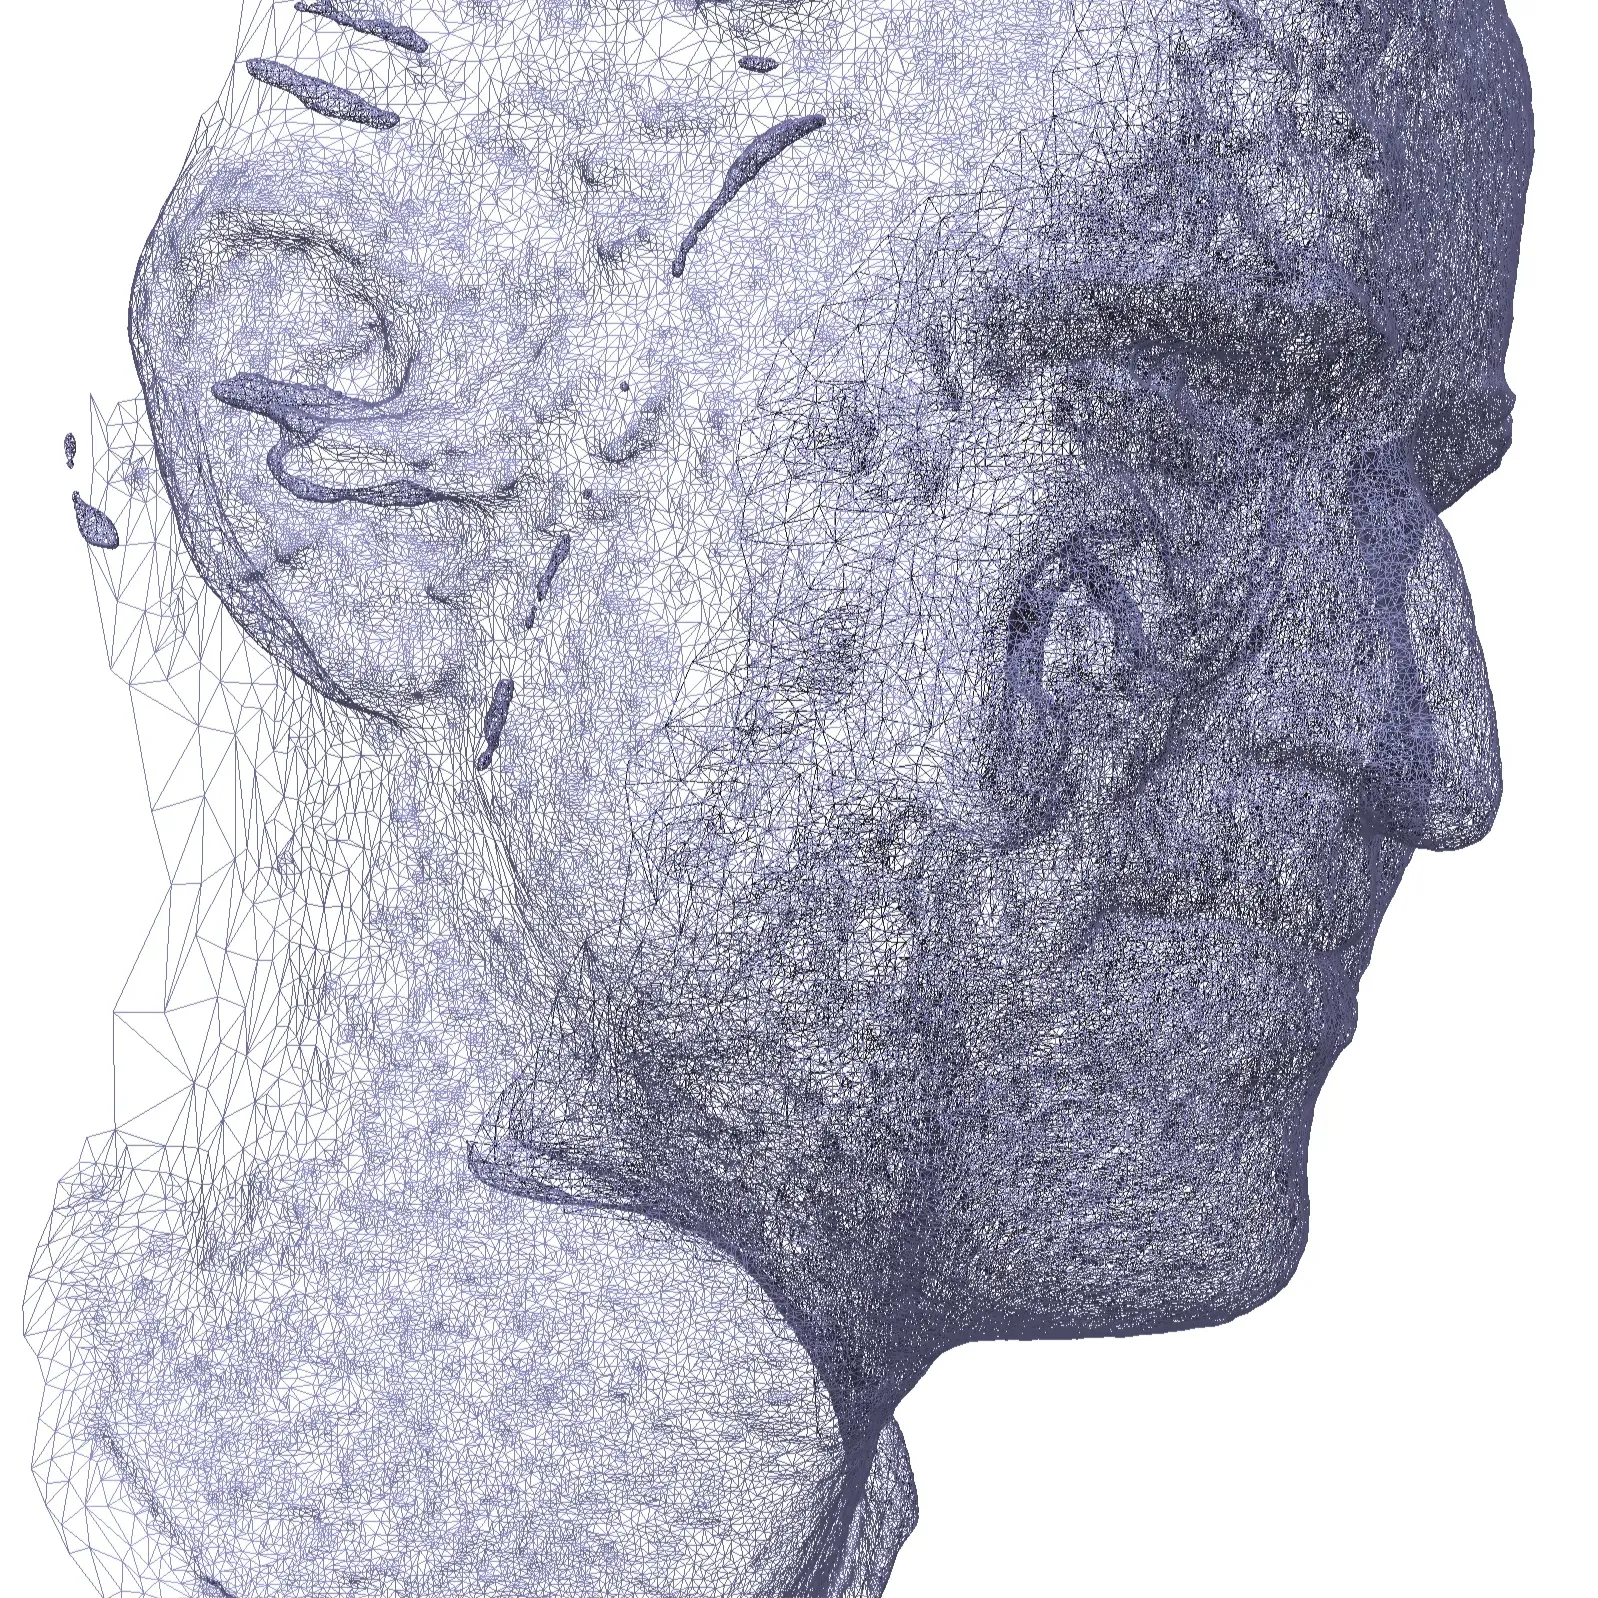
\includegraphics[width=\textwidth]{Figures/basics/rep1.png}
        \caption{Wireframe Mesh}
    \end{subfigure}
    \begin{subfigure}{0.48\linewidth}
        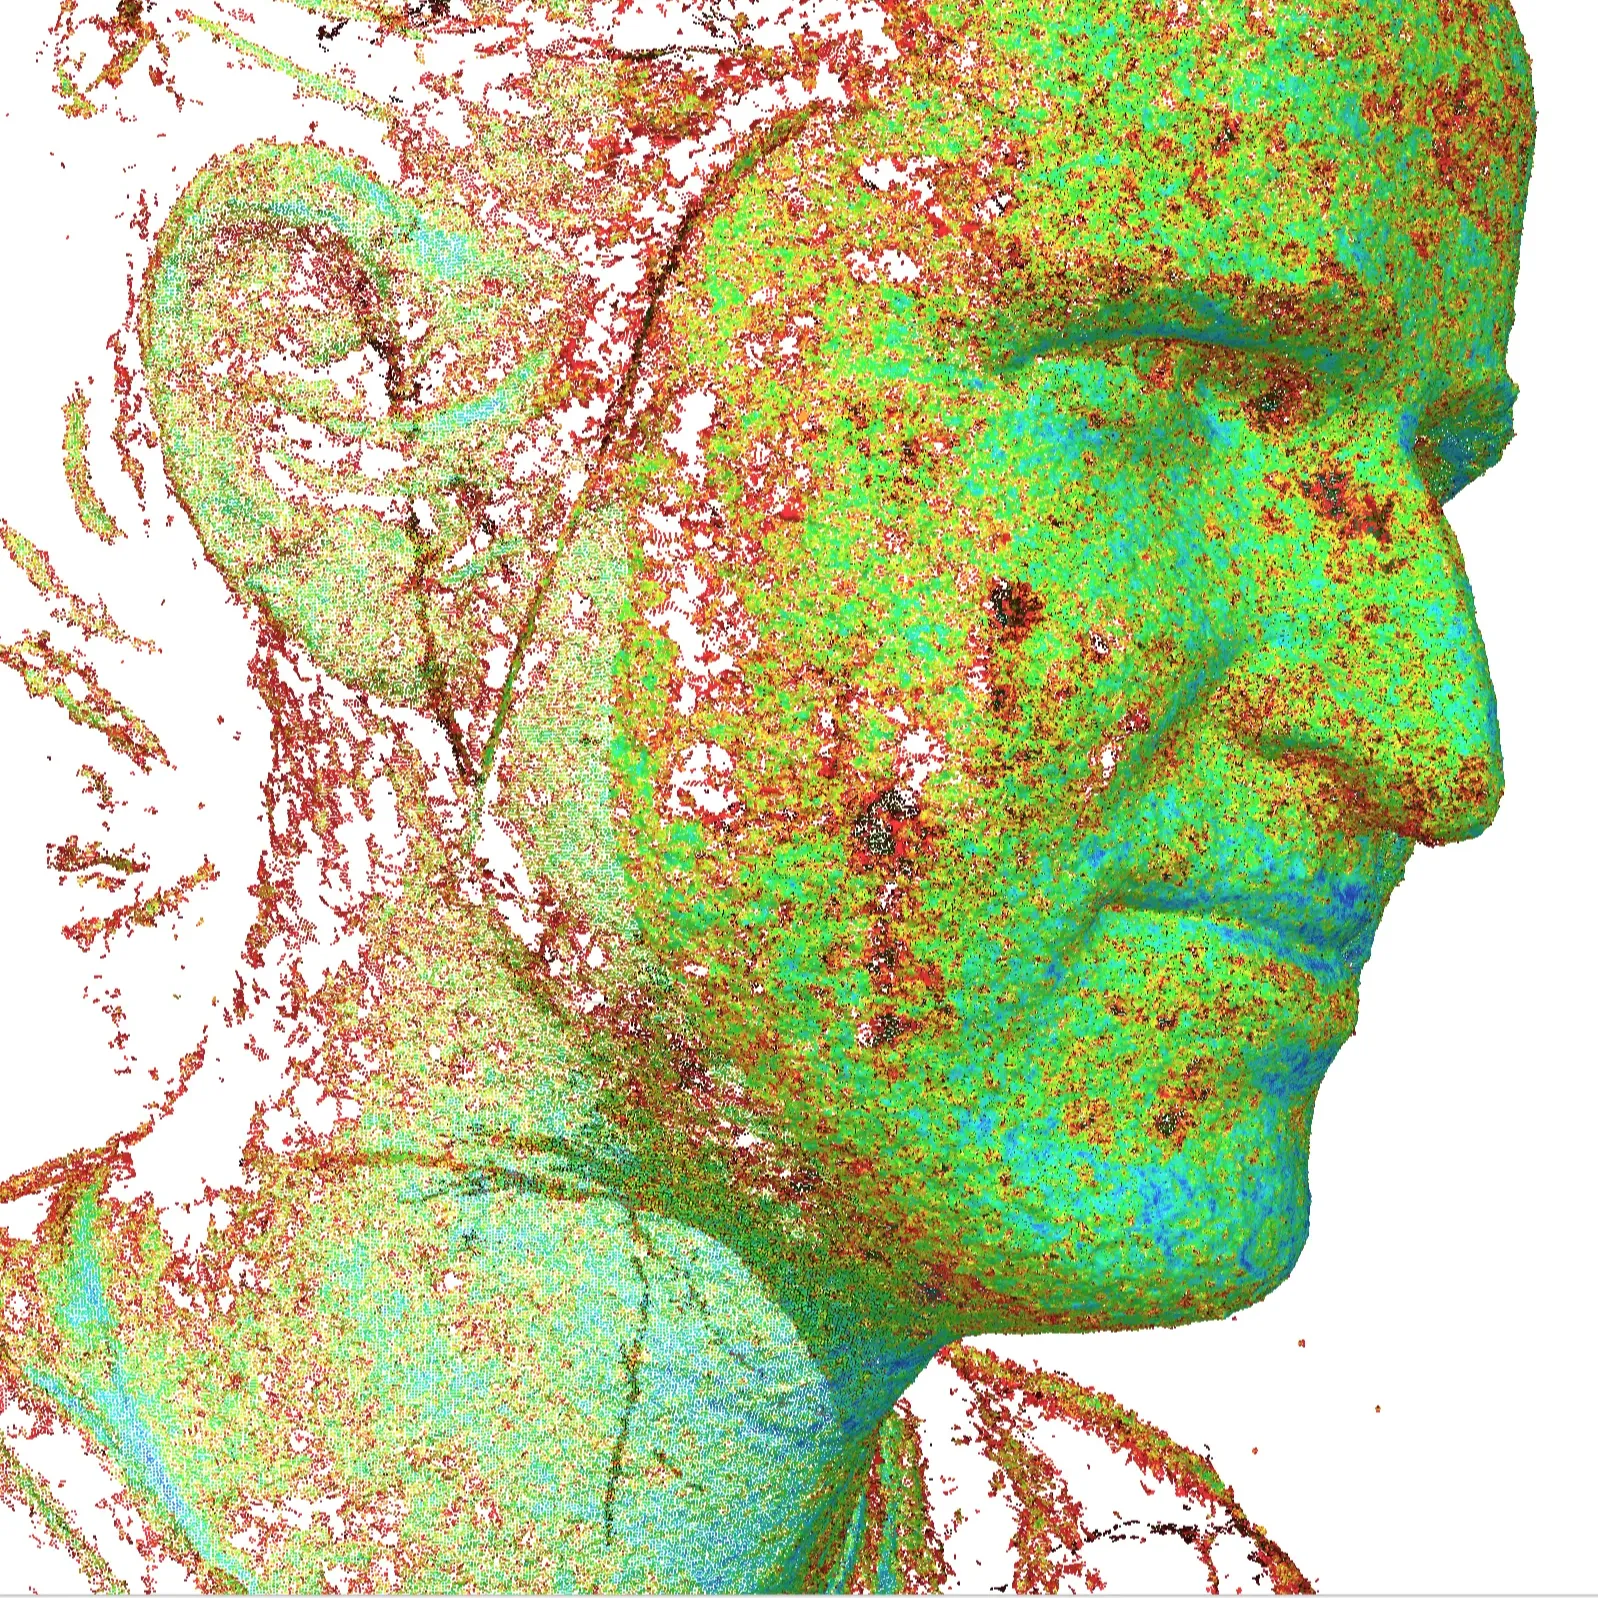
\includegraphics[width=\textwidth]{Figures/basics/rep3.png}
        \caption{Point Cloud (with accuracy level)}
    \end{subfigure}
    \begin{subfigure}{0.48\linewidth}
        \includegraphics[width=\textwidth]{Figures/basics/rep5.png}
        \caption{3D Gaussian Splatting}
    \end{subfigure}
    \caption{Overview of different 3D representations.}
    \label{fig:3D_representation}
\end{figure}

\subsection{Meshes}

Polygonal meshes, often referred to simply as meshes, are among the most commonly used 3D models in computer applications. These meshes provide a structured representation of surfaces through a network of polygonal faces, typically triangles, interconnected by shared vertices and edges \citep{Shirley.2002}. The fundamental components of a triangle mesh are a set of triangles formed by vertex triplets, along with the 3D positions of these vertices.

Meshes can store additional data at vertices, edges, or faces to facilitate texture mapping, shading, animation, and other operations. Vertex data commonly includes material parameters, texture coordinates, and irradiance values. These parameters are interpolated across triangles to create a continuous function over the mesh's surface. The mesh resolution, determined by the number of polygons or triangles, dictates the mesh's detail level and surface smoothness. Meshes are widely used in computer graphics due to their simplicity, flexibility, and support in most 3D rendering applications.

Despite their utility, meshes are less suitable for deformation and style transfer tasks due to their complex topology and diverse data structures \citep{Kang.2023}. Current mesh style transfer approaches leverage differentiable rendering \citep{Kato.2018} to deform and optimize meshes based on input text prompts \citep{Michel.2021} or image styles \citep{Gao.2022}. However, these methods often struggle with satisfactory deformations due to complex topologies, insufficient mesh resolution, and gradient computation challenges in differentiable rendering \citep{Kato.2020}.


\subsection{Point Clouds}

Point clouds represent 3D objects as a set of discrete points in space, each defined by its position and potentially additional information such as color or surface normals. The density of these points influences the resolution, allowing different parts of the model to have varying levels of detail. Point clouds are commonly generated from 3D scanning of real-world objects or environments using specialized devices or photogrammetry software. Unlike meshes, point clouds lack connectivity between points, making them flexible and precise but less suitable for tasks like rendering and animation \citep{Bassier.2020}.
Direct style transfer on point clouds is less common \citep{Cao.2020}, with point clouds often serving as intermediate representations in 3D reconstruction processes, such as mesh reconstruction or implicit function representation \citep{Mildenhall.2020, Kerbl.2023, Mu.2021}.

\subsection{Neural Radiance Fields}
Neural Radiance Fields (NeRF) \citep{Mildenhall.2020} model 3D scenes as a 5D function mapping 3D coordinates and view directions to color and opacity values. Using a multilayer perceptron (MLP), NeRF reconstructs scenes from a set of 2D images captured from various viewpoints. The MLP is trained to predict color and opacity along camera rays, minimizing the error between rendered and actual pixel colors.

Once trained, NeRF can generate photorealistic views of scenes from novel angles. However, NeRF's computational demands make it unsuitable for real-time applications. NeRF lacks a geometric scene representation, limiting its use in interactive tasks like collision detection or animation. Conversion to mesh or point cloud representations, such as through Signed Distance Fields (SDF) \citep{Darmon.2021} or the Marching Cubes algorithm \citep{Lorensen.1987}, can address these limitations.


\subsection{3D Gaussian Splatting}

With 3D Gaussian Splatting \Citep{Kerbl.2023}, a scene is represented as a collection of many 3D Gaussians. These 3D Gaussian objects can be thought of as fuzzy blobs that collectively approximate the geometry and appearance of the scene. With sufficient density and overlap, a collection of 3D Gaussians can effectively visualize a surface reconstruction of a real-world object or scene with high accuracy. A 3D Gaussian is chosen because, unlike triangles in meshes or points, it is differentiable and enables backward and forward pass in a neural network. Consequently, a 3D Gaussian can be easily modified to fit the real-world scene during optimization using gradient descent. Each Gaussian $g$ is defined by the following parameters:

\begin{itemize}[noitemsep]
    \item Mean $\mu$: The position (center) of the Gaussian in 3D space.
    \item Covariance Matrix $\Sigma$: The orientation and anisotropy (shape) of the Gaussian.
    \item Alpha $ \alpha$: The opacity of the Gaussian.
    \item Spherical Harmonics $c$: The color of the Gaussian.
\end{itemize}

A scene of 3D Gaussian Splatting can be denoted as a collection of 3D Gaussians $G = \{g_0, g_1, \dots ,g_N\}$, where each individual Gaussian $g = \{\mu , \Sigma , c, \alpha \}$.

As seen in Figure \ref{fig:3D_Gaussian_Splatting}, the learning process starts with initialization using a set of image tie points via Structure from Motion (SfM). Initial 3D Gaussians are placed at these tie points. \textcolor{green}{Green} arrows indicate the forward process where the actual scene is rendered from a camera view. \textcolor{orange}{Orange} arrows indicate the gradient flow where the ground truth/training image is compared to the rendered image and reprojected to the 3D scene to update the 3D Gaussians based on the loss. Specifically, the 3D Gaussian Splatting scene is trained with a modified L1 loss containing a D-SSIM \citep{Baker.2023} term. This process is repeated for each camera view in the training data until the loss converges. 3D Gaussian Splatting is more efficient than NeRF because it does not require expensive ray sampling for rendering and instead uses a differentiable rasterizer.

\begin{figure}
    \centering
    \includegraphics[width=\textwidth]{Figures/prelim_related/3D_gaussian_workflow.png}
    \caption{Overview of a 3DGS optimization process.}
    \label{fig:3D_Gaussian_Splatting}
\end{figure}

In addition, after every 100 iterations of the main optimization, a refinement process takes place. During this phase, the positioning and number of Gaussians in the scene are adaptively controlled to densely fit the scene's geometry and appearance, either by cloning, splitting, or moving them (indicated by the dotted arrow in Figure \ref{fig:3D_Gaussian_Splatting}). Furthermore, a pruning operation is carried out to cull or remove Gaussians with high transparency. As the optimization progresses, the Gaussians are refined, and the rendered image becomes more accurate based on the loss calculated from the difference between the rendered and ground truth images. The final result is a set of 3D Gaussians that represent the geometry and appearance of the scene.

\section{Image Style Transfer}

Image style transfer is a technique that allows one to transfer the style of one image to a content image. This technique is often used in computer vision to create stylized images and videos. The main idea behind image style transfer is to separate the content of an image from its style. The content of an image refers to the objects and their arrangement in the image, while the style of an image refers to the colors, textures, and patterns. By separating the content from the style, one can transfer the style of one image to a target image while preserving the content of the target image. This technique has been widely adopted in computer graphics to create stylized images and videos.

\subsection{Neural Style Transfer}

Pioneered by \textcite{Gatys.2015}, convolutional neural network (CNN)-based style transfer is a foundational technique for producing convincing artistic transformations beyond mere strokes and coloration changes. This approach, often called Neural Style Transfer (NST), employs a pre-trained CNN model, such as the Visual Geometry Group's VGG-19 network trained on the ImageNet dataset, to separate and recombine the content and style features of images. 

The content loss function $ \mathcal{L}_{content}$ is defined by the squared Euclidean distance between the feature representations of the content image $I_c$ and the generated image $I_g$ encoded by the VGG network at layer $l$ as follows:

\begin{equation}
    \mathcal{L}_{content} (I_c, I_g, l) = \frac{1}{2} \sum^{L}_{i,j} (VGG^{l}_{ci,j} -VGG^{l}_{gi,j} )^2
\end{equation}
where $VGG^l{ci,j}$ is the activation of the $i$-th convolution at the $j$-th position of layer $l$. The style loss exploits Gram-based visual texture modeling, defined by the squared Euclidean distance between the Gram-based style representations $\mathcal{G}$ from the VGG network for the style image $I_s$ and the generated image $I_g$:
\begin{equation}
    \mathcal{L}_{style} = \sum^{L}_{i,j} w_l \frac{1}{4N^2_l M^2_l} (\mathcal{G}^{l}_{ij} - \mathcal{G}^{l}_{ij})^2
\end{equation}
Combining with the content loss and the style loss across the layers, the  total loss is computed as follows:
\begin{equation}
    \mathcal{L}_{total}(I_s,I_c,I_g) = \alpha \mathcal{L}_{content}(I_c,I_g) + \beta \mathcal{L}_{style}(I_s,I_g)
\end{equation}
Here, $\alpha$ and $\beta$ are hyperparameters controlling the relative importance of content and style losses. The total loss $\mathcal{L}_{total}$ is minimized using gradient descent to generate the stylized image $I_g$.

Despite its foundational role, classical NST has limitations, including high computational cost and single-style optimization, requiring full re-optimization for each new style \Citep{Chen.2023}. More advanced methods have emerged to support multiple styles within a single network \Citep{Varlamova.2022}. However, NST often struggles to deeply understand the interplay between content and style, relying on separate optimization processes that may not capture this relationship comprehensively \Citep{Jing.2020}.

\subsection{Diffusion Models}

With the rising public interest in deep learning-based techniques, diffusion-based methods have garnered significant attention. One of the prominent approaches is the Latent Diffusion Model (LDM), first proposed by \textcite{Rombach.2022}. Stable Diffusion (SD) is implemented as a Latent Text-to-Image Diffusion pipeline, trained on text-image pair datasets to generate images from textual prompts or descriptions. Formally, an SD model samples a 3-channeled image $I \in \mathbb{R}^{3 \times H \times W}$ from a conditional distribution $p(I | y)$, where $y$ is the textual input prompt.

\begin{figure}[ht]
    \centering
    \includegraphics[width=0.8\textwidth]{Figures/prelim_related/sd-workflow.png}
    \caption{Simplified overview of the Stable Diffusion pipeline.}
    \label{fig:stable_diffusion}
\end{figure}

SD consists of three main components: a Variational Autoencoder (VAE), a U-Net architecture, and a conditioning encoder. The VAE encodes the image into a latent representation $z$ and decodes it back to an image. It is trained separately to compress the image into a much smaller latent space that captures its semantic features. The U-Net is a convolutional neural network responsible for image generation through the denoising of the latent space with the help of embeddings. The U-Net architecture is illustrated in Figure \ref{fig:controlnet}a. In the text-to-image generation SD pipeline, the conditioners are textual embeddings obtained by encoding textual descriptions using a Transformer language model, often CLIP \citep{Radford.2021}.

Training an SD model involves forward and backward propagation (illustrated by \textcolor{green}{green} and \textcolor{orange}{orange} arrows in Figure \ref{fig:stable_diffusion}). During forward propagation, a sample image $I$ is compressed into a latent representation $z$ to capture its semantic features using the VAE encoder $\mathcal{E}$, such that $z_0 = \mathcal{E}(I)$. Gaussian noise $x$ is then added at each step $t \in T$ according to a noise schedule $0 < \beta_1 < \dots < \beta_T < 1$ to produce a noisy latent $z_t = z + \beta_t$. At the last step $T$, the latent consists purely of Gaussian noise.

Backward propagation, where denoising occurs, iteratively reverts the latent $z_T$ to $z_0$ following the same schedule. The U-Net, conditioned on the textual embedding via a cross-attention mechanism (\textcolor{yellow}{yellow} arrow), predicts the total noise $\hat{\beta}_t$ in $z_t$ to estimate $z_0$. Since the predicted noise $\hat{\beta}_t$ is likely inaccurate, only a fraction $x$ of this noise is removed from $z_t$, such that $z_{t-1} = z_t - x \hat{\beta}_t$. This process repeats for every step $t$ until the loss converges. The aim is to optimize the noise distribution at each step by minimizing the loss between the predicted noise and the actual noise. This loss is computed as the negative log likelihood of the predicted noise given the actual noise. The process continues for all images in the dataset until convergence, with sampled images $I' \approx I$.

Using an SD model for text-to-image generation involves only the backward process, starting with pure Gaussian noise and gradually refining it using the user's text prompt as denoising guidance. The fully denoised latent is decoded via the VAE decoder to produce the final image.

Editing facial images with SD typically requires the face to occupy a large portion of the image. As shown in Figure \ref{fig:unpreprocessed}, stylizing Photodome images without sufficient preprocessing often leads to undesirable facial deformations or non-visible changes. This is because the model is trained on a dataset of images where faces are centered and occupy significant space. Consequently, the model struggles to generalize to images where faces are off-center or occupy a smaller area. This limitation can be mitigated by preprocessing images to center the face and crop them to the desired size before stylization. This challenge also applies to other SD pipelines like InstructPix2Pix \citep{Brooks.2023}, which will be discussed in the next section.

\begin{figure}
	\centering
	\begin{subfigure}{0.48\linewidth}
		\includegraphics[width=\textwidth]{Figures/unpreprocessed/0-1-5-1-294_210300_834.JPG}
        \includegraphics[width=\textwidth]{Figures/unpreprocessed/0-2-6-2-303_210300_871.JPG}
		\caption{Raw Photodome captures}
	\end{subfigure}
	\begin{subfigure}{0.48\linewidth}
		\includegraphics[width=\textwidth]{Figures/failed/sd_unprocessed/0-1-5-1-294_210300_834.JPG}
        \includegraphics[width=\textwidth]{Figures/failed/sd_unprocessed/0-2-6-2-303_210300_871.JPG}
		\caption{"Photo of angry man"}
	\end{subfigure}
	\caption{Stylization of Photodome images without sufficient preprocessing steps tends to results in either undesirable facial deformation (top) or non-visible changes (bottom).}
	\label{fig:unpreprocessed}
\end{figure}

\subsubsection{InstructPix2Pix}
Today SD branches out from its original purpose to incorporate other technology in order to produce more convincing results or to accomplish different tasks. InstructPix2Pix \Citep{Brooks.2023} modifies the original SD model to enable image stylization using human instructions as opposed to the common text prompt used in the original SD model. This is done by training other SD model and usage of a Large Language Model (LLM) to generate several intermediate synthetic training datasets as seen in Figure \ref{fig:instructpix2pix}. To generate the initial dataset, \Textcite{Brooks.2023} first manually create 700 \textit{<source caption, target caption, edit instruction>} triplets, then leverage them to fine-tune a \textit{GPT-3} language model to make it generate a larger amount multi-modal synthetic dataset consisting of 454 thousand triplets. To transform the \textit{<source caption, target caption>} pairs into \textit{<source image, target image>} pairs, they use \textit{Prompt2Prompt}, a modified SD model \Citep{Hertz.2022} that enables intuitive text-based editing of real images with the SD model.
Finally, the \textit{<source image, target image, edit instruction>} triplets are used to fine-tune a SD model into the InstructPix2Pix model.
\begin{figure}[h]
    \centering
    \includegraphics[width=0.8\textwidth]{Figures/prelim_related/instructpix2pix_training.png}
    \caption{Overview of InstructPix2Pix model training workflow.}
    \label{fig:instructpix2pix}
\end{figure}

Unlike other SD pipelines, InstructPix2Pix and Prompt2Prompt are considered style transfer techniques as they can plausibly transform an image by altering its content and style while preserving similarity to the original image, rather than being fully generative models. Figures \ref{fig:instructpix2pix_initial_4-5-1} and \ref{fig:instructpix2pix_initial_2-4-2} show experimental results of the InstructPix2Pix model from different view angles during the initial research, using two different configurations: default and modified guidance scales. By setting the lower textual guidance scale to 5 and the image guidance scale to 2, the model produces plausible results.

\begin{figure}[ht]
    \centering
    \begin{subfigure}{0.18\linewidth}
        \includegraphics[width=\textwidth]{Figures/resized_images/0-4-5-1-5648_230239_266.JPG}
		\caption{Original}
	\end{subfigure}
    \begin{subfigure}{0.18\linewidth}
        \includegraphics[width=\textwidth]{Figures/naive/default/ipix2pix_sven_stone/0-4-5-1-5648_230239_266.png}
        \includegraphics[width=\textwidth]{Figures/naive/low_cfg/ipix2pix_sven_stone/0-4-5-1-5648_230239_266.png}
    \caption{Stone statue}
	\end{subfigure}
    \begin{subfigure}{0.18\linewidth}
        \includegraphics[width=\textwidth]{Figures/naive/default/ipix2pix_sven_fauvism/0-4-5-1-5648_230239_266.png}
        \includegraphics[width=\textwidth]{Figures/naive/low_cfg/ipix2pix_sven_fauvism/0-4-5-1-5648_230239_266.png}
        \caption{Fauvism}
	\end{subfigure}
    \begin{subfigure}{0.18\linewidth}
        \includegraphics[width=\textwidth]{Figures/naive/default/ipix2pix_sven_elf/0-4-5-1-5648_230239_266.png}
        \includegraphics[width=\textwidth]{Figures/naive/low_cfg/ipix2pix_sven_elf/0-4-5-1-5648_230239_266.png}
        \caption{Tolkien elf}
	\end{subfigure}
    \begin{subfigure}{0.18\linewidth}
        \includegraphics[width=\textwidth]{Figures/naive/default/ipix2pix_sven_clown/0-4-5-1-5648_230239_266.png}
        \includegraphics[width=\textwidth]{Figures/naive/low_cfg/ipix2pix_sven_clown/0-4-5-1-5648_230239_266.png}
		\caption{Clown}
	\end{subfigure}
    \caption{From camera 4-5-1, initial experimental test of the InstructPix2Pix model with various prompts. Top: results with default settings. Bottom: results with a low textual guidance scale.}
    \label{fig:instructpix2pix_initial_4-5-1}

\end{figure}

\begin{figure}
    \begin{subfigure}{0.18\linewidth}
        \includegraphics[width=\textwidth]{Figures/resized_images/0-2-4-2-293_210300_829.JPG}
		\caption{Original}
	\end{subfigure}
    \begin{subfigure}{0.18\linewidth}
        \includegraphics[width=\textwidth]{Figures/naive/default/ipix2pix_sven_stone/0-2-4-2-293_210300_829.png}
        \includegraphics[width=\textwidth]{Figures/naive/low_cfg/ipix2pix_sven_stone/0-2-4-2-293_210300_829.png}
        \caption{Stone statue}
	\end{subfigure}
    \begin{subfigure}{0.18\linewidth}
        \includegraphics[width=\textwidth]{Figures/naive/default/ipix2pix_sven_fauvism/0-2-4-2-293_210300_829.png}
        \includegraphics[width=\textwidth]{Figures/naive/low_cfg/ipix2pix_sven_fauvism/0-2-4-2-293_210300_829.png}
        \caption{Fauvism}
	\end{subfigure}
    \begin{subfigure}{0.18\linewidth}
        \includegraphics[width=\textwidth]{Figures/naive/default/ipix2pix_sven_elf/0-2-4-2-293_210300_829.png}
        \includegraphics[width=\textwidth]{Figures/naive/low_cfg/ipix2pix_sven_elf/0-2-4-2-293_210300_829.png}
        \caption{Tolkien elf}
	\end{subfigure}
    \begin{subfigure}{0.18\linewidth}
        \includegraphics[width=\textwidth]{Figures/naive/default/ipix2pix_sven_clown/0-2-4-2-293_210300_829.png}
        \includegraphics[width=\textwidth]{Figures/naive/low_cfg/ipix2pix_sven_clown/0-2-4-2-293_210300_829.png}
		\caption{Clown}
    \end{subfigure}
    \caption{From camera 2-4-2, initial experimental test of the InstructPix2Pix model with various prompts. Top: results with default settings. Bottom: results with a low textual guidance scale.}
    \label{fig:instructpix2pix_initial_2-4-2}

\end{figure}


\subsubsection{ControlNet}
Rather than retraining an SD model, \textcite{Zhang.2023} demonstrates that one can add a control network to a base SD pipeline to enable different conditioning inputs through ControlNet. ControlNet preserves the properties and capabilities of the base model by locking its parameters and adding a trainable copy of the default UNet encoding layers to the pipeline, as shown in Figure \ref{fig:controlnet}. As a result, conditional inputs such as depth maps, masks, edges, or poses can be applied to the original pipelines. Similar to text or conditioning images, these inputs are converted into latent representations and used as additional conditioners during the ControlNet-modified diffusion process. Consequently, the SD pipeline can perform more complex and diverse style transfer tasks. 

During the initial research for this thesis, ControlNet was found to be more generative in nature than editing, resulting in stylizations that barely resembled the original human face and often included facial deformations, particularly when combined with InstructPix2Pix. As shown in Figure \ref{fig:controlnet_failed}, stylization with ControlNet led to extreme alterations of the original even with several conditioners and a low textual guidance scale.

\begin{figure}[ht]
    \centering
    \includegraphics[width=0.7\textwidth]{Figures/prelim_related/controlnet.png}
    \caption{Comparison between the default UNet architecture of an SD pipeline (a) and ControlNet \citep{Zhang.2023} (b). In ControlNet, the attention mechanism is applied to the copy block instead of the main UNet block.}
    \label{fig:controlnet}
\end{figure}

Additionally, the random seed in ControlNet appears to have a larger impact on the results, particularly regarding their resemblance to the original inputs, compared to the original InstructPix2Pix pipeline. However, due to the popularity of this approach and SD in general, many contributors have published their versions of ControlNet with different architectures and training data. As such, this limitation may have been addressed in the latest versions of the pipelines and models.

\begin{figure}[ht]
    \centering
    \begin{subfigure}{0.18\linewidth}
        \includegraphics[width=\textwidth]{Figures/resized_images/0-4-5-1-5648_230239_266.JPG}
        \includegraphics[width=\textwidth]{Figures/resized_images/0-2-4-2-293_210300_829.JPG}
        \includegraphics[width=\textwidth]{Figures/resized_images/0-C-5-1-5386_212530_574.JPG}
		\caption{Originals}
	\end{subfigure}
    \begin{subfigure}{0.18\linewidth}
        \includegraphics[width=\textwidth]{Figures/failed/controlnet/canny/0-4-5-1-5648_230239_266_canny.png}
        \includegraphics[width=\textwidth]{Figures/failed/controlnet/canny/0-2-4-2-293_210300_829_canny.png}
        \includegraphics[width=\textwidth]{Figures/failed/controlnet/canny/0-C-5-1-5386_212530_574_canny.png}
		\caption{Canny edges}
	\end{subfigure}
    \begin{subfigure}{0.18\linewidth}
        \includegraphics[width=\textwidth]{Figures/failed/controlnet/openpose/0-4-5-1-5648_230239_266_openpose.png}
        \includegraphics[width=\textwidth]{Figures/failed/controlnet/openpose/0-2-4-2-293_210300_829_openpose.png}
        \includegraphics[width=\textwidth]{Figures/failed/controlnet/openpose/0-C-5-1-5386_212530_574_openpose.png}
        \caption{Face poses}
	\end{subfigure}
    \begin{subfigure}{0.18\linewidth}
        \includegraphics[width=\textwidth]{Figures/failed/controlnet/depth/0-4-5-1-5648_230239_266_depth.png}
        \includegraphics[width=\textwidth]{Figures/failed/controlnet/depth/0-2-4-2-293_210300_829_depth.png}
        \includegraphics[width=\textwidth]{Figures/failed/controlnet/depth/0-C-5-1-5386_212530_574_depth.png}
        \caption{Depth maps}
	\end{subfigure}
    \begin{subfigure}{0.18\linewidth}
        \includegraphics[width=\textwidth]{Figures/failed/controlnet/0-4-5-1-5648_230239_266.png}
        \includegraphics[width=\textwidth]{Figures/failed/controlnet/0-2-4-2-293_210300_829.png}
        \includegraphics[width=\textwidth]{Figures/failed/controlnet/0-C-5-1-5386_212530_574.png}
		\caption{Results}
	\end{subfigure}
    \caption{Failed stylization results of ControlNet using the InstructPix2Pix pipeline with Canny edges, OpenPose for facial landmarks, and depth maps as conditioners, with the prompt "Turn him into a stone statue" and seed 33. Notice that the results not only barely resemble the original human face but also do not conform to the textual prompt.}
    \label{fig:controlnet_failed}
\end{figure}

\subsubsection{LoRa}

\textcite{Hu.2021} propose a novel fine-tuning method for pre-trained diffusion models called LoRa (Low-Rank Adaptation of Large Language Models). Traditionally, fine-tuning large language models such as GPT-3 is computationally expensive, as it requires updating all of the model's parameters. LoRa addresses this issue by introducing trainable low-rank decomposition matrices, which correspond to some of the base model's parameters. This allows for partial reparameterization of the model, significantly reducing the computational cost of fine-tuning. In the context of diffusion-based pipelines, LoRa has been used to modify the text encoders and/or denoising networks to emphasize (or de-emphasize) certain concepts or introduce new ones in the existing model. Building upon LoRa, \textcite{Yeh.2023} propose a new framework called LyCORIS (LoRa beYond Conventional methods, Other Rank adaptation Implementations) for diffusion-based models. This framework collects and analyzes various metrics and LoRa-based fine-tuning methods specifically for text-to-image generative models.

\section{Losses and metrics}

\subsection{$\mathcal{L}_1$ Loss}
The $\mathcal{L}_1$ loss, also known as mean absolute error (MAE), is a common loss function used in image processing tasks like image denoising, super-resolution, or image reconstruction. In the 2D domain, $\mathcal{L}_1$ loss is computed as the average of the absolute differences between each pixel in the predicted image and the corresponding pixel in the ground truth (original) image. It measures the difference between the predicted pixel values of an image and the true pixel values in a straightforward, absolute manner. The $\mathcal{L}_1$ loss is formulated as:
\begin{equation}
    \label{}
    \mathcal{L}_1(I_{pred},I_{true} ) = \frac{1}{N}  \sum ^N_{i = 1} | I_{pred}(i) - I_{true}(i)|
\end{equation}
where $N$ is the total number of pixels in the image, $I_{pred}(i)$ and $I_{true}(i)$ are the predicted and ground truth pixel values at location $i$, respectively. In the context of 3D stylization, $\mathcal{L}_1$ quantifies the difference between the expected stylization result and the actual stylized rendering of the 3D object.

\subsection{PSNR}
Peak Signal-to-Noise Ratio (PSNR) is a logarithmic measure that compares the maximum possible pixel value of an image (signal) to the difference (noise) between the original image and the distorted or reconstructed image. Mathematically, PSNR is defined as:

\begin{equation}
    PSNR(I_{pred},I_{true} ) = 10 \cdot \log_{10} (\frac{MAX_I^2}{\mathcal{L}_1(I_{pred},I_{true} )})
\end{equation}
where $MAX_I$ is the maximum possible pixel value of the image.

PSNR is widely used to assess the quality of lossy image compression methods like JPEG, and in other tasks such as image denoising, restoration, and super-resolution. In the 3D domain, PSNR serves as a quantitative metric to evaluate the quality of the reconstructed 2D views compared to the ground truth 2D views captured from a real-world object or scene. It can also evaluate the stylization quality of a 3D object from a camera view given the corresponding stylized image.

PSNR values are measured in decibels (dB). A typical good-quality image will have a PSNR value between 30–50 dB, where values above 40 dB are considered excellent.

\subsection{SSIM and DSSIM}

The DSSIM loss is derived from the SSIM (Structural Similarity Index), which compares two images based on structural information like luminance, contrast, and structure \citep{Wang.2004, Nilsson.2020}. SSIM aims to capture the human visual system's perception of similarity rather than simply relying on pixel-level differences. DSSIM measures the dissimilarity between images. In the context of image stylization, SSIM and DSSIM quantify the perceived similarity of the stylized image compared to the expected result.

\subsubsection{SSIM}
The SSIM formula comprises luminance, contrast, and structural components:
\begin{equation}
    \mathsf{SSIM}(I_{pred}, I_{true}) = l(I_{pred}, I_{true})^\alpha \cdot c(I_{pred}, I_{true})^\beta \cdot s(I_{pred}, I_{true})^\gamma
\end{equation}
where $l(I_{pred}, I_{true})$ is the luminance difference, $c(I_{pred}, I_{true})$ is the contrast difference, and $s(I_{pred}, I_{true})$ is the structural difference between the predicted image $I_{pred}$ and the ground truth $I_{true}$. The parameters $\alpha$, $\beta$, and $\gamma$ are weights for the contribution of each component.

The luminance, contrast, and structure components are defined as:
\begin{equation}
    l(I_{pred}, I_{true}) = \frac{2\mu_{pred}\mu_{true} + c_1}{\mu_{pred}^2 + \mu_{true}^2 + c_1}
\end{equation}

\begin{equation}
    c(I_{pred}, I_{true}) = \frac{2\sigma_{pred}\sigma_{true} + c_2}{\sigma_{pred}^2 + \sigma_{true}^2 + c_2}
\end{equation}

\begin{equation}
    s(I_{pred}, I_{true}) = \frac{\sigma_{pred, true} + c_3}{\sigma_{pred} \sigma_{true} + c_3}
\end{equation}

Here, $\mu_{pred}$ and $\mu_{true}$ are the pixel sample means of the predicted and ground truth images, respectively, denoting luminance. $\sigma_{pred}$ and $\sigma_{true}$ are the standard deviations, representing contrast. $\sigma_{pred, true}$ is the covariance between the images, denoting structure. Constants $c_1$, $c_2$, and $c_3$ are variables to stabilize the division when the denominator is weak.

\subsubsection{DSSIM}
To convert SSIM into a dissimilarity measure for use as a loss function, DSSIM is defined as:

\begin{equation}
    \mathsf{DSSIM}(I_{pred}, I_{true}) = \frac{1-SSIM(I_{pred}, I_{true})}{2}
\end{equation}

DSSIM is commonly used in tasks like image super-resolution, denoising, and style transfer, where structural integrity is crucial. In 3D stylization, DSSIM is particularly relevant when using 2D multi-view priors, as inconsistencies in stylization can compromise the quality of the resulting 3D object.

\subsection{CLIP Similarity Metrics}
CLIP (Contrastive Language-Image Pre-training) \citep{Radford.2021} is a convolutional neural network model developed by OpenAI that relates text and images in a shared embedding space. Several types of similarities can be computed using CLIP to measure relationships between text and images or between images themselves. Some uses of CLIP include Text-to-Image Direction Similarity (CTIDS) and Image-Image Similarity (CIIS).

\subsubsection{Text-to-Image Direction Similarity}
CLIP Text-Image Direction Similarity (CTIDS) measures how closely the semantic direction implied by a text prompt matches the direction between two images in CLIP's embedding space. It compares the vector direction from one image to another with the vector direction from a text prompt to one of the images. This measure is useful for evaluating how well a textual description captures the semantic change between two images.

\subsubsection{Image-Image Similarity}
CLIP Image-Image Similarity (CIIS) measures the similarity between two images purely based on their visual content as encoded in CLIP's image embedding space. CLIP embeds images into a vector space where visually and semantically similar images are positioned closer together. Image-Image Similarity is typically computed using cosine similarity between these image embeddings. The closer the cosine similarity is to 1, the more similar the images are. This is particularly useful for comparing multi-view images in the dataset and assessing the consistency of their stylization.

\subsection{FID}
FID (Fréchet Inception Distance) is a metric used to assess the quality of generated images by comparing them to a set of real images. In the context of image stylization, FID measures how closely the stylized images match the distribution of the original content or real-world images. It is particularly useful for evaluating generative models, such as style transfer networks, to assess how realistic and stylistically coherent the generated (stylized) images are, as well as how well the content of the real image is preserved in the stylized image. Lower FID indicates that the distribution of stylized images is closer to the original image distribution or the target style's distribution, implying better stylization quality and higher content preservation.

FID is computed using the following formula:
\begin{equation}
    FID = ||\mu_{real} - \mu _{style} + \mathsf{Tr} (\Sigma _{real} + \Sigma _{style} - 2(\Sigma_{real} \Sigma_{style} )^\frac{1}{2})
\end{equation}
where $\mu_{real}$ and $\mu_{style}$ are the means of the real (original) and generated (stylized) images' feature representations, $\Sigma_{real}$ and $\Sigma_{style}$ are the covariance matrices of the real and generated images' feature representations, and $\mathsf{Tr}$ is the trace of a matrix (the sum of its elements on the main diagonal).

\subsection{LPIPS}
LPIPS (Learned Perceptual Image Patch Similarity) \citep{Zhang.2018} is a perceptual similarity metric that measures the similarity between two images based on their perceptual features. LPIPS is designed to capture the perceptual similarity between images as perceived by humans. It uses deep features from various pre-trained deep neural networks, such as VGG or AlexNet, to serve as the basis of the metric, providing a closer correspondence to human perception of similarity than classical metrics like SSIM.

LPIPS is particularly useful for evaluating image quality in cases where spatial ambiguities are a factor. It is computed by comparing the perceptual features of two images using a pre-trained deep neural network. Lower LPIPS values indicate higher perceptual similarity between the images. However, there is no clearly defined upper bound. During initial research, it was observed that two completely different images could have an LPIPS value around 0.6. Moreover, no known documentation clarifies how LPIPS values scale in terms of image quality or similarity.


\chapter{Related Work}
\label{chap:relatedwork}

\section{3D Style Transfer}

The initial objective was to explore the possibility of style transfer on 3D avatars, leading to the relatively new field of 3D style transfer in computer vision. 3D neural stylization or style transfer refers to applying neural stylization techniques to modify the visual appearance and aesthetic characteristics of pre-existing 3D digital representations \citep{Chen.2023}. To fuse 3D representation with a new style, two key factors must be considered: 3D content preservation and style transformation. In the context of 3D avatars, geometry represents the shape of the avatar, while texture represents its color. Thus, 3D avatar style transfer can be divided into two main categories: geometry-based style transfer and texture-based style transfer. Geometry-based style transfer modifies the shape of the 3D avatar, whereas texture-based style transfer alters the color of the 3D avatar. Successful style transfer on 3D avatars requires considering both the geometry and texture of the input avatar, as well as the style guidance, which can be provided as a text prompt \citep{Nguyen-Phuoc.2023, Zhang.2023, Mendiratta.2023} or a reference image \citep{Han.2021, Abdal.2023, Zhang.2024, Jaganathan.2024}. 

Some works extend image-to-image style transfer networks to directly stylize 3D objects \citep{Kang.2023}. Others leverage 2D priors to guide 3D stylization results in various representations, such as point clouds \citep{Cao.2020, Segu.2020, Luo.2021}, meshes \citep{Yin.2021, Nguyen-Phuoc.2023, Kang.2023, Yang.2023}, and implicit functions like neural radiance fields \citep{Haque.2023, Kamata.2023, Patashnik.2024}, and more recently, Gaussian Splatting \citep{Wang.2024, Liu.2024, Wu.2024, Chen.2024, Jaganathan.2024}. Many of these methods are too complex for the specific goal of stylizing a 3D avatar using multi-view images. However, several works have inspired this thesis, providing valuable insights into 3D style transfer on head avatars and a potential workflow for multi-view image style transfer.

\section{Exemplar-based 3D Portrait Stylization}
\textcite{Han.2021} propose a pipeline to generate a stylized 3D human face model with exaggerated geometry and texture transferred from a 2D cartoon image. The authors introduce a two-stage approach that disentangles the geometric and texture domains. In the first stage, the method generates a coarse 3D face stylized geometry from a real facial photo and a 2D caricature image as the style reference. This is achieved by using their multi-modal landmark translation network to map all 68 facial landmarks of the style image and the real photo, enabling the creation of a coarse global shape of the 3D face model for a deformation network using a differentiable rasterizer such as SoftRas \citep{Liu.2019}. 

In the second stage, the method focuses on performing artistic style transfer on the canonical texture using STROTSS \citep{Kolkin.2019}, while keeping the geometry fixed. A differentiable renderer is employed to render the textured model into different views and optimize the texture through a multi-view framework. The pipeline also incorporates a novel multi-view loss function to preserve the identity of the person in the real photo. As a result, it can perform both semantic and artistic style transfer through mesh deformation and texture editing. However, the pipeline is limited to a single style image and a single real photo. Upon accessing the implementation, it was observed that the pipeline functions effectively only in a very specific setting, as demonstrated in their example, and requires significant manual intervention. Figure \ref{fig:stross_texture_style} shows the application of the example style images to Photodome images. Despite the pipeline's capability to learn styles from a large dataset of style images and preprocess these images, only two compatible style images are provided.

\begin{figure}
    \centering
    \begin{subfigure}{0.22\linewidth}
        \includegraphics[width=\textwidth]{Figures/white.png}
        \includegraphics[width=\textwidth]{Figures/failed/stross/textures/00016_style.jpg}
        \includegraphics[width=\textwidth]{Figures/failed/stross/textures/00059_style.jpg}
	\end{subfigure}
    \begin{subfigure}{0.22\linewidth}
        \includegraphics[width=\textwidth]{Figures/failed/stross/textures/masked/masked_head_8-8-5-1_123851_791.png}
        \includegraphics[width=\textwidth]{Figures/failed/stross/textures/16/stylized_view_8-8-5-1_123851_791.png}
        \includegraphics[width=\textwidth]{Figures/failed/stross/textures/59/stylized_view_8-8-5-1_123851_791.png}
	\end{subfigure}
    \begin{subfigure}{0.22\linewidth}
        \includegraphics[width=\textwidth]{Figures/failed/stross/textures/masked/masked_head_8-5-3-2_123851_842.png}
        \includegraphics[width=\textwidth]{Figures/failed/stross/textures/16/stylized_view_8-5-3-2_123851_842.png}
        \includegraphics[width=\textwidth]{Figures/failed/stross/textures/59/stylized_view_8-5-3-2_123851_842.png}
	\end{subfigure}
    \begin{subfigure}{0.22\linewidth}
        \includegraphics[width=\textwidth]{Figures/failed/stross/textures/masked/masked_head_8-C-5-1_123851_737.png}
        \includegraphics[width=\textwidth]{Figures/failed/stross/textures/16/stylized_view_8-C-5-1_123851_737.png}
        \includegraphics[width=\textwidth]{Figures/failed/stross/textures/59/stylized_view_8-C-5-1_123851_737.png}
	\end{subfigure}
    \caption{Experimentation of STROTSS pipeline with various style images applied to the masked Photodome images. The effect of landmarks translation between the style image and the Photodome images is visible in the stylized images even though it can be inaccurate in certain regions resulting in inconsistencies across views.}
    \label{fig:stross_texture_style}

\end{figure}

Furthermore, the pipeline does not provide an end-to-end solution, making it difficult to reproduce the results or adapt it for this thesis. For experimentation purposes in initial research, their style transfer pipeline was used with the Photodome dataset but without their deformation and reconstruction pipeline. Instead, a canonical 3D avatar was built using photogrammetric reconstruction, and the stylized images were remapped to its UV coordinates. The results are shown in Figure \ref{fig:stross_texture_fit}.

\begin{figure}
    \centering
    \begin{subfigure}{0.18\linewidth}
        \includegraphics[width=\textwidth]{Figures/failed/stross/3d/snapshot09.png}
        \includegraphics[width=\textwidth]{Figures/failed/stross/3d/snapshot10.png}
        \includegraphics[width=\textwidth]{Figures/failed/stross/3d/snapshot11.png}
	\end{subfigure}
    \begin{subfigure}{0.18\linewidth}
        \includegraphics[width=\textwidth]{Figures/failed/stross/3d/snapshot14.png}
        \includegraphics[width=\textwidth]{Figures/failed/stross/3d/snapshot13.png}
        \includegraphics[width=\textwidth]{Figures/failed/stross/3d/snapshot12.png}
	\end{subfigure}
    \begin{subfigure}{0.18\linewidth}
        \includegraphics[width=\textwidth]{Figures/failed/stross/3d/snapshot15.png}
        \includegraphics[width=\textwidth]{Figures/failed/stross/3d/snapshot16.png}
        \includegraphics[width=\textwidth]{Figures/failed/stross/3d/snapshot17.png}
	\end{subfigure}
    \begin{subfigure}{0.18\linewidth}
        \includegraphics[width=\textwidth]{Figures/failed/stross/3d/snapshot20.png}
        \includegraphics[width=\textwidth]{Figures/failed/stross/3d/snapshot19.png}
        \includegraphics[width=\textwidth]{Figures/failed/stross/3d/snapshot18.png}
	\end{subfigure}
    \begin{subfigure}{0.18\linewidth}
        \includegraphics[width=\textwidth]{Figures/failed/stross/3d/snapshot21.png}
        \includegraphics[width=\textwidth]{Figures/failed/stross/3d/snapshot22.png}
        \includegraphics[width=\textwidth]{Figures/failed/stross/3d/snapshot23.png}
	\end{subfigure}
    \caption{Texture remapping using the stylized images from STROTSS pipeline on the canonical 3D avatar. The results show some success in transferring the texture from the style images to the 3D avatar and its multi-view consistency, but details are lost through texture blending.}
    \label{fig:stross_texture_fit}

\end{figure}


\section{InstructNerf2Nerf}
With \textit{InstructNerf2Nerf}, \textcite{Haque.2023} combine the flexibility of 3D representation in NeRF with the editing capabilities of InstructPix2Pix \citep{Brooks.2023}, addressing the multi-view inconsistency in InstructPix2Pix's editing process. Multi-view consistency in stylization is crucial in 3D style transfer to avoid undesired or unexpected deformations in the resulting 3D model. To leverage multi-view consistency, the authors propose an iterative dataset update during NeRF optimization. 
InstructNerf2Nerf takes a set of captured images of a real-world scene, corresponding camera parameters, and an initial NeRF reconstruction as inputs. It then generates a new NeRF scene conditioned by a text prompt through a series of latent diffusion steps using InstructPix2Pix. These diffusion steps are preconditioned with a constant latent representation of the unmodified images and the text prompt, creating a set of edited images. These edited images are used to update the NeRF dataset, generating an edited NeRF scene. This process is repeated until the scene converges to the desired, view-consistent style. The authors demonstrate that InstructNerf2Nerf can generate a stylized, text-prompt-conditioned 3D scene with view consistency within 10,000 iterations and three batches of diffusion steps per image. However, they acknowledge that the pipeline is computationally expensive and resource-intensive. Furthermore, NeRF inherently has slow rendering and production times, and achieving desired results often requires parameter adjustments and trial-and-error, consuming valuable time.


\section{InstructGS2GS and similar works}
As an alternative to InstructNerf2Nerf, \textcite{Vachha.2024} propose a more efficient and faster pipeline called InstructGS2GS. This pipeline employs a similar iterative dataset update approach but uses 3D Gaussian Splatting \citep{Kerbl.2023} instead of NeRF for 3D representation, sharing a similar dataset update logic. The authors show that InstructGS2GS can generate prompt-driven stylized 3D scenes more quickly and with fewer computational resources.

Several recent works \citep{Wang.2024, Wu.2024, Chen.2024, Chen.2023a, Jaganathan.2024} also use modified 2D Stable Diffusion pipelines for stylizing 2D images, each with distinct techniques to ensure view consistency and localized results in the 3D domain. \textcite{Wu.2024, Chen.2024} employ masking and attention mechanisms to localize stylization to specific image regions based on the text prompt. GaussCtrl, proposed by \textcite{Wu.2024}, uses ControlNet pipelines with depth-conditioned models to constrain stylization across multiple views. In contrast, \textcite{Chen.2024} compute epipolar lines for certain camera views and inject these features into InstructPix2Pix’s denoising network to ensure consistent stylization across views.

Two works named GaussianEditor (by \textcite{Wang.2024} and \textcite{Chen.2023a}) use InstructPix2Pix as their stylization backbone. \textcite{Wang.2024} proposes a mechanism that performs editing alignment from one view to its corresponding scene region using regional information from the prompt and the scene's semantic segmentation. \textcite{Chen.2023a} introduce Hierarchical Gaussian Splatting to refine 2D diffusion priors, ensuring consistent changes across views. \textcite{Jaganathan.2024} develop a texture and color editing framework that uses texture images as inputs, performs texture editing on sampled views, and applies changes to corresponding scene regions using image segmentation and mask matching, guided by a texture loss function to prevent quality degradation from texture mismatches.

This thesis aligns more closely with InstructGS2GS by \textcite{Vachha.2024}, given its straightforward approach and public accessibility. While the other works are more advanced and produce impressive results, they became accessible recently and require complex pipelines with high hardware and computational resource demands, unavailable during this thesis's writing. InstructGS2GS is built on Splatfacto pipelines in the Nerfstudio framework \citep{Tancik.2023}, with Gsplat \citep{Ye.2023} as its rasterizer, offering a more user-friendly and accessible framework for this task. Consequently, many methods in this thesis are derived from the aforementioned works, with some modifications based on experiments and insights from others, detailed in Section \ref{sec:stylization}.

\section{Evaluation Metrics for Stylization in 3D Gaussian Splatting}
In the aforementioned works, several metrics are used to quantitatively evaluate the stylized 3D scenes. The most common metric is the CLIP Text-Image Direction Similarity (CTIDS) \citep{Wang.2004, Chen.2024, Chen.2023a, Wu.2024}. Given a rendered view of the stylized scene and the text prompt, CTIDS measures the similarity between the prompt and the rendered image, evaluating if the scene is stylized as expected. However, it is unclear how each author applies this metric, and CTIDS does not consider the consistency of edits across multiple viewpoints. Additionally, \textcite{Wu.2024} note that CTIDS does not necessarily reflect editing quality.

This thesis draws inspiration from \textcite{Liu.2024} in StyleGaussian, where one stylized view is warped to another using optical flow and softmax splatting, creating warped and target image pairs. RMSE and LPIPS scores are computed in the masked overlapping areas to measure stylization consistency, similar to the technique used by \textcite{Mu.2021} and \textcite{Huang.2021}. Although user studies \citep{Jaganathan.2024, Wang.2004, Chen.2024, Chen.2023a, Wu.2024} are common quantitative evaluation methods, this thesis does not include them due to the use of human models and identity protection concerns. Instead, the evaluation is conducted qualitatively using the aforementioned metrics and techniques, described in Chapter \ref{sec:metric}.
\chapter{Method}

\label{chap:method}

\section{Hardware}
All methods described in this section are implemented and tested on a workstation with the following specifications:
\begin{itemize}[noitemsep]
	\item Operating System: Ubuntu 22.04 LTS
	\item CPU: 13th Gen Intel Core i7-13700K
	\item Graphics card: NVIDIA RTX 4080
	\item RAM: 64 GB DDR5
\end{itemize}

Additionally, custom hardware was used for image data acquisition, which is further detailed in the following section.


\section{Image Acquisition and Tie Points Extraction}

To produce the dataset required for 3D Gaussian Splatting, multiple images of a subject's face from various viewpoints with consistent poses are necessary. A well-composed set of images helps minimize errors in tie point detection and supports a more consistent 3D Gaussian Splatting reconstruction. This section outlines the steps and components for acquiring and preprocessing images as well as extracting tie points.

\subsection{3reCapSL/Photodome Overview}
Data acquisition was conducted using the \href{https://www.uni-weimar.de/de/medien/professuren/medieninformatik/computer-vision/forschung/3d-realitycapture-scanlab/}{3D-RealityCapture-ScanLab} (3reCapSL) by the Computer Vision research group at Bauhaus-Universität, Weimar. The 3reCapSL, often called the Photodome, is a hemispherical structure consisting of 130 consumer DSLR cameras and 130 LED lamps mounted along 12 aluminum arc-shaped columns (as shown in Figure \ref{fig:Photodome}). This arrangement allows for nine circular rows of cameras to be distributed vertically, forming a dome-like structure. The cameras are mounted on the columns using standard camera clamps, enabling stability and adjustability with three degrees of rotational freedom. For this thesis, all cameras used in the Photodome are identical with the following specifications:

\begin{itemize}[noitemsep]
	\item Model: Canon EOS M6 Mark II
	\item Resolution: 6960 pixels wide x 4640 pixels high
	\item Focal Length: 22.0 mm
	\item Pixel Size: 3.2 $\mu$m
	\item Bands: RGB
\end{itemize}

The LED lamps are directed towards the center of the dome and are spaced nearly equidistantly to ensure uniform lighting within the structure. This setup allows for comprehensive coverage of the subject from various viewpoints, capturing images under optimal lighting conditions.

\begin{figure}[H]
	\centering
	\includegraphics[width=0.48\textwidth]{Figures/methods/CV-Lab-Dom.png}
	\includegraphics[width=0.48\textwidth]{Figures/methods/CV-Lab-Dom-Detail.png}
	\caption{Left: The Photodome/3reCapSL with a controller workstation for remote monitoring, data transfer, and camera triggering. Right: A camera mounted on one of the arcs. Credit: \href{https://www.uni-weimar.de/de/medien/professuren/medieninformatik/computer-vision/forschung/computer-vision-labor/c65966}{Laboratory of Computer Vision research group, Bauhaus-University Weimar}}
	\label{fig:Photodome}
\end{figure}

All cameras and LED lamps are connected to a central computer, which triggers the cameras and controls the lamps for a near-simultaneous image capture. The computer also handles image transfer for further processing. 

%As mentioned above, the Photodome is used to capture images of a subject within the structure from various view points covering almost its entire surface. This is followed by a feature extraction process via photogrammetric technique (e.g. stereo matching) to obtain as many feature points as possible across the view and match them. This produces a set of tie points in 3D space also known as a sparse point cloud.

%To clarify, photogrammetry is defined as a study and technology of obtaining reliable information about physical objects and the environment through the process of recording, measuring and interpreting photographic data such as images. The aim of a photogrammetric technique is to provide automatization of this extraction processes as accurately as possible. In order to reliably carry out this process, a photogrammetric software called \href{https://www.agisoft.com/}{\textit{Agisoft Metashape} \texttrademark} is used and installed in the controller workstation. This software is chosen because of its performance and quality of extraction.

%%% COMMENT EICK: I would leave this out all along. That sounds very Wikipedia.

\subsection{Acquisition Details}
\label{sec:acquisition}

For each image acquisition session, the following steps are carried out:
\begin{enumerate}[noitemsep]
	\item The human model takes a seat.
	\item A green screen is set up behind the model.
	\item Adjust the seat height and rotation so the central camera aligns with the models's eye level.
	\item Trigger the cameras.
	\item Transfer images from cameras to the computer.
	\item Resize and center-crop the images.
\end{enumerate}

\begin{figure}[ht]
	\centering
	\begin{subfigure}{0.4\linewidth}
		\includegraphics[width=\textwidth]{Figures/methods/6-2-4-2-163452-082_raw.JPG}
		\caption{Raw capture from camera 2-4-2}
	\end{subfigure}
	\begin{subfigure}{0.4\linewidth}
		\includegraphics[width=\textwidth]{Figures/methods/6-B-6-2-163452-598_raw.JPG}
		\caption{Raw capture from camera B-6-2}
	\end{subfigure}
	\vfil
	\begin{subfigure}{0.4\linewidth}
		\includegraphics[width=\textwidth]{Figures/methods/6-2-4-2-163452-082_crop.JPG}
		\caption{Cropped capture from camera 2-4-2}
	\end{subfigure}
	\begin{subfigure}{0.4\linewidth}
		\includegraphics[width=\textwidth]{Figures/methods/6-B-6-2-163452-598_crop.JPG}
		\caption{Cropped capture from camera B-6-2}
	\end{subfigure}
	\caption{Raw and cropped images from two different cameras. The masking tape is used to mark the center of the face for the purpose of adjusting the height and rotation of the chair.}
	\label{fig:rawphotodome}
\end{figure}


Since the focus is on stylizing the face, only 37 front-facing cameras are used. Similarly, only the LED lamps directed at the face are activated during capture. These cameras are angled and calibrated to focus primarily on the subject's face, neck, and a small portion of the upper torso. Additionally, a green screen is placed behind the human subject to cover the background and to simplify the extraction of the tie points later on. Since body height varies from person to person, an adjustable chair is used to ensure that the person's eye level aligns with the same camera.
Pictures are taken when the cameras are focused and the human model is ready. Finally, the images are transferred to a computer for resizing. This resizing process ensures that the face and upper torso are centered and occupy a large portion of the image (Figure \ref{fig:rawphotodome}). This step is crucial for ensuring that the stylization functions correctly, as outlined in the documentation of the author's implementation \href{https://github.com/timothybrooks/instruct-pix2pix?tab=readme-ov-file#tips}{usage tips} for InstructPix2Pix \citep{Brooks.2023}. Examples of failed stylization results from earlier experiments during initial research are shown in Figure \ref{fig:unpreprocessed}.


\subsection{Data preparation for 3D Gaussian Splatting}
\label{sec:preprocessing}

Data preprocessing is performed using \textit{Agisoft Metashape} software to extract the necessary components for 3D Gaussian Splatting. This software is chosen for its performance and the quality of its extraction. The following steps are carried out:


\begin{enumerate}[noitemsep]
	\item Create masked images.
	\item Load the images.
	\item Perform camera alignment.
	\item Produce camera parameters, tie points and depth maps.
	\item Filter out unstable tie points (e.g. background, points with low confidence).
	\item Export the masked images (RGBA), camera parameters and tie points.
\end{enumerate}


\begin{figure}[h]
	\centering

	\begin{subfigure}{0.4\linewidth}
		\includegraphics[width=\textwidth]{Figures/processed/masked_6-B-6-2-163452-598.png}
		\caption{First stage result}
		\label{fig:first_stage}
	\end{subfigure}
	\begin{subfigure}{0.4\linewidth}
		\includegraphics[width=\textwidth]{Figures/processed/clean_6-B-6-2-163452-598.png}
		\caption{Second stage result}
		\label{fig:second_stage}
	\end{subfigure}
	\vfil

	\begin{subfigure}{0.2\linewidth}
		\includegraphics[width=\textwidth]{Figures/processed/cropped_masked_6-B-6-2-163452-598.png}
	\end{subfigure}
	\begin{subfigure}{0.2\linewidth}
		\includegraphics[width=\textwidth]{Figures/processed/cropped_masked_6-B-6-2-163452-598 (1).png}
	\end{subfigure}
	\begin{subfigure}{0.2\linewidth}
		\includegraphics[width=\textwidth]{Figures/processed/cropped_clean_6-B-6-2-163452-598 (1).png}
	\end{subfigure}
	\begin{subfigure}{0.2\linewidth}
		\includegraphics[width=\textwidth]{Figures/processed/cropped_clean_6-B-6-2-163452-598.png}
	\end{subfigure}
	\caption{Background removal process. The first stage is performed using \textit{transparent-background}, while the second stage is performed by nullifying the pixels with colors that fall within the predefined color range of the green screen. There is some specular highlight due to camera flashlight reflection even after the second stage.}
	\label{fig:bg_remove}
\end{figure}

\subsection{Preprocessing Details}
The masked images are created to simplify the extraction of the tie points. This is done by using the green screen as a mask to cover the background and thus, only the human model is captured. Background removal is carried out in a two-stage process.

Firstly, each of the images is processed with \textit{transparent-background}\footnote{\url{https://github.com/plemeri/transparent-background.git}} python package \citep{Kim.2022} to remove a large portion of the background (Figure \ref{fig:first_stage}). Although this tool can detect the human subject, it works conservatively, often leaving some residual green screen at the edges of the human model. Therefore, the images are further processed by nullifying pixels with colors within a predefined green screen color range (Figure \ref{fig:second_stage}). This range is set between [58, 15, 40] as the lower bound and [155, 100, 100] as the upper bound in HSV color format (Figure \ref{fig:color_range}). This two-stage process minimizes greenish artifacts appearing as edge highlights in the 3D Gaussian reconstruction (see Figure \ref{fig:preprocessing_example}). Although the second step may cause slight detail loss, it yields cleaner 3D Gaussian Splatting reconstructions and aids in stylization.


\begin{figure}
	\includegraphics[width=\textwidth]{Figures/processed/green.png}
	\caption{Color range of the green screen (from left to right) in HSV format, between  $[58, 15, 40]$ and $[155, 100, 100]$. Residual green screen pixels within this range that is left from the first stage are removed in the second stage.}
	\label{fig:color_range}
\end{figure}


The images are then loaded into the software, and camera alignment is performed to ensure accurate prediction of camera poses and locations. Camera parameters, tie points, and depth maps are produced. Unwanted tie points, including background points or those with low confidence, are filtered out. Finally, the masked images, camera parameters, and tie points are exported to for use in the 3D Gaussian Splatting training.


\begin{figure}[h]
	\centering

	\begin{subfigure}{0.4\linewidth}
		\includegraphics[width=\textwidth]{Figures/processed/1stage_ex.png}
		\caption{Preprocessed with only the first stage}
	\end{subfigure}
	\begin{subfigure}{0.4\linewidth}
		\includegraphics[width=\textwidth]{Figures/processed/2stage_ex.png}
		\caption{Preprocessed with 2 stage process}
	\end{subfigure}
	\caption{Example 3D Gaussian Splatting reconstruction results from the preprocessed images. Notice the difference between greenish highlight in the two reconstruction results.}
	\label{fig:preprocessing_example}

\end{figure}

As this framework is based on \textit{Nerfstudio} \citep{Tancik.2023}, these outputs are preprocessed into a compatible folder structure and file formats as outlined in its official documentation\footnote{\url{https://docs.nerf.studio/quickstart/custom_dataset.html}}.

\begin{figure}[h]
	\centering
	\includegraphics[width=0.8\textwidth]{Figures/methods/metashape.png}
	\caption{Images processed by Metashape. Shown here is the mesh build (for illustration purpose only) resulting from the camera alignment. The surrounding images are the original captures from the cameras with their predicted poses and locations. Notice the missing parts of the body due to errors in the tie point detection. Missing arms result from insufficient captures.}
\end{figure}

\subsection{Issues Encountered}
Due to limited experience and scheduling constraints, several issues arose during the photoshoot. Inside the Photodome, a green screen is set up as to cover the background, enabling easy background removal for clean capturies of the subject. Images include the head and a portion of the upper torso. Including parts of the upper torso helps with background removal and improves reconstruction and stylization quality. Although models were advised to avoid green attire, some opted for dark clothing, complicating feature extraction in the torso region. This led to difficulties for the software in extracting feature points from the torso region across camera captures, resulting in incomplete reconstructions for some models. However, as the primary focus is on the face and neck region, this was not a major issue, although imperfections in the upper torso and arms are visible in the results presented in this thesis.

Another technical issue encountered during the photoshoot was a camera losing its connection to the main computer, resulting in missing images. However, this did not significantly impact the final results, as there was sufficient overlap among neighboring cameras to extract feature points effectively.

\section{Initial 3D Gaussian Splatting} \label{sec:3dgs_initial}
The training of the 3D Gaussian Splatting is carried out using the Splatfacto function \footnote{\url{https://docs.nerf.studio/nerfology/methods/splat.html}} in Nerfstudio, running for 30000 iterations. To ensure the quality of the reconstruction and reduce \textit{floaters}, the following training options/parameters are used:
\begin{enumerate}[noitemsep]
	\item \texttt{pipeline.model.cull-alpha-thresh=0.005}.
	\item \texttt{pipeline.model.continue-cull-post-densification=False}
	\item \texttt{pipeline.model.use-scale-regularization=True}
	\item \texttt{load-3D-points=True}
\end{enumerate}

Furthermore, to ensure that the resulting 3D Gaussian Splatting is not subjected to further world space transformation (translation, rotation, and scaling) due to a possible coordinate system conversion in Nerfstudio, the following training options are set:

\begin{itemize}[noitemsep]
	\item \texttt{center-method=None }
	\item \texttt{auto-scale-poses=False}
	\item \texttt{orientation-method=none}
\end{itemize}

\subsection{Comparison of Training Options}
"Floaters" refer to 3D Gaussians that are not attached to any part of the reconstructed model, appearing as unattached points in the 3D space. Floaters often manifest as cloudy blobs or monochromatic spikes and are considered artifacts.
\begin{figure}[ht]
	\centering
	\begin{subfigure}{0.48\linewidth}
		\includegraphics[width=\textwidth]{Figures/methods/splatfacto_methods/z_all.png}
		\includegraphics[width=\textwidth]{Figures/methods/splatfacto_methods/eyes_all.png}
		\caption{With all training options enabled}
		\label{fig:3dsplatting-with-all}
	\end{subfigure}
	\begin{subfigure}{0.48\linewidth}
		\includegraphics[width=\textwidth]{Figures/methods/splatfacto_methods/reg_only.png}
		\includegraphics[width=\textwidth]{Figures/methods/splatfacto_methods/eyes_reg_only.png}
		\caption{Without culling options}
		\label{fig:3dsplatting-without-cull}
	\end{subfigure}
	\vfil
	\begin{subfigure}{0.48\linewidth}
		\includegraphics[width=\textwidth]{Figures/methods/splatfacto_methods/no_cull.png}
		\includegraphics[width=\textwidth]{Figures/methods/splatfacto_methods/eyes_no_cull.png}
		\caption{Without regularization}
		\label{fig:3dsplatting-without-reg}
	\end{subfigure}
	\begin{subfigure}{0.48\linewidth}
		\includegraphics[width=\textwidth]{Figures/methods/splatfacto_methods/no_init_points.png}
		\includegraphics[width=\textwidth]{Figures/methods/splatfacto_methods/eyes_no_points.png}
		\caption{Without the initialization points}
		\label{fig:3dsplatting-without-points}
	\end{subfigure}
	\caption{Results with all the aforementioned training parameters}
	\label{fig:3dsplatting}
\end{figure}


To minimize floaters and create a cleaner reconstruction, this initial 3D Gaussian Splatting reconstruction follows the recommended training options\footnote{\url{https://docs.nerf.studio/nerfology/methods/splat.html\#quality-and-regularization}}. Having a cleaner scene is crucial since stylization heavily relies on the rendering of the 3D Gaussian Splatting scene. Such artifacts degrade the quality of the rendered scene and the stylization results.

The first two parameters are recommended to use to customize the refinement process in order to produce a higher quality Gaussian. The culling (or pruning) is done only for Gaussians that has a very low visibility and once before the densification process. The third parameter is used to ensure that the Gaussian is not too large, which is often observed as long spiky artifacts and hence, regularized to have spherical shape. The last parameter is used to load the tie points from the previous step in order to serve as the initiation points for the 3D Gaussians and to ensure that the training converge into a sensible result \Citep{Kerbl.2023}. The results of the 3D Gaussian Splatting with and without either of these parameters are shown in Figure \ref{fig:3dsplatting}.

Figure \ref{fig:3dsplatting-with-all} shows the results of the 3D Gaussian Splatting with all the aforementioned training parameters, demonstrating better quality. In contrast, Figure \ref{fig:3dsplatting-without-cull} shows the reconstruction without the first two training options, resulting in more floaters and artifacts, especially in areas with insufficient observation. Without scale regularization, as seen in Figure \ref{fig:3dsplatting-without-reg}, the Gaussians tend to be too large and spiky, particularly around the eyes and body edges. The importance of the last parameter is evident in Figure \ref{fig:3dsplatting-without-points}, where the training process struggles to instantiate the 3D Gaussians, resulting in white floaters from unobserved areas (e.g., behind the cameras/Photodome) and random initialization failing to converge.


\subsection{Framework Details}
Unlike the original 3DGS framework, the Splatfacto framework does not make use the L1 loss combined with a D-SSIM. Instead, the 3DGS scene is trained using L1 and LPIPS losses to measure how well the sampled rendering of the 3DGS reconstruction compares to the corresponding real image dataset. The result is a scene of 3D Gaussians $G = \{g_0, g_1, \dots, g_N\}$, where each 3D Gaussian $g = \{\mu, \Sigma, c, \alpha \}$.


\section{Stylization with modified InstructGS2GS}
\label{sec:stylization}
As stated by \textcite{Wang.2024, Wu.2024,Chen.2024,Chen.2023a,Jaganathan.2024}, the vanilla InstructPix2Pix pipelines do not account for multi-view consistency, as the style transfer network, particularly the UNet component, is not conditioned with global features of the image dataset. However, modifying UNet denoising is not fully compatible with the Nerfstudio framework and requires high hardware requirements unavailable at the time of writing. Consequently, this thesis follows closely the iterative dataset update described by \Textcite{Haque.2023} in InstructGS2GS with some improvements. An overview of the modified InstructGS2GS pipeline is shown in Figure \ref{fig:instructgs2gs_pipeline}, which is largely similar to the original except but includes changes in the stylization step. These changes and their necessity are explained in detail in Section \ref{sec:modifications}.

\begin{figure}[!ht]
	\centering
	\includegraphics[width=0.7\textwidth]{Figures/methods/igs2gs.png}
	\caption{InstructGS2GS pipeline. The pipeline iteratively updates the Gaussian splatting reconstruction with the edited images from InstructPix2Pix.}
	\label{fig:instructgs2gs_pipeline}
\end{figure}

Given an initial Gaussian splatting reconstruction $\mathcal{G}  = \{ \mathcal{G} _0, \dots ,\mathcal{G}_N\}$ and $M$ number of original images $I = \{I_0, I_1, \dots, I_M\}$, the stylization process is carried out iteratively for each of the corresponding cameras pose $\varGamma  = (\varGamma _m)^M_0 = \{\varGamma _0 , \dots, \varGamma _M\}$ using InstructPix2Pix. The original scene is first rendered using the camera poses to produce a set of scene images $I' = \{I'_0, \dots, I'_M\} = \mathsf{render}(\mathcal{G}, (\varGamma _m)^M_0)$. The Instruct-Pix2Pix pipeline then takes these rendered images $I'$ alongside a user-specified text prompt $P$ and the original image $I$ as conditioners to produce a set of edited images $I'' = \{I''_0, \dots, I''_M\} = \mathsf{InstructPix2Pix}(I', P, I)$.

The edited images are used to update the Gaussian splatting reconstruction $\mathcal{G}$ to produce a new set of Gaussian splatting $\mathcal{G}' = \mathsf{update}(\mathcal{G}, I'', \varGamma)$. As the training progresses, the Gaussian splatting is refined to produce a more stylized scene. The process is repeated for a number of iterations until the desired stylization is achieved.

In practice, the training stops after a predefined number of steps (originally: 7500 steps, modified: 5000). However, issues arise from this pipeline and the images acquired from the Photodome, leading to unreliable and undesirable results. Thus, the pipeline requires modification to consistently acquire good and bad results, allowing for the development and testing of consistency metrics. This modification is explained in the next section. The scheduling of the training and editing for both original and modified pipelines is illustrated in Figure \ref{fig:3dgs_loop}.

\subsection{Modifications to InstructGS2GS}
\label{sec:modifications}
Modifications to the original InstructGS2GS framework were necessary for two primary reasons:
\begin{enumerate}
	\item The suggested editing parameters in InstructGS2GS are problematic with the dataset captured by the Photodome. Achieving reliable stylization results is challenging due to the elements of randomization and numerous parameters (such as text guidance scale, image guidance scale, number of training iterations, etc.) that do not yield intuitive results.
	\item Furthermore, the results shown in their paper are difficult to reproduce since the exact configurations and parameter details not provided, even when using the same dataset as the authors.
\end{enumerate}

To ensure more controlled and predicable results for developing the multi-view style consistency metrics, the modified InstructGS2GS is implemented as shown in Algorithm \ref{alg:modified_InstructGS2GS}. In summary, several modifications are made to the editing sequence:
\begin{itemize}
	\item The user-specified text prompt $P$ is set to be the same for all images in the dataset to ensure that the style transfer network is conditioned with the same global features across the dataset.

	\item A default negative prompt $P' =$ \textit{"low quality, deformed, bad"} is set during initialization and consistently used. This is a common practice in various Stable Diffusion pipelines to avoid undesirable facial deformations in the resulting images \citep{Ban.2024}.

	\item The seed $R$ for generating random noise is set to be the same for all images in the dataset to ensure stylization consistency. Initial experiments show that randomizing the seed for each image results in inconsistent outcomes.

	\item The text guidance scale (determining the strength of text prompt $P$ as a conditioner in UNet denoising units) is set to $s_P = 5$ by default, instead of the suggested range $s_P = [7.5, 12.5]$. Initial experiments indicate that higher $s_P$ values excessively alter the images, overriding the conditioning image.

	\item The image guidance scale (determining the strength of the original image $I$ as a conditioner in UNet denoising units) is set to $s_I = 2$ by default. This ensures that the conditioning image (original training image) is enforced during the stylization process. Higher $s_I$ values from initial experiments tend to produce images with artifacts and lower stylization.

	\item Lastly, for every stylization iteration, $s_P$ and $s_I$ are incrementally increased by $\Delta s_P = 0.5$ and $\Delta s_I = 0.2$ respectively, as default settings. This gradual adjustment aims to ensure the images do not deviate significantly from the originals while maintaining a moderate conditioning strength.
\end{itemize}

\begin{algorithm}
	\caption{Modified InstructGS2GS} \label{alg:modified_InstructGS2GS}
	\begin{algorithmic}

		\State $\mathsf{InstructPix2Pix} \gets (y, y', s_I, s_P, \Delta s_P, \Delta s_I, R )$ \Comment{Initialize InstructPix2Pix}
		\State $G \gets \{g_0, g_1, \dots ,g_N\}$ \Comment{Initial Gaussian splatting}
		\State $I,\varGamma  \gets \{(I_0, \varGamma _0), (I_1, \varGamma _1), \dots, (I_M, \varGamma _M)\}$ \Comment{Original images and cameras}
		\State $I_{train} \gets I $ \Comment{Training images}
		\State $A \in [0,1]^{M \times M}$ \Comment{Camera adjacency matrices}
		\State $i \gets 0$  \Comment{Iteration counter}
		\While {$i < 5000$}
		\If{$(i + 1) \% 2500 = 0$}  \Comment{Editing iteration}
		\State $I' \gets \mathsf{render}(G, \varGamma )$ \Comment{Render the scene}
		\State $I'' \gets \mathsf{InstructPix2Pix}(I', I)$ \Comment{Edit the images}
		\State $I_{train} \gets I'' $ \Comment{Update the training image dataset}
		\EndIf
		\State $ c \gets i \% M$ \Comment{Camera adjacency index}
		\State $\mathcal{L} \gets \mathsf{AdjacencyLosses}(I', I_{train}, A[c])  $ \Comment{Batch Loss computation}
		\State $G \gets \mathsf{update}(G, I_{train}, A[c], \varGamma , \mathcal{L})$ \Comment{Batch update the Gaussian splatting}

		\If{$(i + 1) \% 100 = 0$}  \Comment{Refinement Iteration}
		\State $G \gets \mathsf{Refinement}(G)$ \Comment{Refine the Gaussian splatting}
		\EndIf
		\State $i \gets i+1$

		\EndWhile\label{euclidendwhile}

	\end{algorithmic}
\end{algorithm}

Algorithm \ref{alg:Refinement} describes the adaptive control implemented originally by \textcite{Kerbl.2023}. There are no major changes to the algorithm except for adjustments to the scale/size regularization threshold and the view-space gradient threshold, reflecting the training options applied in Section \ref{sec:3dgs_initial} and the default values from the Splatfacto framework:

\begin{itemize}[noitemsep]
	\item \texttt{pipeline.model.cull-alpha-thresh} = 0.005, which sets the culling threshold for transparency $\epsilon_\alpha$ of the 3D Gaussians.
	\item \texttt{pipeline.model.densify-size-thresh} = 0.01, which determines how large the 3D Gaussian can be before it needs to be split or cloned, denoted as $\tau_s$.
	\item \texttt{pipeline.model.densify-grad-thresh} = 0.0008, which defines the threshold for the view-space gradient $\tau_{p}$, affecting how sparse the Gaussians are.
\end{itemize}

\begin{algorithm}
	\caption{Refinement($G$)} \label{alg:Refinement}

	\begin{algorithmic}
		\For {$g \in G$}
		\State $g \gets (\mu ,\Sigma ,c,\alpha )$
		\State $\nabla_p \gets \mathsf{computeGradient}(\Sigma)$
		\State $||S|| \gets \mathsf{computeScale}(g)$
		\State $\tau_p =  0.0008$ \Comment{Threshold for view-space gradient}
		\State $\tau_s =  0.01$ \Comment{Threshold for scale/size}
		\If {$\alpha < 0.005$} \Comment{Culling}
		\State $G \gets \mathsf{remove}(g)$
		\EndIf
		\If{$\nabla_p > \tau_p$} \Comment{Densification}
		\If{$||S|| > \tau_s$} \Comment{If the 3D Gaussian is too large}
		\State $G \gets \mathsf{split}(g)$
		\Else \Comment{If the 3D Gaussian is too small}
		\State $G \gets \mathsf{clone}(g)$
		\EndIf
		\EndIf
		\EndFor

	\end{algorithmic}
\end{algorithm}



Additionally, the training updates and loss computation are modified as well. The differences between the original and the modified InstructGS2GS are illustrated in Figure \ref{fig:3dgs_loop}. Shown here are the first 2500 iterations of the training process for stylized 3D Gaussian Splatting in both pipelines, repeated until the maximum iteration count is reached. The common process for both pipelines is that the image editing cycles are repeated every 2500 iterations, with Gaussian splatting refinement occurring every 100 iterations in between. The differences are as follows:

\begin{itemize}
    \item Editing and updating the entire training image dataset occurs once per 3DGS optimization iteration every 2500 training iterations (shown in green at the bottom). This differs from the original InstructGS2GS, where individual image editing is done sequentially over iterations equal to the dataset size (shown in blue at the top).
    \item Instead of iteratively updating the training dataset and computing losses for one camera pose at a time, the pipeline is modified to update the training images in batches according to the camera adjacency matrix $A$. For each central camera $c$, its corresponding adjacent batch $A[c]$ consists of itself and its 8 neighboring cameras (shown in purple). This ensures a smoother gradient descent in the stylized Gaussian splatting reconstruction by considering losses from neighboring cameras, rather than just one as in the original pipeline (shown in yellow). Consequently, this modification slightly increases the training process duration and computation time.
    \item The modified $\mathcal{L}_1$ losses are computed as the average of the losses from a central camera and its adjacent cameras (including diagonals). This ensures that the stylized Gaussian splatting reconstruction remains consistent across neighboring cameras. The loss computation process is shown in Algorithm \ref{alg:batch_update}.
\end{itemize}



\begin{figure}
	\centering
	\includegraphics[width=0.8\textwidth]{Figures/methods/3dgs_loop.jpg}
	\caption{The iterative process of 3D Gaussian Splatting optimization from the original (top) vs. the modified InstructGS2GS (bottom).}
	\label{fig:3dgs_loop}
\end{figure}


To obtain all results used in this thesis, the modified InstructGS2GS is run for 5000 iterations with specified settings (refer to Section \ref{sec:stylization_settings}). Example results from the modified InstructGS2GS with default parameters and a prompt are shown in Figure \ref{fig:igs2gs_results}. For comparison, Figure \ref{fig:igs2gs_ori_results} shows results from the original InstructGS2GS with the same prompt \textit{"Make him look like Tolkien elf"} and $s_I = 2$ over 5000 iterations.

\begin{figure}
    \centering
    \begin{subfigure}{0.18\linewidth}
        \includegraphics[width=\textwidth]{Figures/results/splatfacto_ex/27_render.png}
        \includegraphics[width=\textwidth]{Figures/results/low/ephra_elf/27_render.png}
	\end{subfigure}
    \begin{subfigure}{0.18\linewidth}
        \includegraphics[width=\textwidth]{Figures/results/splatfacto_ex/34_render.png}
        \includegraphics[width=\textwidth]{Figures/results/low/ephra_elf/34_render.png}
	\end{subfigure}
    \begin{subfigure}{0.18\linewidth}
        \includegraphics[width=\textwidth]{Figures/results/splatfacto_ex/2_render.png}
        \includegraphics[width=\textwidth]{Figures/results/low/ephra_elf/2_render.png}
	\end{subfigure}
    \begin{subfigure}{0.18\linewidth}
        \includegraphics[width=\textwidth]{Figures/results/splatfacto_ex/15_render.png}
        \includegraphics[width=\textwidth]{Figures/results/low/ephra_elf/15_render.png}
	\end{subfigure}
    \begin{subfigure}{0.18\linewidth}
        \includegraphics[width=\textwidth]{Figures/results/splatfacto_ex/21_render.png}
        \includegraphics[width=\textwidth]{Figures/results/low/ephra_elf/21_render.png}
	\end{subfigure}
    \caption{Given the original images (top), sample results of the stylization of the modified InstructGS2GS (bottom) using the prompt \textit{"Make him look like Tolkien elf"} after 5000 iterations.}
    \label{fig:igs2gs_results}

\end{figure}


\begin{figure}
    \centering
    \begin{subfigure}{0.18\linewidth}
        \includegraphics[width=\textwidth]{Figures/failed/igs2gs/27_render.png}
        \includegraphics[width=\textwidth]{Figures/failed/igs2gs_1/27_render.png}
	\end{subfigure}
    \begin{subfigure}{0.18\linewidth}
        \includegraphics[width=\textwidth]{Figures/failed/igs2gs/34_render.png}
		\includegraphics[width=\textwidth]{Figures/failed/igs2gs_1/34_render.png}
	\end{subfigure}
    \begin{subfigure}{0.18\linewidth}
        \includegraphics[width=\textwidth]{Figures/failed/igs2gs/2_render.png}
        \includegraphics[width=\textwidth]{Figures/failed/igs2gs_1/2_render.png}
	\end{subfigure}
    \begin{subfigure}{0.18\linewidth}
        \includegraphics[width=\textwidth]{Figures/failed/igs2gs/15_render.png}
        \includegraphics[width=\textwidth]{Figures/failed/igs2gs_1/15_render.png}
	\end{subfigure}
    \begin{subfigure}{0.18\linewidth}
        \includegraphics[width=\textwidth]{Figures/failed/igs2gs/21_render.png}
        \includegraphics[width=\textwidth]{Figures/failed/igs2gs_1/21_render.png}
	\end{subfigure}
    \caption{Example results of the original InstructGS2GS with the common prompt \textit{"Make him look like Tolkien elf"} and $s_I = 2$ after 5000 iterations. Top results use $s_P = 5$ and bottom ones $s_P = 7.5$. While changes of the textual prompt guidance scale $s_P$ have an obvious effect in terms of how closely similar they are to the textual prompt, both results show noticable artifacts and yield inconsistent stylization across views with bare resemblance to the original images.}
    \label{fig:igs2gs_ori_results}

\end{figure}


\subsection{Adjacency Matrix and Batch Update}

The adjacency matrix $A$ is a binary matrix of size $M \times M$, where $M$ is the number of camera poses $\varGamma = \{\varGamma_0, \dots, \varGamma_{M-1}\}$ used in the Photodome during the photoshoot session ($M = |\varGamma| = 37$ in most cases). Formally, for a central camera $c \in \varGamma$, the adjacency matrix $A$ defines the set of neighboring cameras $a \in A[c]$, where $A[c] \subset \varGamma$.

The adjacency matrix is configured so that the diagonal and neighboring cells of the central camera are set to 1, while all other cells are set to 0. Since the Photodome cameras are fixed in position and their images are named systematically, the adjacency matrix $A$ can be manually constructed before stylization. The adjacency matrix remains constant unless the camera configuration in the Photodome changes (e.g., due to disconnection). Figure \ref{fig:adj_matrix} illustrates the adjacency matrix with a heatmap. For the camera positions and an illustration of adjacent cameras, refer to Figure \ref{fig:camera_batch}. In cases where a camera is disconnected, such as the 28th camera in Figure \ref{fig:camera_batch}, the corresponding rows and columns (28th row and 28th column) are omitted.

\begin{algorithm}
	\caption{$\mathsf{AdjacencyLosses}(I', I_{train}, A[c])$} \label{alg:batch_update}
	\begin{algorithmic}
		\State $\mathcal{L} \gets 0$  \Comment{$\mathcal{L}$ is a modified $\mathcal{L}_1$ with SSIM term}
		\For {$a \in A[c]$}  \Comment{For all adjacent cameras including camera $c$}
		\State $\mathcal{L} \gets \mathcal{L} + \mathcal{L}(I'[a],I_{train}[a]) $
      	\EndFor
		\State \Return $\frac {1}{\vert A[c] \vert} \mathcal{L}$  \Comment{Return average}
	\end{algorithmic}

\end{algorithm}

The loss computation is done in batches according to the camera adjacency matrix $A$. For each central camera $c$, its corresponding adjacent batch includes itself and up to 8 neighboring cameras. This ensures that the stylized Gaussian splatting reconstruction has smoother gradient descent by considering the losses from neighboring cameras, not just one.


\begin{figure}[H]
	\centering
	\includegraphics[width=0.8\textwidth]{Figures/methods/camera_batch.png}
	\caption{Examples of the adjacency matrix for the cameras. The central cameras are marked with a red and orange solid border. Their corresponding neighboring cameras are marked with a dashed border. In the adjacency matrix, only cameras within this border are marked with 1 relative to the central camera. Note that the orange dashed border encompasses only 8 cameras instead of 9, due to a disconnected camera during the photoshoot session.}
	\label{fig:camera_batch}
\end{figure}


\begin{figure}[H]
	\centering
	\includegraphics[width=0.8\textwidth]{Figures/methods/adj_matrix.png}
	\caption{Illustration of the camera adjacency matrix $A$ based on the Photodome setup. The matrix is constructed such that the central camera (yellow) and its neighboring cameras (blue) are set to 1, while all non-adjacent cameras are set to 0 (white).}
	\label{fig:adj_matrix}
\end{figure}

As mentioned in Chapter \ref{chap:relatedwork}, several works have utilized modified 2D Stable Diffusion pipelines to perform stylization on 2D images, each employing distinct techniques to ensure view consistency and localized results in the 3D domain. However, these works were not utilized in this thesis as they became accessible only recently. Furthermore, due to added conditions in their optimization processes, they demand significantly higher hardware requirements and computational resources, which were not available during the writing of this thesis. The modifications employed in this thesis require lower hardware resources compared to these other works and yield more predictable results, albeit with certain limitations.

\subsection{Multi-view Stylization Consistency Metric} \label{sec:metric}

As highlighted in previous sections, multi-view consistency is crucial for the appeal of both 3D reconstruction and its stylized versions. Thus, it is essential to employ suitable metrics or qualitative measurement techniques to evaluate the quality of edits across multiple viewpoints. However, many recent works utilize metrics like CTIDS or PSNR to measure stylization quality one viewpoint at a time. While such measures can be aggregated across different viewpoints to gauge overall consistency, they do not directly measure multi-view consistency. 

With this in mind, this thesis proposes an alternative approach inspired by \textcite{Mu.2021} and \textcite{Liu.2024}, which involves image warping. This approach aims to provide a more direct assessment of multi-view consistency by considering the transformations and consistency across multiple viewpoints.



\subsubsection{Image Warping}

To compute multi-view consistency across camera perspectives, suitable view representations are needed to minimize the influence of varying perspectives and occlusions. \textcite{Mu.2021} and \textcite{Liu.2024} suggest image warping, where an image from one camera view is warped into another camera view. This approach extracts a common visible portion, enabling a fair comparison between the views. Specifically, similarity metrics are calculated based on these commonly visible portions of the 3D Gaussian Splatting between each view pair. Instead of using optical flow for image warping, this thesis employs depth maps from the 3D Gaussian Splatting, warping them into the target camera view. The process of reprojection from one view to a neighboring view (from source view $s$ to target view $t$, where $s \in A[t] $ and $A[t] \subset \varGamma$) is as follows:

\begin{enumerate}
	\item The 3D Gaussian Splatting is rendered into a depth map $D_s$ and a color image $I_s$ from the source view $s$, with intrinsic and extrinsic parameters $K_s$ and $E_s$ respectively.
	\item Due to differences in the OpenGL (3D Gaussian Splatting scene) and OpenCV (2D image space) coordinate systems and camera modeling, the depth map is flipped and negated to prevent coordinate mismatches.
	\begin{equation}
		\label{eq:eq:cv-to-gl}
		D'_s = \mathsf{flip_{y}}(\mathsf{neg}(D_s))
	\end{equation}
	\item Using the camera inverse intrinsic $\mathsf{inv}(K_s)$, the depth map $D_s$ is converted into camera coordinate $C_s$ in camera space.
	\begin{equation}
		\label{eq:depth_to_camera}
		C_s = \mathsf{inv}(K_s) \times D'_s
	\end{equation}
	\item As homogeneous camera coordinates, the depth in camera space is then converted into 3D point coordinates (point cloud) $P_s$ in world space using the extrinsic (also known as camera-to-world matrix) $E_s$.
	\begin{equation}
		\label{eq:camera_to_world}
		P_s = E_s \times \left[ \begin{array}{cccc}
			\multicolumn{4}{c}{%
			\smash{\scalebox{1}{$C_s$}}} \\
			\hline
			0 & 0 & 0 & 1\\
		\end{array} \right]
	\end{equation}
	\item Using the camera parameters of the target camera, this point cloud is then reprojected into the target camera space by performing matrix multiplication with its corresponding inverse extrinsic (also known as world-to-camera matrix) $\mathsf{inv}(E_t)$.
	\begin{equation}
		\label{eq:world_to_camera}
		\left[ \begin{array}{cccc}
			\multicolumn{4}{c}{%
			\smash{\scalebox{1}{$C_{s,t}$}}} \\
			\hline
			0 & 0 & 0 & 1\\
		\end{array} \right] = \mathsf{inv}(E_t) \times P_t
	\end{equation}
	\item The reprojected point cloud in camera space $C_{s,t}$ is converted into a depth image $D_{s,t}$ in 2D space by performing matrix multiplication with the camera intrinsic $K_t$.
	\begin{equation}
		\label{eq:camera_to_depth}
		D'_{s,t} = K_t \times C_{s,t}
	\end{equation}
	\item Finally, the depth image $D_{s,t}$ is flipped and negated to match the OpenCV coordinate system.
	\begin{equation}
		\label{eq:gl-to-cv}
		D_{s,t} = \mathsf{flip_{y}}(\mathsf{neg}(D'_{s,t}))
	\end{equation}

\end{enumerate}

The process, as illustrated in Figure \ref{fig:point_warping}, is performed pairwise for every camera view $t \in \varGamma$ and its corresponding adjacent view $s \in A[t]$. The result is a warped depth image $D_{s,t}$, representing the common visible portions of the 3D Gaussian Splatting within the view frusta of both the source $s$ and target $t$ cameras, rendered from the perspective of $t$. Using the warped depth image as a (binary) mask, a warped rendering of the 3D Gaussian Splatting from the source view $s$ (warped to the target view) $\hat{I}_{s,t}$ and a masked rendering $\hat{I}_t$ from the original target camera $t$ are obtained:

\begin{equation}
	\label{eq:masked_rendering}
	\hat{I}_{s,t} = \mathsf{warp}(I_s, D_{s,t}) \quad \text{and} \quad \hat{I}_t = \mathsf{mask}(I_t, D_{s,t})
\end{equation}


\subsubsection{Masked LPIPS}
With these two images, stylization consistency across neighboring cameras can be measured by computing perceptual differences using LPIPS, which are then averaged to produce a scalar value $\mathsf{LPIPS}_{t}$ (Equation \ref{eq:lpips_masked}). This scalar value represents the multi-view stylization consistency metric per region around the Photodome camera.

\begin{equation}
	\label{eq:lpips_masked}
	\mathsf{LPIPS}_{t} = \frac{1}{\vert A[t] \vert} \sum_{s \in A[t]} \mathsf{LPIPS}(\hat{I}_{s,t}, \hat{I}_t)
\end{equation}

The final metric $\mathsf{LPIPS}(\varGamma )$ is computed by averaging the multi-view stylization consistency metric $\mathsf{LPIPS}_{t}$ across all the camera views $t \in \varGamma $ (Equation \ref{eq:lpips_final}). The effectiveness of this metric is further discussed in Chapter \ref{chap:evaluation}.

\begin{equation}
	\label{eq:lpips_final}
	\mathsf{LPIPS}(\varGamma ) = \frac{1}{\vert \varGamma  \vert} \sum_{t \in \varGamma } \mathsf{LPIPS}_{t}
\end{equation}


\begin{figure}
	\centering
	\includegraphics[width=0.9\textwidth]{Figures/methods/lpips.jpg}
	\caption{The process of image warping using depth maps as a prior process to obtain inputs for LPIPS computation (Equation \ref{eq:lpips_masked}). Given one central view, this process is done for each corresponding adjacent view. The dotted line indicates an optional process to better visualize the resulting point cloud from unprojection steps.}
	\label{fig:point_warping}
\end{figure}

\subsubsection{Filtered RMSE}
Additionally, root-mean-square error (RMSE) is computed to measure pixel-wise differences between the warped rendering of the source view $s$ and the masked rendering of the target view $t$, following the method outlined by \textcite{Liu.2024}. Unlike deep network approaches such as LPIPS, which analyze the entire image (including empty areas), classic metrics like RMSE must account only for shared, non-empty portions of the image. Thus, the images are filtered before RMSE computation to remove contributions from empty space. The previously obtained masks filter the warped rendering $\hat{I}_{s,t}$ and the masked rendering $\hat{I}_t$ (Equation \ref{eq:filtering}).

\begin{equation}
	\label{eq:filtering}
	F_{s,t} = D_{s,t} \odot \hat{I}_{s,t} \quad \text{and} \quad F_t = D_{s,t} \odot \hat{I}_t
\end{equation}

$F_{s,t}$ and $F_t$ are sets of 3-channel (RGB) color pixels in the size of $N \times 3$, where $N$ is the number of commonly visible pixels. To clarify the distinction between filtering and masking, consider the following Python-like code snippet using two 2-pixel-sized grayscale images (\texttt{img1} and \texttt{img2}) and a binary mask (\texttt{mask}):

\begin{lstlisting}[language=Python]
	# Example filtering vs masking code snippet
	img1 = [1, 0.5]
	img2 = [0.5, 0.25]
	mask = [1, 0]

	# Masking
	masked_img1 = img1 * mask # Result: [1, 0]
	masked_img2 = img2 * mask # Result: [0.5, 0]

	# Filtering
	filtered_img1 = img1[mask == 1] # Result: [1]
	filtered_img2 = img2[mask == 1] # Result: [0.5]

	# Whole image mean
	mean_masked = mean(masked_img1, masked_img2) # Result: 0.125
	mean_filtered = mean(filtered_img1, filtered_img2) # Result: 0.25
\end{lstlisting}

$\mathsf{RMSE}_{t}$, representing RGB color differences in the region of camera $t$, is then computed as the pixel-wise difference between the two filtered images (Equation \ref{eq:rmse_masked}).

\begin{equation}
	\label{eq:rmse_masked}
	\mathsf{RMSE}_{t} = \sqrt{\frac{1}{\vert A[t] \vert} \sum_{s \in A[t]} \mathsf{\Delta RGB}(F_{s,t}, F_t)^2}
\end{equation}

$\mathsf{\Delta RGB}(F_{s,t}, F_t)^2$ is the averaged Euclidean distance of RGB color differences at corresponding pixels over the two filtered images $F_{s,t}$ and $F_t$ (Equation \ref{eq:rgb_diff}).

\begin{equation}
	\label{eq:rgb_diff}
	\mathsf{\Delta RGB}(F_{s,t}, F_t)^2  =\frac{1}{\vert N \vert} \sum_{x=0}^N [R(F_{s,t}[x] - F_t[x])^2 + G(F_{s,t}[x] - F_t[x])^2 + B(F_{s,t}[x] - F_t[x])^2]
\end{equation}

The final metric $\mathsf{RMSE}(\varGamma )$ is computed by averaging the multi-view stylization consistency metric $\mathsf{RMSE}_{t}$ across all the camera views $t \in \varGamma $ (Equation \ref{eq:rmse_final}).

\begin{equation}
	\label{eq:rmse_final}
	\mathsf{RMSE}(\varGamma ) = \frac{1}{\vert \varGamma  \vert} \sum_{t \in \varGamma } \mathsf{RMSE}_{t}
\end{equation}

\subsubsection{Average CIEDE2000 color difference}
Euclidean distance between RGB values is not an ideal measure of color difference, as it does not account for perceptual differences. The CIEDE2000 algorithm, developed by the International Commission on Illumination (CIE), provides a state-of-the-art method for calculating color differences aligned with human perceptual sensitivity \citep{Pereira.2020, Sharma.2005}. The CIEDE2000 color difference metric ($\Delta E_{00}$) computes the perceptual difference between the filtered images $F_{s,t}$ and $F_t$ in CIE LAB color space for each pixel $[x] \in N$, and the results are averaged to obtain $\Delta E'_{00}(F_{s,t}, F_t)$ (Equation \ref{eq:average_ciede2000}).

\begin{equation}
	\label{eq:average_ciede2000}
	\Delta E'_{00}(F_{s,t}, F_t) = \frac{1}{\vert N \vert} \sum_{x=0}^N \Delta E_{00}(\mathsf{RGB2LAB}(F_{s,t}[x], F_t[x]))
\end{equation}

The overall color difference in the region centered around camera $t$ ($\Delta E_{00,t}$) is computed by averaging the differences across the pairs $(F_{s,t}, F_t)$ within the region (Equation \ref{eq:ciede2000}).
\begin{equation}
	\label{eq:ciede2000}
	\Delta E_{00,t}= \frac{1}{\vert A[t] \vert} \sum_{s \in A[t]} \Delta E'_{00}(F_{s,t}, F_t)
\end{equation}

Finally, the multi-view stylization consistency metric $\Delta E_{00}(\varGamma )$ is computed by averaging $\Delta E_{00,t}$ across all the camera views $t \in \varGamma $ (Equation \ref{eq:ciede2000_final}).
\begin{equation}
	\label{eq:ciede2000_final}
	\Delta E_{00}(\varGamma ) = \frac{1}{\vert \varGamma  \vert} \sum_{t \in \varGamma } \Delta E_{00,t}
\end{equation}
\chapter{Evaluation}\label{chap:evaluation}

\section{Stylized 3D Gaussian Splatting Avatar Creation}

To create a variety of stylized 3D Gaussian Splatting avatars, four volunteers (one shown in the previous chapter) participated in individual photoshoot sessions within the Photodome, where their images were captured. Following data capture, data preparation and initial 3D Gaussian Splatting were performed according to the steps outlined in the previous chapter, specifically in Sections \ref{sec:acquisition} to \ref{sec:3dgs_initial}. These four volunteers will be referred to as participants A, B, C, and D. The initial 3D Gaussian Splatting avatars of these participants are shown in Figure \ref{fig:igs2gs_init_participants}.


\begin{figure}[!ht]
    \centering
	\begin{subfigure}{0.12\linewidth}
        \includegraphics[width=\textwidth]{Figures/results/initials/dora/20_render.png}
        \includegraphics[width=\textwidth]{Figures/results/initials/ephra/20_render.png}
        \includegraphics[width=\textwidth]{Figures/results/initials/irene/20_render.png}
        \includegraphics[width=\textwidth]{Figures/results/initials/simon/20_render.png}
	\end{subfigure}
    \begin{subfigure}{0.12\linewidth}
        \includegraphics[width=\textwidth]{Figures/results/initials/dora/21_render.png}
        \includegraphics[width=\textwidth]{Figures/results/initials/ephra/21_render.png}
        \includegraphics[width=\textwidth]{Figures/results/initials/irene/21_render.png}
        \includegraphics[width=\textwidth]{Figures/results/initials/simon/21_render.png}
	\end{subfigure}
    \begin{subfigure}{0.12\linewidth}
        \includegraphics[width=\textwidth]{Figures/results/initials/dora/14_render.png}
        \includegraphics[width=\textwidth]{Figures/results/initials/ephra/14_render.png}
        \includegraphics[width=\textwidth]{Figures/results/initials/irene/14_render.png}
        \includegraphics[width=\textwidth]{Figures/results/initials/simon/14_render.png}
	\end{subfigure}
    \begin{subfigure}{0.12\linewidth}
        \includegraphics[width=\textwidth]{Figures/results/initials/dora/3_render.png}
        \includegraphics[width=\textwidth]{Figures/results/initials/ephra/3_render.png}
        \includegraphics[width=\textwidth]{Figures/results/initials/irene/3_render.png}
        \includegraphics[width=\textwidth]{Figures/results/initials/simon/3_render.png}
	\end{subfigure}
	\begin{subfigure}{0.12\linewidth}
        \includegraphics[width=\textwidth]{Figures/results/initials/dora/26_render.png}
        \includegraphics[width=\textwidth]{Figures/results/initials/ephra/26_render.png}
        \includegraphics[width=\textwidth]{Figures/results/initials/irene/26_render.png}
        \includegraphics[width=\textwidth]{Figures/results/initials/simon/26_render.png}
	\end{subfigure}
    \begin{subfigure}{0.12\linewidth}
        \includegraphics[width=\textwidth]{Figures/results/initials/dora/22_render.png}
        \includegraphics[width=\textwidth]{Figures/results/initials/ephra/22_render.png}
        \includegraphics[width=\textwidth]{Figures/results/initials/irene/22_render.png}
        \includegraphics[width=\textwidth]{Figures/results/initials/simon/22_render.png}
	\end{subfigure}
    \caption{From top to bottom: the initial 3D Gaussian Splatting avatars of participant A, B, C, and D. Shown here are views sampled from the training set.}
    \label{fig:igs2gs_init_participants}
\end{figure}

Each of these initial 3D Gaussian Splatting avatars was then stylized using the modified InstructGS2GS method as described in Section \ref{sec:stylization} with high and low textual prompt guidance scale values ($s_P = 7.5$ and $5$, respectively). The initial image guidance scale value $s_I$ determines the influence of the original photographs on the stylization, directly contributing to multi-view stylization (MVS) consistency, as these images are inherently multi-view consistent. Unlike $s_P$, the initial textual guidance scale $s_I$ is solely responsible for the textual prompt's contribution to the stylization. However, both $s_P$ and $s_I$ influence the final stylization result and its MVS consistency. Varying $s_P$ is preferable in this experiment as it tends to produce more diverse and interesting stylization results, highlighting the different tasks various textual prompts contain. Additionally, $s_P$ and $s_I$ may have a trade-off relationship, where a higher $s_P$ may require a lower $s_I$ to maintain MVS consistency, which otherwise might break as mentioned in the previous chapter. The prompts used for stylization and their corresponding tasks are shown in Table \ref{tab:stylization_prompt}.

\begin{table} [H]
	\centering
	\scalebox{0.8}{
		\begin{tabular}{|l|l|l|}
		\hline
		\textbf{ID} &\textbf{Textual Prompt $P$} & \textbf{Type of Stylization Tasks} \\
		\hline
		$P_1$&\textit{"Turn (him/her) into a rabbit"} & Full facial transformation \\
		$P_2$&\textit{"Make (him/her) look like Tolkien Elf"} & Slight facial transformation \\
		$P_3$&\textit{"Turn (him/her) into a stone statue"} & Full recoloring \\
		$P_4$&\textit{"Give (him/her) red hair and blue shirt"} & Partial recoloring \\
		$P_5$&\textit{"Give a cowboy hat"} & Adding visual elements \\
		$P_6$&\textit{"As if a painting in Van Gogh style"} & Well-known art style change \\
		$P_7$&\textit{"Turn into 3D model"} & Generic art style change \\
		$P_8$&\textit{"Have (him/her) smile"} & Facial expression editing \\
		\hline
	\end{tabular}
	}
	\caption{Textual Prompts for Stylization with their respective tasks/expected changes. Usage of the pronoun "him/her" is interchangeable depending on the participant since the InstructPix2Pix model is trained with natural language and is context-aware.}
	\label{tab:stylization_prompt}
\end{table}

\section{Stylization Settings and Results} \label{sec:stylization_settings}

With 8 varied textual prompts $P$ and 2 levels of initial textual guidance scale $s_P$, this experiment produced 16 stylized avatars for each human model, resulting in a total of 64 stylized avatars (SAs). The parameter configurations to create these 64 avatars are summarized in Table \ref{tab:stylized_avatars}. In addition to these two variable parameters, all 64 SAs were produced using the following common hyperparameters:

\begin{itemize}[noitemsep]
	\item Learning rate: 0.05
	\item Culling threshold for transparency $\epsilon_\alpha$: 0.005
	\item Size threshold for pruning the 3D Gaussians $\tau_s$: 0.01
	\item Density threshold for 3D Gaussians $\tau_p$: 0.0008
	\item Initial image guidance scale value $s_I$: 2
	\item Incremental image guidance scale value $\Delta s_I$: 0.2
	\item Incremental textual prompt guidance scale value $\Delta s_P$: 0.55
	\item Negative prompt $P'$ : "low quality, deformed, bad"
	\item Number of iterations: 5000
	\item InstructPix2Pix stylization cycles: 2 (once per 2500 iterations)
\end{itemize}

Rendering samples of the 64 stylized avatars from one of the training views are shown in Figures \ref{fig:all_stylized_results_low} (low $s_P$) and \ref{fig:all_stylized_results_high} (high $s_P$). Refer to the Appendix \ref{AppendixB} for the full sets.

\begin{figure}[ht]
    \centering
	\begin{subfigure}{0.08\linewidth}%rabbit
        \includegraphics[width=\textwidth]{Figures/results/low/dora_rabbit/11_render.png}
        \includegraphics[width=\textwidth]{Figures/results/low/ephra_rabbit/11_render.png}
        \includegraphics[width=\textwidth]{Figures/results/low/irene_rabbit/11_render.png}
        \includegraphics[width=\textwidth]{Figures/results/low/simon_rabbit/11_render.png}
	\end{subfigure}
    \begin{subfigure}{0.08\linewidth}%elf
        \includegraphics[width=\textwidth]{Figures/results/low/dora_elf/11_render.png}
        \includegraphics[width=\textwidth]{Figures/results/low/ephra_elf/11_render.png}
        \includegraphics[width=\textwidth]{Figures/results/low/irene_elf/11_render.png}
        \includegraphics[width=\textwidth]{Figures/results/low/simon_elf/11_render.png}
	\end{subfigure}
    \begin{subfigure}{0.08\linewidth}%stone
        \includegraphics[width=\textwidth]{Figures/results/low/dora_stone/11_render.png}
        \includegraphics[width=\textwidth]{Figures/results/low/ephra_stone/11_render.png}
        \includegraphics[width=\textwidth]{Figures/results/low/irene_stone/11_render.png}
        \includegraphics[width=\textwidth]{Figures/results/low/simon_stone/11_render.png}
	\end{subfigure}
    \begin{subfigure}{0.08\linewidth}%red hair
        \includegraphics[width=\textwidth]{Figures/results/low/dora_red/11_render.png}
        \includegraphics[width=\textwidth]{Figures/results/low/ephra_red/11_render.png}
        \includegraphics[width=\textwidth]{Figures/results/low/irene_red/11_render.png}
        \includegraphics[width=\textwidth]{Figures/results/low/simon_red/11_render.png}
	\end{subfigure}
	\begin{subfigure}{0.08\linewidth}%cowboy
        \includegraphics[width=\textwidth]{Figures/results/low/dora_cowboy/11_render.png}
        \includegraphics[width=\textwidth]{Figures/results/low/ephra_cowboy/11_render.png}
        \includegraphics[width=\textwidth]{Figures/results/low/irene_cowboy/11_render.png}
        \includegraphics[width=\textwidth]{Figures/results/low/simon_cowboy/11_render.png}
	\end{subfigure}
    \begin{subfigure}{0.08\linewidth}%vangogh
        \includegraphics[width=\textwidth]{Figures/results/low/dora_vangogh/11_render.png}
        \includegraphics[width=\textwidth]{Figures/results/low/ephra_vangogh/11_render.png}
        \includegraphics[width=\textwidth]{Figures/results/low/irene_vangogh/11_render.png}
        \includegraphics[width=\textwidth]{Figures/results/low/simon_vangogh/11_render.png}
	\end{subfigure}
	\begin{subfigure}{0.08\linewidth}%3dmodel
        \includegraphics[width=\textwidth]{Figures/results/low/dora_3d/11_render.png}
        \includegraphics[width=\textwidth]{Figures/results/low/ephra_3d/11_render.png}
        \includegraphics[width=\textwidth]{Figures/results/low/irene_3d/11_render.png}
        \includegraphics[width=\textwidth]{Figures/results/low/simon_3d/11_render.png}
	\end{subfigure}
    \begin{subfigure}{0.08\linewidth}%smile
        \includegraphics[width=\textwidth]{Figures/results/low/dora_smile/11_render.png}
        \includegraphics[width=\textwidth]{Figures/results/low/ephra_smile/11_render.png}
        \includegraphics[width=\textwidth]{Figures/results/low/irene_smile/11_render.png}
        \includegraphics[width=\textwidth]{Figures/results/low/simon_smile/11_render.png}
	\end{subfigure}
    \caption{From top left to bottom right: the stylized avatars (SA) of configuration 1 to 32.}
    \label{fig:all_stylized_results_low}
\end{figure}

\begin{figure}[ht]
    \centering
	\begin{subfigure}{0.08\linewidth}%rabbit
        \includegraphics[width=\textwidth]{Figures/results/high/dora_rabbit/11_render.png}
        \includegraphics[width=\textwidth]{Figures/results/high/ephra_rabbit/11_render.png}
        \includegraphics[width=\textwidth]{Figures/results/high/irene_rabbit/11_render.png}
        \includegraphics[width=\textwidth]{Figures/results/high/simon_rabbit/11_render.png}
	\end{subfigure}
    \begin{subfigure}{0.08\linewidth}%elf
        \includegraphics[width=\textwidth]{Figures/results/high/ephra_elf/11_render.png}
        \includegraphics[width=\textwidth]{Figures/results/high/irene_elf/11_render.png}
        \includegraphics[width=\textwidth]{Figures/results/high/dora_elf/11_render.png}
        \includegraphics[width=\textwidth]{Figures/results/high/simon_elf/11_render.png}
	\end{subfigure}
    \begin{subfigure}{0.08\linewidth}%stone
        \includegraphics[width=\textwidth]{Figures/results/high/dora_stone/11_render.png}
        \includegraphics[width=\textwidth]{Figures/results/high/ephra_stone/11_render.png}
        \includegraphics[width=\textwidth]{Figures/results/high/irene_stone/11_render.png}
        \includegraphics[width=\textwidth]{Figures/results/high/simon_stone/11_render.png}
	\end{subfigure}
    \begin{subfigure}{0.08\linewidth}%red hair
        \includegraphics[width=\textwidth]{Figures/results/high/dora_red/11_render.png}
        \includegraphics[width=\textwidth]{Figures/results/high/ephra_red/11_render.png}
        \includegraphics[width=\textwidth]{Figures/results/high/irene_red/11_render.png}
        \includegraphics[width=\textwidth]{Figures/results/high/simon_red/11_render.png}
	\end{subfigure}
	\begin{subfigure}{0.08\linewidth}%cowboy
        \includegraphics[width=\textwidth]{Figures/results/high/dora_cowboy/11_render.png}
        \includegraphics[width=\textwidth]{Figures/results/high/ephra_cowboy/11_render.png}
        \includegraphics[width=\textwidth]{Figures/results/high/irene_cowboy/11_render.png}
        \includegraphics[width=\textwidth]{Figures/results/high/simon_cowboy/11_render.png}
	\end{subfigure}
    \begin{subfigure}{0.08\linewidth}%vangogh
        \includegraphics[width=\textwidth]{Figures/results/high/dora_vangogh/11_render.png}
        \includegraphics[width=\textwidth]{Figures/results/high/ephra_vangogh/11_render.png}
        \includegraphics[width=\textwidth]{Figures/results/high/irene_vangogh/11_render.png}
        \includegraphics[width=\textwidth]{Figures/results/high/simon_vangogh/11_render.png}
	\end{subfigure}
	\begin{subfigure}{0.08\linewidth}%3dmodel
        \includegraphics[width=\textwidth]{Figures/results/high/dora_3d/11_render.png}
        \includegraphics[width=\textwidth]{Figures/results/high/ephra_3d/11_render.png}
        \includegraphics[width=\textwidth]{Figures/results/high/irene_3d/11_render.png}
        \includegraphics[width=\textwidth]{Figures/results/high/simon_3d/11_render.png}
	\end{subfigure}
    \begin{subfigure}{0.08\linewidth}%smile
        \includegraphics[width=\textwidth]{Figures/results/high/dora_smile/11_render.png}
        \includegraphics[width=\textwidth]{Figures/results/high/ephra_smile/11_render.png}
        \includegraphics[width=\textwidth]{Figures/results/high/irene_smile/11_render.png}
        \includegraphics[width=\textwidth]{Figures/results/high/simon_smile/11_render.png}
	\end{subfigure}
	\caption{From top left to bottom right: the stylized avatars (SA) of configuration 33 to 64.}
    \label{fig:all_stylized_results_high}
\end{figure}

\section{Qualitative Evaluation}
These 64 stylized avatars (SAs) were evaluated qualitatively (e.g., how noticeable are deformation/artifacts/shape changes/color inconsistencies across views). Each SA was assigned a score from 1 to 3, categorized based on its MVS consistency level: poorly consistent (1), moderately consistent (2), and highly consistent (3). An additional category, "failure-case" (score 0), was included for SAs that were either improperly stylized or failed to achieve the stylization task outlined in Table \ref{tab:stylization_prompt}. The results are shown in Table \ref{tab:stylized_avatars}.

\begin{table}[ht]
	\centering
	\scalebox{0.55}{

	\begin{tabular}{|c|c|c|c|c|}
	\hline
	\textbf{SA} & \textbf{M} & \textbf{P} & \textbf{$S_P$} & \textbf{Quality} \\
	\hline
	1                & A            & P1              & low & 1\\
	2                & A            & P2              & low & 2\\
	3                & A            & P3              & low & 3\\
	4                & A            & P4              & low & 2\\
	5                & A            & P5              & low & 1\\
	6                & A            & P6              & low & 2\\
	7                & A            & P7              & low & 3\\
	8                & A            & P8              & low & 1\\
	9                & B            & P1              & low & 1\\
	10               & B            & P2              & low & 3\\
	11               & B            & P3              & low & 3\\
	12               & B            & P4              & low & 3\\
	13               & B            & P5              & low & 1\\
	14               & B            & P6              & low & 2\\
	15               & B            & P7              & low & 3\\
	16               & B            & P8              & low & 1\\
	\hline
	\end{tabular}
	}
	\quad
	\scalebox{0.55}{
	\begin{tabular}{|c|c|c|c|c|}
	\hline
	\textbf{SA} & \textbf{M} & \textbf{P} & \textbf{$S_P$} & \textbf{Quality} \\
	\hline
	17               & C            & P1              & low & 0\\
	18               & C            & P2              & low & 3\\
	19               & C            & P3              & low & 3\\
	20               & C            & P4              & low & 3\\
	21               & C            & P5              & low & 1\\
	22               & C            & P6              & low & 3\\
	23               & C            & P7              & low & 3\\
	24               & C            & P8              & low & 1\\
	25               & D            & P1              & low & 0\\
	26               & D            & P2              & low & 1\\
	27               & D            & P3              & low & 3\\
	28               & D            & P4              & low & 3\\
	29               & D            & P5              & low & 1\\
	30               & D            & P6              & low & 3\\
	31               & D            & P7              & low & 3\\
	32               & D            & P8              & low & 1\\
	\hline
	\end{tabular}
	}
	\quad
	\scalebox{0.55}{
	\begin{tabular}{|c|c|c|c|c|}
	\hline
	\textbf{SA} & \textbf{M} & \textbf{P} & \textbf{$S_P$} & \textbf{Quality} \\
	\hline
	33               & A            & P1              & high& 1\\
	34               & A            & P2              & high& 1\\
	35               & A            & P3              & high& 3\\
	36               & A            & P4              & high& 2\\
	37               & A            & P5              & high& 1\\
	38               & A            & P6              & high& 2\\
	39               & A            & P7              & high& 2\\
	40               & A            & P8              & high& 1\\
	41               & B            & P1              & high& 1\\
	42               & B            & P2              & high& 2\\
	43               & B            & P3              & high& 3\\
	44               & B            & P4              & high& 3\\
	45               & B            & P5              & high& 1\\
	46               & B            & P6              & high& 2\\
	47               & B            & P7              & high& 1\\
	48               & B            & P8              & high& 1\\
	\hline
	\end{tabular}
	}
	\quad
	\scalebox{0.55}{
	\begin{tabular}{|c|c|c|c|c|}
	\hline
	\textbf{SA} & \textbf{M} & \textbf{P} & \textbf{$S_P$} & \textbf{Quality} \\
	\hline
	49               & C            & P1              & high& 1\\
	50               & C            & P2              & high& 2\\
	51               & C            & P3              & high& 2\\
	52               & C            & P4              & high& 2\\
	53               & C            & P5              & high& 1\\
	54               & C            & P6              & high& 2\\
	55               & C            & P7              & high& 2\\
	56               & C            & P8              & high& 1\\
	57               & D            & P1              & high& 0\\
	58               & D            & P2              & high& 2\\
	59               & D            & P3              & high& 3\\
	60               & D            & P4              & high& 3\\
	61               & D            & P5              & high& 1\\
	62               & D            & P6              & high& 2\\
	63               & D            & P7              & high& 2\\
	64               & D            & P8              & high& 1\\
	\hline
	\end{tabular}
	}
	\caption{All configurations of the stylized avatars used in this thesis, along with their qualitative stylization consistency. SA stands for Stylized Avatar. Human models (M) are denoted as A, B, C, and D. $P$ stands for the textual prompt used for stylization. $s_P$ stands for the textual prompt guidance scale value (5 for low and 7.5 for high). Quality is the qualitative evaluation of the stylized avatar with a range from 1 (poorly consistent) to 3 (highly consistent), with 0 as failure-case.}
	\label{tab:stylized_avatars}
\end{table}

\begin{figure}[ht]
	\centering
	\includegraphics[width=0.6\textwidth]{Figures/results/qualitative distribution.png}
	\caption{Distribution of MVS consistency of the stylized avatars based on qualitative evaluation.}
	\label{fig:qualitative_distribution}
\end{figure}

Figure \ref{fig:qualitative_distribution} shows the qualitative distribution of the stylized avatars based on their MVS consistency levels with respect to the initial textual guidance scale $s_P$. This distribution indicates that stylized avatars with better MVS consistency are more likely produced with configurations using a low initial textual guidance scale $s_P$. This is expected, as discussed in the previous chapter. The initial textual guidance scale $s_P$ adversely affects MVS consistency, with the number of SAs showing poor or moderate MVS consistency increasing and those with high MVS consistency decreasing as $s_P$ rises. This trend is also evident in Figure \ref{fig:MVS_consistency_change}, with a noticeable downward trend in MVS consistency from right to left (low to high $s_P$).

Interestingly, the number of poorly consistent SAs is comparably high in configurations with both high and low $s_P$. This high number of poorly consistent results is due to the limitations of the InstructPix2Pix model, which cannot sufficiently stylize some prompts. Upon further inspection, prompts $P_5$ and $P_8$ consistently produce MVS inconsistent results. The most problematic, however, is prompt $P_1$, which often results in failure-case SAs or poor MVS. Although a decrease in failure cases is observed between low and high $s_P$, this reduction is somewhat misleading, as the corresponding SAs exhibit poor MVS consistency (see SAs 17 and 49 in Table \ref{tab:stylized_avatars} and the upward trend in Figure \ref{fig:MVS_consistency_change} for Model C). As shown in Figure \ref{fig:MVS_consistency_change}, the MVS consistency produced by these three prompts nearly always occupies the bottom portion of each chart, regardless of the $s_P$ value used. The stylizations with the remaining text prompts ($P_2, P_3, P_4, P_6, P_7$) generally produce SAs with better MVS consistency under low $s_P$ than high $s_P$, as expected. The raw data for all values presented in the next section can be found in Appendix \ref{AppendixA}.

\begin{figure}[h]
	\centering
	\begin{subfigure}{0.24\linewidth}
		\includegraphics[width=\textwidth]{Figures/results/qualitative_A.png}
		\caption{Model A}
	\end{subfigure}
	\begin{subfigure}{0.24\linewidth}
		\includegraphics[width=\textwidth]{Figures/results/qualitative_B.png}
		\caption{Model B}
	\end{subfigure}
	\begin{subfigure}{0.24\linewidth}
		\includegraphics[width=\textwidth]{Figures/results/qualitative_C.png}
		\caption{Model C}
	\end{subfigure}
	\begin{subfigure}{0.24\linewidth}
		\includegraphics[width=\textwidth]{Figures/results/qualitative_D.png}
		\caption{Model D}
	\end{subfigure}
	\caption{Change in qualitative MVS consistency for each human model based on the textual prompt guidance scale $s_P$ for each prompt $P$. The two parallel vertical axes represent the qualitative MVS consistency level (the higher, the better) for both levels of textual prompt guidance scale $s_P$. The horizontal lines represent the change for each prompt between high and low $s_P$.}
	\label{fig:MVS_consistency_change}

\end{figure}

This is likely due to prompt $P_1$ forcing a full facial transformation, expecting significant changes in content (human to animal). This task is challenging for the InstructPix2Pix model, as it was trained with a limited dataset and cannot generalize well to this specific type of stylization. Figure \ref{fig:failed_rabbit} shows an example of failed/poor stylization.

\begin{figure}[ht]
	\centering
	\begin{subfigure}{0.2\linewidth}
		\includegraphics[width=\textwidth]{Figures/failed/rabbit/3_render-removebg-preview.png}
	\end{subfigure}
	\begin{subfigure}{0.2\linewidth}
		\includegraphics[width=\textwidth]{Figures/failed/rabbit/5_render-removebg-preview.png}
	\end{subfigure}
	\begin{subfigure}{0.2\linewidth}
		\includegraphics[width=\textwidth]{Figures/failed/rabbit/32_render-removebg-preview.png}
	\end{subfigure}
	\begin{subfigure}{0.2\linewidth}
		\includegraphics[width=\textwidth]{Figures/failed/rabbit/34_render-removebg-preview.png}
	\end{subfigure}
	\caption{Rendering from 4 neighboring views of the failed stylized avatar (SA 9) with prompt $P_1$ for human model B. There is obvious stylization inconsistency across the views, but color changes are not significant enough for $\mathsf{RMSE}_{t}$ and $\Delta E_{00,t}$.}
	\label{fig:failed_rabbit}
\end{figure}

\begin{figure}[ht]
	\centering
	\begin{subfigure}{0.2\linewidth}
		\includegraphics[width=\textwidth]{Figures/failed/cowboy/15_render-removebg-preview.png}
	\end{subfigure}
	\begin{subfigure}{0.2\linewidth}
		\includegraphics[width=\textwidth]{Figures/failed/cowboy/16_render-removebg-preview.png}
	\end{subfigure}
	\begin{subfigure}{0.2\linewidth}
		\includegraphics[width=\textwidth]{Figures/failed/cowboy/17_render-removebg-preview.png}
	\end{subfigure}
	\begin{subfigure}{0.2\linewidth}
		\includegraphics[width=\textwidth]{Figures/failed/cowboy/18_render-removebg-preview.png}
	\end{subfigure}
	\caption{Rendering from 4 neighboring views of the failed stylized avatar (SA 13) with prompt $P_5$ for human model B. There is stylization inconsistency across the views and significant color changes from the neighboring views.}
	\label{fig:failed_cowboy}
\end{figure}

\begin{figure}[ht]
	\centering
	\begin{subfigure}{0.2\linewidth}
		\includegraphics[width=\textwidth]{Figures/failed/smile/2_render-removebg-preview.png}
	\end{subfigure}
	\begin{subfigure}{0.2\linewidth}
		\includegraphics[width=\textwidth]{Figures/failed/smile/3_render-removebg-preview.png}
	\end{subfigure}
	\begin{subfigure}{0.2\linewidth}
		\includegraphics[width=\textwidth]{Figures/failed/smile/5_render-removebg-preview.png}
	\end{subfigure}
	\begin{subfigure}{0.2\linewidth}
		\includegraphics[width=\textwidth]{Figures/failed/smile/6_render-removebg-preview.png}
	\end{subfigure}
	\caption{The renderings from 4 neighboring views of the failed stylized avatar (SA 48) with prompt $P_8$ for human model B. Inconsistency in facial expression is easily perceivable, but there are not many color changes detected by $\mathsf{RMSE}_{t}$ and $\Delta E_{00,t}$.}
	\label{fig:failed_smile}
\end{figure}

The next section discusses the quantitative evaluation of the stylized avatars and how the MVS consistency measured by this method correlates with the qualitative evaluation.

\section{Quantitative Evaluation}
The quantitative evaluation of the SAs employs the camera-specific metrics described in Section \ref{sec:metric}, namely $\mathsf{LPIPS}_{t}$, $\mathsf{RMSE}_{t}$, and $\Delta E_{00,t}$. This section analyzes the distribution of these metric values across views to assess the MVS consistency of the stylized avatars quantitatively and determine alignment with qualitative observations.

\subsection{Low and high $s_P$ in relation to MVS consistency metrics}

\begin{figure}[ht]
	\centering
	\begin{subfigure}{0.49\textwidth}
		\includegraphics[width=\linewidth]{Figures/results/good/lpips_dora.png}
		\caption{From top to bottom: SA 2, 34, 3, 35, 4, 36, 6, 38, 7, and 39}
	\end{subfigure}
	\begin{subfigure}{0.49\textwidth}
		\includegraphics[width=\linewidth]{Figures/results/good/lpips_ephra.png}
		\caption{From top to bottom: SA 10, 42, 11, 43, 12, 44, 14, 46, 15, and 47}
	\end{subfigure}
	\begin{subfigure}{0.49\textwidth}
		\includegraphics[width=\linewidth]{Figures/results/good/lpips_irene.png}
		\caption{From top to bottom: SA 18, 50, 19, 51, 20, 52, 22, 54, 23, and 55}
	\end{subfigure}
	\begin{subfigure}{0.49\textwidth}
		\includegraphics[width=\linewidth]{Figures/results/good/lpips_simon.png}
		\caption{From top to bottom: SA 26, 58, 27, 59, 28, 60, 30, 62, 31, and 63}
	\end{subfigure}
	\caption{Distribution of the $\mathsf{LPIPS}_{t}$ values across the view for each human model, grouped by the level of textual prompt guidance scale $s_P$ for $P_3$, $P_4$, $P_6$, and $P_7$. Empty circles indicate the outliers.}
	\label{fig:quantitative_distribution_lpips_good}
\end{figure}

\begin{figure}[ht]
	\centering
	\begin{subfigure}{0.49\textwidth}
		\includegraphics[width=\linewidth]{Figures/results/good/rmse_dora.png}
		\caption{From top to bottom: SA 2, 34, 3, 35, 4, 36, 6, 38, 7, and 39}
		\label{fig:rmse_dora}
	\end{subfigure}
	\begin{subfigure}{0.49\textwidth}
		\includegraphics[width=\linewidth]{Figures/results/good/rmse_ephra.png}
		\caption{From top to bottom: SA 10, 42, 11, 43, 12, 44, 14, 46, 15, and 47}
		\label{fig:rmse_ephra}
	\end{subfigure}
	\begin{subfigure}{0.49\textwidth}
		\includegraphics[width=\linewidth]{Figures/results/good/rmse_irene.png}
		\caption{From top to bottom: SA 18, 50, 19, 51, 20, 52, 22, 54, 23, and 55}
		\label{fig:rmse_irene}
	\end{subfigure}
	\begin{subfigure}{0.49\textwidth}
		\includegraphics[width=\linewidth]{Figures/results/good/rmse_simon.png}
		\caption{From top to bottom: SA 26, 58, 27, 59, 28, 60, 30, 62, 31, and 63}
		\label{fig:rmse_simon}
	\end{subfigure}
	\caption{Distribution of the $\mathsf{RMSE}_{t}$ values across the view for each human model, grouped by the level of textual prompt guidance scale $s_P$ for $P_3$, $P_4$, $P_6$, and $P_7$. Empty circles indicate the outliers.}
	\label{fig:quantitative_distribution_rmse_good}
\end{figure}

\begin{figure}[ht]
	\centering
	\begin{subfigure}{0.49\textwidth}
		\includegraphics[width=\linewidth]{Figures/results/good/ciede2000_dora.png}
		\caption{Top to bottom: SA 2, 34, 3, 35, 4, 36, 6, 38, 7, and 39}
		\label{fig:ciede2000_dora}
	\end{subfigure}
	\begin{subfigure}{0.49\textwidth}
		\includegraphics[width=\linewidth]{Figures/results/good/ciede2000_ephra.png}
		\caption{Top to bottom: SA 10, 42, 11, 43, 12, 44, 14, 46, 15, and 47}
		\label{fig:ciede2000_ephra}
	\end{subfigure}
	\begin{subfigure}{0.49\textwidth}
		\includegraphics[width=\linewidth]{Figures/results/good/ciede2000_irene.png}
		\caption{Top to bottom: SA 18, 50, 19, 51, 20, 52, 22, 54, 23, and 55}
		\label{fig:ciede2000_irene}
	\end{subfigure}
	\begin{subfigure}{0.49\textwidth}
		\includegraphics[width=\linewidth]{Figures/results/good/ciede2000_simon.png}
		\caption{Top to bottom: SA 26, 58, 27, 59, 28, 60, 30, 62, 31, and 63}
		\label{fig:ciede2000_simon}
	\end{subfigure}
	\caption{Distribution of the $\Delta E_{00}$ values across the view for each human model, grouped by the level of textual prompt guidance scale $s_P$ for $P_3$, $P_4$, $P_6$, and $P_7$. Empty circles indicate the outliers.}
	\label{fig:quantitative_distribution_ciede2000_good}
\end{figure}

Observing that certain textual prompts (P1, P5, and P8, as shown in Figures \ref{fig:failed_rabbit}, \ref{fig:failed_cowboy}, and \ref{fig:failed_smile}, respectively) consistently produce qualitatively poor MVS consistency, initial quantitative comparisons focused on SAs created with the remaining prompts ($P_3$, $P_2$, $P_4$, $P_6$, and $P_7$) under low and high $s_P$ settings. This amounts to 40 experimental results for each metric.

For each model, associated SAs are measured using the three metrics, and values from each camera are collated. The arithmetic mean, second, and third quartiles are calculated. In addition to the SAs, the initial 3D Gaussian Splatting avatars are measured as a reference point to showcase how these metrics perform on results with "perfect" MVS consistency. The distribution of $\mathsf{LPIPS}_{t}$, $\mathsf{RMSE}_{t}$, and $\Delta E_{00,t}$ are shown in Figures \ref{fig:quantitative_distribution_lpips_good}, \ref{fig:quantitative_distribution_rmse_good}, and \ref{fig:quantitative_distribution_ciede2000_good} as box plots, respectively. Lower values of these metrics indicate higher MVS consistency of the SAs. To better understand the values given by these metrics, standard deviations are also computed and shown alongside the averages for each associated SA in Figures \ref{fig:sd_quantitative_distribution_lpips_good}, \ref{fig:sd_quantitative_distribution_rmse_good}, and \ref{fig:sd_quantitative_distribution_ciede2000_good}.

\begin{figure}[ht]
	\centering
	\begin{subfigure}{0.49\textwidth}
		\includegraphics[width=\linewidth]{Figures/results/good/sd_lpips_dora.png}
		\caption{From top to bottom: SA 2, 34, 3, 35, 4, 36, 6, 38, 7, and 39}
	\end{subfigure}
	\begin{subfigure}{0.49\textwidth}
		\includegraphics[width=\linewidth]{Figures/results/good/sd_lpips_ephra.png}
		\caption{From top to bottom: SA 10, 42, 11, 43, 12, 44, 14, 46, 15, and 47}
	\end{subfigure}
	\begin{subfigure}{0.49\textwidth}
		\includegraphics[width=\linewidth]{Figures/results/good/sd_lpips_irene.png}
		\caption{From top to bottom: SA 18, 50, 19, 51, 20, 52, 22, 54, 23, and 55}
	\end{subfigure}
	\begin{subfigure}{0.49\textwidth}
		\includegraphics[width=\linewidth]{Figures/results/good/sd_lpips_simon.png}
		\caption{From top to bottom: SA 26, 58, 27, 59, 28, 60, 30, 62, 31, and 63}
	\end{subfigure}
	\caption{Standard deviation of the $\mathsf{LPIPS}_{t}$ and the $\mathsf{LPIPS}(\varGamma)$ values across the view for each human model, grouped by the level of textual prompt guidance scale $s_P$ for $P_3$, $P_4$, $P_6$ and $P_7$.}
	\label{fig:sd_quantitative_distribution_lpips_good}
\end{figure}

\begin{figure}[ht]
	\centering
	\begin{subfigure}{0.49\textwidth}
		\includegraphics[width=\linewidth]{Figures/results/good/sd_rmse_dora.png}
		\caption{From top to bottom: SA 2, 34, 3, 35, 4, 36, 6, 38, 7, and 39}
	\end{subfigure}
	\begin{subfigure}{0.49\textwidth}
		\includegraphics[width=\linewidth]{Figures/results/good/sd_rmse_ephra.png}
		\caption{From top to bottom: SA 10, 42, 11, 43, 12, 44, 14, 46, 15, and 47}
	\end{subfigure}
	\begin{subfigure}{0.49\textwidth}
		\includegraphics[width=\linewidth]{Figures/results/good/sd_rmse_irene.png}
		\caption{From top to bottom: SA 18, 50, 19, 51, 20, 52, 22, 54, 23, and 55}
	\end{subfigure}
	\begin{subfigure}{0.49\textwidth}
		\includegraphics[width=\linewidth]{Figures/results/good/sd_rmse_simon.png}
		\caption{From top to bottom: SA 26, 58, 27, 59, 28, 60, 30, 62, 31, and 63}
	\end{subfigure}
	\caption{Standard deviation of the $\mathsf{RMSE}_{t}$ and the $\mathsf{RMSE}(\varGamma)$ values across the view for each human model, grouped by the level of textual prompt guidance scale $s_P$ for $P_3$, $P_4$, $P_6$ and $P_7$.}
	\label{fig:sd_quantitative_distribution_rmse_good}
\end{figure}

\begin{figure}[ht]
	\centering
	\begin{subfigure}{0.49\textwidth}
		\includegraphics[width=\linewidth]{Figures/results/good/sd_ciede2000_dora.png}
		\caption{From top to bottom: SA 2, 34, 3, 35, 4, 36, 6, 38, 7, and 39}
	\end{subfigure}
	\begin{subfigure}{0.49\textwidth}
		\includegraphics[width=\linewidth]{Figures/results/good/sd_ciede2000_ephra.png}
		\caption{From top to bottom: SA 10, 42, 11, 43, 12, 44, 14, 46, 15, and 47}
	\end{subfigure}
	\begin{subfigure}{0.49\textwidth}
		\includegraphics[width=\linewidth]{Figures/results/good/sd_ciede2000_irene.png}
		\caption{From top to bottom: SA 18, 50, 19, 51, 20, 52, 22, 54, 23, and 55}
	\end{subfigure}
	\begin{subfigure}{0.49\textwidth}
		\includegraphics[width=\linewidth]{Figures/results/good/sd_ciede2000_simon.png}
		\caption{From top to bottom: SA 26, 58, 27, 59, 28, 60, 30, 62, 31, and 63}
	\end{subfigure}
	\caption{Standard deviation of the $\Delta E_{00,t}$ and the $\Delta E_{00}(\varGamma)$ values across the view for each human model, grouped by the level of textual prompt guidance scale $s_P$ for $P_3$, $P_4$, $P_6$ and $P_7$.}
	\label{fig:sd_quantitative_distribution_ciede2000_good}
\end{figure}

As indicated in the Figures \ref{fig:quantitative_distribution_rmse_good} and \ref{fig:quantitative_distribution_ciede2000_good} the results show that the metrics $\mathsf{RMSE}_{t}$ and $\Delta E_{00,t}$, that are based on classic color comparison, are generally in line with the qualitative evaluation. Most of the mean, first, and third quartile values given by $\mathsf{RMSE}_{t}$ and $\Delta E_{00,t}$ across the SAs have an inverse relation to the level of textual prompts guidance scale $s_P$. The SAs produced by the prompts $P_3$, $P_4$, $P_6$ and $P_7$ under low $s_P$ generally have lower mean, first and third quartile values for these two metrics compared to the high $s_P$, underscoring the negative impact of higher $s_P$ on MVS consistency.

However, exceptions to this trend exist. With $\mathsf{RMSE}_{t}$, pair results for Model C using $P_4$ (SA 20 and 52) and Model D using $P_3$ (SA 27 and 59) (refer to Figures \ref{fig:rmse_irene} and \ref{fig:rmse_simon}, respectively). These two cases are also observed in the computation of $\Delta E_{00,t}$ (refer to Figures \ref{fig:ciede2000_irene} and \ref{fig:ciede2000_simon}, respectively), which additionally shows that pairs of SAs on Model D using $P_7$ (SA 31 and 63) and $P_6$ (SA 30 and 62) are also exceptions. Consequently, this results in a 95\% (38 out of 40) correlation between qualitative and quantitative evaluations for $\mathsf{RMSE}_{t}$ and 90\% for $\Delta E_{00,t}$ based on the mean, first, and third quartile values across these 40 cases.

There is no observable trend regarding the maxima and minima values of $\mathsf{RMSE}_{t}$ and $\Delta E_{00,t}$ across the SAs, except that they can seemingly be further apart. However, this is not much of an issue since the margin of error for these metrics is generally low, as indicated by the standard deviation values illustrated by black lines in Figures \ref{fig:sd_quantitative_distribution_rmse_good} and \ref{fig:sd_quantitative_distribution_rmse_good}. The low standard deviation values for $\mathsf{RMSE}_{t}$ and $\Delta E_{00,t}$ also indicate that the values produced by these metrics are generally close together across the view.

Interestingly, the absolute values of $\mathsf{LPIPS}_{t}$ can be misleading. This is especially true considering that $\mathsf{LPIPS}$ has no upper bounds, and extremely low values indicate that all results are perceptually MVS consistent. While at a glance, the average values of $\mathsf{LPIPS}_{t}$ for SAs under low $s_P$ are lower than those under high $s_P$, the difference is not as significant as that of the other metrics. Furthermore, all $\mathsf{LPIPS}_{t}$ values are abnormally low, indicating that all comparisons are remarkably similar. Based on literature sources, $\mathsf{LPIPS}$ values less than 0.1 translate to comparisons between nearly identical images, which is not true in this case. While $\mathsf{LPIPS}$ is generally effective in detecting similar images, this occurs likely due to a large portion of the masked images containing empty space (black color). This poses a significant issue as $\mathsf{LPIPS}$ does not discriminate between the empty space and the actual content of the image or its features. Hence, $\mathsf{LPIPS}_{t}$ values are always extremely low and might not be reliable for this use case, even though the method of masking described in Section \ref{sec:metric} follows procedures explained in other works \cite{Mu.2021,Liu.2024}.

\subsection{Numerical Thresholds for High, Moderate and Low MVS Consistency}

To assess whether the metrics can effectively distinguish the three different MVS consistency levels (high, moderate, and poor) as indicated by qualitative evaluations, previously excluded SAs were included. From the values derived from the three different metrics used, $\mathsf{LPIPS}(\varGamma)$, $\mathsf{RMSE}(\varGamma)$, and $\Delta E_{00}(\varGamma)$, calculations were made using Equations \ref{eq:lpips_final}, \ref{eq:rmse_final}, and \ref{eq:ciede2000_final} for all 64 SAs. These values were grouped based on their respective qualitative MVS consistency levels (see Table \ref{tab:stylized_avatars}). The distribution of these values is illustrated in Figure \ref{fig:quantitative_distribution_all}. As in the previous section, the unstylized avatar is included as a reference for the best achievable MVS consistency.

Despite the misleadingly low values across SAs and quality groups, the general trend observed for $\mathsf{LPIPS}(\varGamma)$ in Figure \ref{fig:lpips_all} aligns with qualitative evaluations. On the other hand, $\mathsf{RMSE}(\varGamma)$ and $\Delta E_{00}(\varGamma)$ yield lower values for SAs with lower MVS consistency. While $\mathsf{RMSE}(\varGamma)$ can distinguish between high and poor MVS consistency, it sometimes misidentifies SAs with qualitatively poor MVS consistency. Conversely, $\Delta E_{00}(\varGamma)$ does not seem to generalize well with qualitative results. For these two cases, moderate MVS consistency SAs likely represent gray areas where the metrics are insufficiently sensitive to detect perceptual differences across views, skewing the results, particularly for $\Delta E_{00}(\varGamma)$.

\begin{figure}[ht]
	\centering
	\begin{subfigure}{0.95\linewidth}
		\includegraphics[width=0.95\linewidth]{Figures/results/LPIPS_all.png}
		\caption{Left: Averaged $\mathsf{LPIPS}(\varGamma)$ for each quality group. Right: Individual $\mathsf{LPIPS}(\varGamma)$ for every SA.}
		\label{fig:lpips_all}
	\end{subfigure}
	\begin{subfigure}{0.95\linewidth}
		\includegraphics[width=0.95\linewidth]{Figures/results/RMSE_all.png}
		\caption{Left: Averaged $\mathsf{RMSE}(\varGamma)$ for each quality group. Right: Individual $\mathsf{RMSE}(\varGamma)$ for every SA.}
		\label{fig:rmse_all}
	\end{subfigure}
	\begin{subfigure}{0.95\linewidth}
		\includegraphics[width=0.95\linewidth]{Figures/results/CIEDE2000_all.png}
		\caption{Left: Averaged $\Delta E_{00}(\varGamma)$ for each quality group level. Right: Individual $\Delta E_{00}(\varGamma)$ for every SA.}
		\label{fig:ciede2000_all}
	\end{subfigure}
	\caption{Distribution of the $\mathsf{LPIPS}(\varGamma)$, $\mathsf{RMSE}(\varGamma)$ and $\Delta E_{00}(\varGamma)$ values grouped by its qualitative MVS consistency. MVS consistency quality group 4 contains the unstylized avatars (A, B, C, and D) to serve as a reference for the best achievable MVS consistency, whereas MVS consistency quality group 0 contains the failure-case SAs.}
	\label{fig:quantitative_distribution_all}
\end{figure}

Considering these observations, the overall thresholds for high, moderate, and poor MVS consistency based on this evaluation are summarized in Table \ref{tab:thresholds}. These thresholds are derived from the average metric values for each quality group.

\begin{table}[H]
	\centering
	\scalebox{0.7}{
	\begin{tabular}{|l|l|l|l|}
		\hline
		MVS consistency & $\mathsf{LPIPS}(\varGamma)$ & $\mathsf{RMSE}(\varGamma)$  & $\Delta E_{00}(\varGamma)$        \\
		\hline
		Excellent & 0.015 or less & 0.061 or less & 2.798 or less \\
		Good      & 0.016–0.028 & 0.061–0.090 & none          \\
		Moderate  & 0.028–0.032 & none          &				  \\
		Poor      & 0.033 or more & 0.097 or more & none          \\
		\hline
	\end{tabular}
}
	\caption{Thresholds for high, moderate, and poor MVS consistency based on the average metric values for each quality group. For $\mathsf{RMSE}(\varGamma)$, moderate MVS consistency is a gray area where the metrics may not be sensitive enough to detect perceptual differences across views, potentially classifying results into either good or poor categories. No threshold is provided for $\Delta E_{00}(\varGamma)$ beyond excellent MVS consistency due to the high discrepancy between its calculated values and qualitative evaluation.}

	\label{tab:thresholds}
\end{table}

\section{Discussion}

In summary, both classic metrics $\mathsf{RMSE}_{t}$ and $\Delta E_{00,t}$ effectively distinguish between SAs produced under low and high $s_P$ when the same textual prompt $P$ is used. As low and high $s_P$ generally produce SAs with better and worse MVS consistency, respectively, the mean, first, and third quartile values of these metrics align with qualitative evaluations. The standard deviation values of these metrics are also low, indicating reliable values.

Conversely, $\mathsf{LPIPS}_{t}$ proved ineffective for this task, yielding extremely low values across SAs that typically indicate nearly identical images or high MVS consistency. While statistically rescaling $\mathsf{LPIPS}_{t}$ values could yield more distinguishable results, the metric lacks a clear upper bound definition from its authors. Moreover, the standard deviation of $\mathsf{LPIPS}_{t}$ values is relatively higher than other metrics, indicating greater uncertainty in its computation. Despite this limitation, $\mathsf{LPIPS}_{t}$ values align most closely with qualitative evaluations across all 64 SAs compared to the other two metrics.

This can be attributed to a few factors. Firstly, despite $\mathsf{LPIPS}(\varGamma)$ always giving extremely low values indicating all SAs are MVS consistent, the masked images contain enough features to differentiate better SAs. Secondly, $\mathsf{RMSE}(\varGamma)$ and $\Delta E_{00}(\varGamma)$ may lack sensitivity to detect overall differences between SAs with high, moderate, and poor MVS consistency using different prompts $P$. This likely arises from cases where qualitative evaluations apply stricter subjective criteria. For example, as shown in Figure \ref{fig:failed_smile}, SAs edited with textual prompt $P_8$ alter a human model's facial expression. Based on color differences, minimal changes occur in the face color, but human perception is highly sensitive to facial expressions. Hence, any slight inconsistency is easily detected, leading to all SAs produced with $P_8$ being rated with low MVS consistency quality. The opposite can also be true, especially for artistic style changes where qualitative measures seem more lenient. Consequently, SAs produced with $P_6$ and $P_7$ (shown in Figure \ref{fig:good_style}) are generally rated with high and moderate MVS consistency quality, even though color differences, as computed in RGB and CIE Lab color space, are more apparent.

\begin{figure}[ht]
	\centering
	\begin{subfigure}{0.2\linewidth}
		\includegraphics[width=\textwidth]{Figures/results/high/ephra_vangogh/23_render.png}
		\includegraphics[width=\textwidth]{Figures/results/high/ephra_3d/23_render.png}
	\end{subfigure}
	\begin{subfigure}{0.2\linewidth}
		\includegraphics[width=\textwidth]{Figures/results/high/ephra_vangogh/24_render.png}
		\includegraphics[width=\textwidth]{Figures/results/high/ephra_3d/24_render.png}
	\end{subfigure}
	\begin{subfigure}{0.2\linewidth}
		\includegraphics[width=\textwidth]{Figures/results/high/ephra_vangogh/25_render.png}
		\includegraphics[width=\textwidth]{Figures/results/high/ephra_3d/25_render.png}
	\end{subfigure}
	\begin{subfigure}{0.2\linewidth}
		\includegraphics[width=\textwidth]{Figures/results/high/ephra_vangogh/26_render.png}
		\includegraphics[width=\textwidth]{Figures/results/high/ephra_3d/26_render.png}
	\end{subfigure}
	\caption{Rendering from 4 neighboring views of stylized avatars with the relatively good MVS consistency for prompts $P_6$ and $P_7$ for human model B. Top: SA 46. Bottom: SA 47.}
	\label{fig:good_style}
\end{figure}

There are also a few cases where stylization prompts do not yield expected results due to the limitations of the InstructPix2Pix model. The $P_1$ prompt, in particular, transforms the training images to varying degrees, randomly changing parts of the human model from one view to another (as shown in Figure \ref{fig:failed_rabbit}). The metrics may not detect such transformations well, but human observers can easily pick up on these inconsistencies as they rotate and move the stylized avatars.

\section{Potential Oversight and Suggested Improvement}
\label{sec:oversight}
While the metrics implementation and evaluation of the MVS consistency of the stylized avatars were conducted with the best efforts, there are potential oversights that could be addressed in future work. These oversights, along with their respective potential improvements, are discussed below.

\subsection{Image Warping and Depth Map}
The current method of image warping using depth map generation could be refined. This method relies on deprojecting the depth map into a point cloud, which is then reprojected into the target view. Color mapping is subsequently applied to the reprojected area. While generally effective, this method occasionally fails, as color mapping may not correctly represent the expected common visible portions of the human model. A notable issue is depth ambiguity during color mapping, as illustrated in Figure \ref{fig:failed_warping}.

\begin{figure}[H]
	\centering
	\begin{subfigure}{0.3\linewidth}
		\includegraphics[width=\textwidth]{Figures/failed/depth_reprojection/0_render-removebg-preview.png}
		\caption{Source RGB image}
	\end{subfigure}
	\begin{subfigure}{0.3\linewidth}
		\includegraphics[width=\textwidth]{Figures/failed/depth_reprojection/depth_intersection_0to7.png}
		\caption{Reprojected depth map}
	\end{subfigure}
	\begin{subfigure}{0.3\linewidth}
		\includegraphics[width=\textwidth]{Figures/failed/depth_reprojection/color_intersection_0.png}
		\caption{Warped image}
	\end{subfigure}
	\caption{Example of failed image warping due to depth ambiguity during color mapping. A portion of the model's face should be visible, but a part of the shoulder, supposed to be occluded, is rendered instead.}
	\label{fig:failed_warping}
\end{figure}

In Figure \ref{fig:failed_warping}, image warping fails to accurately depict the common visible area. This occurs due to the mapping of colors from front-to-back, causing occluded parts to appear. A potential improvement involves adding depth sorting during color mapping, ensuring only the nearest point to the camera is rendered. While such issues are infrequent and usually affect small image patches, they may significantly impact MVS consistency evaluations by contributing notable color differences.

\subsection{$\mathsf{LPIPS}$ on Masked Images}
Based on procedures described by \textcite{Liu.2024}, there appears to be a misuse of $\mathsf{LPIPS}$ in this context. $\mathsf{LPIPS}$ compares masked images from source and target views but evaluates only 3-channel images, ignoring the alpha channel. This explains why $\mathsf{LPIPS}_{t}$ values are consistently low for this application. These low values also appear in \textcite{Liu.2024}, although it is unclear whether false-positive results and failure cases influenced their computations. Despite this limitation, $\mathsf{LPIPS}$ is still practical for detecting perceptual differences between images. Future work could focus on developing a similar deep-networks metric that accounts for alpha channels or masked portions. Moreover, incorporating a facial features detection algorithm might improve such metric performance given human sensitivity to facial features.

\subsection{Collaborative Observation as Qualitative Measure}

The qualitative evaluation of MVS consistency was conducted solely by me and another observer. While objectivity was the goal, observer bias or oversight in detecting inconsistencies could occur. This could be mitigated by involving multiple observers and including the human models themselves in the evaluation process. This would likely enhance the reliability of qualitative evaluations and provide a broader consensus on the perceived MVS consistency of the stylized avatars.
\chapter{Conclusion}


The main objective of this thesis was to explore the metrics for quantifying the multi-view consistency of head human avatars in 3D Gaussian Splatting. This objective is achieved by conducting several tasks and processes, which already were discussed in the previous chapters. To conclude this thesis, I would like to highlight the key findings gathered throughout the entire research process. 

\section{The importance of preprocessing prior to 3DGS creation}
Since InstructPix2Pix edits the rendering of the 3DGS scene, the quality of the stylization depends heavily on the quality of the original 3DGS and its training images. The training images should primarily consist of the subject being stylized—in this case, a frontal view of a human head. This ensures that InstructPix2Pix can produce high-quality edits. Additionally, the 3DGS scene should be largely free of noise, artifacts, and floaters, as these can be amplified by the InstructPix2Pix pipeline during editing cycles.

For these reasons, proper image acquisition and preprocessing steps were conducted. The image acquisition process involved capturing the frontal views of a human head using a set of cameras from the 3DrecapSL structure or the Photodome. A green screen is also used to cover the background. During the preprocessing, the images were cropped to include only the human head, and the green screen background was removed. These steps improved the quality  of the training images and the 3DGS scene, which, in turn, enhanced the stylization quality. Having a clean and reliable 3DGS scene was crucial for accurately evaluating of the multi-view consistency of the stylized avatars.

\section{Creating results with more control and reliability}
Even with the preprocessing steps in place, the quality of the stylization can still be affected by the InstructPix2Pix pipeline and how it is used. InstructPix2Pix itself cannot produce globally consistent results and InstructGS2GS assumes that the various edited views will naturally converge in the 3DGS scene. However, this assumption is not always valid, as inconsistencies between the edited views can result in an avatar with poor visual quality, rendering it unusable for experimentation.

To address this, the InstructGS2GS pipeline is modified to enhance the quality of the stylization in certain aspects and, more importantly, to provide greater control over the editing process. The modifications of the pipeline include:
\begin{enumerate}
    \item Setting a random seed for the InstructPix2Pix pipeline to ensure that the same edited views are produced each time the pipeline is run.
    \item Rescheduling the editing process to ensure that it occurs for all views at once in the same 3DGS training iteration.
    \item Using a lower initial textual prompt guidance scale and a higher initial image guidance scale to ensure that the edited views remain consistent with the original view.
    \item Incrementally and slightly increasing the two guidance scales to ensure that 3DGS is properly edited.
    \item Training the 3DGS scene with batches of adjacent views to increase the likelihood of consistent edits across views, leading to a more visually appealing 3DGS.
\end{enumerate}

With the modified pipeline, the resulting edited avatars are more likely to meet expectations based on the parameters set within the pipeline and the editing task that they were aimed for. As such, Consequently, a sufficient and well distributed set of edited avatars with varying quality can be produced for the evaluation of the multi-view consistency metrics for stylized avatars. However, this modification is not a complete solution to the problem of inconsistent edited views. 

\section{Multi-view stylization (MVS) consistency metrics}
As described in previous chapters, $\mathsf{LPIPS}(\varGamma)$, $\mathsf{RMSE}(\varGamma)$ and $\Delta E_{00}(\varGamma)$ are used as the metrics to compute the multi-view stylization (MVS) consistency of the stylized avatars (SAs). Based on the experiment using 64 SAs, I found that $\mathsf{LPIPS}(\varGamma)$ seems to give a misleading impression on the MVS consistency of the SAs at first due to extremely low values. However, $\mathsf{LPIPS}(\varGamma)$ corresponds directly to the overall qualitative analysis of the SAs. $\mathsf{RMSE}(\varGamma)$ and $\Delta E_{00}(\varGamma)$ proved to be more realiable metrics for comparing SAs of the same prompts as they showed a significant margin between SAs with qualitatively low and high MVS consistency. However, these two metrics did not generalize well across different prompts. More experiments are necessary to determine the reliability of these metrics on a larger set of stylization results. Finally, there remains a need to develop a more reliable and generalizable metric for MVS consistency of stylized avatars, along with improved evaluation technique, as already discussed in Section \ref{sec:oversight}.

\chapter{Summary and Outlook}


\section{Summary}
The main objective of this thesis was to explore suitable metrics for quantifying the multi-view consistency of a stylized human head avatar in 3D Gaussian Splatting. This objective was achieved through the following research tasks:

\begin{enumerate}[noitemsep]
    \item Conducting a literature review on the current state of the art in 3D stylization and the metrics used to evaluate the quality of the stylized avatars.
    \item Performing image acquisition on four human models and data preprocessing to obtain a and preprocessing the data to create a well-studied training dataset.
    \item Generating high quality 3D Gaussian Splattings for the head human avatars of the four models.
    \item Modifiying the InstructGS2GS pipeline to enhance the quality of the stylization and provide greater control over the editing process.
    \item Developing and testing the multi-view consistency metrics for the stylized avatars based on the methods described in previous works.
\end{enumerate}

This thesis contributes to the field of 3D stylization and 3DGS in 3 ways. Firstly, it provides detailed documentation on creating a high quality a head avatar of a person, from image acquisition process to the 3D Gaussian Splatting. Secondly, it introduces a modified InstructGS2GS pipeline that enhances stylization quality and offers improved control over the editing process. Lastly, it presents the three multi-view consistency metrics for the stylized avatars and evaluates their reliability and generalizability.

\section{Outlook}
During the course of this research, several limitations and challenges were identified. In particular, problem of achieving consistent stylization across different views is proven to be the most challenging issue. However, in the months since the release of InstructGS2GS code base, several works have emerged that attempt to address this issue. Some of these works modified the diffusion process to ensure globally style consistent edited images. \Textcite{Chen.2024} computes the epipolar lines of certain camera views and injects these features into the denoising network of InstructPix2Pix to ensure that the stylization is constistent across views. \Textcite{Wu.2024} used depth conditioned ControlNet pipelines and integrated them into the rendering process to guide the stylization across multiple views. Other works, such as those by \Textcite{Zhang.2024}, \Textcite{Wang.2024} and \Textcite{Jaganathan.2024} contrained the changes to specific regions of interest within the 3DGS scene, aligning them to achieve consistent stylization. Although these approaches are promising and could potentially improve the multi-view consistency of the stylized avatars, their release came too late to be incorporated into this thesis. Additionally, the hardware requirements for these methods were prohibitively high and beyond what was available during this research. Nevertheless, these approaches are worth exploring in future studies.

Finally, another limitation of this thesis is the small number of stylized avatars used to evaluate the multi-view consistency metrics, as well as the qualitative nature of the evaluation. Not all the metrics used in this thesis demonstrated generalizability across different prompts. Therefore, more experiments are necessary to determine their reliability on a larger set of stylization results. Future research could involve conducting more experiments with diverse prompts and a greater number of stylized avatars to better assess the reliability of the metrics. Furthermore, the experimental setup could be redesigned to include more observers in the evaluation process, providing deeper insights into the reliability of the metrics and the quality of the stylized avatars. Finally, given that the subject of stylization is human avatars, it would be valuable to conduct user studies in an immersive setting, such as virtual reality environments.

%----------------------------------------------------------------------------------------
%	BIBLIOGRAPHY
%----------------------------------------------------------------------------------------

\printbibliography[heading=bibintoc]


%----------------------------------------------------------------------------------------
%	THESIS CONTENT - APPENDICES
%----------------------------------------------------------------------------------------

% \appendix % Cue to tell LaTeX that the following "chapters" are Appendices

% Include the appendices of the thesis as separate files from the Appendices folder
% Uncomment the lines as you write the Appendices

% % Appendix A

\chapter{Evaluation data} % Main appendix title

\label{AppendixA} % For referencing this appendix elsewhere, use \ref{AppendixA}

\section{The $ \mathsf{LPIPS}_t$ results for all SAs with low $s_P$}
\begin{table}[H]
    \centering
    \scalebox{0.51}{
	\begin{tabular}{|l|l|l|l|l|l|l|l|l|l|}
    \hline
        $t$ & $P_1$ & $P_2$ &  $P_3$ & $P_4$ & $P_5$ & $P_6$& $P_7$ &$P_8$& \textbf{unstylized} \\ \hline
        1 & 0.02408 & 0.04419 & 0.03286 & 0.03238 & 0.03707 & 0.02873 & 0.02890 & 0.02742 & 0.01872 \\ \hline
        2 & 0.01759 & 0.03678 & 0.02589 & 0.02534 & 0.02967 & 0.02192 & 0.02338 & 0.02181 & 0.01389 \\ \hline
        3 & 0.01697 & 0.02760 & 0.02568 & 0.02309 & 0.02182 & 0.02118 & 0.02155 & 0.02133 & 0.01155 \\ \hline
        4 & 0.01008 & 0.01546 & 0.01257 & 0.01051 & 0.01248 & 0.01134 & 0.01300 & 0.00977 & 0.01005 \\ \hline
        5 & 0.01244 & 0.01935 & 0.01963 & 0.01849 & 0.01565 & 0.01575 & 0.01489 & 0.01763 & 0.01018 \\ \hline
        6 & 0.00786 & 0.01345 & 0.01051 & 0.00785 & 0.01024 & 0.00828 & 0.00912 & 0.00768 & 0.00674 \\ \hline
        7 & 0.01074 & 0.01601 & 0.01454 & 0.01236 & 0.01359 & 0.01169 & 0.01396 & 0.01132 & 0.00829 \\ \hline
        8 & 0.03839 & 0.06121 & 0.04369 & 0.04752 & 0.05587 & 0.04602 & 0.03492 & 0.04425 & 0.02817 \\ \hline
        9 & 0.02476 & 0.04020 & 0.03436 & 0.03544 & 0.03451 & 0.03104 & 0.02915 & 0.03081 & 0.02203 \\ \hline
        10 & 0.01528 & 0.02706 & 0.02069 & 0.02248 & 0.02007 & 0.01920 & 0.01970 & 0.01934 & 0.01051 \\ \hline
        11 & 0.01616 & 0.02579 & 0.01748 & 0.02439 & 0.02246 & 0.01692 & 0.01957 & 0.02065 & 0.01291 \\ \hline
        12 & 0.01122 & 0.01727 & 0.01441 & 0.01331 & 0.01318 & 0.01234 & 0.01646 & 0.01204 & 0.01044 \\ \hline
        13 & 0.01237 & 0.02076 & 0.01733 & 0.01597 & 0.01588 & 0.01491 & 0.01438 & 0.01492 & 0.00883 \\ \hline
        14 & 0.01105 & 0.01774 & 0.01404 & 0.01137 & 0.01466 & 0.01065 & 0.01304 & 0.01090 & 0.00641 \\ \hline
        15 & 0.00965 & 0.01456 & 0.01100 & 0.00850 & 0.01165 & 0.00848 & 0.01058 & 0.00791 & 0.00637 \\ \hline
        16 & 0.03821 & 0.05735 & 0.03756 & 0.05078 & 0.05684 & 0.05944 & 0.03991 & 0.04613 & 0.02543 \\ \hline
        17 & 0.01475 & 0.02852 & 0.01479 & 0.02084 & 0.02336 & 0.01816 & 0.01371 & 0.01971 & 0.00942 \\ \hline
        18 & 0.02155 & 0.02944 & 0.02285 & 0.02791 & 0.02973 & 0.02543 & 0.01868 & 0.02329 & 0.01360 \\ \hline
        19 & 0.01766 & 0.02502 & 0.01759 & 0.02356 & 0.01956 & 0.01903 & 0.01346 & 0.02013 & 0.01345 \\ \hline
        20 & 0.02308 & 0.02870 & 0.02085 & 0.02055 & 0.02371 & 0.01873 & 0.01799 & 0.01824 & 0.01394 \\ \hline
        21 & 0.02351 & 0.03704 & 0.02796 & 0.02592 & 0.02321 & 0.02559 & 0.01991 & 0.02070 & 0.01696 \\ \hline
        22 & 0.02107 & 0.03640 & 0.02188 & 0.01793 & 0.02458 & 0.01552 & 0.02171 & 0.01683 & 0.01445 \\ \hline
        23 & 0.03575 & 0.05744 & 0.03194 & 0.04566 & 0.04799 & 0.04169 & 0.02733 & 0.03961 & 0.02453 \\ \hline
        24 & 0.02017 & 0.04013 & 0.02554 & 0.03236 & 0.03090 & 0.03071 & 0.02127 & 0.02454 & 0.01708 \\ \hline
        25 & 0.01897 & 0.03795 & 0.02236 & 0.02495 & 0.03488 & 0.02798 & 0.01704 & 0.02287 & 0.01131 \\ \hline
        26 & 0.02018 & 0.03649 & 0.02767 & 0.02575 & 0.02841 & 0.02637 & 0.02080 & 0.02269 & 0.01763 \\ \hline
        27 & 0.02625 & 0.04000 & 0.03013 & 0.02759 & 0.02997 & 0.02527 & 0.02144 & 0.02620 & 0.01377 \\ \hline
        28 & 0.01771 & 0.02400 & 0.01566 & 0.01399 & 0.01959 & 0.01268 & 0.01288 & 0.01232 & 0.01644 \\ \hline
        29 & 0.02471 & 0.04820 & 0.03406 & 0.02840 & 0.03069 & 0.02865 & 0.03055 & 0.02865 & 0.01738 \\ \hline
        30 & 0.02344 & 0.03448 & 0.02653 & 0.02024 & 0.02601 & 0.01820 & 0.01900 & 0.01900 & 0.01438 \\ \hline
        31 & 0.03358 & 0.06571 & 0.04339 & 0.04303 & 0.04685 & 0.03844 & 0.03675 & 0.03471 & 0.02158 \\ \hline
        32 & 0.01335 & 0.02780 & 0.01917 & 0.01790 & 0.02244 & 0.01570 & 0.01394 & 0.01432 & 0.01037 \\ \hline
        33 & 0.02166 & 0.03708 & 0.03094 & 0.02839 & 0.02902 & 0.02520 & 0.02362 & 0.02473 & 0.01533 \\ \hline
        34 & 0.01789 & 0.02943 & 0.02085 & 0.01937 & 0.02285 & 0.01883 & 0.01640 & 0.01755 & 0.01624 \\ \hline
        35 & 0.01544 & 0.02663 & 0.02086 & 0.01920 & 0.02021 & 0.01677 & 0.01692 & 0.01785 & 0.01333 \\ \hline
        36 & 0.01268 & 0.02303 & 0.01690 & 0.01424 & 0.01633 & 0.01392 & 0.01423 & 0.01285 & 0.01211 \\ \hline
        37 & 0.01188 & 0.02689 & 0.01992 & 0.01440 & 0.01565 & 0.01532 & 0.01610 & 0.01404 & 0.00764 \\ \hline
    \end{tabular}}
	\caption{The $ \mathsf{LPIPS}_t$ for every camera view $t \in \varGamma$ from the SAs using prompts $P$ with low $s_P$ of Model A.}
\end{table}

\begin{table}[H]
    \centering
    \scalebox{0.51}{
	\begin{tabular}{|l|l|l|l|l|l|l|l|l|l|}
    \hline
        $t$ & $P_1$ & $P_2$ &  $P_3$ & $P_4$ & $P_5$ & $P_6$& $P_7$ &$P_8$& \textbf{unstylized} \\ \hline
        1 & 0.04967 & 0.03699 & 0.02987 & 0.02915 & 0.03779 & 0.04326 & 0.02518 & 0.03022 & 0.01485 \\ \hline
        2 & 0.03659 & 0.03907 & 0.02962 & 0.02543 & 0.03363 & 0.04775 & 0.01968 & 0.03256 & 0.01083 \\ \hline
        3 & 0.03929 & 0.05979 & 0.03147 & 0.03685 & 0.02862 & 0.03696 & 0.02239 & 0.05828 & 0.00992 \\ \hline
        4 & 0.02244 & 0.02276 & 0.01916 & 0.01771 & 0.02136 & 0.01793 & 0.01127 & 0.01588 & 0.00745 \\ \hline
        5 & 0.03038 & 0.03632 & 0.02131 & 0.02335 & 0.02412 & 0.02212 & 0.01713 & 0.02552 & 0.00906 \\ \hline
        6 & 0.02440 & 0.01645 & 0.01925 & 0.01262 & 0.01813 & 0.01785 & 0.01226 & 0.01243 & 0.00543 \\ \hline
        7 & 0.04900 & 0.03003 & 0.01937 & 0.02123 & 0.03871 & 0.03094 & 0.01800 & 0.02349 & 0.00843 \\ \hline
        8 & 0.05380 & 0.05891 & 0.03784 & 0.05071 & 0.07799 & 0.05804 & 0.04260 & 0.04315 & 0.02437 \\ \hline
        9 & 0.04022 & 0.05442 & 0.04090 & 0.03744 & 0.04662 & 0.05702 & 0.03285 & 0.04179 & 0.02072 \\ \hline
        10 & 0.02083 & 0.04049 & 0.02586 & 0.02980 & 0.02381 & 0.04106 & 0.01982 & 0.04011 & 0.00918 \\ \hline
        11 & 0.02478 & 0.03840 & 0.02251 & 0.02466 & 0.02602 & 0.03519 & 0.01907 & 0.03484 & 0.01165 \\ \hline
        12 & 0.02647 & 0.06649 & 0.01943 & 0.02391 & 0.02438 & 0.03825 & 0.01813 & 0.06902 & 0.00940 \\ \hline
        13 & 0.03279 & 0.04347 & 0.02055 & 0.02311 & 0.02898 & 0.02642 & 0.01391 & 0.02614 & 0.00722 \\ \hline
        14 & 0.03223 & 0.03515 & 0.01663 & 0.02240 & 0.02869 & 0.01984 & 0.01598 & 0.02085 & 0.00621 \\ \hline
        15 & 0.02445 & 0.02435 & 0.01323 & 0.01876 & 0.01448 & 0.01885 & 0.01115 & 0.01914 & 0.00520 \\ \hline
        16 & 0.05771 & 0.05386 & 0.04737 & 0.05172 & 0.07807 & 0.06196 & 0.04895 & 0.05087 & 0.03837 \\ \hline
        17 & 0.02566 & 0.02897 & 0.02477 & 0.02098 & 0.03216 & 0.03184 & 0.01606 & 0.02326 & 0.01161 \\ \hline
        18 & 0.03768 & 0.04004 & 0.03101 & 0.03193 & 0.04377 & 0.03645 & 0.02333 & 0.02663 & 0.02209 \\ \hline
        19 & 0.03278 & 0.06389 & 0.03167 & 0.03001 & 0.03933 & 0.03587 & 0.02339 & 0.03484 & 0.01769 \\ \hline
        20 & 0.03424 & 0.04962 & 0.03196 & 0.02890 & 0.04150 & 0.03443 & 0.02422 & 0.03012 & 0.01521 \\ \hline
        21 & 0.04034 & 0.05881 & 0.04321 & 0.03498 & 0.05597 & 0.04849 & 0.03106 & 0.03563 & 0.02258 \\ \hline
        22 & 0.04528 & 0.05258 & 0.03938 & 0.03365 & 0.05264 & 0.03297 & 0.02768 & 0.02928 & 0.02197 \\ \hline
        23 & 0.05461 & 0.06727 & 0.05006 & 0.05463 & 0.06218 & 0.06512 & 0.05036 & 0.05111 & 0.03618 \\ \hline
        24 & 0.03063 & 0.04981 & 0.03645 & 0.04010 & 0.04653 & 0.04138 & 0.03398 & 0.04033 & 0.01975 \\ \hline
        25 & 0.02130 & 0.04678 & 0.02645 & 0.02560 & 0.03192 & 0.03985 & 0.02351 & 0.02743 & 0.01199 \\ \hline
        26 & 0.04053 & 0.07598 & 0.04462 & 0.03299 & 0.05391 & 0.05002 & 0.02994 & 0.04121 & 0.02337 \\ \hline
        27 & 0.03395 & 0.05027 & 0.03499 & 0.04042 & 0.03940 & 0.03615 & 0.03058 & 0.03459 & 0.01594 \\ \hline
        29 & 0.03447 & 0.03477 & 0.04531 & 0.04498 & 0.04145 & 0.03862 & 0.02497 & 0.03126 & 0.01773 \\ \hline
        30 & 0.04154 & 0.04654 & 0.04989 & 0.04999 & 0.04783 & 0.04147 & 0.03227 & 0.03540 & 0.01772 \\ \hline
        31 & 0.04173 & 0.05040 & 0.03883 & 0.05239 & 0.05218 & 0.04686 & 0.04766 & 0.04341 & 0.02901 \\ \hline
        32 & 0.02133 & 0.02408 & 0.02814 & 0.01829 & 0.04009 & 0.02666 & 0.01640 & 0.01641 & 0.01212 \\ \hline
        33 & 0.04043 & 0.04439 & 0.03445 & 0.02711 & 0.04101 & 0.03739 & 0.02615 & 0.03128 & 0.01713 \\ \hline
        34 & 0.02416 & 0.04011 & 0.03311 & 0.02010 & 0.03432 & 0.02921 & 0.01709 & 0.02023 & 0.01788 \\ \hline
        35 & 0.03154 & 0.03220 & 0.02767 & 0.02862 & 0.02962 & 0.02774 & 0.01874 & 0.02427 & 0.01094 \\ \hline
        36 & 0.02569 & 0.03227 & 0.03905 & 0.02077 & 0.03347 & 0.03438 & 0.01516 & 0.01798 & 0.00921 \\ \hline
        37 & 0.02346 & 0.03485 & 0.03157 & 0.02560 & 0.03064 & 0.02591 & 0.02197 & 0.02169 & 0.01137 \\ \hline
    \end{tabular}}
	\caption{The $ \mathsf{LPIPS}_t$ for every camera view $t \in \varGamma$ from the SAs using prompts $P$ with low $s_P$ of Model B.}
\end{table}

\begin{table}[H]
    \centering
    \scalebox{0.51}{
	\begin{tabular}{|l|l|l|l|l|l|l|l|l|l|}
    \hline
        $t$ & $P_1$ & $P_2$ &  $P_3$ & $P_4$ & $P_5$ & $P_6$& $P_7$ &$P_8$& \textbf{unstylized} \\ \hline
        1 & 0.05484 & 0.04001 & 0.05544 & 0.04857 & 0.06742 & 0.03940 & 0.05194 & 0.05465 & 0.02271 \\ \hline
        2 & 0.03421 & 0.04288 & 0.03397 & 0.04023 & 0.04841 & 0.03690 & 0.02805 & 0.03950 & 0.01767 \\ \hline
        3 & 0.03291 & 0.03881 & 0.04003 & 0.02183 & 0.04930 & 0.03648 & 0.02437 & 0.04509 & 0.01329 \\ \hline
        4 & 0.02234 & 0.02262 & 0.01858 & 0.01156 & 0.02479 & 0.02837 & 0.01326 & 0.03480 & 0.00977 \\ \hline
        5 & 0.02586 & 0.02539 & 0.03010 & 0.01793 & 0.03614 & 0.02956 & 0.01806 & 0.05053 & 0.01177 \\ \hline
        6 & 0.01589 & 0.01337 & 0.01650 & 0.00808 & 0.01792 & 0.01493 & 0.00840 & 0.01880 & 0.00555 \\ \hline
        7 & 0.02706 & 0.02285 & 0.02173 & 0.01577 & 0.02523 & 0.02455 & 0.01419 & 0.03541 & 0.00909 \\ \hline
        8 & 0.06263 & 0.06317 & 0.05312 & 0.07084 & 0.08483 & 0.07832 & 0.06160 & 0.06410 & 0.03900 \\ \hline
        9 & 0.05843 & 0.05820 & 0.04933 & 0.04205 & 0.06106 & 0.06154 & 0.04429 & 0.06637 & 0.02753 \\ \hline
        10 & 0.03281 & 0.04024 & 0.04022 & 0.02199 & 0.05533 & 0.03181 & 0.02591 & 0.04600 & 0.01606 \\ \hline
        11 & 0.03927 & 0.03827 & 0.02915 & 0.02553 & 0.04308 & 0.03568 & 0.02938 & 0.04196 & 0.01510 \\ \hline
        12 & 0.02548 & 0.02168 & 0.02353 & 0.01691 & 0.02819 & 0.02606 & 0.01929 & 0.04089 & 0.01174 \\ \hline
        13 & 0.03108 & 0.02785 & 0.03318 & 0.01856 & 0.03819 & 0.03142 & 0.02043 & 0.02959 & 0.01359 \\ \hline
        14 & 0.02382 & 0.01910 & 0.02909 & 0.01808 & 0.02391 & 0.01880 & 0.01374 & 0.02418 & 0.00838 \\ \hline
        15 & 0.01441 & 0.01429 & 0.01927 & 0.01402 & 0.01802 & 0.01454 & 0.01104 & 0.01483 & 0.00545 \\ \hline
        16 & 0.03457 & 0.02731 & 0.03632 & 0.03693 & 0.04190 & 0.04164 & 0.02391 & 0.02916 & 0.01790 \\ \hline
        17 & 0.02192 & 0.02416 & 0.01861 & 0.01766 & 0.03143 & 0.03089 & 0.01540 & 0.02027 & 0.00788 \\ \hline
        18 & 0.01869 & 0.02074 & 0.01846 & 0.02104 & 0.02278 & 0.01962 & 0.01224 & 0.01899 & 0.00621 \\ \hline
        19 & 0.03380 & 0.03220 & 0.02845 & 0.01950 & 0.03852 & 0.03062 & 0.02110 & 0.04153 & 0.01624 \\ \hline
        20 & 0.04213 & 0.03839 & 0.03449 & 0.02486 & 0.04333 & 0.04007 & 0.02854 & 0.03249 & 0.01889 \\ \hline
        21 & 0.05233 & 0.04508 & 0.04616 & 0.02998 & 0.05467 & 0.05166 & 0.03051 & 0.04369 & 0.03325 \\ \hline
        22 & 0.04900 & 0.04573 & 0.04975 & 0.03145 & 0.04887 & 0.05045 & 0.03659 & 0.04104 & 0.02981 \\ \hline
        23 & 0.03955 & 0.04522 & 0.03527 & 0.03739 & 0.06657 & 0.05260 & 0.03298 & 0.04528 & 0.02557 \\ \hline
        24 & 0.03099 & 0.03400 & 0.03156 & 0.03045 & 0.04171 & 0.03794 & 0.02439 & 0.03738 & 0.01425 \\ \hline
        25 & 0.03396 & 0.04423 & 0.03691 & 0.03203 & 0.04335 & 0.03918 & 0.02564 & 0.04378 & 0.01461 \\ \hline
        26 & 0.04727 & 0.04874 & 0.04060 & 0.03770 & 0.06032 & 0.06086 & 0.03224 & 0.06686 & 0.02876 \\ \hline
        27 & 0.04558 & 0.05079 & 0.04016 & 0.04230 & 0.06000 & 0.05271 & 0.03364 & 0.04760 & 0.02324 \\ \hline
        28 & 0.02471 & 0.03009 & 0.02419 & 0.02126 & 0.03936 & 0.02981 & 0.01481 & 0.02526 & 0.01717 \\ \hline
        29 & 0.05454 & 0.05232 & 0.05068 & 0.06574 & 0.05461 & 0.05464 & 0.04665 & 0.05458 & 0.02872 \\ \hline
        30 & 0.03974 & 0.03719 & 0.03436 & 0.03582 & 0.04023 & 0.03628 & 0.02360 & 0.03696 & 0.01937 \\ \hline
        31 & 0.06556 & 0.07165 & 0.05632 & 0.07511 & 0.08217 & 0.08684 & 0.05697 & 0.06927 & 0.03756 \\ \hline
        32 & 0.04037 & 0.03441 & 0.04117 & 0.03074 & 0.05198 & 0.04834 & 0.02149 & 0.03581 & 0.01476 \\ \hline
        33 & 0.04378 & 0.04366 & 0.04246 & 0.03304 & 0.05730 & 0.03825 & 0.03032 & 0.03995 & 0.01725 \\ \hline
        34 & 0.04462 & 0.04068 & 0.03315 & 0.02610 & 0.06026 & 0.04001 & 0.02395 & 0.03657 & 0.02430 \\ \hline
        35 & 0.02907 & 0.03294 & 0.03068 & 0.01860 & 0.04280 & 0.03604 & 0.01850 & 0.04023 & 0.01331 \\ \hline
        36 & 0.03152 & 0.02867 & 0.02645 & 0.02239 & 0.04094 & 0.02986 & 0.01577 & 0.02657 & 0.01521 \\ \hline
        37 & 0.03332 & 0.03081 & 0.03024 & 0.02218 & 0.03708 & 0.03439 & 0.01744 & 0.02642 & 0.01297 \\ \hline
    \end{tabular}}
	\caption{The $ \mathsf{LPIPS}_t$ for every camera view $t \in \varGamma$ from the SAs using prompts $P$ with low $s_P$ of Model C.}
\end{table}


\begin{table}[H]
    \centering
    \scalebox{0.51}{
	\begin{tabular}{|l|l|l|l|l|l|l|l|l|l|}
    \hline
        $t$ & $P_1$ & $P_2$ &  $P_3$ & $P_4$ & $P_5$ & $P_6$& $P_7$ &$P_8$& \textbf{unstylized} \\ \hline
        1 & 0.02674 & 0.03059 & 0.02914 & 0.03786 & 0.04363 & 0.02957 & 0.03108 & 0.02461 & 0.01411 \\ \hline
        2 & 0.02145 & 0.02447 & 0.02476 & 0.05102 & 0.04194 & 0.02780 & 0.02383 & 0.02111 & 0.01015 \\ \hline
        3 & 0.02133 & 0.02107 & 0.02779 & 0.03116 & 0.04563 & 0.02728 & 0.02674 & 0.03184 & 0.00849 \\ \hline
        4 & 0.01179 & 0.01293 & 0.01584 & 0.01446 & 0.02292 & 0.01596 & 0.01231 & 0.01234 & 0.00707 \\ \hline
        5 & 0.02045 & 0.01528 & 0.02202 & 0.01833 & 0.03183 & 0.02199 & 0.01875 & 0.01928 & 0.00737 \\ \hline
        6 & 0.01051 & 0.00873 & 0.01299 & 0.00997 & 0.01655 & 0.01009 & 0.00850 & 0.00900 & 0.00427 \\ \hline
        7 & 0.01379 & 0.01243 & 0.01940 & 0.01606 & 0.02490 & 0.01482 & 0.01455 & 0.01523 & 0.00563 \\ \hline
        8 & 0.04270 & 0.05032 & 0.04191 & 0.05423 & 0.07774 & 0.05514 & 0.05416 & 0.04685 & 0.03052 \\ \hline
        9 & 0.03784 & 0.04024 & 0.03529 & 0.04383 & 0.06535 & 0.04129 & 0.03905 & 0.03423 & 0.01969 \\ \hline
        10 & 0.02136 & 0.02018 & 0.02756 & 0.02863 & 0.04604 & 0.03071 & 0.02869 & 0.02503 & 0.00922 \\ \hline
        11 & 0.02031 & 0.02382 & 0.02155 & 0.02439 & 0.03824 & 0.02484 & 0.02398 & 0.02517 & 0.00950 \\ \hline
        12 & 0.01536 & 0.01646 & 0.01723 & 0.01663 & 0.02471 & 0.01905 & 0.01512 & 0.02272 & 0.00724 \\ \hline
        13 & 0.01528 & 0.01851 & 0.02262 & 0.01893 & 0.03319 & 0.02453 & 0.02506 & 0.02048 & 0.00814 \\ \hline
        14 & 0.01199 & 0.01336 & 0.01758 & 0.01534 & 0.01786 & 0.01182 & 0.01241 & 0.01197 & 0.00552 \\ \hline
        15 & 0.00979 & 0.00912 & 0.01194 & 0.01144 & 0.01462 & 0.01029 & 0.01170 & 0.00867 & 0.00403 \\ \hline
        16 & 0.03929 & 0.04876 & 0.03179 & 0.04560 & 0.06622 & 0.05434 & 0.05805 & 0.04017 & 0.02397 \\ \hline
        17 & 0.01523 & 0.02109 & 0.01739 & 0.02100 & 0.03980 & 0.02461 & 0.02425 & 0.02111 & 0.00863 \\ \hline
        18 & 0.01989 & 0.02679 & 0.02378 & 0.02688 & 0.03943 & 0.02617 & 0.02494 & 0.02224 & 0.01382 \\ \hline
        19 & 0.01872 & 0.02219 & 0.02244 & 0.02183 & 0.03883 & 0.02656 & 0.02525 & 0.02167 & 0.01223 \\ \hline
        20 & 0.01980 & 0.02444 & 0.02297 & 0.02416 & 0.04270 & 0.02781 & 0.02743 & 0.01914 & 0.01151 \\ \hline
        21 & 0.02216 & 0.03005 & 0.02295 & 0.02402 & 0.04007 & 0.02708 & 0.02599 & 0.01741 & 0.01281 \\ \hline
        22 & 0.02566 & 0.02576 & 0.02386 & 0.02809 & 0.03340 & 0.02392 & 0.02094 & 0.01773 & 0.01470 \\ \hline
        23 & 0.03616 & 0.04431 & 0.02981 & 0.03854 & 0.04695 & 0.03723 & 0.03116 & 0.03041 & 0.01835 \\ \hline
        24 & 0.02350 & 0.02864 & 0.02643 & 0.03055 & 0.03707 & 0.02837 & 0.02655 & 0.02384 & 0.01340 \\ \hline
        25 & 0.02343 & 0.03264 & 0.02554 & 0.03758 & 0.04291 & 0.02700 & 0.02225 & 0.02196 & 0.01030 \\ \hline
        26 & 0.03478 & 0.03228 & 0.03142 & 0.04174 & 0.05035 & 0.03643 & 0.02717 & 0.02767 & 0.01734 \\ \hline
        27 & 0.02631 & 0.03008 & 0.03168 & 0.05407 & 0.05055 & 0.02707 & 0.02808 & 0.03023 & 0.01170 \\ \hline
        28 & 0.01242 & 0.01564 & 0.01801 & 0.03135 & 0.02382 & 0.01543 & 0.01669 & 0.01401 & 0.01434 \\ \hline
        29 & 0.03167 & 0.03638 & 0.03502 & 0.05876 & 0.04751 & 0.03284 & 0.03329 & 0.03452 & 0.01568 \\ \hline
        30 & 0.02099 & 0.02389 & 0.02728 & 0.05454 & 0.04390 & 0.02374 & 0.02423 & 0.02707 & 0.01136 \\ \hline
        31 & 0.04570 & 0.05733 & 0.04483 & 0.06771 & 0.06058 & 0.05446 & 0.04565 & 0.04890 & 0.02475 \\ \hline
        32 & 0.01622 & 0.01919 & 0.01954 & 0.02581 & 0.03330 & 0.02675 & 0.01819 & 0.01689 & 0.00987 \\ \hline
        33 & 0.02722 & 0.03270 & 0.03402 & 0.04498 & 0.04616 & 0.03466 & 0.03181 & 0.02944 & 0.01524 \\ \hline
        34 & 0.01904 & 0.02423 & 0.02418 & 0.02744 & 0.03843 & 0.02661 & 0.02375 & 0.02109 & 0.01427 \\ \hline
        35 & 0.01790 & 0.01930 & 0.02218 & 0.02615 & 0.03743 & 0.02098 & 0.02140 & 0.01850 & 0.01075 \\ \hline
        36 & 0.01517 & 0.01858 & 0.02010 & 0.02857 & 0.03451 & 0.02012 & 0.01811 & 0.01653 & 0.00996 \\ \hline
        37 & 0.01757 & 0.02085 & 0.02584 & 0.03888 & 0.03652 & 0.02464 & 0.02441 & 0.02025 & 0.00820 \\ \hline
    \end{tabular}}
	\caption{The $ \mathsf{LPIPS}_t$ for every camera view $t \in \varGamma$ from the SAs using prompts $P$ with low $s_P$ of Model D.}
\end{table}


\section{The  $ \mathsf{RMSE}_t$ results for all SAs with low $s_P$}

\begin{table}[H]
    \centering
    \scalebox{0.51}{
	\begin{tabular}{|l|l|l|l|l|l|l|l|l|l|}
    \hline
        $t$ & $P_1$ & $P_2$ &  $P_3$ & $P_4$ & $P_5$ & $P_6$& $P_7$ &$P_8$& \textbf{unstylized} \\ \hline
        1 & 0.08048 & 0.10145 & 0.11067 & 0.11904 & 0.08113 & 0.10150 & 0.09584 & 0.09127 & 0.08100 \\ \hline
        2 & 0.07100 & 0.09005 & 0.09988 & 0.09671 & 0.07720 & 0.09251 & 0.07500 & 0.08514 & 0.05406 \\ \hline
        3 & 0.07522 & 0.09551 & 0.10820 & 0.10053 & 0.08022 & 0.09992 & 0.08555 & 0.09205 & 0.06611 \\ \hline
        4 & 0.06901 & 0.08386 & 0.10427 & 0.09912 & 0.08327 & 0.10952 & 0.08976 & 0.09289 & 0.04284 \\ \hline
        5 & 0.05695 & 0.06669 & 0.08069 & 0.06989 & 0.07367 & 0.08029 & 0.07906 & 0.06635 & 0.05067 \\ \hline
        6 & 0.07712 & 0.07282 & 0.09091 & 0.08614 & 0.09353 & 0.08654 & 0.09235 & 0.07958 & 0.04401 \\ \hline
        7 & 0.09725 & 0.12292 & 0.12756 & 0.11541 & 0.09475 & 0.12525 & 0.10376 & 0.11722 & 0.04767 \\ \hline
        8 & 0.07445 & 0.11634 & 0.10440 & 0.09687 & 0.10683 & 0.11673 & 0.06733 & 0.08392 & 0.09082 \\ \hline
        9 & 0.07088 & 0.09595 & 0.09016 & 0.08787 & 0.08578 & 0.09042 & 0.08416 & 0.08275 & 0.07712 \\ \hline
        10 & 0.08339 & 0.11200 & 0.12070 & 0.11248 & 0.11885 & 0.11163 & 0.09659 & 0.10095 & 0.06022 \\ \hline
        11 & 0.08364 & 0.09398 & 0.08976 & 0.09269 & 0.08345 & 0.08754 & 0.09667 & 0.07494 & 0.04556 \\ \hline
        12 & 0.12037 & 0.11873 & 0.13233 & 0.12384 & 0.12158 & 0.12330 & 0.16555 & 0.11603 & 0.09903 \\ \hline
        13 & 0.10475 & 0.11831 & 0.13951 & 0.08574 & 0.11921 & 0.09206 & 0.11306 & 0.08577 & 0.05880 \\ \hline
        14 & 0.09660 & 0.10336 & 0.12001 & 0.10624 & 0.10307 & 0.11139 & 0.10714 & 0.10969 & 0.05421 \\ \hline
        15 & 0.08642 & 0.08763 & 0.10120 & 0.06527 & 0.09842 & 0.07036 & 0.07147 & 0.06776 & 0.04612 \\ \hline
        16 & 0.12352 & 0.11509 & 0.12586 & 0.11303 & 0.14004 & 0.12470 & 0.12385 & 0.10067 & 0.09668 \\ \hline
        17 & 0.09656 & 0.10862 & 0.08775 & 0.10174 & 0.09212 & 0.11411 & 0.07956 & 0.09651 & 0.07841 \\ \hline
        18 & 0.10539 & 0.08294 & 0.08606 & 0.09273 & 0.07671 & 0.09525 & 0.06654 & 0.07595 & 0.06525 \\ \hline
        19 & 0.10222 & 0.12075 & 0.11217 & 0.09045 & 0.10852 & 0.09791 & 0.09643 & 0.07361 & 0.07648 \\ \hline
        20 & 0.06371 & 0.09179 & 0.09334 & 0.07118 & 0.06497 & 0.08821 & 0.06644 & 0.06701 & 0.03794 \\ \hline
        21 & 0.09410 & 0.09229 & 0.09523 & 0.09880 & 0.07721 & 0.09489 & 0.07700 & 0.08899 & 0.06661 \\ \hline
        22 & 0.11180 & 0.08940 & 0.06526 & 0.07639 & 0.11574 & 0.08604 & 0.12086 & 0.07084 & 0.07205 \\ \hline
        23 & 0.09715 & 0.11341 & 0.10537 & 0.11964 & 0.11817 & 0.11309 & 0.09408 & 0.10263 & 0.08809 \\ \hline
        24 & 0.06756 & 0.08876 & 0.07930 & 0.08864 & 0.08641 & 0.09573 & 0.05929 & 0.07096 & 0.05272 \\ \hline
        25 & 0.08441 & 0.09079 & 0.09737 & 0.09848 & 0.10942 & 0.09913 & 0.09418 & 0.07318 & 0.04751 \\ \hline
        26 & 0.09835 & 0.09661 & 0.09515 & 0.08980 & 0.10853 & 0.10137 & 0.07150 & 0.07856 & 0.08317 \\ \hline
        27 & 0.13155 & 0.11516 & 0.11505 & 0.11075 & 0.13481 & 0.10698 & 0.13163 & 0.09651 & 0.08430 \\ \hline
        28 & 0.08408 & 0.06795 & 0.07501 & 0.07416 & 0.09124 & 0.07491 & 0.07680 & 0.06620 & 0.07422 \\ \hline
        29 & 0.10878 & 0.12819 & 0.12119 & 0.11208 & 0.12207 & 0.10820 & 0.17073 & 0.09129 & 0.06756 \\ \hline
        30 & 0.09311 & 0.07541 & 0.08332 & 0.07788 & 0.10247 & 0.07786 & 0.10573 & 0.07174 & 0.06258 \\ \hline
        31 & 0.07799 & 0.10153 & 0.11337 & 0.10862 & 0.08405 & 0.09655 & 0.09267 & 0.09259 & 0.06725 \\ \hline
        32 & 0.10354 & 0.12038 & 0.11361 & 0.11565 & 0.10818 & 0.11108 & 0.11393 & 0.10442 & 0.09162 \\ \hline
        33 & 0.07824 & 0.07454 & 0.09205 & 0.07932 & 0.08848 & 0.08117 & 0.09396 & 0.07062 & 0.06842 \\ \hline
        34 & 0.09257 & 0.07038 & 0.07606 & 0.06987 & 0.09860 & 0.07996 & 0.05442 & 0.06528 & 0.08261 \\ \hline
        35 & 0.07694 & 0.07611 & 0.07799 & 0.07822 & 0.07852 & 0.07785 & 0.07908 & 0.07058 & 0.07471 \\ \hline
        36 & 0.06779 & 0.05071 & 0.06143 & 0.04812 & 0.07263 & 0.06013 & 0.08832 & 0.04089 & 0.04542 \\ \hline
        37 & 0.06433 & 0.04764 & 0.05596 & 0.04215 & 0.06490 & 0.05463 & 0.08883 & 0.03810 & 0.04685 \\ \hline
    \end{tabular}}
	\caption{The $ \mathsf{RMSE}_t$ for every camera view $t \in \varGamma$ from the SAs using prompts $P$ with low $s_P$ of Model A.}
\end{table}

\begin{table}[H]
    \centering
    \scalebox{0.51}{
	\begin{tabular}{|l|l|l|l|l|l|l|l|l|l|}
    \hline
        $t$ & $P_1$ & $P_2$ &  $P_3$ & $P_4$ & $P_5$ & $P_6$& $P_7$ &$P_8$& \textbf{unstylized} \\ \hline
        1 & 0.13304 & 0.11327 & 0.10217 & 0.11467 & 0.10101 & 0.14167 & 0.10280 & 8.95283 & 0.07562 \\ \hline
        2 & 0.07440 & 0.09495 & 0.09136 & 0.09505 & 0.06161 & 0.09669 & 0.07251 & 7.95692 & 0.04081 \\ \hline
        3 & 0.07045 & 0.07531 & 0.05506 & 0.07488 & 0.05203 & 0.06673 & 0.06369 & 8.71293 & 0.02710 \\ \hline
        4 & 0.06057 & 0.06323 & 0.07838 & 0.09257 & 0.06715 & 0.07385 & 0.06375 & 7.87095 & 0.03915 \\ \hline
        5 & 0.05634 & 0.05758 & 0.10208 & 0.10368 & 0.05498 & 0.06511 & 0.06052 & 7.90297 & 0.02366 \\ \hline
        6 & 0.05047 & 0.05254 & 0.06035 & 0.06862 & 0.06399 & 0.06037 & 0.06257 & 5.72957 & 0.02746 \\ \hline
        7 & 0.06671 & 0.08560 & 0.07178 & 0.12403 & 0.06144 & 0.06328 & 0.11226 & 7.13399 & 0.03203 \\ \hline
        8 & 0.09614 & 0.09437 & 0.09351 & 0.10574 & 0.10614 & 0.11143 & 0.08116 & 11.79752 & 0.06821 \\ \hline
        9 & 0.05948 & 0.08370 & 0.07445 & 0.07723 & 0.07396 & 0.08838 & 0.06962 & 8.72495 & 0.04900 \\ \hline
        10 & 0.08052 & 0.07906 & 0.08152 & 0.09588 & 0.08560 & 0.11174 & 0.07054 & 9.02926 & 0.04440 \\ \hline
        11 & 0.08171 & 0.07472 & 0.08872 & 0.09418 & 0.07472 & 0.10752 & 0.06518 & 7.53163 & 0.04870 \\ \hline
        12 & 0.14183 & 0.11428 & 0.11188 & 0.10002 & 0.09652 & 0.12262 & 0.09432 & 8.29559 & 0.05949 \\ \hline
        13 & 0.16269 & 0.13409 & 0.10372 & 0.10870 & 0.09127 & 0.10675 & 0.09042 & 9.32956 & 0.05123 \\ \hline
        14 & 0.11943 & 0.08230 & 0.09265 & 0.08314 & 0.07879 & 0.08568 & 0.06538 & 8.28860 & 0.05518 \\ \hline
        15 & 0.07098 & 0.04537 & 0.07142 & 0.13285 & 0.05931 & 0.05353 & 0.06244 & 10.63574 & 0.03218 \\ \hline
        16 & 0.13169 & 0.11108 & 0.10830 & 0.11989 & 0.11624 & 0.12953 & 0.10293 & 10.87214 & 0.10658 \\ \hline
        17 & 0.09795 & 0.11132 & 0.10555 & 0.12606 & 0.09424 & 0.10945 & 0.10774 & 7.44191 & 0.07039 \\ \hline
        18 & 0.11889 & 0.12693 & 0.10982 & 0.13429 & 0.10060 & 0.12013 & 0.09932 & 7.37950 & 0.11201 \\ \hline
        19 & 0.09225 & 0.12647 & 0.10731 & 0.09770 & 0.09331 & 0.12892 & 0.07466 & 7.08479 & 0.07001 \\ \hline
        20 & 0.08497 & 0.06874 & 0.07981 & 0.06078 & 0.07326 & 0.07244 & 0.05615 & 7.59582 & 0.05036 \\ \hline
        21 & 0.09794 & 0.07509 & 0.07670 & 0.10632 & 0.08735 & 0.11327 & 0.07959 & 6.53016 & 0.06538 \\ \hline
        22 & 0.13134 & 0.15392 & 0.09479 & 0.14007 & 0.11497 & 0.11193 & 0.07270 & 8.49965 & 0.05335 \\ \hline
        23 & 0.14833 & 0.14972 & 0.15786 & 0.17571 & 0.14204 & 0.17018 & 0.12588 & 10.34093 & 0.16045 \\ \hline
        24 & 0.08586 & 0.11412 & 0.11735 & 0.11533 & 0.10417 & 0.10506 & 0.11041 & 7.81157 & 0.08161 \\ \hline
        25 & 0.09419 & 0.08756 & 0.10655 & 0.09254 & 0.09915 & 0.10665 & 0.09318 & 6.33240 & 0.07630 \\ \hline
        26 & 0.11258 & 0.09950 & 0.12653 & 0.11597 & 0.11207 & 0.11236 & 0.07366 & 7.06213 & 0.07364 \\ \hline
        27 & 0.10949 & 0.13205 & 0.12569 & 0.19286 & 0.10957 & 0.12414 & 0.12512 & 10.93781 & 0.09919 \\ \hline
        29 & 0.13943 & 0.10620 & 0.20681 & 0.17012 & 0.12724 & 0.15146 & 0.11441 & 15.37970 & 0.10766 \\ \hline
        30 & 0.08245 & 0.07410 & 0.11621 & 0.09161 & 0.08919 & 0.07606 & 0.07281 & 11.25927 & 0.05335 \\ \hline
        31 & 0.12047 & 0.11624 & 0.09381 & 0.14054 & 0.10100 & 0.13432 & 0.11454 & 12.19840 & 0.11210 \\ \hline
        32 & 0.12134 & 0.12948 & 0.10801 & 0.16256 & 0.11098 & 0.13300 & 0.11658 & 7.53293 & 0.12207 \\ \hline
        33 & 0.07931 & 0.08270 & 0.08221 & 0.09926 & 0.08072 & 0.08571 & 0.08166 & 7.09445 & 0.04989 \\ \hline
        34 & 0.08643 & 0.07011 & 0.10194 & 0.06900 & 0.09291 & 0.08765 & 0.06138 & 6.47120 & 0.07391 \\ \hline
        35 & 0.07821 & 0.06540 & 0.09987 & 0.08162 & 0.08313 & 0.09087 & 0.07100 & 9.86476 & 0.06102 \\ \hline
        36 & 0.05603 & 0.05912 & 0.11769 & 0.06910 & 0.05889 & 0.05744 & 0.05909 & 8.37798 & 0.04355 \\ \hline
        37 & 0.07120 & 0.06853 & 0.12567 & 0.08008 & 0.06792 & 0.06294 & 0.07473 & 8.67899 & 0.03907 \\ \hline
    \end{tabular}}
	\caption{The $ \mathsf{RMSE}_t$ for every camera view $t \in \varGamma$ from the SAs using prompts $P$ with low $s_P$ of Model B.}
\end{table}


\begin{table}[H]
    \centering
    \scalebox{0.51}{
	\begin{tabular}{|l|l|l|l|l|l|l|l|l|l|}
    \hline
        $t$ & $P_1$ & $P_2$ &  $P_3$ & $P_4$ & $P_5$ & $P_6$& $P_7$ &$P_8$& \textbf{unstylized} \\ \hline
        1 & 0.08683 & 0.07029 & 0.09071 & 0.10144 & 0.07183 & 0.10198 & 0.08255 & 0.10216 & 0.08551 \\ \hline
        2 & 0.06408 & 0.06713 & 0.08269 & 0.08543 & 0.06496 & 0.07211 & 0.06807 & 0.08171 & 0.03373 \\ \hline
        3 & 0.05732 & 0.06816 & 0.08552 & 0.07273 & 0.06388 & 0.06576 & 0.06889 & 0.07630 & 0.04410 \\ \hline
        4 & 0.06789 & 0.07183 & 0.08617 & 0.09863 & 0.05279 & 0.07743 & 0.06750 & 0.08645 & 0.03016 \\ \hline
        5 & 0.04669 & 0.06142 & 0.06543 & 0.13519 & 0.06007 & 0.06312 & 0.06231 & 0.07489 & 0.03560 \\ \hline
        6 & 0.05504 & 0.06668 & 0.06848 & 0.08372 & 0.04380 & 0.06489 & 0.05480 & 0.06322 & 0.02739 \\ \hline
        7 & 0.08684 & 0.09296 & 0.11806 & 0.13644 & 0.12517 & 0.08644 & 0.08179 & 0.09348 & 0.04065 \\ \hline
        8 & 0.09083 & 0.08697 & 0.10262 & 0.13623 & 0.10120 & 0.09954 & 0.07849 & 0.08746 & 0.08084 \\ \hline
        9 & 0.07713 & 0.07476 & 0.09539 & 0.09109 & 0.09706 & 0.07737 & 0.06848 & 0.06942 & 0.05868 \\ \hline
        10 & 0.08333 & 0.08555 & 0.14552 & 0.09723 & 0.11497 & 0.08473 & 0.07171 & 0.07854 & 0.05219 \\ \hline
        11 & 0.12098 & 0.10138 & 0.12225 & 0.16154 & 0.10349 & 0.10874 & 0.08954 & 0.08827 & 0.04295 \\ \hline
        12 & 0.11837 & 0.12001 & 0.12547 & 0.12365 & 0.12758 & 0.12809 & 0.10768 & 0.11124 & 0.08579 \\ \hline
        13 & 0.14274 & 0.12870 & 0.17822 & 0.10970 & 0.12949 & 0.13990 & 0.10371 & 0.10930 & 0.06087 \\ \hline
        14 & 0.09125 & 0.09359 & 0.11066 & 0.11294 & 0.10337 & 0.10102 & 0.07528 & 0.08157 & 0.05301 \\ \hline
        15 & 0.07538 & 0.06082 & 0.10128 & 0.09081 & 0.06861 & 0.06512 & 0.05355 & 0.05463 & 0.03494 \\ \hline
        16 & 0.12687 & 0.12429 & 0.09428 & 0.13711 & 0.08275 & 0.12768 & 0.10914 & 0.12049 & 0.10123 \\ \hline
        17 & 0.09230 & 0.09287 & 0.07517 & 0.11184 & 0.06187 & 0.11806 & 0.06306 & 0.08394 & 0.05959 \\ \hline
        18 & 0.08079 & 0.07710 & 0.05516 & 0.13177 & 0.05050 & 0.08603 & 0.05049 & 0.06619 & 0.05374 \\ \hline
        19 & 0.11639 & 0.10130 & 0.13848 & 0.09530 & 0.10597 & 0.12299 & 0.08652 & 0.10041 & 0.09226 \\ \hline
        20 & 0.07590 & 0.05982 & 0.08926 & 0.10319 & 0.07689 & 0.06708 & 0.07753 & 0.06205 & 0.04065 \\ \hline
        21 & 0.10060 & 0.10918 & 0.09067 & 0.10629 & 0.08115 & 0.11058 & 0.08171 & 0.09559 & 0.08921 \\ \hline
        22 & 0.12204 & 0.13172 & 0.09063 & 0.11522 & 0.08865 & 0.13630 & 0.09733 & 0.10676 & 0.08559 \\ \hline
        23 & 0.10194 & 0.09645 & 0.08256 & 0.10871 & 0.09697 & 0.11118 & 0.08801 & 0.11056 & 0.10249 \\ \hline
        24 & 0.05396 & 0.05850 & 0.04915 & 0.06456 & 0.04920 & 0.05953 & 0.04995 & 0.05551 & 0.04007 \\ \hline
        25 & 0.06722 & 0.07154 & 0.10453 & 0.07986 & 0.07647 & 0.06760 & 0.07205 & 0.06928 & 0.04426 \\ \hline
        26 & 0.09018 & 0.08703 & 0.09522 & 0.13390 & 0.07680 & 0.10530 & 0.06306 & 0.08501 & 0.07390 \\ \hline
        27 & 0.09875 & 0.11340 & 0.08984 & 0.11279 & 0.07693 & 0.11214 & 0.09749 & 0.10761 & 0.04519 \\ \hline
        28 & 0.06912 & 0.06773 & 0.06871 & 0.08682 & 0.06070 & 0.07726 & 0.05818 & 0.07359 & 0.06271 \\ \hline
        29 & 0.11707 & 0.12569 & 0.12619 & 0.14115 & 0.10901 & 0.13140 & 0.11669 & 0.12181 & 0.05557 \\ \hline
        30 & 0.07949 & 0.08976 & 0.08768 & 0.10520 & 0.06729 & 0.09117 & 0.07357 & 0.08326 & 0.04590 \\ \hline
        31 & 0.07435 & 0.07296 & 0.07933 & 0.15255 & 0.07575 & 0.09170 & 0.07182 & 0.09253 & 0.06948 \\ \hline
        32 & 0.09071 & 0.08411 & 0.09997 & 0.17767 & 0.08493 & 0.11574 & 0.09712 & 0.11231 & 0.07678 \\ \hline
        33 & 0.06171 & 0.05903 & 0.06734 & 0.10771 & 0.06068 & 0.07219 & 0.07392 & 0.07898 & 0.04936 \\ \hline
        34 & 0.08170 & 0.08413 & 0.08972 & 0.09243 & 0.06298 & 0.08835 & 0.04512 & 0.05274 & 0.07357 \\ \hline
        35 & 0.06692 & 0.06338 & 0.07795 & 0.07940 & 0.05501 & 0.08582 & 0.05814 & 0.06986 & 0.06096 \\ \hline
        36 & 0.06385 & 0.07229 & 0.05386 & 0.09892 & 0.03407 & 0.07317 & 0.05702 & 0.06654 & 0.03762 \\ \hline
        37 & 0.06344 & 0.07185 & 0.05534 & 0.09630 & 0.03810 & 0.06750 & 0.06084 & 0.06549 & 0.03203 \\ \hline
    \end{tabular}}
	\caption{The $ \mathsf{RMSE}_t$ for every camera view $t \in \varGamma$ from the SAs using prompts $P$ with low $s_P$ of Model C.}
\end{table}


\begin{table}[H]
    \centering
    \scalebox{0.51}{
	\begin{tabular}{|l|l|l|l|l|l|l|l|l|l|}
    \hline
        $t$ & $P_1$ & $P_2$ &  $P_3$ & $P_4$ & $P_5$ & $P_6$& $P_7$ &$P_8$& \textbf{unstylized} \\ \hline
        1 & 0.08533 & 0.07476 & 0.07296 & 0.10573 & 0.05568 & 0.09820 & 0.06927 & 0.08684 & 0.07128 \\ \hline
        2 & 0.07581 & 0.07972 & 0.08849 & 0.19608 & 0.06811 & 0.08116 & 0.06171 & 0.07101 & 0.04550 \\ \hline
        3 & 0.06516 & 0.06936 & 0.08451 & 0.07201 & 0.07307 & 0.06847 & 0.06919 & 0.07328 & 0.03878 \\ \hline
        4 & 0.08120 & 0.08323 & 0.08315 & 0.10552 & 0.06871 & 0.07530 & 0.06411 & 0.07700 & 0.03869 \\ \hline
        5 & 0.07159 & 0.06999 & 0.06755 & 0.10201 & 0.07446 & 0.07376 & 0.05983 & 0.06805 & 0.03532 \\ \hline
        6 & 0.06525 & 0.07031 & 0.07367 & 0.10344 & 0.05840 & 0.06576 & 0.05959 & 0.06795 & 0.03761 \\ \hline
        7 & 0.07354 & 0.08102 & 0.11958 & 0.12517 & 0.09438 & 0.09978 & 0.12645 & 0.09802 & 0.03446 \\ \hline
        8 & 0.07832 & 0.07975 & 0.08990 & 0.13870 & 0.10205 & 0.12768 & 0.10019 & 0.10250 & 0.07425 \\ \hline
        9 & 0.06835 & 0.06634 & 0.09493 & 0.12972 & 0.08938 & 0.08670 & 0.10063 & 0.07606 & 0.05397 \\ \hline
        10 & 0.06499 & 0.06891 & 0.13113 & 0.09368 & 0.11346 & 0.09794 & 0.11463 & 0.07738 & 0.03757 \\ \hline
        11 & 0.08057 & 0.07579 & 0.09871 & 0.15301 & 0.08763 & 0.09273 & 0.11302 & 0.08676 & 0.04558 \\ \hline
        12 & 0.10038 & 0.10438 & 0.11306 & 0.13011 & 0.10206 & 0.10351 & 0.11126 & 0.09474 & 0.07092 \\ \hline
        13 & 0.11247 & 0.09625 & 0.13871 & 0.12125 & 0.13172 & 0.11362 & 0.11790 & 0.11288 & 0.05834 \\ \hline
        14 & 0.08060 & 0.08353 & 0.09162 & 0.11315 & 0.09215 & 0.08541 & 0.09449 & 0.08291 & 0.05856 \\ \hline
        15 & 0.08243 & 0.06851 & 0.09405 & 0.11442 & 0.09937 & 0.08950 & 0.09706 & 0.07954 & 0.04429 \\ \hline
        16 & 0.11488 & 0.11802 & 0.09573 & 0.13383 & 0.10369 & 0.12919 & 0.10533 & 0.10473 & 0.08658 \\ \hline
        17 & 0.08604 & 0.09266 & 0.09079 & 0.12067 & 0.08532 & 0.11297 & 0.09357 & 0.09626 & 0.06692 \\ \hline
        18 & 0.08354 & 0.09076 & 0.06859 & 0.11713 & 0.07919 & 0.12156 & 0.06972 & 0.09947 & 0.07655 \\ \hline
        19 & 0.09312 & 0.10101 & 0.10562 & 0.11242 & 0.13200 & 0.13206 & 0.11391 & 0.11112 & 0.06150 \\ \hline
        20 & 0.05860 & 0.06237 & 0.07399 & 0.12359 & 0.06656 & 0.07227 & 0.05906 & 0.05502 & 0.03041 \\ \hline
        21 & 0.07071 & 0.08550 & 0.06183 & 0.11200 & 0.05736 & 0.06605 & 0.06805 & 0.05518 & 0.04564 \\ \hline
        22 & 0.09248 & 0.10336 & 0.07294 & 0.12886 & 0.08369 & 0.09358 & 0.09438 & 0.07846 & 0.05361 \\ \hline
        23 & 0.10129 & 0.09577 & 0.07801 & 0.10955 & 0.08944 & 0.12175 & 0.07830 & 0.09556 & 0.07560 \\ \hline
        24 & 0.05493 & 0.05484 & 0.05739 & 0.06608 & 0.06682 & 0.07321 & 0.06158 & 0.05421 & 0.03929 \\ \hline
        25 & 0.08116 & 0.09985 & 0.11902 & 0.15183 & 0.09794 & 0.09569 & 0.08884 & 0.09587 & 0.04427 \\ \hline
        26 & 0.08242 & 0.07913 & 0.09840 & 0.15970 & 0.08462 & 0.08913 & 0.06867 & 0.07654 & 0.06292 \\ \hline
        27 & 0.12100 & 0.11171 & 0.09335 & 0.20077 & 0.09815 & 0.09178 & 0.08134 & 0.08585 & 0.05952 \\ \hline
        28 & 0.06793 & 0.07326 & 0.07381 & 0.13093 & 0.06891 & 0.06222 & 0.06041 & 0.05799 & 0.05110 \\ \hline
        29 & 0.12158 & 0.12283 & 0.12570 & 0.23087 & 0.11744 & 0.10743 & 0.12106 & 0.11368 & 0.06062 \\ \hline
        30 & 0.08009 & 0.07491 & 0.09583 & 0.16373 & 0.07529 & 0.06626 & 0.07941 & 0.06742 & 0.04205 \\ \hline
        31 & 0.09216 & 0.08809 & 0.08126 & 0.16484 & 0.08129 & 0.11846 & 0.08827 & 0.10716 & 0.08382 \\ \hline
        32 & 0.10021 & 0.09248 & 0.09398 & 0.19579 & 0.09325 & 0.12070 & 0.07663 & 0.10067 & 0.08284 \\ \hline
        33 & 0.08068 & 0.08159 & 0.09371 & 0.12665 & 0.06284 & 0.07791 & 0.06840 & 0.06345 & 0.04861 \\ \hline
        34 & 0.05951 & 0.06015 & 0.08014 & 0.10944 & 0.07242 & 0.07325 & 0.06795 & 0.06483 & 0.06330 \\ \hline
        35 & 0.06392 & 0.06714 & 0.07017 & 0.08346 & 0.06552 & 0.06704 & 0.05714 & 0.05913 & 0.05242 \\ \hline
        36 & 0.08486 & 0.08144 & 0.06763 & 0.12727 & 0.05440 & 0.05669 & 0.05168 & 0.04760 & 0.03674 \\ \hline
        37 & 0.06964 & 0.06655 & 0.06669 & 0.11081 & 0.05705 & 0.05032 & 0.05647 & 0.04638 & 0.03788 \\ \hline
    \end{tabular}}
	\caption{The $ \mathsf{RMSE}_t$ for every camera view $t \in \varGamma$ from the SAs using prompts $P$ with low $s_P$ of Model D.}
\end{table}

\section{The $ \Delta E_{00,t}$ results for all SAs with low $s_P$}

\begin{table}[H]
    \centering
    \scalebox{0.51}{
	\begin{tabular}{|l|l|l|l|l|l|l|l|l|l|}
    \hline
        $t$ & $P_1$ & $P_2$ &  $P_3$ & $P_4$ & $P_5$ & $P_6$& $P_7$ &$P_8$& \textbf{unstylized} \\ \hline
        1 & 7.55632 & 8.82465 & 11.57841 & 9.24140 & 7.78890 & 10.41171 & 7.43522 & 6.53143 & 4.83025 \\ \hline
        2 & 6.47858 & 8.86686 & 10.28993 & 7.19946 & 7.41750 & 9.04193 & 6.46061 & 5.37949 & 3.76676 \\ \hline
        3 & 5.66183 & 8.00894 & 9.00068 & 5.71485 & 6.23968 & 8.16455 & 5.96998 & 4.71222 & 2.86225 \\ \hline
        4 & 4.44113 & 7.11875 & 7.14086 & 4.49884 & 5.07074 & 8.20890 & 5.75536 & 3.85817 & 2.83265 \\ \hline
        5 & 5.67283 & 7.89413 & 8.19805 & 5.53029 & 5.80257 & 7.65513 & 5.48336 & 4.75986 & 3.01076 \\ \hline
        6 & 4.54836 & 7.11891 & 6.32910 & 4.21523 & 4.38443 & 6.00440 & 4.94419 & 3.78744 & 2.58390 \\ \hline
        7 & 5.01142 & 6.72901 & 6.95024 & 4.63282 & 4.18771 & 6.45765 & 5.26340 & 3.99526 & 2.78880 \\ \hline
        8 & 7.73163 & 10.54739 & 11.01092 & 8.32604 & 7.50475 & 10.53227 & 6.74105 & 5.86311 & 4.82714 \\ \hline
        9 & 7.02093 & 8.44046 & 10.36675 & 7.45407 & 7.01980 & 9.21554 & 6.20294 & 4.92762 & 3.74390 \\ \hline
        10 & 6.37736 & 7.97189 & 8.32493 & 6.52387 & 5.46712 & 8.53486 & 5.18746 & 4.35626 & 2.79448 \\ \hline
        11 & 7.94365 & 7.46919 & 7.91623 & 8.17460 & 5.65344 & 8.68396 & 5.26693 & 4.71477 & 3.34308 \\ \hline
        12 & 6.53605 & 7.88105 & 8.60280 & 6.44016 & 5.05815 & 8.69528 & 6.48068 & 4.96903 & 3.16373 \\ \hline
        13 & 6.87449 & 9.17464 & 8.54809 & 6.47942 & 5.67583 & 9.24681 & 6.00706 & 4.96668 & 3.07686 \\ \hline
        14 & 5.98936 & 8.42543 & 7.94052 & 5.56887 & 4.41890 & 6.92392 & 5.94497 & 4.66994 & 2.50986 \\ \hline
        15 & 6.39579 & 9.03326 & 8.33486 & 5.81228 & 5.23220 & 7.69712 & 6.36540 & 4.71960 & 2.56119 \\ \hline
        16 & 10.70693 & 10.47338 & 13.47056 & 9.97631 & 8.04879 & 14.88959 & 7.11400 & 6.80502 & 5.43310 \\ \hline
        17 & 9.09202 & 8.21231 & 8.96395 & 7.84605 & 5.84391 & 10.25993 & 4.84499 & 4.96354 & 3.45311 \\ \hline
        18 & 9.23921 & 7.11512 & 9.48622 & 8.16177 & 5.81874 & 10.65496 & 4.73618 & 4.87322 & 3.49035 \\ \hline
        19 & 7.37331 & 7.11921 & 7.56998 & 6.98748 & 5.37868 & 9.11338 & 4.40607 & 4.19778 & 3.08027 \\ \hline
        20 & 6.94351 & 8.56842 & 8.22568 & 7.10738 & 5.69247 & 9.67325 & 5.41114 & 4.48556 & 3.25410 \\ \hline
        21 & 8.02009 & 8.72934 & 8.95370 & 7.19334 & 5.23252 & 10.20014 & 5.94287 & 4.44903 & 3.15852 \\ \hline
        22 & 6.94562 & 11.74695 & 9.09535 & 6.45894 & 6.63202 & 9.30094 & 6.52217 & 4.95685 & 4.05940 \\ \hline
        23 & 5.45649 & 8.08353 & 9.55921 & 7.77273 & 6.87975 & 9.19829 & 5.53397 & 4.90940 & 3.99533 \\ \hline
        24 & 4.58829 & 6.80174 & 8.16992 & 6.03130 & 5.45002 & 7.55912 & 5.02218 & 4.11992 & 3.04213 \\ \hline
        25 & 3.79346 & 7.89570 & 6.19016 & 5.27729 & 4.81103 & 5.96383 & 4.37321 & 3.45888 & 2.57815 \\ \hline
        26 & 4.64336 & 7.62142 & 7.97229 & 5.71041 & 5.75141 & 7.55463 & 5.61622 & 4.35318 & 3.12645 \\ \hline
        27 & 4.64329 & 8.09256 & 7.44856 & 5.73700 & 5.92127 & 6.89485 & 5.13538 & 3.94066 & 2.46957 \\ \hline
        28 & 5.02870 & 6.16282 & 8.06710 & 5.49380 & 6.77978 & 6.69573 & 6.54688 & 4.04860 & 2.73264 \\ \hline
        29 & 6.73550 & 10.62154 & 9.78443 & 6.78308 & 8.39865 & 7.90644 & 8.19364 & 5.34629 & 3.71562 \\ \hline
        30 & 6.45227 & 7.39993 & 11.64541 & 9.29118 & 7.17340 & 9.86092 & 6.34340 & 5.23318 & 3.94797 \\ \hline
        31 & 5.52626 & 10.72064 & 8.91521 & 7.27910 & 5.91118 & 8.06672 & 5.95634 & 4.84862 & 3.61325 \\ \hline
        32 & 5.35410 & 7.51524 & 9.72754 & 6.51059 & 6.64048 & 8.97026 & 6.55246 & 5.00694 & 3.42736 \\ \hline
        33 & 4.71436 & 8.58121 & 8.57269 & 5.83313 & 5.78793 & 7.62925 & 5.77341 & 4.39065 & 2.94152 \\ \hline
        34 & 4.94362 & 7.20421 & 8.95244 & 5.41862 & 6.53843 & 8.17884 & 5.96679 & 4.69865 & 3.05012 \\ \hline
        35 & 5.55385 & 7.53336 & 8.59306 & 5.76104 & 6.44351 & 8.16939 & 6.68160 & 4.86085 & 3.38110 \\ \hline
        36 & 5.39761 & 7.04980 & 7.94765 & 5.55213 & 6.48080 & 7.41269 & 6.13253 & 4.75403 & 3.04249 \\ \hline
        37 & 5.35930 & 7.89559 & 8.76993 & 6.55561 & 6.42575 & 7.48140 & 6.56244 & 4.87065 & 2.23763 \\ \hline
    \end{tabular}}
	\caption{The $ \Delta E_{00,t}$ for every camera view $t \in \varGamma$ from the SAs using prompts $P$ with low $s_P$ of Model A.}
\end{table}

\begin{table}[H]
    \centering
    \scalebox{0.51}{
	\begin{tabular}{|l|l|l|l|l|l|l|l|l|l|}
    \hline
        $t$ & $P_1$ & $P_2$ &  $P_3$ & $P_4$ & $P_5$ & $P_6$& $P_7$ &$P_8$& \textbf{unstylized} \\ \hline
        1 & 12.85962 & 7.21095 & 9.22533 & 8.95283 & 6.72908 & 12.29664 & 7.36582 & 5.32982 & 3.21185 \\ \hline
        2 & 6.60148 & 6.70660 & 6.78166 & 7.95692 & 4.92530 & 8.56200 & 7.00533 & 5.61554 & 2.61042 \\ \hline
        3 & 6.05047 & 5.36177 & 7.14921 & 8.71293 & 4.30267 & 6.24823 & 7.38367 & 5.44908 & 1.87522 \\ \hline
        4 & 5.46561 & 6.02959 & 7.05971 & 7.87095 & 4.58365 & 6.47719 & 6.10767 & 5.49128 & 2.06627 \\ \hline
        5 & 6.29280 & 5.44641 & 7.95371 & 7.90297 & 4.89454 & 5.81794 & 6.65298 & 4.85889 & 1.95109 \\ \hline
        6 & 6.29466 & 6.76583 & 6.99266 & 5.72957 & 4.61419 & 6.20208 & 7.53040 & 5.64675 & 1.89269 \\ \hline
        7 & 7.07967 & 6.47730 & 6.75575 & 7.13399 & 4.86059 & 6.56887 & 7.46476 & 4.72268 & 2.02128 \\ \hline
        8 & 9.43037 & 10.32211 & 8.37346 & 11.79752 & 8.11212 & 11.76122 & 9.21352 & 6.15764 & 4.27736 \\ \hline
        9 & 6.38020 & 6.68645 & 8.24057 & 8.72495 & 5.77522 & 9.36949 & 9.23491 & 5.14654 & 2.81150 \\ \hline
        10 & 3.91648 & 5.06900 & 8.05214 & 9.02926 & 4.37644 & 6.16387 & 6.31911 & 4.97483 & 1.87692 \\ \hline
        11 & 5.18545 & 5.55396 & 7.79213 & 7.53163 & 5.07576 & 8.47314 & 7.12887 & 5.22908 & 2.44471 \\ \hline
        12 & 5.53653 & 6.25858 & 7.54590 & 8.29559 & 4.35712 & 6.63644 & 7.34636 & 7.03443 & 2.12021 \\ \hline
        13 & 7.24490 & 7.60462 & 8.65659 & 9.32956 & 5.46405 & 7.71357 & 6.60883 & 5.50418 & 2.46420 \\ \hline
        14 & 6.31171 & 9.58464 & 6.27084 & 8.28860 & 4.48713 & 6.12877 & 8.09217 & 6.04287 & 2.22784 \\ \hline
        15 & 7.88742 & 7.42625 & 6.64522 & 10.63574 & 4.47790 & 7.20766 & 7.55938 & 5.69798 & 2.26610 \\ \hline
        16 & 9.47867 & 9.55399 & 9.44743 & 10.87214 & 8.24517 & 13.39819 & 10.18239 & 8.48605 & 6.54487 \\ \hline
        17 & 5.90915 & 6.70536 & 7.53477 & 7.44191 & 5.72529 & 9.23462 & 6.95879 & 4.53209 & 2.96295 \\ \hline
        18 & 8.09789 & 7.83334 & 8.03392 & 7.37950 & 6.37049 & 9.27629 & 7.08708 & 5.40651 & 4.00656 \\ \hline
        19 & 6.02859 & 6.92435 & 8.57683 & 7.08479 & 6.15355 & 9.11762 & 6.22694 & 5.10399 & 3.15585 \\ \hline
        20 & 6.43725 & 6.80807 & 8.02506 & 7.59582 & 5.88453 & 8.18909 & 6.09623 & 4.99572 & 2.49619 \\ \hline
        21 & 5.52476 & 7.43016 & 7.74602 & 6.53016 & 6.17896 & 10.91218 & 6.27264 & 4.77033 & 3.10938 \\ \hline
        22 & 9.69023 & 8.20504 & 8.69572 & 8.49965 & 7.68395 & 8.52963 & 7.76239 & 5.56547 & 3.05737 \\ \hline
        23 & 7.61572 & 9.17131 & 9.78314 & 10.34093 & 8.10323 & 11.00108 & 9.48709 & 7.23658 & 5.76166 \\ \hline
        24 & 5.88595 & 7.86931 & 8.76798 & 7.81157 & 7.05501 & 8.88978 & 7.99642 & 5.60866 & 3.62868 \\ \hline
        25 & 5.24557 & 6.86220 & 7.34358 & 6.33240 & 5.11579 & 8.74925 & 6.45451 & 5.05479 & 3.16143 \\ \hline
        26 & 5.82352 & 7.53140 & 8.10157 & 7.06213 & 6.52663 & 8.36900 & 6.44718 & 5.24494 & 3.32688 \\ \hline
        27 & 5.73581 & 10.24380 & 8.72801 & 10.93781 & 6.18470 & 8.19709 & 8.34142 & 6.07762 & 3.64832 \\ \hline
        29 & 7.84347 & 9.74989 & 12.11823 & 15.37970 & 7.89096 & 10.67519 & 8.58053 & 9.62524 & 5.09079 \\ \hline
        30 & 7.06662 & 9.28499 & 10.45025 & 11.25927 & 6.75389 & 8.43410 & 7.96397 & 6.44867 & 3.41823 \\ \hline
        31 & 7.68264 & 7.92603 & 8.88372 & 12.19840 & 7.49485 & 10.78151 & 9.90513 & 6.72246 & 4.66752 \\ \hline
        32 & 5.80430 & 6.92590 & 9.20176 & 7.53293 & 7.84106 & 8.78680 & 7.17286 & 4.92724 & 3.15475 \\ \hline
        33 & 7.44262 & 7.09098 & 7.04753 & 7.09445 & 6.13599 & 7.92697 & 8.52415 & 5.05710 & 2.58225 \\ \hline
        34 & 5.16321 & 6.63067 & 7.51687 & 6.47120 & 5.51402 & 6.66817 & 5.61028 & 5.62013 & 2.44286 \\ \hline
        35 & 5.62409 & 6.06111 & 7.32818 & 9.86476 & 5.27474 & 6.92706 & 7.12702 & 5.41344 & 2.26063 \\ \hline
        36 & 6.15953 & 7.54569 & 10.94481 & 8.37798 & 5.93432 & 7.56932 & 6.55569 & 6.42597 & 2.98345 \\ \hline
        37 & 5.58366 & 8.72619 & 8.09128 & 8.67899 & 5.39176 & 6.48515 & 7.95057 & 6.35428 & 2.84176 \\ \hline
    \end{tabular}}
	\caption{The $ \Delta E_{00,t}$ for every camera view $t \in \varGamma$ from the SAs using prompts $P$ with low $s_P$ of Model B.}
\end{table}

\begin{table}[H]
    \centering
    \scalebox{0.51}{
	\begin{tabular}{|l|l|l|l|l|l|l|l|l|l|}
    \hline
        $t$ & $P_1$ & $P_2$ &  $P_3$ & $P_4$ & $P_5$ & $P_6$& $P_7$ &$P_8$& \textbf{unstylized} \\ \hline
        1 & 5.26136 & 6.27108 & 8.41283 & 10.64589 & 5.08657 & 6.28745 & 5.85216 & 5.11671 & 3.09163 \\ \hline
        2 & 4.18248 & 6.09053 & 8.35805 & 10.63722 & 4.40376 & 5.35042 & 3.75265 & 4.17153 & 2.32855 \\ \hline
        3 & 3.86436 & 6.47264 & 7.71439 & 9.55400 & 4.21544 & 5.21958 & 3.20143 & 4.17299 & 1.89754 \\ \hline
        4 & 2.80437 & 4.02626 & 5.32942 & 6.85813 & 2.89444 & 3.39394 & 3.30569 & 3.94428 & 1.59040 \\ \hline
        5 & 3.61024 & 6.51765 & 6.23411 & 8.12788 & 3.86971 & 4.62050 & 3.35185 & 4.34789 & 1.91380 \\ \hline
        6 & 2.43721 & 4.02833 & 5.19006 & 6.43725 & 2.93120 & 3.64427 & 2.48097 & 4.08466 & 1.35846 \\ \hline
        7 & 3.08683 & 5.86610 & 5.50563 & 7.36055 & 3.27048 & 4.88572 & 3.45317 & 5.08655 & 1.75582 \\ \hline
        8 & 5.49409 & 6.24692 & 6.83428 & 12.79953 & 5.10594 & 6.65781 & 4.94998 & 4.75071 & 3.29748 \\ \hline
        9 & 5.23302 & 6.59118 & 7.55575 & 10.29438 & 4.78906 & 5.62503 & 4.24172 & 4.26085 & 2.33643 \\ \hline
        10 & 3.91114 & 7.59954 & 7.49109 & 6.48252 & 4.32027 & 4.93014 & 3.29156 & 3.95574 & 1.84207 \\ \hline
        11 & 4.45744 & 6.54102 & 6.28123 & 8.38419 & 4.65851 & 6.00422 & 4.91522 & 4.66153 & 2.14196 \\ \hline
        12 & 3.42303 & 7.30460 & 5.89057 & 6.89109 & 3.43147 & 5.14661 & 3.79437 & 4.59302 & 1.95284 \\ \hline
        13 & 4.47734 & 6.82929 & 8.36194 & 7.95050 & 4.47476 & 5.44333 & 4.19424 & 4.27324 & 2.04296 \\ \hline
        14 & 3.62900 & 6.32350 & 5.54413 & 9.44607 & 3.21084 & 4.57626 & 3.56257 & 4.00675 & 1.63302 \\ \hline
        15 & 3.41777 & 6.01776 & 6.17846 & 10.10360 & 3.33850 & 4.30032 & 4.56744 & 3.14314 & 1.58027 \\ \hline
        16 & 5.76891 & 6.19425 & 6.02497 & 9.98130 & 4.07130 & 6.92017 & 3.68835 & 3.87001 & 2.72668 \\ \hline
        17 & 3.64657 & 4.98602 & 5.26532 & 8.24076 & 3.36811 & 5.08870 & 3.40767 & 2.66986 & 1.55045 \\ \hline
        18 & 3.82234 & 4.38804 & 4.85238 & 8.98355 & 2.85011 & 4.84818 & 2.96152 & 2.79016 & 1.58896 \\ \hline
        19 & 4.29298 & 5.13195 & 5.40191 & 7.70057 & 3.46302 & 4.91316 & 3.94530 & 3.59716 & 2.11136 \\ \hline
        20 & 4.95965 & 6.09477 & 6.39284 & 9.96051 & 4.21345 & 5.91963 & 5.57127 & 4.32624 & 2.20834 \\ \hline
        21 & 6.76260 & 6.83216 & 7.10769 & 8.34527 & 4.78894 & 7.14756 & 6.36300 & 5.90518 & 3.68673 \\ \hline
        22 & 6.49688 & 7.40128 & 8.68074 & 9.90179 & 5.09912 & 8.11326 & 6.05639 & 5.84515 & 3.36245 \\ \hline
        23 & 5.40937 & 6.93802 & 8.32996 & 7.56894 & 5.31153 & 7.40208 & 4.38545 & 4.93635 & 3.22797 \\ \hline
        24 & 3.22527 & 4.76395 & 6.49307 & 6.34441 & 3.51965 & 3.94127 & 3.28503 & 3.56151 & 1.86450 \\ \hline
        25 & 3.12726 & 5.03171 & 5.09149 & 5.91010 & 3.50130 & 3.16026 & 3.06143 & 3.65258 & 1.52270 \\ \hline
        26 & 3.54525 & 6.19169 & 5.82096 & 9.19671 & 3.94167 & 4.40806 & 3.48681 & 4.38128 & 2.13206 \\ \hline
        27 & 5.61211 & 7.83699 & 7.56182 & 8.89717 & 4.80684 & 5.35068 & 4.24514 & 4.65910 & 1.91888 \\ \hline
        28 & 4.17417 & 6.36453 & 6.83874 & 11.36511 & 3.61149 & 5.15973 & 3.90020 & 3.79267 & 1.82963 \\ \hline
        29 & 6.78681 & 8.76809 & 9.74125 & 15.47202 & 6.02219 & 8.17812 & 6.08866 & 6.06177 & 2.84399 \\ \hline
        30 & 5.94018 & 8.50198 & 13.29380 & 10.68285 & 5.71383 & 7.51681 & 5.72121 & 5.85353 & 2.87699 \\ \hline
        31 & 4.36097 & 5.71097 & 7.08537 & 10.94500 & 4.90188 & 6.00891 & 4.24992 & 4.87140 & 2.70201 \\ \hline
        32 & 3.98866 & 5.86284 & 6.83474 & 10.74265 & 3.99451 & 5.35502 & 3.85044 & 3.93841 & 2.12353 \\ \hline
        33 & 3.16872 & 4.86802 & 5.93070 & 9.40204 & 4.11956 & 4.21604 & 3.11852 & 3.70207 & 1.81198 \\ \hline
        34 & 3.71651 & 6.28926 & 6.36442 & 9.76742 & 3.60604 & 4.99829 & 3.26946 & 3.67917 & 1.93548 \\ \hline
        35 & 3.77803 & 4.95678 & 7.07854 & 11.03448 & 3.88093 & 4.80533 & 3.26495 & 4.17506 & 2.08070 \\ \hline
        36 & 4.10453 & 5.25368 & 6.78112 & 9.50999 & 3.74810 & 5.10001 & 3.60681 & 5.04589 & 1.86543 \\ \hline
        37 & 2.48097 & 3.56151 & 3.29156 & 6.49307 & 6.17846 & 6.54102 & 4.32027 & 5.10594 & 1.14171 \\ \hline
    \end{tabular}}
	\caption{The $ \Delta E_{00,t}$ for every camera view $t \in \varGamma$ from the SAs using prompts $P$ with low $s_P$ of Model C.}
\end{table}

\begin{table}[H]
    \centering
    \scalebox{0.51}{
	\begin{tabular}{|l|l|l|l|l|l|l|l|l|l|}
    \hline
        $t$ & $P_1$ & $P_2$ &  $P_3$ & $P_4$ & $P_5$ & $P_6$& $P_7$ &$P_8$& \textbf{unstylized} \\ \hline
        1 & 5.50379 & 6.16781 & 8.29631 & 11.04360 & 6.79550 & 9.05332 & 8.64525 & 5.74190 & 3.46652 \\ \hline
        2 & 4.66613 & 5.61322 & 7.25707 & 13.51385 & 6.29293 & 7.61878 & 7.46500 & 4.94829 & 2.75891 \\ \hline
        3 & 4.45707 & 5.14482 & 6.87716 & 10.68328 & 6.29168 & 6.20779 & 7.97557 & 4.87671 & 2.07193 \\ \hline
        4 & 4.80183 & 4.53656 & 5.94400 & 7.10126 & 5.16410 & 6.18127 & 5.21013 & 5.09852 & 1.87223 \\ \hline
        5 & 5.11177 & 4.68062 & 6.28426 & 7.58241 & 5.46595 & 5.81627 & 7.01390 & 4.69732 & 1.98651 \\ \hline
        6 & 5.06519 & 4.23884 & 6.12469 & 5.84775 & 5.47069 & 4.99760 & 4.46611 & 4.70170 & 1.74120 \\ \hline
        7 & 5.72041 & 5.32628 & 6.34291 & 7.46475 & 5.13548 & 5.22260 & 5.67289 & 4.37105 & 1.94494 \\ \hline
        8 & 5.63311 & 6.87278 & 7.46322 & 10.30093 & 6.81485 & 10.86422 & 8.78214 & 6.15874 & 3.80406 \\ \hline
        9 & 4.81979 & 6.14665 & 7.14208 & 10.36909 & 6.31504 & 8.80458 & 8.78875 & 4.62845 & 2.33104 \\ \hline
        10 & 4.12305 & 4.27785 & 7.73738 & 8.20296 & 6.01197 & 7.17335 & 9.25798 & 4.56306 & 1.82902 \\ \hline
        11 & 4.68572 & 5.40156 & 7.40690 & 8.11716 & 6.03095 & 6.81382 & 8.45371 & 5.20648 & 2.22612 \\ \hline
        12 & 5.57107 & 5.66553 & 7.44739 & 6.50999 & 5.30711 & 6.42227 & 7.80255 & 5.80745 & 2.00127 \\ \hline
        13 & 5.18151 & 5.29272 & 9.01685 & 8.07808 & 6.03330 & 8.43078 & 8.96297 & 6.83619 & 2.45584 \\ \hline
        14 & 5.20033 & 5.44682 & 6.62015 & 7.87222 & 4.46082 & 5.21101 & 5.54866 & 5.84565 & 2.39801 \\ \hline
        15 & 5.23460 & 5.72094 & 7.34215 & 9.16065 & 4.84626 & 7.55958 & 6.71481 & 5.20296 & 2.11157 \\ \hline
        16 & 6.05400 & 8.75453 & 8.19687 & 9.23298 & 7.78031 & 14.66793 & 12.10993 & 7.64772 & 3.94383 \\ \hline
        17 & 4.29176 & 5.93065 & 6.90021 & 7.42623 & 6.12861 & 9.30517 & 7.48867 & 5.50820 & 2.45651 \\ \hline
        18 & 4.37231 & 5.98904 & 6.59706 & 6.37433 & 5.85183 & 9.62777 & 6.72077 & 5.17639 & 2.65353 \\ \hline
        19 & 4.87051 & 5.06208 & 6.60590 & 7.01485 & 5.63838 & 7.55614 & 7.82439 & 5.27313 & 2.45731 \\ \hline
        20 & 5.00399 & 6.51050 & 7.00911 & 9.92982 & 5.78746 & 8.14866 & 7.37537 & 4.67411 & 2.25814 \\ \hline
        21 & 5.54008 & 7.06090 & 6.72176 & 7.81581 & 5.73101 & 7.53442 & 6.61328 & 4.22215 & 2.33879 \\ \hline
        22 & 6.15654 & 6.69613 & 7.28423 & 9.78073 & 6.02965 & 7.90764 & 5.51929 & 4.50265 & 2.70606 \\ \hline
        23 & 6.22102 & 7.49846 & 10.26283 & 9.58414 & 6.51900 & 8.68372 & 7.13310 & 5.79234 & 3.61922 \\ \hline
        24 & 5.35166 & 6.20967 & 9.28102 & 9.11570 & 5.72038 & 7.13964 & 6.25939 & 4.57552 & 2.65810 \\ \hline
        25 & 4.65461 & 5.42119 & 6.44751 & 8.89623 & 5.50896 & 5.47376 & 5.99556 & 3.52056 & 2.33294 \\ \hline
        26 & 5.58512 & 6.11735 & 7.43487 & 12.03230 & 6.14093 & 7.14711 & 7.38556 & 4.31667 & 2.69054 \\ \hline
        27 & 5.43185 & 5.39558 & 7.19994 & 16.40140 & 6.46793 & 5.93915 & 6.32180 & 4.92001 & 2.39726 \\ \hline
        28 & 5.57330 & 6.42922 & 7.26308 & 16.61762 & 6.24134 & 6.18331 & 5.29106 & 5.60966 & 2.98674 \\ \hline
        29 & 7.77698 & 8.41644 & 9.48427 & 21.33569 & 8.28258 & 7.89655 & 7.83678 & 8.25115 & 3.90506 \\ \hline
        30 & 7.42597 & 8.39386 & 13.59199 & 12.65115 & 8.11991 & 10.18373 & 8.68885 & 7.33415 & 3.75246 \\ \hline
        31 & 5.68635 & 6.47248 & 8.46742 & 14.65897 & 6.45026 & 9.34286 & 6.47555 & 5.76833 & 3.36732 \\ \hline
        32 & 5.66459 & 6.05983 & 7.41278 & 12.29115 & 6.39297 & 8.02204 & 6.55030 & 5.50144 & 3.06194 \\ \hline
        33 & 4.71947 & 5.55238 & 7.10179 & 11.30582 & 5.31317 & 7.15206 & 6.83143 & 4.83685 & 2.23827 \\ \hline
        34 & 4.47241 & 5.79647 & 6.75934 & 11.12182 & 5.45953 & 6.92002 & 7.04181 & 4.99823 & 2.23593 \\ \hline
        35 & 5.51198 & 6.20328 & 7.12131 & 12.75815 & 6.10122 & 7.24809 & 5.86803 & 5.59114 & 2.80936 \\ \hline
        36 & 6.41006 & 6.13922 & 6.65784 & 15.72108 & 6.55794 & 6.32778 & 5.33708 & 5.97283 & 2.73759 \\ \hline
        37 & 6.01197 & 5.67289 & 7.83678 & 10.86422 & 8.20296 & 7.46475 & 5.79647 & 4.87051 & 1.74704 \\ \hline
    \end{tabular}}
	\caption{The $ \Delta E_{00,t}$ for every camera view $t \in \varGamma$ from the SAs using prompts $P$ with low $s_P$ of Model D.}
\end{table}

\section{The $ \mathsf{LPIPS}_t$ results for all SAs with high $s_P$}
\begin{table}[H]
    \centering
    \scalebox{0.51}{
	\begin{tabular}{|l|l|l|l|l|l|l|l|l|l|}
    \hline
        $t$ & $P_1$ & $P_2$ &  $P_3$ & $P_4$ & $P_5$ & $P_6$& $P_7$ &$P_8$& \textbf{unstylized} \\ \hline
        1 & 0.02576 & 0.04419 & 0.03502 & 0.03831 & 0.04801 & 0.03198 & 0.02408 & 0.02508 & 0.01872 \\ \hline
        2 & 0.01943 & 0.03678 & 0.02781 & 0.02945 & 0.03511 & 0.02325 & 0.02199 & 0.01936 & 0.01389 \\ \hline
        3 & 0.01906 & 0.02760 & 0.02452 & 0.02283 & 0.02608 & 0.01828 & 0.02060 & 0.01876 & 0.01155 \\ \hline
        4 & 0.01062 & 0.01546 & 0.01344 & 0.01264 & 0.01509 & 0.01064 & 0.01196 & 0.01037 & 0.01005 \\ \hline
        5 & 0.01341 & 0.01935 & 0.01658 & 0.01664 & 0.01991 & 0.01360 & 0.01542 & 0.01259 & 0.01018 \\ \hline
        6 & 0.00862 & 0.01345 & 0.01111 & 0.01027 & 0.01311 & 0.00845 & 0.00999 & 0.00876 & 0.00674 \\ \hline
        7 & 0.01115 & 0.01601 & 0.01358 & 0.01418 & 0.01711 & 0.01047 & 0.01441 & 0.01077 & 0.00829 \\ \hline
        8 & 0.04376 & 0.06121 & 0.04152 & 0.06084 & 0.06636 & 0.04725 & 0.03298 & 0.03907 & 0.02817 \\ \hline
        9 & 0.03056 & 0.04020 & 0.03382 & 0.03815 & 0.04135 & 0.02970 & 0.02728 & 0.02725 & 0.02203 \\ \hline
        10 & 0.01829 & 0.02706 & 0.02211 & 0.02185 & 0.02428 & 0.01833 & 0.01867 & 0.01648 & 0.01051 \\ \hline
        11 & 0.02195 & 0.02579 & 0.02263 & 0.02521 & 0.03007 & 0.01955 & 0.01881 & 0.01801 & 0.01291 \\ \hline
        12 & 0.01296 & 0.01727 & 0.01458 & 0.01477 & 0.01685 & 0.01195 & 0.01293 & 0.01158 & 0.01044 \\ \hline
        13 & 0.01536 & 0.02076 & 0.01809 & 0.01754 & 0.01977 & 0.01388 & 0.01685 & 0.01330 & 0.00883 \\ \hline
        14 & 0.01252 & 0.01774 & 0.01456 & 0.01508 & 0.01772 & 0.01094 & 0.01542 & 0.01117 & 0.00641 \\ \hline
        15 & 0.01014 & 0.01456 & 0.01384 & 0.01341 & 0.01411 & 0.01007 & 0.01221 & 0.00967 & 0.00637 \\ \hline
        16 & 0.04752 & 0.05735 & 0.03859 & 0.06966 & 0.07376 & 0.04225 & 0.03056 & 0.05401 & 0.02543 \\ \hline
        17 & 0.02086 & 0.02852 & 0.01909 & 0.02440 & 0.03094 & 0.01944 & 0.01575 & 0.01605 & 0.00942 \\ \hline
        18 & 0.03084 & 0.02944 & 0.02680 & 0.03882 & 0.04046 & 0.02380 & 0.01787 & 0.02275 & 0.01360 \\ \hline
        19 & 0.02384 & 0.02502 & 0.02203 & 0.02875 & 0.02588 & 0.02041 & 0.01787 & 0.02005 & 0.01345 \\ \hline
        20 & 0.02421 & 0.02870 & 0.02398 & 0.03014 & 0.02885 & 0.02065 & 0.02460 & 0.02198 & 0.01394 \\ \hline
        21 & 0.03087 & 0.03704 & 0.02907 & 0.03505 & 0.03646 & 0.02190 & 0.02583 & 0.01998 & 0.01696 \\ \hline
        22 & 0.02426 & 0.03640 & 0.02706 & 0.03266 & 0.03368 & 0.02158 & 0.02548 & 0.02107 & 0.01445 \\ \hline
        23 & 0.03928 & 0.05744 & 0.03090 & 0.04716 & 0.05463 & 0.04450 & 0.02800 & 0.03714 & 0.02453 \\ \hline
        24 & 0.02092 & 0.04013 & 0.02668 & 0.03099 & 0.03778 & 0.02753 & 0.02074 & 0.02388 & 0.01708 \\ \hline
        25 & 0.02018 & 0.03795 & 0.02593 & 0.02686 & 0.04299 & 0.02159 & 0.01748 & 0.02357 & 0.01131 \\ \hline
        26 & 0.02097 & 0.03649 & 0.03324 & 0.02598 & 0.03268 & 0.02494 & 0.02273 & 0.02156 & 0.01763 \\ \hline
        27 & 0.02935 & 0.04000 & 0.03277 & 0.02953 & 0.03472 & 0.02378 & 0.02579 & 0.02652 & 0.01377 \\ \hline
        28 & 0.01871 & 0.02400 & 0.02277 & 0.01915 & 0.02131 & 0.01848 & 0.01996 & 0.01810 & 0.01644 \\ \hline
        29 & 0.02651 & 0.04820 & 0.03950 & 0.02900 & 0.03541 & 0.02452 & 0.02995 & 0.02650 & 0.01738 \\ \hline
        30 & 0.02554 & 0.03448 & 0.03204 & 0.02364 & 0.02859 & 0.02193 & 0.02856 & 0.02160 & 0.01438 \\ \hline
        31 & 0.03656 & 0.06571 & 0.04342 & 0.04778 & 0.05508 & 0.04084 & 0.03473 & 0.03731 & 0.02158 \\ \hline
        32 & 0.01446 & 0.02780 & 0.02097 & 0.02191 & 0.02609 & 0.01779 & 0.01698 & 0.01471 & 0.01037 \\ \hline
        33 & 0.02399 & 0.03708 & 0.03065 & 0.03046 & 0.03449 & 0.02533 & 0.02547 & 0.02375 & 0.01533 \\ \hline
        34 & 0.01919 & 0.02943 & 0.02655 & 0.02335 & 0.02521 & 0.02140 & 0.02046 & 0.01899 & 0.01624 \\ \hline
        35 & 0.01707 & 0.02663 & 0.02239 & 0.01982 & 0.02419 & 0.01842 & 0.01897 & 0.01691 & 0.01333 \\ \hline
        36 & 0.01405 & 0.02303 & 0.02110 & 0.01620 & 0.01968 & 0.01479 & 0.01650 & 0.01358 & 0.01211 \\ \hline
        37 & 0.01315 & 0.02689 & 0.01970 & 0.01392 & 0.01903 & 0.01220 & 0.01973 & 0.01252 & 0.00764 \\ \hline
    \end{tabular}}
	\caption{The $ \mathsf{LPIPS}_t$ for every camera view $t \in \varGamma$ from the SAs using prompts $P$ with high $s_P$ of Model A.}

\end{table}


\begin{table}[H]
    \centering
    \scalebox{0.51}{
	\begin{tabular}{|l|l|l|l|l|l|l|l|l|l|}
    \hline
        $t$ & $P_1$ & $P_2$ &  $P_3$ & $P_4$ & $P_5$ & $P_6$& $P_7$ &$P_8$& \textbf{unstylized} \\ \hline
        1 & 0.05121 & 0.06388 & 0.03398 & 0.02350 & 0.05443 & 0.04539 & 0.02649 & 0.02962 & 0.01485 \\ \hline
        2 & 0.04093 & 0.05865 & 0.03605 & 0.01929 & 0.04434 & 0.04429 & 0.02639 & 0.02482 & 0.01083 \\ \hline
        3 & 0.03206 & 0.04576 & 0.03998 & 0.01961 & 0.05018 & 0.04201 & 0.02797 & 0.02387 & 0.00992 \\ \hline
        4 & 0.02283 & 0.03039 & 0.02177 & 0.01216 & 0.03941 & 0.02890 & 0.01369 & 0.01497 & 0.00745 \\ \hline
        5 & 0.03603 & 0.02775 & 0.02418 & 0.01262 & 0.04172 & 0.02612 & 0.01745 & 0.02038 & 0.00906 \\ \hline
        6 & 0.02447 & 0.02218 & 0.01922 & 0.01084 & 0.02878 & 0.02433 & 0.01473 & 0.01636 & 0.00543 \\ \hline
        7 & 0.05216 & 0.02685 & 0.02113 & 0.01131 & 0.04170 & 0.03533 & 0.01862 & 0.03219 & 0.00843 \\ \hline
        8 & 0.05905 & 0.08233 & 0.04718 & 0.04308 & 0.09566 & 0.06536 & 0.04070 & 0.04512 & 0.02437 \\ \hline
        9 & 0.04092 & 0.06546 & 0.05325 & 0.03138 & 0.08231 & 0.05875 & 0.04143 & 0.03544 & 0.02072 \\ \hline
        10 & 0.02378 & 0.04005 & 0.03489 & 0.01711 & 0.04218 & 0.04806 & 0.02046 & 0.02040 & 0.00918 \\ \hline
        11 & 0.02304 & 0.04153 & 0.02807 & 0.02361 & 0.04734 & 0.03895 & 0.01921 & 0.02045 & 0.01165 \\ \hline
        12 & 0.03311 & 0.03483 & 0.02357 & 0.01495 & 0.04041 & 0.03122 & 0.01650 & 0.01825 & 0.00940 \\ \hline
        13 & 0.03061 & 0.03871 & 0.02289 & 0.01490 & 0.05840 & 0.02959 & 0.01470 & 0.02070 & 0.00722 \\ \hline
        14 & 0.04625 & 0.03013 & 0.01866 & 0.01144 & 0.03661 & 0.02462 & 0.01407 & 0.01767 & 0.00621 \\ \hline
        15 & 0.03223 & 0.02176 & 0.01477 & 0.00893 & 0.02305 & 0.01918 & 0.01014 & 0.01058 & 0.00520 \\ \hline
        16 & 0.05717 & 0.06474 & 0.05084 & 0.05812 & 0.10409 & 0.06806 & 0.05069 & 0.06050 & 0.03837 \\ \hline
        17 & 0.02452 & 0.04163 & 0.03072 & 0.02407 & 0.05867 & 0.03778 & 0.02086 & 0.02145 & 0.01161 \\ \hline
        18 & 0.03335 & 0.04254 & 0.03420 & 0.03476 & 0.06526 & 0.04380 & 0.02934 & 0.02913 & 0.02209 \\ \hline
        19 & 0.02954 & 0.05168 & 0.03713 & 0.03004 & 0.06912 & 0.04416 & 0.02630 & 0.02700 & 0.01769 \\ \hline
        20 & 0.03430 & 0.05519 & 0.03809 & 0.03002 & 0.07735 & 0.04601 & 0.02762 & 0.03031 & 0.01521 \\ \hline
        21 & 0.04550 & 0.06602 & 0.04889 & 0.04263 & 0.09362 & 0.06264 & 0.03556 & 0.03973 & 0.02258 \\ \hline
        22 & 0.05047 & 0.04839 & 0.04629 & 0.03392 & 0.07204 & 0.04090 & 0.03397 & 0.03704 & 0.02197 \\ \hline
        23 & 0.06981 & 0.06945 & 0.05367 & 0.04808 & 0.07069 & 0.07184 & 0.04117 & 0.04642 & 0.03618 \\ \hline
        24 & 0.03301 & 0.05325 & 0.04096 & 0.03039 & 0.06269 & 0.04919 & 0.02764 & 0.03236 & 0.01975 \\ \hline
        25 & 0.02488 & 0.03761 & 0.02988 & 0.02256 & 0.04803 & 0.04972 & 0.01999 & 0.02305 & 0.01199 \\ \hline
        26 & 0.04180 & 0.05958 & 0.04920 & 0.03701 & 0.06986 & 0.06198 & 0.03842 & 0.04605 & 0.02337 \\ \hline
        27 & 0.03672 & 0.05161 & 0.03838 & 0.03077 & 0.05452 & 0.04194 & 0.03207 & 0.03752 & 0.01594 \\ \hline
        29 & 0.03428 & 0.04349 & 0.05182 & 0.03721 & 0.05804 & 0.04772 & 0.03102 & 0.04288 & 0.01773 \\ \hline
        30 & 0.04681 & 0.06038 & 0.05334 & 0.03597 & 0.06687 & 0.04947 & 0.03392 & 0.04750 & 0.01772 \\ \hline
        31 & 0.04694 & 0.07319 & 0.04137 & 0.03803 & 0.07306 & 0.05194 & 0.03762 & 0.04000 & 0.02901 \\ \hline
        32 & 0.02559 & 0.04115 & 0.03159 & 0.01809 & 0.05379 & 0.03108 & 0.01892 & 0.01806 & 0.01212 \\ \hline
        33 & 0.04144 & 0.05621 & 0.04237 & 0.02691 & 0.05733 & 0.04373 & 0.03347 & 0.03149 & 0.01713 \\ \hline
        34 & 0.02663 & 0.04840 & 0.03799 & 0.02502 & 0.04803 & 0.04830 & 0.02442 & 0.02630 & 0.01788 \\ \hline
        35 & 0.02831 & 0.05153 & 0.03487 & 0.01843 & 0.04586 & 0.03379 & 0.02304 & 0.02257 & 0.01094 \\ \hline
        36 & 0.02524 & 0.04346 & 0.03946 & 0.02325 & 0.04529 & 0.04539 & 0.01939 & 0.03706 & 0.00921 \\ \hline
        37 & 0.02618 & 0.05324 & 0.03488 & 0.01954 & 0.05105 & 0.03237 & 0.02024 & 0.03089 & 0.01137 \\ \hline
    \end{tabular}}
	\caption{The $ \mathsf{LPIPS}_t$ for every camera view $t \in \varGamma$ from the SAs using prompts $P$ with high $s_P$ of Model B.}

\end{table}

\begin{table}[H]
    \centering
    \scalebox{0.51}{
	\begin{tabular}{|l|l|l|l|l|l|l|l|l|l|}
    \hline
        $t$ & $P_1$ & $P_2$ &  $P_3$ & $P_4$ & $P_5$ & $P_6$& $P_7$ &$P_8$& \textbf{unstylized} \\ \hline
        1 & 0.04919 & 0.06370 & 0.04939 & 0.03071 & 0.07162 & 0.04753 & 0.03580 & 0.03583 & 0.02271 \\ \hline
        2 & 0.03454 & 0.05665 & 0.04543 & 0.02321 & 0.05582 & 0.04196 & 0.02291 & 0.03541 & 0.01767 \\ \hline
        3 & 0.03621 & 0.04456 & 0.04910 & 0.01760 & 0.04922 & 0.04573 & 0.02228 & 0.02873 & 0.01329 \\ \hline
        4 & 0.02520 & 0.03115 & 0.02459 & 0.01078 & 0.03377 & 0.03175 & 0.01240 & 0.02481 & 0.00977 \\ \hline
        5 & 0.02974 & 0.03383 & 0.02716 & 0.01381 & 0.03492 & 0.03939 & 0.01530 & 0.02364 & 0.01177 \\ \hline
        6 & 0.02057 & 0.01707 & 0.01656 & 0.00767 & 0.02257 & 0.01786 & 0.00835 & 0.01481 & 0.00555 \\ \hline
        7 & 0.03065 & 0.02900 & 0.03146 & 0.01273 & 0.02984 & 0.02845 & 0.01382 & 0.02370 & 0.00909 \\ \hline
        8 & 0.06598 & 0.07897 & 0.06751 & 0.04848 & 0.08530 & 0.09724 & 0.04146 & 0.06748 & 0.03900 \\ \hline
        9 & 0.05465 & 0.07051 & 0.08025 & 0.02944 & 0.06765 & 0.07442 & 0.03137 & 0.04831 & 0.02753 \\ \hline
        10 & 0.03941 & 0.04499 & 0.04667 & 0.01639 & 0.04644 & 0.03654 & 0.01979 & 0.03966 & 0.01606 \\ \hline
        11 & 0.04968 & 0.04580 & 0.04373 & 0.01980 & 0.04898 & 0.03914 & 0.02416 & 0.04257 & 0.01510 \\ \hline
        12 & 0.03091 & 0.02529 & 0.02344 & 0.01346 & 0.02828 & 0.03023 & 0.01290 & 0.02011 & 0.01174 \\ \hline
        13 & 0.03701 & 0.03374 & 0.03339 & 0.01761 & 0.03990 & 0.03481 & 0.01978 & 0.03309 & 0.01359 \\ \hline
        14 & 0.02767 & 0.02533 & 0.02300 & 0.01431 & 0.02747 & 0.02252 & 0.01350 & 0.01844 & 0.00838 \\ \hline
        15 & 0.02016 & 0.01719 & 0.01934 & 0.01423 & 0.02239 & 0.01802 & 0.01027 & 0.01363 & 0.00545 \\ \hline
        16 & 0.03889 & 0.03723 & 0.03784 & 0.02927 & 0.05212 & 0.05522 & 0.01917 & 0.04874 & 0.01790 \\ \hline
        17 & 0.02767 & 0.03250 & 0.03869 & 0.01296 & 0.02834 & 0.03542 & 0.01240 & 0.02794 & 0.00788 \\ \hline
        18 & 0.02506 & 0.02677 & 0.02459 & 0.01935 & 0.02950 & 0.02916 & 0.01084 & 0.02110 & 0.00621 \\ \hline
        19 & 0.03991 & 0.03663 & 0.03661 & 0.01926 & 0.04025 & 0.03777 & 0.02229 & 0.03578 & 0.01624 \\ \hline
        20 & 0.04964 & 0.04476 & 0.04887 & 0.02553 & 0.05694 & 0.04679 & 0.02899 & 0.04151 & 0.01889 \\ \hline
        21 & 0.05673 & 0.05316 & 0.04811 & 0.03243 & 0.06414 & 0.05730 & 0.03219 & 0.04626 & 0.03325 \\ \hline
        22 & 0.05759 & 0.05153 & 0.04943 & 0.03529 & 0.06115 & 0.05819 & 0.03734 & 0.04349 & 0.02981 \\ \hline
        23 & 0.04121 & 0.05309 & 0.03807 & 0.06188 & 0.08165 & 0.05266 & 0.02917 & 0.04395 & 0.02557 \\ \hline
        24 & 0.02897 & 0.04154 & 0.03497 & 0.03079 & 0.04890 & 0.03910 & 0.02514 & 0.03412 & 0.01425 \\ \hline
        25 & 0.03957 & 0.04696 & 0.03846 & 0.02744 & 0.06070 & 0.04690 & 0.02674 & 0.03563 & 0.01461 \\ \hline
        26 & 0.04937 & 0.05235 & 0.04787 & 0.03096 & 0.06709 & 0.06819 & 0.03437 & 0.04561 & 0.02876 \\ \hline
        27 & 0.04839 & 0.05480 & 0.04670 & 0.02996 & 0.06747 & 0.05946 & 0.03993 & 0.05008 & 0.02324 \\ \hline
        28 & 0.03444 & 0.04378 & 0.03705 & 0.01964 & 0.04000 & 0.03755 & 0.02091 & 0.04427 & 0.01717 \\ \hline
        29 & 0.05869 & 0.05563 & 0.06239 & 0.03397 & 0.07453 & 0.05573 & 0.04119 & 0.05089 & 0.02872 \\ \hline
        30 & 0.04547 & 0.03960 & 0.04320 & 0.02539 & 0.05171 & 0.03733 & 0.03357 & 0.03971 & 0.01937 \\ \hline
        31 & 0.06942 & 0.08940 & 0.06101 & 0.05400 & 0.09025 & 0.09142 & 0.04555 & 0.05561 & 0.03756 \\ \hline
        32 & 0.04700 & 0.03996 & 0.03628 & 0.03141 & 0.05316 & 0.04275 & 0.02018 & 0.03084 & 0.01476 \\ \hline
        33 & 0.03983 & 0.04977 & 0.04221 & 0.02735 & 0.05430 & 0.04483 & 0.02763 & 0.03125 & 0.01725 \\ \hline
        34 & 0.04562 & 0.04825 & 0.04185 & 0.02997 & 0.05930 & 0.04312 & 0.02664 & 0.03659 & 0.02430 \\ \hline
        35 & 0.03628 & 0.04398 & 0.03239 & 0.01979 & 0.04584 & 0.04242 & 0.02005 & 0.02298 & 0.01331 \\ \hline
        36 & 0.03854 & 0.03595 & 0.02982 & 0.01784 & 0.04547 & 0.03412 & 0.01975 & 0.02646 & 0.01521 \\ \hline
        37 & 0.03699 & 0.03357 & 0.03051 & 0.01750 & 0.05153 & 0.03707 & 0.02237 & 0.03646 & 0.01297 \\ \hline
    \end{tabular}}
	\caption{The $ \mathsf{LPIPS}_t$ for every camera view $t \in \varGamma$ from the SAs using prompts $P$ with high $s_P$ of Model C.}

\end{table}

\begin{table}[H]
    \centering
    \scalebox{0.51}{
	\begin{tabular}{|l|l|l|l|l|l|l|l|l|l|}
    \hline
        $t$ & $P_1$ & $P_2$ &  $P_3$ & $P_4$ & $P_5$ & $P_6$& $P_7$ &$P_8$& \textbf{unstylized} \\ \hline
        1 & 0.02449 & 0.03826 & 0.03272 & 0.04194 & 0.07061 & 0.03509 & 0.02976 & 0.02641 & 0.01411 \\ \hline
        2 & 0.01971 & 0.03131 & 0.03197 & 0.03366 & 0.05477 & 0.03203 & 0.02017 & 0.01764 & 0.01015 \\ \hline
        3 & 0.02046 & 0.02972 & 0.03077 & 0.02291 & 0.05494 & 0.02917 & 0.02187 & 0.01880 & 0.00849 \\ \hline
        4 & 0.01268 & 0.02213 & 0.01624 & 0.02058 & 0.03660 & 0.01894 & 0.01409 & 0.01307 & 0.00707 \\ \hline
        5 & 0.01857 & 0.02031 & 0.01731 & 0.01810 & 0.04068 & 0.02039 & 0.01593 & 0.01252 & 0.00737 \\ \hline
        6 & 0.01012 & 0.01442 & 0.01341 & 0.01601 & 0.02916 & 0.01178 & 0.01112 & 0.00960 & 0.00427 \\ \hline
        7 & 0.01249 & 0.01829 & 0.01554 & 0.01539 & 0.03162 & 0.01821 & 0.01527 & 0.01253 & 0.00563 \\ \hline
        8 & 0.04420 & 0.05919 & 0.04253 & 0.04878 & 0.09223 & 0.05342 & 0.03715 & 0.04277 & 0.03052 \\ \hline
        9 & 0.03392 & 0.04449 & 0.04663 & 0.03289 & 0.07900 & 0.04131 & 0.03111 & 0.03436 & 0.01969 \\ \hline
        10 & 0.02200 & 0.02778 & 0.02981 & 0.01831 & 0.05629 & 0.03057 & 0.02214 & 0.01854 & 0.00922 \\ \hline
        11 & 0.02736 & 0.02602 & 0.02780 & 0.01757 & 0.05091 & 0.02567 & 0.01988 & 0.02132 & 0.00950 \\ \hline
        12 & 0.01409 & 0.01868 & 0.01647 & 0.01316 & 0.03123 & 0.01751 & 0.01459 & 0.01195 & 0.00724 \\ \hline
        13 & 0.01775 & 0.02154 & 0.02323 & 0.01687 & 0.04674 & 0.02461 & 0.02946 & 0.01799 & 0.00814 \\ \hline
        14 & 0.01388 & 0.01563 & 0.01580 & 0.01301 & 0.02705 & 0.01627 & 0.01559 & 0.01165 & 0.00552 \\ \hline
        15 & 0.00963 & 0.01115 & 0.01289 & 0.01252 & 0.02044 & 0.01195 & 0.01251 & 0.00897 & 0.00403 \\ \hline
        16 & 0.04957 & 0.04144 & 0.03400 & 0.04228 & 0.07544 & 0.05031 & 0.02628 & 0.05191 & 0.02397 \\ \hline
        17 & 0.02009 & 0.03194 & 0.02165 & 0.01703 & 0.04388 & 0.02288 & 0.01330 & 0.01986 & 0.00863 \\ \hline
        18 & 0.03053 & 0.02459 & 0.02517 & 0.02468 & 0.04547 & 0.02536 & 0.01423 & 0.02646 & 0.01382 \\ \hline
        19 & 0.02147 & 0.02587 & 0.02990 & 0.02016 & 0.04544 & 0.02510 & 0.02080 & 0.02645 & 0.01223 \\ \hline
        20 & 0.02209 & 0.02733 & 0.02757 & 0.02364 & 0.05284 & 0.03358 & 0.02582 & 0.02474 & 0.01151 \\ \hline
        21 & 0.02165 & 0.02797 & 0.02792 & 0.02510 & 0.05028 & 0.02797 & 0.02184 & 0.02161 & 0.01281 \\ \hline
        22 & 0.02461 & 0.02855 & 0.02964 & 0.03254 & 0.05313 & 0.02917 & 0.02795 & 0.02567 & 0.01470 \\ \hline
        23 & 0.02989 & 0.04678 & 0.03118 & 0.05700 & 0.05351 & 0.04171 & 0.03055 & 0.03084 & 0.01835 \\ \hline
        24 & 0.02365 & 0.03156 & 0.03069 & 0.05110 & 0.04235 & 0.03193 & 0.02381 & 0.02477 & 0.01340 \\ \hline
        25 & 0.02429 & 0.03235 & 0.02822 & 0.05099 & 0.05381 & 0.03347 & 0.02447 & 0.02402 & 0.01030 \\ \hline
        26 & 0.03266 & 0.04132 & 0.03658 & 0.04695 & 0.05722 & 0.04752 & 0.02559 & 0.03062 & 0.01734 \\ \hline
        27 & 0.02841 & 0.03820 & 0.03319 & 0.05690 & 0.06408 & 0.03322 & 0.02778 & 0.02497 & 0.01170 \\ \hline
        28 & 0.02451 & 0.02321 & 0.02681 & 0.03379 & 0.03414 & 0.02851 & 0.01918 & 0.02040 & 0.01434 \\ \hline
        29 & 0.03059 & 0.04209 & 0.03961 & 0.05730 & 0.05352 & 0.03461 & 0.03157 & 0.02757 & 0.01568 \\ \hline
        30 & 0.03213 & 0.03335 & 0.03327 & 0.04265 & 0.05031 & 0.02767 & 0.03000 & 0.02184 & 0.01136 \\ \hline
        31 & 0.03863 & 0.06382 & 0.04595 & 0.08753 & 0.07872 & 0.05406 & 0.04362 & 0.04166 & 0.02475 \\ \hline
        32 & 0.01851 & 0.02567 & 0.02155 & 0.04453 & 0.04105 & 0.02478 & 0.01719 & 0.01751 & 0.00987 \\ \hline
        33 & 0.02631 & 0.03843 & 0.03508 & 0.05113 & 0.06021 & 0.03497 & 0.02866 & 0.02609 & 0.01524 \\ \hline
        34 & 0.02306 & 0.03325 & 0.02776 & 0.03289 & 0.04887 & 0.03255 & 0.02149 & 0.02195 & 0.01427 \\ \hline
        35 & 0.01869 & 0.02661 & 0.02317 & 0.02901 & 0.04657 & 0.02768 & 0.01896 & 0.01690 & 0.01075 \\ \hline
        36 & 0.01898 & 0.02479 & 0.02362 & 0.03197 & 0.04072 & 0.02751 & 0.01887 & 0.01728 & 0.00996 \\ \hline
        37 & 0.01978 & 0.03190 & 0.02537 & 0.04449 & 0.04304 & 0.02439 & 0.02513 & 0.01955 & 0.00820 \\ \hline
    \end{tabular}}
	\caption{The $ \mathsf{LPIPS}_t$ for every camera view $t \in \varGamma$ from the SAs using prompts $P$ with high $s_P$ of Model D.}

\end{table}

\section{The  $ \mathsf{RMSE}_t$ results for all SAs with high $s_P$}

\begin{table}[H]
    \centering
    \scalebox{0.51}{
	\begin{tabular}{|l|l|l|l|l|l|l|l|l|l|}
    \hline
        $t$ & $P_1$ & $P_2$ &  $P_3$ & $P_4$ & $P_5$ & $P_6$& $P_7$ &$P_8$& \textbf{unstylized} \\ \hline
        1 & 0.08610 & 0.11271 & 0.13754 & 0.12556 & 0.09335 & 0.11632 & 0.08580 & 0.09892 & 0.08100 \\ \hline
        2 & 0.07651 & 0.09681 & 0.10093 & 0.10161 & 0.08625 & 0.10260 & 0.08554 & 0.08538 & 0.05406 \\ \hline
        3 & 0.08005 & 0.10478 & 0.09578 & 0.09019 & 0.08419 & 0.10353 & 0.08135 & 0.08314 & 0.06611 \\ \hline
        4 & 0.07415 & 0.08539 & 0.08255 & 0.08338 & 0.08393 & 0.08040 & 0.09457 & 0.09102 & 0.04284 \\ \hline
        5 & 0.06237 & 0.10576 & 0.10772 & 0.07013 & 0.08498 & 0.11486 & 0.05443 & 0.06545 & 0.05067 \\ \hline
        6 & 0.08699 & 0.09319 & 0.08932 & 0.09590 & 0.09786 & 0.08616 & 0.08838 & 0.08952 & 0.04401 \\ \hline
        7 & 0.09949 & 0.11371 & 0.09663 & 0.09430 & 0.09906 & 0.09697 & 0.11599 & 0.09412 & 0.04767 \\ \hline
        8 & 0.09994 & 0.12149 & 0.11500 & 0.09893 & 0.11622 & 0.12140 & 0.07809 & 0.09224 & 0.09082 \\ \hline
        9 & 0.09277 & 0.09149 & 0.09082 & 0.10110 & 0.10066 & 0.09442 & 0.07737 & 0.06966 & 0.07712 \\ \hline
        10 & 0.10706 & 0.10800 & 0.12933 & 0.12450 & 0.13208 & 0.11288 & 0.10941 & 0.08225 & 0.06022 \\ \hline
        11 & 0.11777 & 0.12513 & 0.10881 & 0.11039 & 0.10735 & 0.10218 & 0.11120 & 0.07947 & 0.04556 \\ \hline
        12 & 0.13066 & 0.16368 & 0.12414 & 0.13514 & 0.12495 & 0.14096 & 0.17878 & 0.11722 & 0.09903 \\ \hline
        13 & 0.13342 & 0.17899 & 0.16167 & 0.13427 & 0.13747 & 0.12326 & 0.18231 & 0.10988 & 0.05880 \\ \hline
        14 & 0.10580 & 0.11544 & 0.10410 & 0.09845 & 0.10383 & 0.10431 & 0.10891 & 0.10138 & 0.05421 \\ \hline
        15 & 0.10686 & 0.10780 & 0.11174 & 0.10072 & 0.11017 & 0.08825 & 0.09675 & 0.07796 & 0.04612 \\ \hline
        16 & 0.15135 & 0.13196 & 0.13615 & 0.12948 & 0.14430 & 0.15185 & 0.11322 & 0.12013 & 0.09668 \\ \hline
        17 & 0.12877 & 0.13831 & 0.10650 & 0.11030 & 0.10497 & 0.15374 & 0.11077 & 0.10480 & 0.07841 \\ \hline
        18 & 0.12908 & 0.09519 & 0.10764 & 0.12245 & 0.09079 & 0.11603 & 0.07618 & 0.08557 & 0.06525 \\ \hline
        19 & 0.13682 & 0.12970 & 0.11185 & 0.11833 & 0.11235 & 0.12303 & 0.12613 & 0.10383 & 0.07648 \\ \hline
        20 & 0.07319 & 0.10237 & 0.08894 & 0.12244 & 0.06968 & 0.09157 & 0.08356 & 0.06703 & 0.03794 \\ \hline
        21 & 0.10493 & 0.13889 & 0.10875 & 0.14190 & 0.11323 & 0.12074 & 0.11177 & 0.09070 & 0.06661 \\ \hline
        22 & 0.13334 & 0.17227 & 0.11499 & 0.13988 & 0.15541 & 0.13705 & 0.15588 & 0.11785 & 0.07205 \\ \hline
        23 & 0.09435 & 0.14112 & 0.11913 & 0.13242 & 0.12185 & 0.12928 & 0.12366 & 0.10521 & 0.08809 \\ \hline
        24 & 0.06982 & 0.10547 & 0.08569 & 0.09774 & 0.08918 & 0.09623 & 0.09083 & 0.07433 & 0.05272 \\ \hline
        25 & 0.09235 & 0.10900 & 0.10579 & 0.11205 & 0.12684 & 0.09874 & 0.07755 & 0.08696 & 0.04751 \\ \hline
        26 & 0.10293 & 0.11943 & 0.12715 & 0.11530 & 0.10711 & 0.11706 & 0.09834 & 0.10282 & 0.08317 \\ \hline
        27 & 0.13738 & 0.14325 & 0.15459 & 0.15331 & 0.13693 & 0.13894 & 0.12621 & 0.13384 & 0.08430 \\ \hline
        28 & 0.08883 & 0.08949 & 0.09425 & 0.09567 & 0.09011 & 0.09588 & 0.08452 & 0.08987 & 0.07422 \\ \hline
        29 & 0.11893 & 0.15208 & 0.13812 & 0.13580 & 0.12997 & 0.12058 & 0.13334 & 0.10569 & 0.06756 \\ \hline
        30 & 0.09673 & 0.10323 & 0.11489 & 0.10507 & 0.10385 & 0.10560 & 0.10254 & 0.09903 & 0.06258 \\ \hline
        31 & 0.07999 & 0.11775 & 0.11693 & 0.12374 & 0.09386 & 0.10887 & 0.09134 & 0.09891 & 0.06725 \\ \hline
        32 & 0.10630 & 0.13152 & 0.12675 & 0.13266 & 0.10317 & 0.12872 & 0.09504 & 0.11125 & 0.09162 \\ \hline
        33 & 0.08170 & 0.09231 & 0.09335 & 0.09157 & 0.08898 & 0.10290 & 0.07570 & 0.08662 & 0.06842 \\ \hline
        34 & 0.09680 & 0.10108 & 0.11173 & 0.09912 & 0.10018 & 0.11053 & 0.09164 & 0.09446 & 0.08261 \\ \hline
        35 & 0.07832 & 0.09764 & 0.09547 & 0.09358 & 0.07666 & 0.10191 & 0.06943 & 0.07999 & 0.07471 \\ \hline
        36 & 0.07064 & 0.09483 & 0.09140 & 0.07573 & 0.07511 & 0.08385 & 0.09691 & 0.07854 & 0.04542 \\ \hline
        37 & 0.06900 & 0.09269 & 0.08939 & 0.07446 & 0.06978 & 0.07642 & 0.09794 & 0.07671 & 0.04685 \\ \hline
    \end{tabular}}
	\caption{The $ \mathsf{RMSE}_t$ for every camera view $t \in \varGamma$ from the SAs using prompts $P$ with high $s_P$ of Model A.}
\end{table}

\begin{table}[H]
    \centering
    \scalebox{0.51}{
	\begin{tabular}{|l|l|l|l|l|l|l|l|l|l|}
    \hline
        $t$ & $P_1$ & $P_2$ &  $P_3$ & $P_4$ & $P_5$ & $P_6$& $P_7$ &$P_8$& \textbf{unstylized} \\ \hline
        1 & 0.14199 & 0.13389 & 0.11628 & 0.13402 & 0.11410 & 0.18207 & 0.11888 & 0.13050 & 0.07562 \\ \hline
        2 & 0.08166 & 0.09200 & 0.11314 & 0.07827 & 0.05411 & 0.10564 & 0.10136 & 0.07822 & 0.04081 \\ \hline
        3 & 0.07148 & 0.07436 & 0.06459 & 0.06868 & 0.05376 & 0.08040 & 0.05410 & 0.05764 & 0.02710 \\ \hline
        4 & 0.06988 & 0.07901 & 0.09914 & 0.08795 & 0.07963 & 0.08665 & 0.06286 & 0.07491 & 0.03915 \\ \hline
        5 & 0.06160 & 0.06992 & 0.10967 & 0.10322 & 0.04576 & 0.07914 & 0.06058 & 0.05833 & 0.02366 \\ \hline
        6 & 0.06666 & 0.06366 & 0.07025 & 0.09516 & 0.07096 & 0.07187 & 0.05970 & 0.06544 & 0.02746 \\ \hline
        7 & 0.06737 & 0.09332 & 0.06941 & 0.07984 & 0.06336 & 0.08144 & 0.09621 & 0.07122 & 0.03203 \\ \hline
        8 & 0.11339 & 0.11746 & 0.10216 & 0.14869 & 0.11841 & 0.15627 & 0.09757 & 0.11951 & 0.06821 \\ \hline
        9 & 0.06439 & 0.08270 & 0.09130 & 0.08125 & 0.10000 & 0.10297 & 0.08559 & 0.06858 & 0.04900 \\ \hline
        10 & 0.08527 & 0.08728 & 0.10034 & 0.10050 & 0.11568 & 0.13470 & 0.10118 & 0.08147 & 0.04440 \\ \hline
        11 & 0.08647 & 0.09854 & 0.11739 & 0.17633 & 0.08910 & 0.11924 & 0.08161 & 0.09268 & 0.04870 \\ \hline
        12 & 0.16911 & 0.16148 & 0.12072 & 0.15829 & 0.12427 & 0.14238 & 0.15789 & 0.11648 & 0.05949 \\ \hline
        13 & 0.18959 & 0.10590 & 0.12284 & 0.15158 & 0.14095 & 0.13097 & 0.09810 & 0.13060 & 0.05123 \\ \hline
        14 & 0.13632 & 0.13559 & 0.08925 & 0.10029 & 0.10897 & 0.10429 & 0.12528 & 0.09980 & 0.05518 \\ \hline
        15 & 0.08691 & 0.06182 & 0.07771 & 0.07454 & 0.05125 & 0.06349 & 0.06127 & 0.05465 & 0.03218 \\ \hline
        16 & 0.13079 & 0.12417 & 0.11184 & 0.12650 & 0.13348 & 0.14762 & 0.10552 & 0.13490 & 0.10658 \\ \hline
        17 & 0.09315 & 0.11934 & 0.11023 & 0.11764 & 0.09594 & 0.12943 & 0.09885 & 0.11510 & 0.07039 \\ \hline
        18 & 0.11584 & 0.13391 & 0.10916 & 0.13511 & 0.11017 & 0.13489 & 0.09745 & 0.12928 & 0.11201 \\ \hline
        19 & 0.10433 & 0.10360 & 0.11249 & 0.19136 & 0.10591 & 0.16295 & 0.09553 & 0.09884 & 0.07001 \\ \hline
        20 & 0.11583 & 0.08001 & 0.08635 & 0.08302 & 0.07997 & 0.10838 & 0.07409 & 0.06122 & 0.05036 \\ \hline
        21 & 0.12087 & 0.08420 & 0.08592 & 0.12741 & 0.10243 & 0.11678 & 0.09130 & 0.08554 & 0.06538 \\ \hline
        22 & 0.15294 & 0.11222 & 0.13852 & 0.15583 & 0.12870 & 0.12286 & 0.10387 & 0.10194 & 0.05335 \\ \hline
        23 & 0.15665 & 0.14912 & 0.15671 & 0.16820 & 0.13885 & 0.18634 & 0.13279 & 0.16761 & 0.16045 \\ \hline
        24 & 0.09198 & 0.11370 & 0.11649 & 0.09125 & 0.11340 & 0.12203 & 0.08687 & 0.08546 & 0.08161 \\ \hline
        25 & 0.09648 & 0.10353 & 0.11691 & 0.11024 & 0.10561 & 0.12400 & 0.10149 & 0.09308 & 0.07630 \\ \hline
        26 & 0.10817 & 0.11488 & 0.13555 & 0.13509 & 0.11120 & 0.11951 & 0.12022 & 0.10810 & 0.07364 \\ \hline
        27 & 0.12690 & 0.13705 & 0.11622 & 0.16061 & 0.11643 & 0.14004 & 0.12341 & 0.11957 & 0.09919 \\ \hline
        29 & 0.14747 & 0.13385 & 0.23168 & 0.24409 & 0.11693 & 0.17141 & 0.14841 & 0.16534 & 0.10766 \\ \hline
        30 & 0.09923 & 0.11324 & 0.11365 & 0.09466 & 0.10045 & 0.08788 & 0.09093 & 0.07869 & 0.05335 \\ \hline
        31 & 0.12301 & 0.11685 & 0.09504 & 0.13699 & 0.10580 & 0.14601 & 0.11730 & 0.14257 & 0.11210 \\ \hline
        32 & 0.12408 & 0.14373 & 0.11557 & 0.15465 & 0.10974 & 0.14658 & 0.11397 & 0.14542 & 0.12207 \\ \hline
        33 & 0.08235 & 0.09470 & 0.10414 & 0.08532 & 0.07625 & 0.08951 & 0.10454 & 0.08807 & 0.04989 \\ \hline
        34 & 0.08697 & 0.09666 & 0.10534 & 0.08989 & 0.09901 & 0.09250 & 0.09244 & 0.08802 & 0.07391 \\ \hline
        35 & 0.07263 & 0.09353 & 0.09595 & 0.10210 & 0.08754 & 0.10443 & 0.08286 & 0.08375 & 0.06102 \\ \hline
        36 & 0.06933 & 0.06768 & 0.12106 & 0.10792 & 0.05137 & 0.06972 & 0.06205 & 0.07251 & 0.04355 \\ \hline
        37 & 0.07636 & 0.07470 & 0.13141 & 0.11512 & 0.06922 & 0.07222 & 0.07473 & 0.07993 & 0.03907 \\ \hline
    \end{tabular}}
	\caption{The $ \mathsf{RMSE}_t$ for every camera view $t \in \varGamma$ from the SAs using prompts $P$ with high $s_P$ of Model B.}

\end{table}

\begin{table}[H]
    \centering
    \scalebox{0.51}{
	\begin{tabular}{|l|l|l|l|l|l|l|l|l|l|}
    \hline
        $t$ & $P_1$ & $P_2$ &  $P_3$ & $P_4$ & $P_5$ & $P_6$& $P_7$ &$P_8$& \textbf{unstylized} \\ \hline
        1 & 0.08792 & 0.08288 & 0.07524 & 0.10418 & 0.07252 & 0.11687 & 0.07034 & 0.10187 & 0.08551 \\ \hline
        2 & 0.06523 & 0.09089 & 0.09220 & 0.10737 & 0.07066 & 0.08327 & 0.06437 & 0.07519 & 0.03373 \\ \hline
        3 & 0.05783 & 0.09249 & 0.07681 & 0.11333 & 0.06963 & 0.07265 & 0.06302 & 0.06599 & 0.04410 \\ \hline
        4 & 0.07566 & 0.08397 & 0.11306 & 0.09016 & 0.08131 & 0.09100 & 0.05690 & 0.08726 & 0.03016 \\ \hline
        5 & 0.04565 & 0.08843 & 0.10269 & 0.11328 & 0.08288 & 0.07717 & 0.05453 & 0.06423 & 0.03560 \\ \hline
        6 & 0.06457 & 0.07989 & 0.08552 & 0.07979 & 0.07944 & 0.07706 & 0.05341 & 0.08640 & 0.02739 \\ \hline
        7 & 0.09064 & 0.09988 & 0.09961 & 0.11173 & 0.10520 & 0.10280 & 0.08834 & 0.11207 & 0.04065 \\ \hline
        8 & 0.10391 & 0.10430 & 0.10488 & 0.14893 & 0.08770 & 0.12068 & 0.08037 & 0.10091 & 0.08084 \\ \hline
        9 & 0.08692 & 0.08492 & 0.09781 & 0.09118 & 0.08259 & 0.09525 & 0.06872 & 0.07876 & 0.05868 \\ \hline
        10 & 0.09460 & 0.09546 & 0.14935 & 0.09400 & 0.10261 & 0.10596 & 0.06797 & 0.09621 & 0.05219 \\ \hline
        11 & 0.11207 & 0.13190 & 0.14005 & 0.11974 & 0.12768 & 0.11222 & 0.09793 & 0.10955 & 0.04295 \\ \hline
        12 & 0.12848 & 0.12543 & 0.13077 & 0.13133 & 0.13579 & 0.14265 & 0.10477 & 0.11323 & 0.08579 \\ \hline
        13 & 0.14259 & 0.15130 & 0.17725 & 0.18036 & 0.13941 & 0.13438 & 0.12380 & 0.14091 & 0.06087 \\ \hline
        14 & 0.09963 & 0.09825 & 0.10615 & 0.08642 & 0.11096 & 0.11028 & 0.08679 & 0.10095 & 0.05301 \\ \hline
        15 & 0.07047 & 0.07355 & 0.07979 & 0.07204 & 0.07266 & 0.06632 & 0.07070 & 0.05981 & 0.03494 \\ \hline
        16 & 0.12805 & 0.12467 & 0.10360 & 0.12450 & 0.11791 & 0.14263 & 0.10017 & 0.12621 & 0.10123 \\ \hline
        17 & 0.09634 & 0.10537 & 0.10590 & 0.09379 & 0.08218 & 0.13491 & 0.07959 & 0.09231 & 0.05959 \\ \hline
        18 & 0.08140 & 0.08387 & 0.08103 & 0.10750 & 0.07464 & 0.10524 & 0.06401 & 0.07555 & 0.05374 \\ \hline
        19 & 0.12051 & 0.10982 & 0.12272 & 0.10918 & 0.09938 & 0.12949 & 0.09759 & 0.12348 & 0.09226 \\ \hline
        20 & 0.10055 & 0.08253 & 0.08363 & 0.09381 & 0.07913 & 0.07316 & 0.06395 & 0.07753 & 0.04065 \\ \hline
        21 & 0.09901 & 0.13255 & 0.09546 & 0.12932 & 0.09821 & 0.11769 & 0.10580 & 0.10337 & 0.08921 \\ \hline
        22 & 0.12486 & 0.14979 & 0.13186 & 0.14282 & 0.13789 & 0.15282 & 0.13092 & 0.12240 & 0.08559 \\ \hline
        23 & 0.10353 & 0.10478 & 0.08235 & 0.17427 & 0.08923 & 0.11885 & 0.08920 & 0.11579 & 0.10249 \\ \hline
        24 & 0.05565 & 0.06216 & 0.06616 & 0.10468 & 0.05409 & 0.07322 & 0.05718 & 0.06527 & 0.04007 \\ \hline
        25 & 0.07695 & 0.09013 & 0.10605 & 0.08788 & 0.10062 & 0.08520 & 0.07177 & 0.07898 & 0.04426 \\ \hline
        26 & 0.09566 & 0.09284 & 0.10236 & 0.09767 & 0.09152 & 0.11789 & 0.07857 & 0.09723 & 0.07390 \\ \hline
        27 & 0.11061 & 0.11820 & 0.14242 & 0.11792 & 0.10943 & 0.13238 & 0.10278 & 0.11454 & 0.04519 \\ \hline
        28 & 0.07230 & 0.07024 & 0.08008 & 0.08362 & 0.07691 & 0.08325 & 0.06026 & 0.07530 & 0.06271 \\ \hline
        29 & 0.11922 & 0.11978 & 0.12188 & 0.12722 & 0.13259 & 0.15055 & 0.11355 & 0.12402 & 0.05557 \\ \hline
        30 & 0.09216 & 0.09010 & 0.10115 & 0.09463 & 0.09679 & 0.10036 & 0.08528 & 0.09760 & 0.04590 \\ \hline
        31 & 0.07560 & 0.08056 & 0.08797 & 0.12514 & 0.07442 & 0.09860 & 0.08092 & 0.08932 & 0.06948 \\ \hline
        32 & 0.09182 & 0.09588 & 0.08768 & 0.10756 & 0.09145 & 0.12201 & 0.08234 & 0.09896 & 0.07678 \\ \hline
        33 & 0.05951 & 0.06722 & 0.07377 & 0.08095 & 0.06100 & 0.08189 & 0.06053 & 0.06794 & 0.04936 \\ \hline
        34 & 0.08685 & 0.08984 & 0.10586 & 0.08468 & 0.08820 & 0.09389 & 0.08532 & 0.08579 & 0.07357 \\ \hline
        35 & 0.07198 & 0.07345 & 0.08698 & 0.06653 & 0.06271 & 0.10058 & 0.06066 & 0.06914 & 0.06096 \\ \hline
        36 & 0.07075 & 0.07621 & 0.08378 & 0.10192 & 0.07734 & 0.07709 & 0.06024 & 0.06613 & 0.03762 \\ \hline
        37 & 0.07065 & 0.07414 & 0.08692 & 0.09965 & 0.07736 & 0.07890 & 0.06227 & 0.06707 & 0.03203 \\ \hline
    \end{tabular}}
	\caption{The $ \mathsf{RMSE}_t$ for every camera view $t \in \varGamma$ from the SAs using prompts $P$ with high $s_P$ of Model C.}

\end{table}



\begin{table}[H]
    \centering
    \scalebox{0.51}{
	\begin{tabular}{|l|l|l|l|l|l|l|l|l|l|}
    \hline
        $t$ & $P_1$ & $P_2$ &  $P_3$ & $P_4$ & $P_5$ & $P_6$& $P_7$ &$P_8$& \textbf{unstylized} \\ \hline
        1 & 0.07791 & 0.09121 & 0.08528 & 0.10743 & 0.07967 & 0.10671 & 0.07965 & 0.09156 & 0.07128 \\ \hline
        2 & 0.06813 & 0.08559 & 0.07593 & 0.09646 & 0.08260 & 0.09155 & 0.08112 & 0.06899 & 0.04550 \\ \hline
        3 & 0.06107 & 0.07967 & 0.06972 & 0.11816 & 0.07513 & 0.07400 & 0.07139 & 0.06264 & 0.03878 \\ \hline
        4 & 0.08753 & 0.09265 & 0.08989 & 0.17615 & 0.10388 & 0.08949 & 0.08859 & 0.11038 & 0.03869 \\ \hline
        5 & 0.07114 & 0.08874 & 0.08322 & 0.17003 & 0.09662 & 0.07880 & 0.06010 & 0.06375 & 0.03532 \\ \hline
        6 & 0.07261 & 0.08805 & 0.08679 & 0.15806 & 0.09646 & 0.08469 & 0.08790 & 0.11021 & 0.03761 \\ \hline
        7 & 0.08668 & 0.09057 & 0.08605 & 0.12084 & 0.10120 & 0.08821 & 0.11758 & 0.09028 & 0.03446 \\ \hline
        8 & 0.08529 & 0.11571 & 0.08508 & 0.16105 & 0.12149 & 0.12940 & 0.07021 & 0.09782 & 0.07425 \\ \hline
        9 & 0.07389 & 0.07446 & 0.08333 & 0.10830 & 0.10239 & 0.08871 & 0.07032 & 0.06698 & 0.05397 \\ \hline
        10 & 0.07673 & 0.08771 & 0.11170 & 0.11177 & 0.13192 & 0.09785 & 0.08178 & 0.07635 & 0.03757 \\ \hline
        11 & 0.09348 & 0.08677 & 0.09533 & 0.13055 & 0.10495 & 0.10344 & 0.09583 & 0.08575 & 0.04558 \\ \hline
        12 & 0.11908 & 0.11537 & 0.10999 & 0.14634 & 0.13284 & 0.11230 & 0.12491 & 0.11676 & 0.07092 \\ \hline
        13 & 0.14507 & 0.12311 & 0.14727 & 0.21071 & 0.14956 & 0.13596 & 0.14616 & 0.14411 & 0.05834 \\ \hline
        14 & 0.10811 & 0.09805 & 0.08929 & 0.11149 & 0.10928 & 0.09497 & 0.10880 & 0.10776 & 0.05856 \\ \hline
        15 & 0.09819 & 0.07659 & 0.10651 & 0.12934 & 0.10302 & 0.09839 & 0.09191 & 0.10545 & 0.04429 \\ \hline
        16 & 0.11039 & 0.11046 & 0.08986 & 0.12859 & 0.13666 & 0.14566 & 0.09312 & 0.11991 & 0.08658 \\ \hline
        17 & 0.10507 & 0.12265 & 0.10263 & 0.13223 & 0.12631 & 0.13819 & 0.09249 & 0.12514 & 0.06692 \\ \hline
        18 & 0.09963 & 0.10516 & 0.08319 & 0.12493 & 0.08988 & 0.13418 & 0.07240 & 0.10833 & 0.07655 \\ \hline
        19 & 0.10747 & 0.11899 & 0.12731 & 0.12010 & 0.14908 & 0.12998 & 0.11441 & 0.13534 & 0.06150 \\ \hline
        20 & 0.06228 & 0.06390 & 0.06820 & 0.12468 & 0.06834 & 0.07328 & 0.06654 & 0.06721 & 0.03041 \\ \hline
        21 & 0.08889 & 0.10109 & 0.08322 & 0.16014 & 0.10567 & 0.08596 & 0.09105 & 0.08325 & 0.04564 \\ \hline
        22 & 0.11177 & 0.12209 & 0.11872 & 0.18174 & 0.16412 & 0.12148 & 0.13558 & 0.11459 & 0.05361 \\ \hline
        23 & 0.09260 & 0.09678 & 0.09266 & 0.13593 & 0.08698 & 0.12782 & 0.08161 & 0.10231 & 0.07560 \\ \hline
        24 & 0.06532 & 0.06897 & 0.07134 & 0.12145 & 0.07769 & 0.07749 & 0.07510 & 0.06072 & 0.03929 \\ \hline
        25 & 0.11628 & 0.10429 & 0.13358 & 0.29771 & 0.11388 & 0.11363 & 0.10172 & 0.10499 & 0.04427 \\ \hline
        26 & 0.09248 & 0.10873 & 0.09697 & 0.10211 & 0.10109 & 0.11201 & 0.08093 & 0.09237 & 0.06292 \\ \hline
        27 & 0.11168 & 0.11954 & 0.12266 & 0.14826 & 0.11522 & 0.12110 & 0.09874 & 0.10746 & 0.05952 \\ \hline
        28 & 0.07398 & 0.08106 & 0.08068 & 0.10206 & 0.08689 & 0.07957 & 0.07131 & 0.07266 & 0.05110 \\ \hline
        29 & 0.09979 & 0.11900 & 0.13416 & 0.19541 & 0.11393 & 0.11886 & 0.12516 & 0.11222 & 0.06062 \\ \hline
        30 & 0.08950 & 0.09171 & 0.09252 & 0.14818 & 0.09571 & 0.08384 & 0.10125 & 0.08365 & 0.04205 \\ \hline
        31 & 0.09230 & 0.10191 & 0.07878 & 0.17259 & 0.07375 & 0.12037 & 0.07887 & 0.10488 & 0.08382 \\ \hline
        32 & 0.09903 & 0.11936 & 0.08358 & 0.14287 & 0.10241 & 0.13630 & 0.08687 & 0.11845 & 0.08284 \\ \hline
        33 & 0.06403 & 0.07790 & 0.07418 & 0.09642 & 0.07990 & 0.08625 & 0.07362 & 0.06951 & 0.04861 \\ \hline
        34 & 0.08594 & 0.10165 & 0.09012 & 0.09777 & 0.09243 & 0.09470 & 0.07897 & 0.09143 & 0.06330 \\ \hline
        35 & 0.07114 & 0.08306 & 0.08033 & 0.08781 & 0.08696 & 0.08540 & 0.06859 & 0.07521 & 0.05242 \\ \hline
        36 & 0.06907 & 0.08152 & 0.07267 & 0.14443 & 0.08974 & 0.07973 & 0.07969 & 0.07669 & 0.03674 \\ \hline
        37 & 0.06899 & 0.07516 & 0.08392 & 0.14167 & 0.09449 & 0.07338 & 0.08770 & 0.08444 & 0.03788 \\ \hline
    \end{tabular}}
	\caption{The $ \mathsf{RMSE}_t$ for every camera view $t \in \varGamma$ from the SAs using prompts $P$ with high $s_P$ of Model D.}

\end{table}

\section{The $ \Delta E_{00,t}$ results for all SAs with high $s_P$}

\begin{table}[H]
    \centering
    \scalebox{0.51}{
	\begin{tabular}{|l|l|l|l|l|l|l|l|l|l|}
    \hline
        $t$ & $P_1$ & $P_2$ &  $P_3$ & $P_4$ & $P_5$ & $P_6$& $P_7$ &$P_8$& \textbf{unstylized} \\ \hline
        1 & 6.32997 & 8.82465 & 10.28285 & 9.72650 & 6.64541 & 10.13383 & 6.36466 & 5.66604 & 4.83025 \\ \hline
        2 & 5.81133 & 8.86686 & 9.81772 & 8.45109 & 6.81931 & 9.18423 & 6.90184 & 4.76241 & 3.76676 \\ \hline
        3 & 5.65223 & 8.00894 & 9.28692 & 7.09494 & 6.01852 & 9.07512 & 6.14777 & 4.67658 & 2.86225 \\ \hline
        4 & 4.74276 & 7.11875 & 7.88349 & 6.47404 & 5.99279 & 8.60146 & 5.35599 & 4.46959 & 2.83265 \\ \hline
        5 & 5.62451 & 7.89413 & 8.08719 & 8.23661 & 6.18038 & 9.03855 & 6.24254 & 4.33694 & 3.01076 \\ \hline
        6 & 4.57128 & 7.11891 & 7.07512 & 7.18097 & 6.06543 & 7.41104 & 4.90596 & 4.03371 & 2.58390 \\ \hline
        7 & 4.63839 & 6.72901 & 7.03412 & 7.88234 & 5.53458 & 7.39966 & 5.94721 & 3.82787 & 2.78880 \\ \hline
        8 & 9.32828 & 10.54739 & 10.92321 & 12.95851 & 8.90784 & 11.17165 & 8.13622 & 7.15072 & 4.82714 \\ \hline
        9 & 8.10215 & 8.44046 & 9.65669 & 9.84637 & 8.17642 & 9.97147 & 7.07602 & 6.14925 & 3.74390 \\ \hline
        10 & 6.72107 & 7.97189 & 8.70359 & 7.87702 & 6.37061 & 9.12976 & 6.65968 & 4.78495 & 2.79448 \\ \hline
        11 & 8.21999 & 7.46919 & 8.54308 & 9.27857 & 7.21307 & 9.67650 & 6.43085 & 4.98262 & 3.34308 \\ \hline
        12 & 6.25362 & 7.88105 & 8.84888 & 8.72083 & 6.36986 & 10.30577 & 6.93192 & 4.37633 & 3.16373 \\ \hline
        13 & 7.11567 & 9.17464 & 9.90187 & 9.09124 & 7.13896 & 9.94740 & 7.94910 & 4.78723 & 3.07686 \\ \hline
        14 & 5.44588 & 8.42543 & 7.71337 & 9.26439 & 5.85928 & 8.83140 & 7.55813 & 3.91994 & 2.50986 \\ \hline
        15 & 6.40845 & 9.03326 & 9.10125 & 9.90661 & 6.85114 & 10.14361 & 7.90463 & 4.48216 & 2.56119 \\ \hline
        16 & 13.49423 & 10.47338 & 11.44407 & 15.64646 & 9.65566 & 14.42067 & 8.93778 & 9.05748 & 5.43310 \\ \hline
        17 & 9.36390 & 8.21231 & 8.78121 & 10.50562 & 7.19137 & 11.08807 & 6.60349 & 5.86445 & 3.45311 \\ \hline
        18 & 10.68927 & 7.11512 & 9.25081 & 12.83061 & 7.27951 & 10.75803 & 6.11085 & 5.73286 & 3.49035 \\ \hline
        19 & 8.69554 & 7.11921 & 8.51610 & 9.53483 & 6.36793 & 9.23069 & 6.20384 & 4.75392 & 3.08027 \\ \hline
        20 & 7.75062 & 8.56842 & 9.04951 & 10.43025 & 7.00231 & 9.54604 & 7.36889 & 5.01273 & 3.25410 \\ \hline
        21 & 7.65674 & 8.72934 & 9.59287 & 11.17652 & 7.47980 & 9.98816 & 7.67746 & 4.57788 & 3.15852 \\ \hline
        22 & 8.45225 & 11.74695 & 11.25585 & 13.36978 & 8.41541 & 12.11762 & 8.94880 & 5.97017 & 4.05940 \\ \hline
        23 & 6.09068 & 8.08353 & 8.35679 & 9.05267 & 7.16887 & 10.14895 & 7.29404 & 5.76014 & 3.99533 \\ \hline
        24 & 4.49542 & 6.80174 & 7.92015 & 6.48765 & 5.78890 & 8.36977 & 5.75926 & 4.33466 & 3.04213 \\ \hline
        25 & 5.63942 & 7.89570 & 8.77648 & 8.36046 & 6.30788 & 8.01736 & 4.98993 & 4.80013 & 2.57815 \\ \hline
        26 & 5.03510 & 7.62142 & 9.41812 & 6.62984 & 6.03213 & 8.42617 & 5.19673 & 4.57899 & 3.12645 \\ \hline
        27 & 6.54996 & 8.09256 & 9.47327 & 7.43076 & 6.54794 & 8.02712 & 5.55506 & 5.17651 & 2.46957 \\ \hline
        28 & 4.87536 & 6.16282 & 6.93456 & 4.98736 & 5.04481 & 7.83958 & 4.43804 & 4.23763 & 2.73264 \\ \hline
        29 & 7.96099 & 10.62154 & 12.56689 & 8.41077 & 9.03316 & 9.53208 & 7.13125 & 6.76086 & 3.71562 \\ \hline
        30 & 5.77445 & 7.39993 & 8.62769 & 6.45979 & 6.06880 & 7.42550 & 5.53674 & 4.78414 & 3.94797 \\ \hline
        31 & 7.08089 & 10.72064 & 11.93007 & 10.47778 & 8.08508 & 11.31773 & 7.75693 & 7.10736 & 3.61325 \\ \hline
        32 & 4.71278 & 7.51524 & 8.82905 & 7.91640 & 5.34736 & 8.36525 & 5.46676 & 4.64050 & 3.42736 \\ \hline
        33 & 5.63005 & 8.58121 & 9.78519 & 7.88733 & 7.12362 & 9.48434 & 6.47684 & 5.26960 & 2.94152 \\ \hline
        34 & 5.16949 & 7.20421 & 8.95260 & 6.10703 & 6.15781 & 9.80612 & 5.10620 & 4.57309 & 3.05012 \\ \hline
        35 & 5.00612 & 7.53336 & 8.51979 & 6.08925 & 5.88600 & 10.04442 & 5.36431 & 4.33033 & 3.38110 \\ \hline
        36 & 4.85680 & 7.04980 & 9.03194 & 6.03220 & 5.79284 & 8.34880 & 4.93375 & 4.53100 & 3.04249 \\ \hline
        37 & 5.35930 & 7.89559 & 8.76993 & 6.55561 & 6.42575 & 7.48140 & 6.56244 & 4.87065 & 2.23763 \\ \hline
    \end{tabular}}
	\caption{The $ \Delta E_{00,t}$ for every camera view $t \in \varGamma$ from the SAs using prompts $P$ with high $s_P$ of Model A.}

\end{table}

\begin{table}[H]
    \centering
    \scalebox{0.51}{
	\begin{tabular}{|l|l|l|l|l|l|l|l|l|l|}
    \hline
        $t$ & $P_1$ & $P_2$ &  $P_3$ & $P_4$ & $P_5$ & $P_6$& $P_7$ &$P_8$& \textbf{unstylized} \\ \hline
        1 & 14.43100 & 8.49151 & 8.96458 & 8.90986 & 10.18451 & 14.08324 & 9.31899 & 9.40745 & 3.21185 \\ \hline
        2 & 7.98147 & 6.61711 & 7.55993 & 6.82900 & 5.28052 & 10.09248 & 9.86494 & 5.30823 & 2.61042 \\ \hline
        3 & 6.90666 & 7.29455 & 8.33138 & 5.90859 & 4.20766 & 7.47553 & 9.63058 & 4.83719 & 1.87522 \\ \hline
        4 & 7.17430 & 5.59885 & 7.12678 & 7.35550 & 4.66283 & 7.66913 & 6.85637 & 4.57829 & 2.06627 \\ \hline
        5 & 8.80630 & 5.12776 & 8.47257 & 6.15616 & 4.45605 & 6.75093 & 8.80953 & 5.60338 & 1.95109 \\ \hline
        6 & 7.39862 & 5.20129 & 6.56139 & 7.17103 & 4.67647 & 7.42826 & 8.15026 & 4.83099 & 1.89269 \\ \hline
        7 & 9.11715 & 5.12663 & 6.31955 & 5.46105 & 4.24162 & 7.25612 & 7.88884 & 5.74497 & 2.02128 \\ \hline
        8 & 11.51577 & 10.69798 & 9.03872 & 10.93526 & 8.71145 & 15.20658 & 10.96650 & 8.06356 & 4.27736 \\ \hline
        9 & 7.26208 & 7.56553 & 9.29593 & 7.98135 & 7.51575 & 10.54253 & 10.69796 & 5.94098 & 2.81150 \\ \hline
        10 & 5.04153 & 6.49706 & 8.93971 & 7.05281 & 4.77160 & 7.60902 & 8.07796 & 4.62145 & 1.87692 \\ \hline
        11 & 5.51203 & 7.98240 & 8.55614 & 10.62032 & 6.06797 & 8.87099 & 7.31001 & 5.08376 & 2.44471 \\ \hline
        12 & 7.39082 & 6.91839 & 8.15325 & 7.55199 & 4.34177 & 7.10964 & 8.11047 & 4.77183 & 2.12021 \\ \hline
        13 & 8.28276 & 9.17472 & 8.75196 & 8.00675 & 6.14135 & 8.40789 & 7.15523 & 5.63935 & 2.46420 \\ \hline
        14 & 8.99929 & 6.36256 & 6.34874 & 5.68076 & 4.18527 & 7.21283 & 6.91013 & 4.58189 & 2.22784 \\ \hline
        15 & 10.04728 & 6.96396 & 6.86160 & 6.38611 & 4.07157 & 8.34192 & 7.93867 & 5.20918 & 2.26610 \\ \hline
        16 & 10.42868 & 10.29586 & 9.60805 & 10.06522 & 9.79737 & 15.06986 & 10.04196 & 10.14106 & 6.54487 \\ \hline
        17 & 6.40739 & 7.41605 & 7.93574 & 8.18291 & 6.79242 & 10.37958 & 7.42093 & 5.59876 & 2.96295 \\ \hline
        18 & 8.69632 & 8.75973 & 8.09405 & 9.57937 & 8.40522 & 10.91972 & 7.20253 & 6.17738 & 4.00656 \\ \hline
        19 & 6.34206 & 10.42098 & 9.08252 & 9.68286 & 7.64971 & 9.56871 & 7.75827 & 5.32791 & 3.15585 \\ \hline
        20 & 7.66290 & 9.77624 & 8.35034 & 8.86159 & 6.76759 & 9.49299 & 7.61744 & 5.37591 & 2.49619 \\ \hline
        21 & 7.53606 & 9.46264 & 8.05108 & 11.95995 & 7.45554 & 12.69121 & 8.57233 & 5.72851 & 3.10938 \\ \hline
        22 & 12.17858 & 8.18713 & 9.01724 & 8.51733 & 9.13336 & 10.12298 & 8.93753 & 6.92354 & 3.05737 \\ \hline
        23 & 8.97177 & 10.52339 & 9.85817 & 8.18301 & 7.85290 & 11.89897 & 8.45158 & 7.31977 & 5.76166 \\ \hline
        24 & 6.20188 & 9.06854 & 8.77153 & 6.84542 & 7.60995 & 9.29605 & 7.41435 & 5.81412 & 3.62868 \\ \hline
        25 & 5.66552 & 7.78495 & 7.38644 & 8.99768 & 6.04481 & 10.36109 & 5.79585 & 5.15385 & 3.16143 \\ \hline
        26 & 6.38352 & 8.06776 & 8.41429 & 8.54579 & 6.79114 & 9.40635 & 7.40114 & 5.76160 & 3.32688 \\ \hline
        27 & 7.18554 & 9.28788 & 9.06557 & 9.22182 & 6.83955 & 9.50880 & 7.25063 & 5.65004 & 3.64832 \\ \hline
        29 & 9.46244 & 9.09109 & 13.66678 & 15.41894 & 8.40806 & 12.49406 & 9.51416 & 9.52399 & 5.09079 \\ \hline
        30 & 10.02881 & 8.36272 & 11.32135 & 9.80179 & 7.67602 & 9.53410 & 7.80603 & 6.93787 & 3.41823 \\ \hline
        31 & 8.94861 & 9.29806 & 8.57983 & 8.23590 & 8.15155 & 11.65296 & 8.95921 & 7.44077 & 4.66752 \\ \hline
        32 & 6.95529 & 10.30154 & 8.82823 & 7.54174 & 7.72778 & 9.71310 & 8.28374 & 5.56634 & 3.15475 \\ \hline
        33 & 8.88089 & 8.08677 & 7.87213 & 6.66903 & 6.33106 & 8.93002 & 9.39453 & 6.12257 & 2.58225 \\ \hline
        34 & 6.54599 & 7.03461 & 7.80879 & 8.64995 & 5.49476 & 7.80498 & 7.36519 & 5.02617 & 2.44286 \\ \hline
        35 & 6.50912 & 6.56887 & 7.97626 & 6.45973 & 4.98400 & 7.47987 & 8.07699 & 4.45539 & 2.26063 \\ \hline
        36 & 7.68640 & 7.26446 & 10.75836 & 12.13251 & 6.25144 & 8.76170 & 7.93313 & 5.94111 & 2.98345 \\ \hline
        37 & 6.81205 & 7.22531 & 8.53011 & 8.30604 & 5.78329 & 7.55809 & 6.22735 & 5.41105 & 2.84176 \\ \hline
    \end{tabular}}
	\caption{The $ \Delta E_{00,t}$ for every camera view $t \in \varGamma$ from the SAs using prompts $P$ with high $s_P$ of Model B.}

\end{table}

\begin{table}[H]
    \centering
    \scalebox{0.51}{
	\begin{tabular}{|l|l|l|l|l|l|l|l|l|l|}
    \hline
        $t$ & $P_1$ & $P_2$ &  $P_3$ & $P_4$ & $P_5$ & $P_6$& $P_7$ &$P_8$& \textbf{unstylized} \\ \hline
        1 & 4.24984 & 5.86267 & 4.96813 & 8.50388 & 3.98159 & 5.53120 & 4.24099 & 4.41112 & 3.09163 \\ \hline
        2 & 3.58533 & 8.43382 & 6.69274 & 8.08171 & 3.91528 & 5.28448 & 5.14171 & 4.02366 & 2.32855 \\ \hline
        3 & 3.99572 & 8.48572 & 8.31393 & 6.70941 & 4.39106 & 5.21205 & 4.91145 & 4.52236 & 1.89754 \\ \hline
        4 & 3.38587 & 7.20385 & 7.65633 & 7.04139 & 3.87755 & 4.07631 & 3.54709 & 4.39887 & 1.59040 \\ \hline
        5 & 4.11521 & 7.69288 & 7.41522 & 7.31640 & 4.67754 & 5.42172 & 4.35791 & 4.45968 & 1.91380 \\ \hline
        6 & 3.03926 & 5.44978 & 6.39008 & 6.35725 & 3.71532 & 4.47979 & 3.27587 & 3.63280 & 1.35846 \\ \hline
        7 & 3.66959 & 7.30033 & 7.59918 & 6.34524 & 4.40925 & 5.35300 & 4.68442 & 4.13366 & 1.75582 \\ \hline
        8 & 5.92720 & 8.26359 & 6.96677 & 10.47053 & 5.63024 & 7.94264 & 5.75517 & 5.96846 & 3.29748 \\ \hline
        9 & 5.85178 & 8.23579 & 7.52217 & 7.90577 & 5.41563 & 6.67972 & 5.50954 & 5.21207 & 2.33643 \\ \hline
        10 & 4.55656 & 8.51096 & 8.24431 & 6.19414 & 4.72085 & 5.68375 & 4.54636 & 5.75668 & 1.84207 \\ \hline
        11 & 5.43700 & 7.24349 & 7.84424 & 7.24541 & 4.86700 & 6.81696 & 5.66713 & 5.91926 & 2.14196 \\ \hline
        12 & 4.00485 & 6.35897 & 7.35192 & 6.84417 & 3.80752 & 6.09682 & 4.34200 & 4.15460 & 1.95284 \\ \hline
        13 & 5.45461 & 7.45593 & 8.65490 & 8.91280 & 5.30041 & 6.95639 & 5.29144 & 5.41613 & 2.04296 \\ \hline
        14 & 4.05250 & 6.91079 & 7.05110 & 8.76969 & 4.21780 & 5.54243 & 4.30663 & 4.52012 & 1.63302 \\ \hline
        15 & 3.57824 & 5.78918 & 6.95419 & 9.16621 & 3.71601 & 5.21618 & 4.40479 & 3.83313 & 1.58027 \\ \hline
        16 & 6.24719 & 6.29683 & 5.45066 & 9.12876 & 5.43752 & 8.67523 & 4.95773 & 5.44609 & 2.72668 \\ \hline
        17 & 4.49518 & 6.10531 & 5.91504 & 7.01908 & 3.54517 & 7.29638 & 4.33231 & 3.79778 & 1.55045 \\ \hline
        18 & 4.25449 & 5.13900 & 5.14667 & 9.45846 & 3.57338 & 6.63268 & 4.11682 & 3.38377 & 1.58896 \\ \hline
        19 & 5.17612 & 6.23321 & 6.36421 & 6.51161 & 3.95159 & 6.81344 & 4.78877 & 4.06237 & 2.11136 \\ \hline
        20 & 6.11444 & 6.52374 & 7.20179 & 8.32668 & 4.90111 & 7.03655 & 5.12047 & 4.99941 & 2.20834 \\ \hline
        21 & 7.89432 & 7.59590 & 6.98332 & 8.72952 & 5.61568 & 7.89593 & 5.50211 & 6.11459 & 3.68673 \\ \hline
        22 & 7.69646 & 8.38870 & 8.90525 & 11.75515 & 6.72038 & 8.99324 & 6.70163 & 6.09815 & 3.36245 \\ \hline
        23 & 4.42836 & 6.23641 & 6.78087 & 12.13360 & 4.66503 & 6.07954 & 4.21580 & 5.04773 & 3.22797 \\ \hline
        24 & 3.17812 & 5.14115 & 5.38075 & 8.67486 & 3.30899 & 4.14604 & 3.29544 & 3.27604 & 1.86450 \\ \hline
        25 & 4.50502 & 6.44431 & 6.00950 & 8.36428 & 4.47324 & 4.14769 & 4.19597 & 4.05817 & 1.52270 \\ \hline
        26 & 4.62001 & 6.73512 & 6.58172 & 7.39710 & 4.16734 & 5.08850 & 4.23300 & 4.52155 & 2.13206 \\ \hline
        27 & 6.97557 & 6.67140 & 8.39476 & 7.26087 & 5.26323 & 5.90827 & 5.09115 & 6.34476 & 1.91888 \\ \hline
        28 & 5.28456 & 6.54696 & 7.14571 & 6.86954 & 3.70779 & 5.53974 & 4.25386 & 3.96668 & 1.82963 \\ \hline
        29 & 7.43325 & 8.20711 & 9.58738 & 9.52358 & 6.35598 & 7.91747 & 5.36794 & 6.97345 & 2.84399 \\ \hline
        30 & 6.50162 & 6.71449 & 7.51369 & 7.38654 & 4.90408 & 5.97077 & 4.26508 & 5.39103 & 2.87699 \\ \hline
        31 & 5.56472 & 7.56871 & 8.20297 & 12.27477 & 5.52855 & 7.29028 & 5.23737 & 6.11387 & 2.70201 \\ \hline
        32 & 3.80788 & 6.03073 & 6.73211 & 9.33510 & 3.85151 & 4.87283 & 3.42154 & 4.24547 & 2.12353 \\ \hline
        33 & 3.72229 & 6.99676 & 6.33860 & 7.72890 & 4.06361 & 5.20238 & 4.28246 & 4.07866 & 1.81198 \\ \hline
        34 & 4.27501 & 6.85416 & 6.95026 & 8.34726 & 3.91225 & 5.18466 & 3.69674 & 4.44283 & 1.93548 \\ \hline
        35 & 3.44421 & 7.45181 & 6.72390 & 7.52752 & 3.63827 & 4.48521 & 3.73091 & 3.85623 & 2.08070 \\ \hline
        36 & 4.20108 & 5.98463 & 6.90351 & 7.48747 & 3.89419 & 4.67294 & 3.97372 & 4.00676 & 1.86543 \\ \hline
        37 & 5.58286 & 6.21464 & 8.06993 & 7.17833 & 5.38673 & 5.47051 & 3.86796 & 5.97440 & 1.14171 \\ \hline
    \end{tabular}}
	\caption{The $ \Delta E_{00,t}$ for every camera view $t \in \varGamma$ from the SAs using prompts $P$ with high $s_P$ of Model C.}
\end{table}


\begin{table}[H]
    \centering
    \scalebox{0.51}{
	\begin{tabular}{|l|l|l|l|l|l|l|l|l|l|}
    \hline
        $t$ & $P_1$ & $P_2$ &  $P_3$ & $P_4$ & $P_5$ & $P_6$& $P_7$ &$P_8$& \textbf{unstylized} \\ \hline
        1 & 5.28238 & 6.38962 & 6.27411 & 12.13237 & 6.85072 & 7.36555 & 8.37107 & 6.15022 & 3.46652 \\ \hline
        2 & 4.21307 & 6.10707 & 6.60899 & 10.96106 & 6.25043 & 6.75981 & 7.96135 & 4.43433 & 2.75891 \\ \hline
        3 & 4.63308 & 5.84563 & 6.96423 & 8.54698 & 6.68035 & 5.47205 & 8.76152 & 5.39576 & 2.07193 \\ \hline
        4 & 4.99415 & 5.32120 & 6.08766 & 9.65453 & 6.87114 & 5.50394 & 6.18761 & 6.06515 & 1.87223 \\ \hline
        5 & 5.70027 & 5.31190 & 6.07537 & 8.92444 & 7.04013 & 5.50753 & 7.33816 & 4.45101 & 1.98651 \\ \hline
        6 & 4.86425 & 5.03719 & 5.27432 & 9.72827 & 6.89602 & 5.39299 & 5.60102 & 5.48271 & 1.74120 \\ \hline
        7 & 5.09313 & 5.06369 & 5.57731 & 7.12155 & 6.48259 & 5.19961 & 5.60297 & 4.93313 & 1.94494 \\ \hline
        8 & 7.45112 & 9.33342 & 7.55491 & 11.53081 & 8.34367 & 10.08471 & 8.29664 & 7.14865 & 3.80406 \\ \hline
        9 & 6.33147 & 7.27059 & 7.97428 & 9.55723 & 7.82178 & 7.69945 & 7.59396 & 7.03053 & 2.33104 \\ \hline
        10 & 4.83901 & 5.71216 & 7.05452 & 8.02868 & 6.97436 & 5.95537 & 8.82261 & 5.14787 & 1.82902 \\ \hline
        11 & 5.92125 & 6.37639 & 7.05434 & 7.55978 & 7.15610 & 6.59604 & 8.02341 & 5.57674 & 2.22612 \\ \hline
        12 & 5.33304 & 5.64411 & 6.89022 & 7.66655 & 6.64139 & 5.76408 & 8.18082 & 5.08281 & 2.00127 \\ \hline
        13 & 6.23977 & 6.57389 & 7.72533 & 9.32325 & 7.82765 & 7.07545 & 10.61318 & 6.25284 & 2.45584 \\ \hline
        14 & 5.28971 & 5.64009 & 6.13163 & 7.76009 & 5.99270 & 6.91692 & 6.56009 & 5.23111 & 2.39801 \\ \hline
        15 & 5.75925 & 6.11295 & 7.84688 & 10.47237 & 6.26763 & 7.94586 & 7.36567 & 5.52774 & 2.11157 \\ \hline
        16 & 10.59376 & 8.38889 & 7.47005 & 9.84422 & 8.58154 & 12.82041 & 8.49503 & 9.41378 & 3.94383 \\ \hline
        17 & 6.44916 & 6.57204 & 6.48497 & 8.49546 & 6.48388 & 7.96009 & 6.67337 & 6.63475 & 2.45651 \\ \hline
        18 & 8.02805 & 6.19520 & 6.17433 & 8.35109 & 6.40655 & 8.51891 & 6.11111 & 5.94726 & 2.65353 \\ \hline
        19 & 6.27993 & 6.27510 & 6.74377 & 7.34520 & 6.71414 & 7.03144 & 8.56479 & 6.61916 & 2.45731 \\ \hline
        20 & 5.98198 & 6.62967 & 7.15779 & 9.12011 & 7.18427 & 7.54064 & 8.76577 & 5.58612 & 2.25814 \\ \hline
        21 & 6.36511 & 7.18538 & 6.63604 & 9.92990 & 7.12500 & 7.12703 & 8.81869 & 5.56323 & 2.33879 \\ \hline
        22 & 7.06041 & 8.02538 & 8.50931 & 12.59335 & 8.52154 & 8.78487 & 9.18158 & 7.14291 & 2.70606 \\ \hline
        23 & 6.36701 & 7.31718 & 8.49852 & 11.74602 & 7.04968 & 10.46628 & 6.91366 & 6.10764 & 3.61922 \\ \hline
        24 & 4.62779 & 6.06435 & 6.90581 & 12.61323 & 5.66597 & 7.44372 & 6.80819 & 4.73893 & 2.65810 \\ \hline
        25 & 5.96954 & 6.90694 & 7.39161 & 19.52425 & 6.67209 & 7.96166 & 9.47928 & 5.60874 & 2.33294 \\ \hline
        26 & 5.81781 & 7.04622 & 7.45754 & 13.99709 & 6.46354 & 7.83980 & 6.47926 & 5.88858 & 2.69054 \\ \hline
        27 & 7.19400 & 7.47460 & 7.82376 & 16.01797 & 7.21147 & 7.74530 & 7.18124 & 6.02247 & 2.39726 \\ \hline
        28 & 5.99189 & 5.50506 & 6.17334 & 13.98753 & 5.49481 & 6.41717 & 5.45773 & 5.44891 & 2.98674 \\ \hline
        29 & 9.18328 & 9.73486 & 11.91356 & 23.06637 & 8.76730 & 10.07659 & 8.14497 & 9.41478 & 3.90506 \\ \hline
        30 & 7.15069 & 6.37665 & 7.10991 & 14.33627 & 6.78452 & 6.76766 & 6.25359 & 5.95040 & 3.75246 \\ \hline
        31 & 7.08777 & 8.37557 & 8.86101 & 18.23208 & 7.81509 & 10.31890 & 8.35394 & 7.64530 & 3.36732 \\ \hline
        32 & 5.17453 & 6.62955 & 6.23738 & 14.54037 & 6.27468 & 7.24608 & 6.56378 & 5.45138 & 3.06194 \\ \hline
        33 & 4.74704 & 6.12673 & 6.57613 & 11.28712 & 6.80348 & 6.86031 & 7.51252 & 5.67432 & 2.23827 \\ \hline
        34 & 5.46814 & 6.33415 & 6.76713 & 11.82625 & 6.53647 & 7.04466 & 6.12009 & 6.11854 & 2.23593 \\ \hline
        35 & 4.52878 & 5.67062 & 5.95682 & 10.53320 & 6.53764 & 5.97347 & 6.46501 & 5.12161 & 2.80936 \\ \hline
        36 & 5.39360 & 5.95831 & 6.66767 & 13.78215 & 6.54766 & 7.11979 & 5.80264 & 6.57862 & 2.73759 \\ \hline
        37 & 6.15346 & 6.69596 & 7.24999 & 16.91340 & 7.62418 & 7.29298 & 7.14165 & 7.37725 & 1.74704 \\ \hline
    \end{tabular}}
	\caption{The $ \Delta E_{00,t}$ for every camera view $t \in \varGamma$ from the SAs using prompts $P$ with high $s_P$ of Model D.}

\end{table}

\section{Overall Metrics values for all SAs}

\begin{table}[H]
	\centering
	\begin{tabular}{|l|l|l|l|l|l|l|}
	\hline
	\textbf{SA}      &  $\mathsf{LPIPS}(\varGamma)$       & $\sigma \mathsf{LPIPS}_t$ & $\mathsf{RMSE}(\varGamma)$ & $\sigma \mathsf{RMSE}(\varGamma)$ & $\Delta E_{00}(\varGamma)$ & $ \sigma \Delta E_{00}(\varGamma)$\\
	\hline
	A  & 0.01409& 0.00524 & 0.06618& 0.016747 & 3.32467 & 0.67021\\
	B  & 0.01569& 0.00791 & 0.06496& 0.028888 & 3.05126 & 1.07763\\
	C  & 0.01794& 0.00852 & 0.05834& 0.020956 & 2.18705 & 0.58619\\
	D  & 0.01227& 0.00565 & 0.05425& 0.015513 & 2.62794 & 0.61310\\
	1  & 0.01924& 0.00773 & 0.08841& 0.017650 & 6.26087 & 1.50523\\
	2  & 0.02628& 0.01183 & 0.09454& 0.020116 & 6.71216 & 1.11797\\
	3  & 0.02335& 0.00840 & 0.09859& 0.019736 & 8.82898 & 1.47083\\
	4  & 0.02356& 0.01049 & 0.09231& 0.019326 & 6.61096 & 1.34431\\
	5  & 0.02571& 0.01145 & 0.09634& 0.018867 & 6.07045 & 1.01209\\
	6  & 0.02205& 0.01076 & 0.09563& 0.016911 & 8.60075 & 1.63676\\
	7  & 0.01989& 0.00723 & 0.09376& 0.024976 & 5.89761 & 0.81914\\
	8  & 0.02093& 0.00909 & 0.08252& 0.017611 & 4.74754 & 0.67467\\
	9  & 0.03462& 0.01003 & 0.09625& 0.029082 & 6.73279 & 1.63654\\
	10 & 0.04390& 0.01368 & 0.09385& 0.027904 & 7.43288 & 1.37144\\
	11 & 0.03158& 0.00968 & 0.10132& 0.027087 & 8.21837 & 1.23089\\
	12 & 0.03085& 0.01094 & 0.10868& 0.031340 & 8.68443 & 1.94311\\
	13 & 0.03892& 0.01445 & 0.08854& 0.021450 & 5.95818 & 1.20480\\
	14 & 0.03706& 0.01183 & 0.10108& 0.028449 & 8.43736 & 1.87819\\
	15 & 0.02452& 0.01013 & 0.08401& 0.020925 & 7.49214 & 1.11355\\
	16 & 0.03223& 0.01220 & 0.08764& 0.028776 & 5.76607 & 1.02885\\
	17 & 0.03670& 0.01266 & 0.08540& 0.022883 & 4.33270 & 1.11003\\
	18 & 0.03642& 0.01300 & 0.08552& 0.021351 & 6.14148 & 1.11076\\
	19 & 0.03458& 0.01077 & 0.09295& 0.026731 & 6.88482 & 1.58313\\
	20 & 0.02984& 0.01530 & 0.11014& 0.025039 & 9.22015 & 1.93449\\
	21 & 0.04545& 0.01595 & 0.07840& 0.024745 & 4.12595 & 0.79418\\
	22 & 0.03921& 0.01545 & 0.09337& 0.023330 & 5.40657 & 1.21772\\
	23 & 0.02623& 0.01254 & 0.07521& 0.017791 & 4.06784 & 0.99256\\
	24 & 0.03963& 0.01344 & 0.08484& 0.018822 & 4.33011 & 0.80031\\
	25 & 0.02241& 0.00901 & 0.08234& 0.016751 & 5.34860 & 0.78131\\
	26 & 0.02574& 0.01124 & 0.08311& 0.016041 & 6.01784 & 1.04174\\
	27 & 0.02509& 0.00720 & 0.08936& 0.019544 & 7.53065 & 1.39884\\
	28 & 0.03217& 0.01423 & 0.12930& 0.034712 & 10.3864 & 3.35616\\
	29 & 0.03988& 0.01337 & 0.08388& 0.020063 & 6.07388 & 0.80024\\
	30 & 0.02735& 0.01067 & 0.09078& 0.022115 & 7.63291 & 1.84814\\
	31 & 0.02555& 0.01040 & 0.08295& 0.021586 & 7.15078 & 1.46738\\
	32 & 0.02349& 0.00908 & 0.08085& 0.019017 & 5.35215 & 0.96524\\
	\hline
	\end{tabular}
	\caption{Metrics values with each of their corresponding standard deviation $\sigma$ for the SAs 1-32. First 4 rows are the unstylized SAs, and the rest are the SAss.}
\end{table}
	\begin{table}[H]
		\centering
		\begin{tabular}{|l|l|l|l|l|l|l|}
		\hline
		\textbf{SA}      &  $\mathsf{LPIPS}(\varGamma)$       & $\sigma \mathsf{LPIPS}_t$ & $\mathsf{RMSE}(\varGamma)$ & $\sigma \mathsf{RMSE}(\varGamma)$ & $\Delta E_{00}(\varGamma)$ & $ \sigma \Delta E_{00}(\varGamma)$\\
		\hline
		A  & 0.01409& 0.00524 & 0.06618& 0.016747 & 3.32467 & 0.67021\\
		B  & 0.01569& 0.00791 & 0.06496& 0.028888 & 3.05126 & 1.07763\\
		C  & 0.01794& 0.00852 & 0.05834& 0.020956 & 2.18705 & 0.58619\\
		D  & 0.01227& 0.00565 & 0.05425& 0.015513 & 2.62794 & 0.61310\\
		33 & 0.02205& 0.00917 & 0.10004& 0.022927 & 6.62986 & 1.92874\\
		34 & 0.03230& 0.01305 & 0.11686& 0.023509 & 8.23374 & 1.23864\\
		35 & 0.02536& 0.00823 & 0.11069& 0.018650 & 9.15249 & 1.25794\\
		36 & 0.02746& 0.01291 & 0.11047& 0.020324 & 8.76673 & 2.28907\\
		37 & 0.03153& 0.01398 & 0.10450& 0.020852 & 6.76612 & 1.04507\\
		38 & 0.02179& 0.00946 & 0.11075& 0.018800 & 9.45419 & 1.42791\\
		39 & 0.02101& 0.00602 & 0.10220& 0.027177 & 6.48464 & 1.12984\\
		40 & 0.02066& 0.00923 & 0.09329& 0.015491 & 5.11166 & 1.04582\\
		41 & 0.03697& 0.01156 & 0.10520& 0.032300 & 8.09324 & 1.94294\\
		42 & 0.04841& 0.01445 & 0.10465& 0.025557 & 7.99735 & 1.56185\\
		43 & 0.03626& 0.01075 & 0.11040& 0.028184 & 8.56275 & 1.36469\\
		44 & 0.02609& 0.01148 & 0.12143& 0.038064 & 8.44069 & 2.01282\\
		45 & 0.05754& 0.01802 & 0.09690& 0.025893 & 6.54066 & 1.68196\\
		46 & 0.04344& 0.01264 & 0.11768& 0.032315 & 9.63061 & 2.18808\\
		47 & 0.02633& 0.00947 & 0.09668& 0.024201 & 8.19753 & 1.16258\\
		48 & 0.02994& 0.01105 & 0.09847& 0.029880 & 5.98945 & 1.38810\\
		49 & 0.04072& 0.01190 & 0.09000& 0.022771 & 4.87314 & 1.28239\\
		50 & 0.04402& 0.01527 & 0.09669& 0.021901 & 6.89942 & 0.94466\\
		51 & 0.04021& 0.01331 & 0.10191& 0.023777 & 7.10561 & 1.03061\\
		52 & 0.02492& 0.01158 & 0.10808& 0.024891 & 8.22386 & 1.52678\\
		53 & 0.05104& 0.01730 & 0.09173& 0.022044 & 4.52726 & 0.82728\\
		54 & 0.04481& 0.01703 & 0.10484& 0.024123 & 5.98955 & 1.25813\\
		55 & 0.02433& 0.00965 & 0.07959& 0.019832 & 4.55760 & 0.75208\\
		56 & 0.03566& 0.01184 & 0.09262& 0.020996 & 4.77195 & 0.93820\\
		57 & 0.02382& 0.00865 & 0.08925& 0.018953 & 6.04212 & 1.28737\\
		58 & 0.03080& 0.01114 & 0.09646& 0.016725 & 6.57373 & 1.08147\\
		59 & 0.02786& 0.00837 & 0.09369& 0.019399 & 7.07731 & 1.13619\\
		60 & 0.03365& 0.01668 & 0.13956& 0.039124 & 11.5419 & 3.62538\\
		61 & 0.05018& 0.01510 & 0.10384& 0.022422 & 6.95573 & 0.75796\\
		62 & 0.02988& 0.01015 & 0.10307& 0.021567 & 7.44856 & 1.61222\\
		63 & 0.02291& 0.00719 & 0.09005& 0.019965 & 7.47480 & 1.22734\\
		64 & 0.02272& 0.00912 & 0.09485& 0.021293 & 6.05311 & 1.10926\\
		\hline
		\end{tabular}
		\caption{Metrics values with each of their corresponding standard deviation $\sigma$ for the SAs 33-64.}
\end{table}

% % Appendix A

\chapter{3DGS Avatars} % Main appendix title
\label{AppendixB} % For referencing this appendix elsewhere, use \ref{AppendixA}

\section{Model A}

\begin{figure}[H]
    \centering
        \subfloat{\includegraphics[width=0.10\linewidth]{Figures/results/initials/dora/0_render.png}} \hfil
        \subfloat{\includegraphics[width=0.10\linewidth]{Figures/results/initials/dora/1_render.png}} \hfil
        \subfloat{\includegraphics[width=0.10\linewidth]{Figures/results/initials/dora/2_render.png}} \hfil
        \subfloat{\includegraphics[width=0.10\linewidth]{Figures/results/initials/dora/3_render.png}} \hfil
        \subfloat{\includegraphics[width=0.10\linewidth]{Figures/results/initials/dora/4_render.png}} \hfil
        \subfloat{\includegraphics[width=0.10\linewidth]{Figures/results/initials/dora/5_render.png}} \hfil
        \subfloat{\includegraphics[width=0.10\linewidth]{Figures/results/initials/dora/6_render.png}} \hfil
        \subfloat{\includegraphics[width=0.10\linewidth]{Figures/results/initials/dora/7_render.png}}
   \vfill
        \subfloat{\includegraphics[width=0.10\linewidth]{Figures/results/initials/dora/8_render.png}} \hfil
        \subfloat{\includegraphics[width=0.10\linewidth]{Figures/results/initials/dora/9_render.png}} \hfil
        \subfloat{\includegraphics[width=0.10\linewidth]{Figures/results/initials/dora/10_render.png}} \hfil
        \subfloat{\includegraphics[width=0.10\linewidth]{Figures/results/initials/dora/11_render.png}} \hfil
        \subfloat{\includegraphics[width=0.10\linewidth]{Figures/results/initials/dora/12_render.png}} \hfil
        \subfloat{\includegraphics[width=0.10\linewidth]{Figures/results/initials/dora/13_render.png}} \hfil
        \subfloat{\includegraphics[width=0.10\linewidth]{Figures/results/initials/dora/14_render.png}} \hfil
        \subfloat{\includegraphics[width=0.10\linewidth]{Figures/results/initials/dora/15_render.png}}
   \vfill
       \subfloat{ \includegraphics[width=0.10\linewidth]{Figures/results/initials/dora/16_render.png}} \hfil
       \subfloat{ \includegraphics[width=0.10\linewidth]{Figures/results/initials/dora/17_render.png}} \hfil
        \subfloat{\includegraphics[width=0.10\linewidth]{Figures/results/initials/dora/18_render.png}} \hfil
        \subfloat{\includegraphics[width=0.10\linewidth]{Figures/results/initials/dora/19_render.png}} \hfil
        \subfloat{\includegraphics[width=0.10\linewidth]{Figures/results/initials/dora/20_render.png}} \hfil
        \subfloat{\includegraphics[width=0.10\linewidth]{Figures/results/initials/dora/21_render.png}} \hfil
        \subfloat{\includegraphics[width=0.10\linewidth]{Figures/results/initials/dora/22_render.png}} \hfil
        \subfloat{\includegraphics[width=0.10\linewidth]{Figures/results/initials/dora/23_render.png}}
   \vfill
        \subfloat{\includegraphics[width=0.10\linewidth]{Figures/results/initials/dora/24_render.png}} \hfil
        \subfloat{\includegraphics[width=0.10\linewidth]{Figures/results/initials/dora/25_render.png}} \hfil
        \subfloat{\includegraphics[width=0.10\linewidth]{Figures/results/initials/dora/26_render.png}} \hfil
        \subfloat{\includegraphics[width=0.10\linewidth]{Figures/results/initials/dora/27_render.png}} \hfil
        \subfloat{\includegraphics[width=0.10\linewidth]{Figures/results/initials/dora/28_render.png}} \hfil
        \subfloat{\includegraphics[width=0.10\linewidth]{Figures/results/initials/dora/29_render.png}} \hfil
        \subfloat{\includegraphics[width=0.10\linewidth]{Figures/results/initials/dora/30_render.png}} \hfil
        \subfloat{\includegraphics[width=0.10\linewidth]{Figures/results/initials/dora/31_render.png}}
   \vfill
        \subfloat{\includegraphics[width=0.10\linewidth]{Figures/results/initials/dora/32_render.png}} \hfil
        \subfloat{\includegraphics[width=0.10\linewidth]{Figures/results/initials/dora/33_render.png}} \hfil
        \subfloat{\includegraphics[width=0.10\linewidth]{Figures/results/initials/dora/34_render.png}} \hfil
        \subfloat{\includegraphics[width=0.10\linewidth]{Figures/results/initials/dora/35_render.png}} \hfil
        \subfloat{\includegraphics[width=0.10\linewidth]{Figures/results/initials/dora/36_render.png}}
    \caption{Initial Reconstruction of Model A\protect\footnotemark.}
\end{figure}

\footnotetext{Thank you, Dora!}
\begin{figure}[H]
    \centering
        \subfloat{\includegraphics[width=0.10\linewidth]{Figures/results/low/dora_rabbit/0_render.png}} \hfil
        \subfloat{\includegraphics[width=0.10\linewidth]{Figures/results/low/dora_rabbit/1_render.png}} \hfil
        \subfloat{\includegraphics[width=0.10\linewidth]{Figures/results/low/dora_rabbit/2_render.png}} \hfil
        \subfloat{\includegraphics[width=0.10\linewidth]{Figures/results/low/dora_rabbit/3_render.png}} \hfil
        \subfloat{\includegraphics[width=0.10\linewidth]{Figures/results/low/dora_rabbit/4_render.png}} \hfil
        \subfloat{\includegraphics[width=0.10\linewidth]{Figures/results/low/dora_rabbit/5_render.png}} \hfil
        \subfloat{\includegraphics[width=0.10\linewidth]{Figures/results/low/dora_rabbit/6_render.png}} \hfil
        \subfloat{\includegraphics[width=0.10\linewidth]{Figures/results/low/dora_rabbit/7_render.png}}
   \vfill
        \subfloat{\includegraphics[width=0.10\linewidth]{Figures/results/low/dora_rabbit/8_render.png}} \hfil
        \subfloat{\includegraphics[width=0.10\linewidth]{Figures/results/low/dora_rabbit/9_render.png}} \hfil
        \subfloat{\includegraphics[width=0.10\linewidth]{Figures/results/low/dora_rabbit/10_render.png}} \hfil
        \subfloat{\includegraphics[width=0.10\linewidth]{Figures/results/low/dora_rabbit/11_render.png}} \hfil
        \subfloat{\includegraphics[width=0.10\linewidth]{Figures/results/low/dora_rabbit/12_render.png}} \hfil
        \subfloat{\includegraphics[width=0.10\linewidth]{Figures/results/low/dora_rabbit/13_render.png}} \hfil
        \subfloat{\includegraphics[width=0.10\linewidth]{Figures/results/low/dora_rabbit/14_render.png}} \hfil
        \subfloat{\includegraphics[width=0.10\linewidth]{Figures/results/low/dora_rabbit/15_render.png}}
   \vfill
       \subfloat{ \includegraphics[width=0.10\linewidth]{Figures/results/low/dora_rabbit/16_render.png}} \hfil
       \subfloat{ \includegraphics[width=0.10\linewidth]{Figures/results/low/dora_rabbit/17_render.png}} \hfil
        \subfloat{\includegraphics[width=0.10\linewidth]{Figures/results/low/dora_rabbit/18_render.png}} \hfil
        \subfloat{\includegraphics[width=0.10\linewidth]{Figures/results/low/dora_rabbit/19_render.png}} \hfil
        \subfloat{\includegraphics[width=0.10\linewidth]{Figures/results/low/dora_rabbit/20_render.png}} \hfil
        \subfloat{\includegraphics[width=0.10\linewidth]{Figures/results/low/dora_rabbit/21_render.png}} \hfil
        \subfloat{\includegraphics[width=0.10\linewidth]{Figures/results/low/dora_rabbit/22_render.png}} \hfil
        \subfloat{\includegraphics[width=0.10\linewidth]{Figures/results/low/dora_rabbit/23_render.png}}
   \vfill
        \subfloat{\includegraphics[width=0.10\linewidth]{Figures/results/low/dora_rabbit/24_render.png}} \hfil
        \subfloat{\includegraphics[width=0.10\linewidth]{Figures/results/low/dora_rabbit/25_render.png}} \hfil
        \subfloat{\includegraphics[width=0.10\linewidth]{Figures/results/low/dora_rabbit/26_render.png}} \hfil
        \subfloat{\includegraphics[width=0.10\linewidth]{Figures/results/low/dora_rabbit/27_render.png}} \hfil
        \subfloat{\includegraphics[width=0.10\linewidth]{Figures/results/low/dora_rabbit/28_render.png}} \hfil
        \subfloat{\includegraphics[width=0.10\linewidth]{Figures/results/low/dora_rabbit/29_render.png}} \hfil
        \subfloat{\includegraphics[width=0.10\linewidth]{Figures/results/low/dora_rabbit/30_render.png}} \hfil
        \subfloat{\includegraphics[width=0.10\linewidth]{Figures/results/low/dora_rabbit/31_render.png}}
   \vfill
        \subfloat{\includegraphics[width=0.10\linewidth]{Figures/results/low/dora_rabbit/32_render.png}} \hfil
        \subfloat{\includegraphics[width=0.10\linewidth]{Figures/results/low/dora_rabbit/33_render.png}} \hfil
        \subfloat{\includegraphics[width=0.10\linewidth]{Figures/results/low/dora_rabbit/34_render.png}} \hfil
        \subfloat{\includegraphics[width=0.10\linewidth]{Figures/results/low/dora_rabbit/35_render.png}} \hfil
        \subfloat{\includegraphics[width=0.10\linewidth]{Figures/results/low/dora_rabbit/36_render.png}}
    \caption{Stylized Avatar 33}
\end{figure}


\begin{figure}[H]
    \centering
        \subfloat{\includegraphics[width=0.10\linewidth]{Figures/results/high/dora_rabbit/0_render.png}} \hfil
        \subfloat{\includegraphics[width=0.10\linewidth]{Figures/results/high/dora_rabbit/1_render.png}} \hfil
        \subfloat{\includegraphics[width=0.10\linewidth]{Figures/results/high/dora_rabbit/2_render.png}} \hfil
        \subfloat{\includegraphics[width=0.10\linewidth]{Figures/results/high/dora_rabbit/3_render.png}} \hfil
        \subfloat{\includegraphics[width=0.10\linewidth]{Figures/results/high/dora_rabbit/4_render.png}} \hfil
        \subfloat{\includegraphics[width=0.10\linewidth]{Figures/results/high/dora_rabbit/5_render.png}} \hfil
        \subfloat{\includegraphics[width=0.10\linewidth]{Figures/results/high/dora_rabbit/6_render.png}} \hfil
        \subfloat{\includegraphics[width=0.10\linewidth]{Figures/results/high/dora_rabbit/7_render.png}}
   \vfill
        \subfloat{\includegraphics[width=0.10\linewidth]{Figures/results/high/dora_rabbit/8_render.png}} \hfil
        \subfloat{\includegraphics[width=0.10\linewidth]{Figures/results/high/dora_rabbit/9_render.png}} \hfil
        \subfloat{\includegraphics[width=0.10\linewidth]{Figures/results/high/dora_rabbit/10_render.png}} \hfil
        \subfloat{\includegraphics[width=0.10\linewidth]{Figures/results/high/dora_rabbit/11_render.png}} \hfil
        \subfloat{\includegraphics[width=0.10\linewidth]{Figures/results/high/dora_rabbit/12_render.png}} \hfil
        \subfloat{\includegraphics[width=0.10\linewidth]{Figures/results/high/dora_rabbit/13_render.png}} \hfil
        \subfloat{\includegraphics[width=0.10\linewidth]{Figures/results/high/dora_rabbit/14_render.png}} \hfil
        \subfloat{\includegraphics[width=0.10\linewidth]{Figures/results/high/dora_rabbit/15_render.png}}
   \vfill
       \subfloat{ \includegraphics[width=0.10\linewidth]{Figures/results/high/dora_rabbit/16_render.png}}
       \subfloat{ \includegraphics[width=0.10\linewidth]{Figures/results/high/dora_rabbit/17_render.png}} \hfil
        \subfloat{\includegraphics[width=0.10\linewidth]{Figures/results/high/dora_rabbit/18_render.png}} \hfil
        \subfloat{\includegraphics[width=0.10\linewidth]{Figures/results/high/dora_rabbit/19_render.png}} \hfil
        \subfloat{\includegraphics[width=0.10\linewidth]{Figures/results/high/dora_rabbit/20_render.png}} \hfil
        \subfloat{\includegraphics[width=0.10\linewidth]{Figures/results/high/dora_rabbit/21_render.png}} \hfil
        \subfloat{\includegraphics[width=0.10\linewidth]{Figures/results/high/dora_rabbit/22_render.png}} \hfil
        \subfloat{\includegraphics[width=0.10\linewidth]{Figures/results/high/dora_rabbit/23_render.png}}
   \vfill
        \subfloat{\includegraphics[width=0.10\linewidth]{Figures/results/high/dora_rabbit/24_render.png}} \hfil
        \subfloat{\includegraphics[width=0.10\linewidth]{Figures/results/high/dora_rabbit/25_render.png}} \hfil
        \subfloat{\includegraphics[width=0.10\linewidth]{Figures/results/high/dora_rabbit/26_render.png}} \hfil
        \subfloat{\includegraphics[width=0.10\linewidth]{Figures/results/high/dora_rabbit/27_render.png}} \hfil
        \subfloat{\includegraphics[width=0.10\linewidth]{Figures/results/high/dora_rabbit/28_render.png}} \hfil
        \subfloat{\includegraphics[width=0.10\linewidth]{Figures/results/high/dora_rabbit/29_render.png}} \hfil
        \subfloat{\includegraphics[width=0.10\linewidth]{Figures/results/high/dora_rabbit/30_render.png}} \hfil
        \subfloat{\includegraphics[width=0.10\linewidth]{Figures/results/high/dora_rabbit/31_render.png}}
   \vfill
        \subfloat{\includegraphics[width=0.10\linewidth]{Figures/results/high/dora_rabbit/32_render.png}} \hfil
        \subfloat{\includegraphics[width=0.10\linewidth]{Figures/results/high/dora_rabbit/33_render.png}} \hfil
        \subfloat{\includegraphics[width=0.10\linewidth]{Figures/results/high/dora_rabbit/34_render.png}} \hfil
        \subfloat{\includegraphics[width=0.10\linewidth]{Figures/results/high/dora_rabbit/35_render.png}} \hfil
        \subfloat{\includegraphics[width=0.10\linewidth]{Figures/results/high/dora_rabbit/36_render.png}}
    \caption{Stylized Avatar 33}
\end{figure}


\begin{figure}[H]
    \centering
        \subfloat{\includegraphics[width=0.10\linewidth]{Figures/results/low/dora_elf/0_render.png}} \hfil
        \subfloat{\includegraphics[width=0.10\linewidth]{Figures/results/low/dora_elf/1_render.png}} \hfil
        \subfloat{\includegraphics[width=0.10\linewidth]{Figures/results/low/dora_elf/2_render.png}} \hfil
        \subfloat{\includegraphics[width=0.10\linewidth]{Figures/results/low/dora_elf/3_render.png}} \hfil
        \subfloat{\includegraphics[width=0.10\linewidth]{Figures/results/low/dora_elf/4_render.png}} \hfil
        \subfloat{\includegraphics[width=0.10\linewidth]{Figures/results/low/dora_elf/5_render.png}} \hfil
        \subfloat{\includegraphics[width=0.10\linewidth]{Figures/results/low/dora_elf/6_render.png}} \hfil
        \subfloat{\includegraphics[width=0.10\linewidth]{Figures/results/low/dora_elf/7_render.png}}
   \vfill
        \subfloat{\includegraphics[width=0.10\linewidth]{Figures/results/low/dora_elf/8_render.png}} \hfil
        \subfloat{\includegraphics[width=0.10\linewidth]{Figures/results/low/dora_elf/9_render.png}} \hfil
        \subfloat{\includegraphics[width=0.10\linewidth]{Figures/results/low/dora_elf/10_render.png}} \hfil
        \subfloat{\includegraphics[width=0.10\linewidth]{Figures/results/low/dora_elf/11_render.png}} \hfil
        \subfloat{\includegraphics[width=0.10\linewidth]{Figures/results/low/dora_elf/12_render.png}} \hfil
        \subfloat{\includegraphics[width=0.10\linewidth]{Figures/results/low/dora_elf/13_render.png}} \hfil
        \subfloat{\includegraphics[width=0.10\linewidth]{Figures/results/low/dora_elf/14_render.png}} \hfil
        \subfloat{\includegraphics[width=0.10\linewidth]{Figures/results/low/dora_elf/15_render.png}}
   \vfill
       \subfloat{ \includegraphics[width=0.10\linewidth]{Figures/results/low/dora_elf/16_render.png}} \hfil
       \subfloat{ \includegraphics[width=0.10\linewidth]{Figures/results/low/dora_elf/17_render.png}} \hfil
        \subfloat{\includegraphics[width=0.10\linewidth]{Figures/results/low/dora_elf/18_render.png}} \hfil
        \subfloat{\includegraphics[width=0.10\linewidth]{Figures/results/low/dora_elf/19_render.png}} \hfil
        \subfloat{\includegraphics[width=0.10\linewidth]{Figures/results/low/dora_elf/20_render.png}} \hfil
        \subfloat{\includegraphics[width=0.10\linewidth]{Figures/results/low/dora_elf/21_render.png}} \hfil
        \subfloat{\includegraphics[width=0.10\linewidth]{Figures/results/low/dora_elf/22_render.png}} \hfil
        \subfloat{\includegraphics[width=0.10\linewidth]{Figures/results/low/dora_elf/23_render.png}}
   \vfill
        \subfloat{\includegraphics[width=0.10\linewidth]{Figures/results/low/dora_elf/24_render.png}} \hfil
        \subfloat{\includegraphics[width=0.10\linewidth]{Figures/results/low/dora_elf/25_render.png}} \hfil
        \subfloat{\includegraphics[width=0.10\linewidth]{Figures/results/low/dora_elf/26_render.png}} \hfil
        \subfloat{\includegraphics[width=0.10\linewidth]{Figures/results/low/dora_elf/27_render.png}} \hfil
        \subfloat{\includegraphics[width=0.10\linewidth]{Figures/results/low/dora_elf/28_render.png}} \hfil
        \subfloat{\includegraphics[width=0.10\linewidth]{Figures/results/low/dora_elf/29_render.png}} \hfil
        \subfloat{\includegraphics[width=0.10\linewidth]{Figures/results/low/dora_elf/30_render.png}} \hfil
        \subfloat{\includegraphics[width=0.10\linewidth]{Figures/results/low/dora_elf/31_render.png}}
   \vfill
        \subfloat{\includegraphics[width=0.10\linewidth]{Figures/results/low/dora_elf/32_render.png}} \hfil
        \subfloat{\includegraphics[width=0.10\linewidth]{Figures/results/low/dora_elf/33_render.png}} \hfil
        \subfloat{\includegraphics[width=0.10\linewidth]{Figures/results/low/dora_elf/34_render.png}} \hfil
        \subfloat{\includegraphics[width=0.10\linewidth]{Figures/results/low/dora_elf/35_render.png}} \hfil
        \subfloat{\includegraphics[width=0.10\linewidth]{Figures/results/low/dora_elf/36_render.png}}
    \caption{Stylized Avatar 2}
\end{figure}


\begin{figure}[H]
    \centering
        \subfloat{\includegraphics[width=0.10\linewidth]{Figures/results/high/dora_elf/0_render.png}} \hfil
        \subfloat{\includegraphics[width=0.10\linewidth]{Figures/results/high/dora_elf/1_render.png}} \hfil
        \subfloat{\includegraphics[width=0.10\linewidth]{Figures/results/high/dora_elf/2_render.png}} \hfil
        \subfloat{\includegraphics[width=0.10\linewidth]{Figures/results/high/dora_elf/3_render.png}} \hfil
        \subfloat{\includegraphics[width=0.10\linewidth]{Figures/results/high/dora_elf/4_render.png}} \hfil
        \subfloat{\includegraphics[width=0.10\linewidth]{Figures/results/high/dora_elf/5_render.png}} \hfil
        \subfloat{\includegraphics[width=0.10\linewidth]{Figures/results/high/dora_elf/6_render.png}} \hfil
        \subfloat{\includegraphics[width=0.10\linewidth]{Figures/results/high/dora_elf/7_render.png}}
   \vfill
        \subfloat{\includegraphics[width=0.10\linewidth]{Figures/results/high/dora_elf/8_render.png}} \hfil
        \subfloat{\includegraphics[width=0.10\linewidth]{Figures/results/high/dora_elf/9_render.png}} \hfil
        \subfloat{\includegraphics[width=0.10\linewidth]{Figures/results/high/dora_elf/10_render.png}} \hfil
        \subfloat{\includegraphics[width=0.10\linewidth]{Figures/results/high/dora_elf/11_render.png}} \hfil
        \subfloat{\includegraphics[width=0.10\linewidth]{Figures/results/high/dora_elf/12_render.png}} \hfil
        \subfloat{\includegraphics[width=0.10\linewidth]{Figures/results/high/dora_elf/13_render.png}} \hfil
        \subfloat{\includegraphics[width=0.10\linewidth]{Figures/results/high/dora_elf/14_render.png}} \hfil
        \subfloat{\includegraphics[width=0.10\linewidth]{Figures/results/high/dora_elf/15_render.png}}
   \vfill
       \subfloat{ \includegraphics[width=0.10\linewidth]{Figures/results/high/dora_elf/16_render.png}}
       \subfloat{ \includegraphics[width=0.10\linewidth]{Figures/results/high/dora_elf/17_render.png}} \hfil
        \subfloat{\includegraphics[width=0.10\linewidth]{Figures/results/high/dora_elf/18_render.png}} \hfil
        \subfloat{\includegraphics[width=0.10\linewidth]{Figures/results/high/dora_elf/19_render.png}} \hfil
        \subfloat{\includegraphics[width=0.10\linewidth]{Figures/results/high/dora_elf/20_render.png}} \hfil
        \subfloat{\includegraphics[width=0.10\linewidth]{Figures/results/high/dora_elf/21_render.png}} \hfil
        \subfloat{\includegraphics[width=0.10\linewidth]{Figures/results/high/dora_elf/22_render.png}} \hfil
        \subfloat{\includegraphics[width=0.10\linewidth]{Figures/results/high/dora_elf/23_render.png}}
   \vfill
        \subfloat{\includegraphics[width=0.10\linewidth]{Figures/results/high/dora_elf/24_render.png}} \hfil
        \subfloat{\includegraphics[width=0.10\linewidth]{Figures/results/high/dora_elf/25_render.png}} \hfil
        \subfloat{\includegraphics[width=0.10\linewidth]{Figures/results/high/dora_elf/26_render.png}} \hfil
        \subfloat{\includegraphics[width=0.10\linewidth]{Figures/results/high/dora_elf/27_render.png}} \hfil
        \subfloat{\includegraphics[width=0.10\linewidth]{Figures/results/high/dora_elf/28_render.png}} \hfil
        \subfloat{\includegraphics[width=0.10\linewidth]{Figures/results/high/dora_elf/29_render.png}} \hfil
        \subfloat{\includegraphics[width=0.10\linewidth]{Figures/results/high/dora_elf/30_render.png}} \hfil
        \subfloat{\includegraphics[width=0.10\linewidth]{Figures/results/high/dora_elf/31_render.png}}
   \vfill
        \subfloat{\includegraphics[width=0.10\linewidth]{Figures/results/high/dora_elf/32_render.png}} \hfil
        \subfloat{\includegraphics[width=0.10\linewidth]{Figures/results/high/dora_elf/33_render.png}} \hfil
        \subfloat{\includegraphics[width=0.10\linewidth]{Figures/results/high/dora_elf/34_render.png}} \hfil
        \subfloat{\includegraphics[width=0.10\linewidth]{Figures/results/high/dora_elf/35_render.png}} \hfil
        \subfloat{\includegraphics[width=0.10\linewidth]{Figures/results/high/dora_elf/36_render.png}}
    \caption{Stylized Avatar 34}
\end{figure}


\begin{figure}[H]
    \centering
        \subfloat{\includegraphics[width=0.10\linewidth]{Figures/results/low/dora_stone/0_render.png}} \hfil
        \subfloat{\includegraphics[width=0.10\linewidth]{Figures/results/low/dora_stone/1_render.png}} \hfil
        \subfloat{\includegraphics[width=0.10\linewidth]{Figures/results/low/dora_stone/2_render.png}} \hfil
        \subfloat{\includegraphics[width=0.10\linewidth]{Figures/results/low/dora_stone/3_render.png}} \hfil
        \subfloat{\includegraphics[width=0.10\linewidth]{Figures/results/low/dora_stone/4_render.png}} \hfil
        \subfloat{\includegraphics[width=0.10\linewidth]{Figures/results/low/dora_stone/5_render.png}} \hfil
        \subfloat{\includegraphics[width=0.10\linewidth]{Figures/results/low/dora_stone/6_render.png}} \hfil
        \subfloat{\includegraphics[width=0.10\linewidth]{Figures/results/low/dora_stone/7_render.png}}
   \vfill
        \subfloat{\includegraphics[width=0.10\linewidth]{Figures/results/low/dora_stone/8_render.png}} \hfil
        \subfloat{\includegraphics[width=0.10\linewidth]{Figures/results/low/dora_stone/9_render.png}} \hfil
        \subfloat{\includegraphics[width=0.10\linewidth]{Figures/results/low/dora_stone/10_render.png}} \hfil
        \subfloat{\includegraphics[width=0.10\linewidth]{Figures/results/low/dora_stone/11_render.png}} \hfil
        \subfloat{\includegraphics[width=0.10\linewidth]{Figures/results/low/dora_stone/12_render.png}} \hfil
        \subfloat{\includegraphics[width=0.10\linewidth]{Figures/results/low/dora_stone/13_render.png}} \hfil
        \subfloat{\includegraphics[width=0.10\linewidth]{Figures/results/low/dora_stone/14_render.png}} \hfil
        \subfloat{\includegraphics[width=0.10\linewidth]{Figures/results/low/dora_stone/15_render.png}}
   \vfill
       \subfloat{ \includegraphics[width=0.10\linewidth]{Figures/results/low/dora_stone/16_render.png}} \hfil
       \subfloat{ \includegraphics[width=0.10\linewidth]{Figures/results/low/dora_stone/17_render.png}} \hfil
        \subfloat{\includegraphics[width=0.10\linewidth]{Figures/results/low/dora_stone/18_render.png}} \hfil
        \subfloat{\includegraphics[width=0.10\linewidth]{Figures/results/low/dora_stone/19_render.png}} \hfil
        \subfloat{\includegraphics[width=0.10\linewidth]{Figures/results/low/dora_stone/20_render.png}} \hfil
        \subfloat{\includegraphics[width=0.10\linewidth]{Figures/results/low/dora_stone/21_render.png}} \hfil
        \subfloat{\includegraphics[width=0.10\linewidth]{Figures/results/low/dora_stone/22_render.png}} \hfil
        \subfloat{\includegraphics[width=0.10\linewidth]{Figures/results/low/dora_stone/23_render.png}}
   \vfill
        \subfloat{\includegraphics[width=0.10\linewidth]{Figures/results/low/dora_stone/24_render.png}} \hfil
        \subfloat{\includegraphics[width=0.10\linewidth]{Figures/results/low/dora_stone/25_render.png}} \hfil
        \subfloat{\includegraphics[width=0.10\linewidth]{Figures/results/low/dora_stone/26_render.png}} \hfil
        \subfloat{\includegraphics[width=0.10\linewidth]{Figures/results/low/dora_stone/27_render.png}} \hfil
        \subfloat{\includegraphics[width=0.10\linewidth]{Figures/results/low/dora_stone/28_render.png}} \hfil
        \subfloat{\includegraphics[width=0.10\linewidth]{Figures/results/low/dora_stone/29_render.png}} \hfil
        \subfloat{\includegraphics[width=0.10\linewidth]{Figures/results/low/dora_stone/30_render.png}} \hfil
        \subfloat{\includegraphics[width=0.10\linewidth]{Figures/results/low/dora_stone/31_render.png}}
   \vfill
        \subfloat{\includegraphics[width=0.10\linewidth]{Figures/results/low/dora_stone/32_render.png}} \hfil
        \subfloat{\includegraphics[width=0.10\linewidth]{Figures/results/low/dora_stone/33_render.png}} \hfil
        \subfloat{\includegraphics[width=0.10\linewidth]{Figures/results/low/dora_stone/34_render.png}} \hfil
        \subfloat{\includegraphics[width=0.10\linewidth]{Figures/results/low/dora_stone/35_render.png}} \hfil
        \subfloat{\includegraphics[width=0.10\linewidth]{Figures/results/low/dora_stone/36_render.png}}
    \caption{Stylized Avatar 3}
\end{figure}


\begin{figure}[H]
    \centering
        \subfloat{\includegraphics[width=0.10\linewidth]{Figures/results/high/dora_stone/0_render.png}} \hfil
        \subfloat{\includegraphics[width=0.10\linewidth]{Figures/results/high/dora_stone/1_render.png}} \hfil
        \subfloat{\includegraphics[width=0.10\linewidth]{Figures/results/high/dora_stone/2_render.png}} \hfil
        \subfloat{\includegraphics[width=0.10\linewidth]{Figures/results/high/dora_stone/3_render.png}} \hfil
        \subfloat{\includegraphics[width=0.10\linewidth]{Figures/results/high/dora_stone/4_render.png}} \hfil
        \subfloat{\includegraphics[width=0.10\linewidth]{Figures/results/high/dora_stone/5_render.png}} \hfil
        \subfloat{\includegraphics[width=0.10\linewidth]{Figures/results/high/dora_stone/6_render.png}} \hfil
        \subfloat{\includegraphics[width=0.10\linewidth]{Figures/results/high/dora_stone/7_render.png}}
   \vfill
        \subfloat{\includegraphics[width=0.10\linewidth]{Figures/results/high/dora_stone/8_render.png}} \hfil
        \subfloat{\includegraphics[width=0.10\linewidth]{Figures/results/high/dora_stone/9_render.png}} \hfil
        \subfloat{\includegraphics[width=0.10\linewidth]{Figures/results/high/dora_stone/10_render.png}} \hfil
        \subfloat{\includegraphics[width=0.10\linewidth]{Figures/results/high/dora_stone/11_render.png}} \hfil
        \subfloat{\includegraphics[width=0.10\linewidth]{Figures/results/high/dora_stone/12_render.png}} \hfil
        \subfloat{\includegraphics[width=0.10\linewidth]{Figures/results/high/dora_stone/13_render.png}} \hfil
        \subfloat{\includegraphics[width=0.10\linewidth]{Figures/results/high/dora_stone/14_render.png}} \hfil
        \subfloat{\includegraphics[width=0.10\linewidth]{Figures/results/high/dora_stone/15_render.png}}
   \vfill
       \subfloat{ \includegraphics[width=0.10\linewidth]{Figures/results/high/dora_stone/16_render.png}}
       \subfloat{ \includegraphics[width=0.10\linewidth]{Figures/results/high/dora_stone/17_render.png}} \hfil
        \subfloat{\includegraphics[width=0.10\linewidth]{Figures/results/high/dora_stone/18_render.png}} \hfil
        \subfloat{\includegraphics[width=0.10\linewidth]{Figures/results/high/dora_stone/19_render.png}} \hfil
        \subfloat{\includegraphics[width=0.10\linewidth]{Figures/results/high/dora_stone/20_render.png}} \hfil
        \subfloat{\includegraphics[width=0.10\linewidth]{Figures/results/high/dora_stone/21_render.png}} \hfil
        \subfloat{\includegraphics[width=0.10\linewidth]{Figures/results/high/dora_stone/22_render.png}} \hfil
        \subfloat{\includegraphics[width=0.10\linewidth]{Figures/results/high/dora_stone/23_render.png}}
   \vfill
        \subfloat{\includegraphics[width=0.10\linewidth]{Figures/results/high/dora_stone/24_render.png}} \hfil
        \subfloat{\includegraphics[width=0.10\linewidth]{Figures/results/high/dora_stone/25_render.png}} \hfil
        \subfloat{\includegraphics[width=0.10\linewidth]{Figures/results/high/dora_stone/26_render.png}} \hfil
        \subfloat{\includegraphics[width=0.10\linewidth]{Figures/results/high/dora_stone/27_render.png}} \hfil
        \subfloat{\includegraphics[width=0.10\linewidth]{Figures/results/high/dora_stone/28_render.png}} \hfil
        \subfloat{\includegraphics[width=0.10\linewidth]{Figures/results/high/dora_stone/29_render.png}} \hfil
        \subfloat{\includegraphics[width=0.10\linewidth]{Figures/results/high/dora_stone/30_render.png}} \hfil
        \subfloat{\includegraphics[width=0.10\linewidth]{Figures/results/high/dora_stone/31_render.png}}
   \vfill
        \subfloat{\includegraphics[width=0.10\linewidth]{Figures/results/high/dora_stone/32_render.png}} \hfil
        \subfloat{\includegraphics[width=0.10\linewidth]{Figures/results/high/dora_stone/33_render.png}} \hfil
        \subfloat{\includegraphics[width=0.10\linewidth]{Figures/results/high/dora_stone/34_render.png}} \hfil
        \subfloat{\includegraphics[width=0.10\linewidth]{Figures/results/high/dora_stone/35_render.png}} \hfil
        \subfloat{\includegraphics[width=0.10\linewidth]{Figures/results/high/dora_stone/36_render.png}}
    \caption{Stylized Avatar 35}
\end{figure}



\begin{figure}[H]
    \centering
        \subfloat{\includegraphics[width=0.10\linewidth]{Figures/results/low/dora_red/0_render.png}} \hfil
        \subfloat{\includegraphics[width=0.10\linewidth]{Figures/results/low/dora_red/1_render.png}} \hfil
        \subfloat{\includegraphics[width=0.10\linewidth]{Figures/results/low/dora_red/2_render.png}} \hfil
        \subfloat{\includegraphics[width=0.10\linewidth]{Figures/results/low/dora_red/3_render.png}} \hfil
        \subfloat{\includegraphics[width=0.10\linewidth]{Figures/results/low/dora_red/4_render.png}} \hfil
        \subfloat{\includegraphics[width=0.10\linewidth]{Figures/results/low/dora_red/5_render.png}} \hfil
        \subfloat{\includegraphics[width=0.10\linewidth]{Figures/results/low/dora_red/6_render.png}} \hfil
        \subfloat{\includegraphics[width=0.10\linewidth]{Figures/results/low/dora_red/7_render.png}}
   \vfill
        \subfloat{\includegraphics[width=0.10\linewidth]{Figures/results/low/dora_red/8_render.png}} \hfil
        \subfloat{\includegraphics[width=0.10\linewidth]{Figures/results/low/dora_red/9_render.png}} \hfil
        \subfloat{\includegraphics[width=0.10\linewidth]{Figures/results/low/dora_red/10_render.png}} \hfil
        \subfloat{\includegraphics[width=0.10\linewidth]{Figures/results/low/dora_red/11_render.png}} \hfil
        \subfloat{\includegraphics[width=0.10\linewidth]{Figures/results/low/dora_red/12_render.png}} \hfil
        \subfloat{\includegraphics[width=0.10\linewidth]{Figures/results/low/dora_red/13_render.png}} \hfil
        \subfloat{\includegraphics[width=0.10\linewidth]{Figures/results/low/dora_red/14_render.png}} \hfil
        \subfloat{\includegraphics[width=0.10\linewidth]{Figures/results/low/dora_red/15_render.png}}
   \vfill
       \subfloat{ \includegraphics[width=0.10\linewidth]{Figures/results/low/dora_red/16_render.png}} \hfil
       \subfloat{ \includegraphics[width=0.10\linewidth]{Figures/results/low/dora_red/17_render.png}} \hfil
        \subfloat{\includegraphics[width=0.10\linewidth]{Figures/results/low/dora_red/18_render.png}} \hfil
        \subfloat{\includegraphics[width=0.10\linewidth]{Figures/results/low/dora_red/19_render.png}} \hfil
        \subfloat{\includegraphics[width=0.10\linewidth]{Figures/results/low/dora_red/20_render.png}} \hfil
        \subfloat{\includegraphics[width=0.10\linewidth]{Figures/results/low/dora_red/21_render.png}} \hfil
        \subfloat{\includegraphics[width=0.10\linewidth]{Figures/results/low/dora_red/22_render.png}} \hfil
        \subfloat{\includegraphics[width=0.10\linewidth]{Figures/results/low/dora_red/23_render.png}}
   \vfill
        \subfloat{\includegraphics[width=0.10\linewidth]{Figures/results/low/dora_red/24_render.png}} \hfil
        \subfloat{\includegraphics[width=0.10\linewidth]{Figures/results/low/dora_red/25_render.png}} \hfil
        \subfloat{\includegraphics[width=0.10\linewidth]{Figures/results/low/dora_red/26_render.png}} \hfil
        \subfloat{\includegraphics[width=0.10\linewidth]{Figures/results/low/dora_red/27_render.png}} \hfil
        \subfloat{\includegraphics[width=0.10\linewidth]{Figures/results/low/dora_red/28_render.png}} \hfil
        \subfloat{\includegraphics[width=0.10\linewidth]{Figures/results/low/dora_red/29_render.png}} \hfil
        \subfloat{\includegraphics[width=0.10\linewidth]{Figures/results/low/dora_red/30_render.png}} \hfil
        \subfloat{\includegraphics[width=0.10\linewidth]{Figures/results/low/dora_red/31_render.png}}
   \vfill
        \subfloat{\includegraphics[width=0.10\linewidth]{Figures/results/low/dora_red/32_render.png}} \hfil
        \subfloat{\includegraphics[width=0.10\linewidth]{Figures/results/low/dora_red/33_render.png}} \hfil
        \subfloat{\includegraphics[width=0.10\linewidth]{Figures/results/low/dora_red/34_render.png}} \hfil
        \subfloat{\includegraphics[width=0.10\linewidth]{Figures/results/low/dora_red/35_render.png}} \hfil
        \subfloat{\includegraphics[width=0.10\linewidth]{Figures/results/low/dora_red/36_render.png}}
    \caption{Stylized Avatar 4}
\end{figure}


\begin{figure}[H]
    \centering
        \subfloat{\includegraphics[width=0.10\linewidth]{Figures/results/high/dora_red/0_render.png}} \hfil
        \subfloat{\includegraphics[width=0.10\linewidth]{Figures/results/high/dora_red/1_render.png}} \hfil
        \subfloat{\includegraphics[width=0.10\linewidth]{Figures/results/high/dora_red/2_render.png}} \hfil
        \subfloat{\includegraphics[width=0.10\linewidth]{Figures/results/high/dora_red/3_render.png}} \hfil
        \subfloat{\includegraphics[width=0.10\linewidth]{Figures/results/high/dora_red/4_render.png}} \hfil
        \subfloat{\includegraphics[width=0.10\linewidth]{Figures/results/high/dora_red/5_render.png}} \hfil
        \subfloat{\includegraphics[width=0.10\linewidth]{Figures/results/high/dora_red/6_render.png}} \hfil
        \subfloat{\includegraphics[width=0.10\linewidth]{Figures/results/high/dora_red/7_render.png}}
   \vfill
        \subfloat{\includegraphics[width=0.10\linewidth]{Figures/results/high/dora_red/8_render.png}} \hfil
        \subfloat{\includegraphics[width=0.10\linewidth]{Figures/results/high/dora_red/9_render.png}} \hfil
        \subfloat{\includegraphics[width=0.10\linewidth]{Figures/results/high/dora_red/10_render.png}} \hfil
        \subfloat{\includegraphics[width=0.10\linewidth]{Figures/results/high/dora_red/11_render.png}} \hfil
        \subfloat{\includegraphics[width=0.10\linewidth]{Figures/results/high/dora_red/12_render.png}} \hfil
        \subfloat{\includegraphics[width=0.10\linewidth]{Figures/results/high/dora_red/13_render.png}} \hfil
        \subfloat{\includegraphics[width=0.10\linewidth]{Figures/results/high/dora_red/14_render.png}} \hfil
        \subfloat{\includegraphics[width=0.10\linewidth]{Figures/results/high/dora_red/15_render.png}}
   \vfill
       \subfloat{ \includegraphics[width=0.10\linewidth]{Figures/results/high/dora_red/16_render.png}}
       \subfloat{ \includegraphics[width=0.10\linewidth]{Figures/results/high/dora_red/17_render.png}} \hfil
        \subfloat{\includegraphics[width=0.10\linewidth]{Figures/results/high/dora_red/18_render.png}} \hfil
        \subfloat{\includegraphics[width=0.10\linewidth]{Figures/results/high/dora_red/19_render.png}} \hfil
        \subfloat{\includegraphics[width=0.10\linewidth]{Figures/results/high/dora_red/20_render.png}} \hfil
        \subfloat{\includegraphics[width=0.10\linewidth]{Figures/results/high/dora_red/21_render.png}} \hfil
        \subfloat{\includegraphics[width=0.10\linewidth]{Figures/results/high/dora_red/22_render.png}} \hfil
        \subfloat{\includegraphics[width=0.10\linewidth]{Figures/results/high/dora_red/23_render.png}}
   \vfill
        \subfloat{\includegraphics[width=0.10\linewidth]{Figures/results/high/dora_red/24_render.png}} \hfil
        \subfloat{\includegraphics[width=0.10\linewidth]{Figures/results/high/dora_red/25_render.png}} \hfil
        \subfloat{\includegraphics[width=0.10\linewidth]{Figures/results/high/dora_red/26_render.png}} \hfil
        \subfloat{\includegraphics[width=0.10\linewidth]{Figures/results/high/dora_red/27_render.png}} \hfil
        \subfloat{\includegraphics[width=0.10\linewidth]{Figures/results/high/dora_red/28_render.png}} \hfil
        \subfloat{\includegraphics[width=0.10\linewidth]{Figures/results/high/dora_red/29_render.png}} \hfil
        \subfloat{\includegraphics[width=0.10\linewidth]{Figures/results/high/dora_red/30_render.png}} \hfil
        \subfloat{\includegraphics[width=0.10\linewidth]{Figures/results/high/dora_red/31_render.png}}
   \vfill
        \subfloat{\includegraphics[width=0.10\linewidth]{Figures/results/high/dora_red/32_render.png}} \hfil
        \subfloat{\includegraphics[width=0.10\linewidth]{Figures/results/high/dora_red/33_render.png}} \hfil
        \subfloat{\includegraphics[width=0.10\linewidth]{Figures/results/high/dora_red/34_render.png}} \hfil
        \subfloat{\includegraphics[width=0.10\linewidth]{Figures/results/high/dora_red/35_render.png}} \hfil
        \subfloat{\includegraphics[width=0.10\linewidth]{Figures/results/high/dora_red/36_render.png}}
    \caption{Stylized Avatar 36}
\end{figure}


\begin{figure}[H]
    \centering
        \subfloat{\includegraphics[width=0.10\linewidth]{Figures/results/low/dora_cowboy/0_render.png}} \hfil
        \subfloat{\includegraphics[width=0.10\linewidth]{Figures/results/low/dora_cowboy/1_render.png}} \hfil
        \subfloat{\includegraphics[width=0.10\linewidth]{Figures/results/low/dora_cowboy/2_render.png}} \hfil
        \subfloat{\includegraphics[width=0.10\linewidth]{Figures/results/low/dora_cowboy/3_render.png}} \hfil
        \subfloat{\includegraphics[width=0.10\linewidth]{Figures/results/low/dora_cowboy/4_render.png}} \hfil
        \subfloat{\includegraphics[width=0.10\linewidth]{Figures/results/low/dora_cowboy/5_render.png}} \hfil
        \subfloat{\includegraphics[width=0.10\linewidth]{Figures/results/low/dora_cowboy/6_render.png}} \hfil
        \subfloat{\includegraphics[width=0.10\linewidth]{Figures/results/low/dora_cowboy/7_render.png}}
   \vfill
        \subfloat{\includegraphics[width=0.10\linewidth]{Figures/results/low/dora_cowboy/8_render.png}} \hfil
        \subfloat{\includegraphics[width=0.10\linewidth]{Figures/results/low/dora_cowboy/9_render.png}} \hfil
        \subfloat{\includegraphics[width=0.10\linewidth]{Figures/results/low/dora_cowboy/10_render.png}} \hfil
        \subfloat{\includegraphics[width=0.10\linewidth]{Figures/results/low/dora_cowboy/11_render.png}} \hfil
        \subfloat{\includegraphics[width=0.10\linewidth]{Figures/results/low/dora_cowboy/12_render.png}} \hfil
        \subfloat{\includegraphics[width=0.10\linewidth]{Figures/results/low/dora_cowboy/13_render.png}} \hfil
        \subfloat{\includegraphics[width=0.10\linewidth]{Figures/results/low/dora_cowboy/14_render.png}} \hfil
        \subfloat{\includegraphics[width=0.10\linewidth]{Figures/results/low/dora_cowboy/15_render.png}}
   \vfill
       \subfloat{ \includegraphics[width=0.10\linewidth]{Figures/results/low/dora_cowboy/16_render.png}} \hfil
       \subfloat{ \includegraphics[width=0.10\linewidth]{Figures/results/low/dora_cowboy/17_render.png}} \hfil
        \subfloat{\includegraphics[width=0.10\linewidth]{Figures/results/low/dora_cowboy/18_render.png}} \hfil
        \subfloat{\includegraphics[width=0.10\linewidth]{Figures/results/low/dora_cowboy/19_render.png}} \hfil
        \subfloat{\includegraphics[width=0.10\linewidth]{Figures/results/low/dora_cowboy/20_render.png}} \hfil
        \subfloat{\includegraphics[width=0.10\linewidth]{Figures/results/low/dora_cowboy/21_render.png}} \hfil
        \subfloat{\includegraphics[width=0.10\linewidth]{Figures/results/low/dora_cowboy/22_render.png}} \hfil
        \subfloat{\includegraphics[width=0.10\linewidth]{Figures/results/low/dora_cowboy/23_render.png}}
   \vfill
        \subfloat{\includegraphics[width=0.10\linewidth]{Figures/results/low/dora_cowboy/24_render.png}} \hfil
        \subfloat{\includegraphics[width=0.10\linewidth]{Figures/results/low/dora_cowboy/25_render.png}} \hfil
        \subfloat{\includegraphics[width=0.10\linewidth]{Figures/results/low/dora_cowboy/26_render.png}} \hfil
        \subfloat{\includegraphics[width=0.10\linewidth]{Figures/results/low/dora_cowboy/27_render.png}} \hfil
        \subfloat{\includegraphics[width=0.10\linewidth]{Figures/results/low/dora_cowboy/28_render.png}} \hfil
        \subfloat{\includegraphics[width=0.10\linewidth]{Figures/results/low/dora_cowboy/29_render.png}} \hfil
        \subfloat{\includegraphics[width=0.10\linewidth]{Figures/results/low/dora_cowboy/30_render.png}} \hfil
        \subfloat{\includegraphics[width=0.10\linewidth]{Figures/results/low/dora_cowboy/31_render.png}}
   \vfill
        \subfloat{\includegraphics[width=0.10\linewidth]{Figures/results/low/dora_cowboy/32_render.png}} \hfil
        \subfloat{\includegraphics[width=0.10\linewidth]{Figures/results/low/dora_cowboy/33_render.png}} \hfil
        \subfloat{\includegraphics[width=0.10\linewidth]{Figures/results/low/dora_cowboy/34_render.png}} \hfil
        \subfloat{\includegraphics[width=0.10\linewidth]{Figures/results/low/dora_cowboy/35_render.png}} \hfil
        \subfloat{\includegraphics[width=0.10\linewidth]{Figures/results/low/dora_cowboy/36_render.png}}
    \caption{Stylized Avatar 5}
\end{figure}


\begin{figure}[H]
    \centering
        \subfloat{\includegraphics[width=0.10\linewidth]{Figures/results/high/dora_cowboy/0_render.png}} \hfil
        \subfloat{\includegraphics[width=0.10\linewidth]{Figures/results/high/dora_cowboy/1_render.png}} \hfil
        \subfloat{\includegraphics[width=0.10\linewidth]{Figures/results/high/dora_cowboy/2_render.png}} \hfil
        \subfloat{\includegraphics[width=0.10\linewidth]{Figures/results/high/dora_cowboy/3_render.png}} \hfil
        \subfloat{\includegraphics[width=0.10\linewidth]{Figures/results/high/dora_cowboy/4_render.png}} \hfil
        \subfloat{\includegraphics[width=0.10\linewidth]{Figures/results/high/dora_cowboy/5_render.png}} \hfil
        \subfloat{\includegraphics[width=0.10\linewidth]{Figures/results/high/dora_cowboy/6_render.png}} \hfil
        \subfloat{\includegraphics[width=0.10\linewidth]{Figures/results/high/dora_cowboy/7_render.png}}
   \vfill
        \subfloat{\includegraphics[width=0.10\linewidth]{Figures/results/high/dora_cowboy/8_render.png}} \hfil
        \subfloat{\includegraphics[width=0.10\linewidth]{Figures/results/high/dora_cowboy/9_render.png}} \hfil
        \subfloat{\includegraphics[width=0.10\linewidth]{Figures/results/high/dora_cowboy/10_render.png}} \hfil
        \subfloat{\includegraphics[width=0.10\linewidth]{Figures/results/high/dora_cowboy/11_render.png}} \hfil
        \subfloat{\includegraphics[width=0.10\linewidth]{Figures/results/high/dora_cowboy/12_render.png}} \hfil
        \subfloat{\includegraphics[width=0.10\linewidth]{Figures/results/high/dora_cowboy/13_render.png}} \hfil
        \subfloat{\includegraphics[width=0.10\linewidth]{Figures/results/high/dora_cowboy/14_render.png}} \hfil
        \subfloat{\includegraphics[width=0.10\linewidth]{Figures/results/high/dora_cowboy/15_render.png}}
   \vfill
       \subfloat{ \includegraphics[width=0.10\linewidth]{Figures/results/high/dora_cowboy/16_render.png}}
       \subfloat{ \includegraphics[width=0.10\linewidth]{Figures/results/high/dora_cowboy/17_render.png}} \hfil
        \subfloat{\includegraphics[width=0.10\linewidth]{Figures/results/high/dora_cowboy/18_render.png}} \hfil
        \subfloat{\includegraphics[width=0.10\linewidth]{Figures/results/high/dora_cowboy/19_render.png}} \hfil
        \subfloat{\includegraphics[width=0.10\linewidth]{Figures/results/high/dora_cowboy/20_render.png}} \hfil
        \subfloat{\includegraphics[width=0.10\linewidth]{Figures/results/high/dora_cowboy/21_render.png}} \hfil
        \subfloat{\includegraphics[width=0.10\linewidth]{Figures/results/high/dora_cowboy/22_render.png}} \hfil
        \subfloat{\includegraphics[width=0.10\linewidth]{Figures/results/high/dora_cowboy/23_render.png}}
   \vfill
        \subfloat{\includegraphics[width=0.10\linewidth]{Figures/results/high/dora_cowboy/24_render.png}} \hfil
        \subfloat{\includegraphics[width=0.10\linewidth]{Figures/results/high/dora_cowboy/25_render.png}} \hfil
        \subfloat{\includegraphics[width=0.10\linewidth]{Figures/results/high/dora_cowboy/26_render.png}} \hfil
        \subfloat{\includegraphics[width=0.10\linewidth]{Figures/results/high/dora_cowboy/27_render.png}} \hfil
        \subfloat{\includegraphics[width=0.10\linewidth]{Figures/results/high/dora_cowboy/28_render.png}} \hfil
        \subfloat{\includegraphics[width=0.10\linewidth]{Figures/results/high/dora_cowboy/29_render.png}} \hfil
        \subfloat{\includegraphics[width=0.10\linewidth]{Figures/results/high/dora_cowboy/30_render.png}} \hfil
        \subfloat{\includegraphics[width=0.10\linewidth]{Figures/results/high/dora_cowboy/31_render.png}}
   \vfill
        \subfloat{\includegraphics[width=0.10\linewidth]{Figures/results/high/dora_cowboy/32_render.png}} \hfil
        \subfloat{\includegraphics[width=0.10\linewidth]{Figures/results/high/dora_cowboy/33_render.png}} \hfil
        \subfloat{\includegraphics[width=0.10\linewidth]{Figures/results/high/dora_cowboy/34_render.png}} \hfil
        \subfloat{\includegraphics[width=0.10\linewidth]{Figures/results/high/dora_cowboy/35_render.png}} \hfil
        \subfloat{\includegraphics[width=0.10\linewidth]{Figures/results/high/dora_cowboy/36_render.png}}
    \caption{Stylized Avatar 37}
\end{figure}



\begin{figure}[H]
    \centering
        \subfloat{\includegraphics[width=0.10\linewidth]{Figures/results/low/dora_vangogh/0_render.png}} \hfil
        \subfloat{\includegraphics[width=0.10\linewidth]{Figures/results/low/dora_vangogh/1_render.png}} \hfil
        \subfloat{\includegraphics[width=0.10\linewidth]{Figures/results/low/dora_vangogh/2_render.png}} \hfil
        \subfloat{\includegraphics[width=0.10\linewidth]{Figures/results/low/dora_vangogh/3_render.png}} \hfil
        \subfloat{\includegraphics[width=0.10\linewidth]{Figures/results/low/dora_vangogh/4_render.png}} \hfil
        \subfloat{\includegraphics[width=0.10\linewidth]{Figures/results/low/dora_vangogh/5_render.png}} \hfil
        \subfloat{\includegraphics[width=0.10\linewidth]{Figures/results/low/dora_vangogh/6_render.png}} \hfil
        \subfloat{\includegraphics[width=0.10\linewidth]{Figures/results/low/dora_vangogh/7_render.png}}
   \vfill
        \subfloat{\includegraphics[width=0.10\linewidth]{Figures/results/low/dora_vangogh/8_render.png}} \hfil
        \subfloat{\includegraphics[width=0.10\linewidth]{Figures/results/low/dora_vangogh/9_render.png}} \hfil
        \subfloat{\includegraphics[width=0.10\linewidth]{Figures/results/low/dora_vangogh/10_render.png}} \hfil
        \subfloat{\includegraphics[width=0.10\linewidth]{Figures/results/low/dora_vangogh/11_render.png}} \hfil
        \subfloat{\includegraphics[width=0.10\linewidth]{Figures/results/low/dora_vangogh/12_render.png}} \hfil
        \subfloat{\includegraphics[width=0.10\linewidth]{Figures/results/low/dora_vangogh/13_render.png}} \hfil
        \subfloat{\includegraphics[width=0.10\linewidth]{Figures/results/low/dora_vangogh/14_render.png}} \hfil
        \subfloat{\includegraphics[width=0.10\linewidth]{Figures/results/low/dora_vangogh/15_render.png}}
   \vfill
       \subfloat{ \includegraphics[width=0.10\linewidth]{Figures/results/low/dora_vangogh/16_render.png}} \hfil
       \subfloat{ \includegraphics[width=0.10\linewidth]{Figures/results/low/dora_vangogh/17_render.png}} \hfil
        \subfloat{\includegraphics[width=0.10\linewidth]{Figures/results/low/dora_vangogh/18_render.png}} \hfil
        \subfloat{\includegraphics[width=0.10\linewidth]{Figures/results/low/dora_vangogh/19_render.png}} \hfil
        \subfloat{\includegraphics[width=0.10\linewidth]{Figures/results/low/dora_vangogh/20_render.png}} \hfil
        \subfloat{\includegraphics[width=0.10\linewidth]{Figures/results/low/dora_vangogh/21_render.png}} \hfil
        \subfloat{\includegraphics[width=0.10\linewidth]{Figures/results/low/dora_vangogh/22_render.png}} \hfil
        \subfloat{\includegraphics[width=0.10\linewidth]{Figures/results/low/dora_vangogh/23_render.png}}
   \vfill
        \subfloat{\includegraphics[width=0.10\linewidth]{Figures/results/low/dora_vangogh/24_render.png}} \hfil
        \subfloat{\includegraphics[width=0.10\linewidth]{Figures/results/low/dora_vangogh/25_render.png}} \hfil
        \subfloat{\includegraphics[width=0.10\linewidth]{Figures/results/low/dora_vangogh/26_render.png}} \hfil
        \subfloat{\includegraphics[width=0.10\linewidth]{Figures/results/low/dora_vangogh/27_render.png}} \hfil
        \subfloat{\includegraphics[width=0.10\linewidth]{Figures/results/low/dora_vangogh/28_render.png}} \hfil
        \subfloat{\includegraphics[width=0.10\linewidth]{Figures/results/low/dora_vangogh/29_render.png}} \hfil
        \subfloat{\includegraphics[width=0.10\linewidth]{Figures/results/low/dora_vangogh/30_render.png}} \hfil
        \subfloat{\includegraphics[width=0.10\linewidth]{Figures/results/low/dora_vangogh/31_render.png}}
   \vfill
        \subfloat{\includegraphics[width=0.10\linewidth]{Figures/results/low/dora_vangogh/32_render.png}} \hfil
        \subfloat{\includegraphics[width=0.10\linewidth]{Figures/results/low/dora_vangogh/33_render.png}} \hfil
        \subfloat{\includegraphics[width=0.10\linewidth]{Figures/results/low/dora_vangogh/34_render.png}} \hfil
        \subfloat{\includegraphics[width=0.10\linewidth]{Figures/results/low/dora_vangogh/35_render.png}} \hfil
        \subfloat{\includegraphics[width=0.10\linewidth]{Figures/results/low/dora_vangogh/36_render.png}}
    \caption{Stylized Avatar 6}
\end{figure}


\begin{figure}[H]
    \centering
        \subfloat{\includegraphics[width=0.10\linewidth]{Figures/results/high/dora_vangogh/0_render.png}} \hfil
        \subfloat{\includegraphics[width=0.10\linewidth]{Figures/results/high/dora_vangogh/1_render.png}} \hfil
        \subfloat{\includegraphics[width=0.10\linewidth]{Figures/results/high/dora_vangogh/2_render.png}} \hfil
        \subfloat{\includegraphics[width=0.10\linewidth]{Figures/results/high/dora_vangogh/3_render.png}} \hfil
        \subfloat{\includegraphics[width=0.10\linewidth]{Figures/results/high/dora_vangogh/4_render.png}} \hfil
        \subfloat{\includegraphics[width=0.10\linewidth]{Figures/results/high/dora_vangogh/5_render.png}} \hfil
        \subfloat{\includegraphics[width=0.10\linewidth]{Figures/results/high/dora_vangogh/6_render.png}} \hfil
        \subfloat{\includegraphics[width=0.10\linewidth]{Figures/results/high/dora_vangogh/7_render.png}}
   \vfill
        \subfloat{\includegraphics[width=0.10\linewidth]{Figures/results/high/dora_vangogh/8_render.png}} \hfil
        \subfloat{\includegraphics[width=0.10\linewidth]{Figures/results/high/dora_vangogh/9_render.png}} \hfil
        \subfloat{\includegraphics[width=0.10\linewidth]{Figures/results/high/dora_vangogh/10_render.png}} \hfil
        \subfloat{\includegraphics[width=0.10\linewidth]{Figures/results/high/dora_vangogh/11_render.png}} \hfil
        \subfloat{\includegraphics[width=0.10\linewidth]{Figures/results/high/dora_vangogh/12_render.png}} \hfil
        \subfloat{\includegraphics[width=0.10\linewidth]{Figures/results/high/dora_vangogh/13_render.png}} \hfil
        \subfloat{\includegraphics[width=0.10\linewidth]{Figures/results/high/dora_vangogh/14_render.png}} \hfil
        \subfloat{\includegraphics[width=0.10\linewidth]{Figures/results/high/dora_vangogh/15_render.png}}
   \vfill
       \subfloat{ \includegraphics[width=0.10\linewidth]{Figures/results/high/dora_vangogh/16_render.png}}
       \subfloat{ \includegraphics[width=0.10\linewidth]{Figures/results/high/dora_vangogh/17_render.png}} \hfil
        \subfloat{\includegraphics[width=0.10\linewidth]{Figures/results/high/dora_vangogh/18_render.png}} \hfil
        \subfloat{\includegraphics[width=0.10\linewidth]{Figures/results/high/dora_vangogh/19_render.png}} \hfil
        \subfloat{\includegraphics[width=0.10\linewidth]{Figures/results/high/dora_vangogh/20_render.png}} \hfil
        \subfloat{\includegraphics[width=0.10\linewidth]{Figures/results/high/dora_vangogh/21_render.png}} \hfil
        \subfloat{\includegraphics[width=0.10\linewidth]{Figures/results/high/dora_vangogh/22_render.png}} \hfil
        \subfloat{\includegraphics[width=0.10\linewidth]{Figures/results/high/dora_vangogh/23_render.png}}
   \vfill
        \subfloat{\includegraphics[width=0.10\linewidth]{Figures/results/high/dora_vangogh/24_render.png}} \hfil
        \subfloat{\includegraphics[width=0.10\linewidth]{Figures/results/high/dora_vangogh/25_render.png}} \hfil
        \subfloat{\includegraphics[width=0.10\linewidth]{Figures/results/high/dora_vangogh/26_render.png}} \hfil
        \subfloat{\includegraphics[width=0.10\linewidth]{Figures/results/high/dora_vangogh/27_render.png}} \hfil
        \subfloat{\includegraphics[width=0.10\linewidth]{Figures/results/high/dora_vangogh/28_render.png}} \hfil
        \subfloat{\includegraphics[width=0.10\linewidth]{Figures/results/high/dora_vangogh/29_render.png}} \hfil
        \subfloat{\includegraphics[width=0.10\linewidth]{Figures/results/high/dora_vangogh/30_render.png}} \hfil
        \subfloat{\includegraphics[width=0.10\linewidth]{Figures/results/high/dora_vangogh/31_render.png}}
   \vfill
        \subfloat{\includegraphics[width=0.10\linewidth]{Figures/results/high/dora_vangogh/32_render.png}} \hfil
        \subfloat{\includegraphics[width=0.10\linewidth]{Figures/results/high/dora_vangogh/33_render.png}} \hfil
        \subfloat{\includegraphics[width=0.10\linewidth]{Figures/results/high/dora_vangogh/34_render.png}} \hfil
        \subfloat{\includegraphics[width=0.10\linewidth]{Figures/results/high/dora_vangogh/35_render.png}} \hfil
        \subfloat{\includegraphics[width=0.10\linewidth]{Figures/results/high/dora_vangogh/36_render.png}}
    \caption{Stylized Avatar 38}
\end{figure}


\begin{figure}[H]
    \centering
        \subfloat{\includegraphics[width=0.10\linewidth]{Figures/results/low/dora_3d/0_render.png}} \hfil
        \subfloat{\includegraphics[width=0.10\linewidth]{Figures/results/low/dora_3d/1_render.png}} \hfil
        \subfloat{\includegraphics[width=0.10\linewidth]{Figures/results/low/dora_3d/2_render.png}} \hfil
        \subfloat{\includegraphics[width=0.10\linewidth]{Figures/results/low/dora_3d/3_render.png}} \hfil
        \subfloat{\includegraphics[width=0.10\linewidth]{Figures/results/low/dora_3d/4_render.png}} \hfil
        \subfloat{\includegraphics[width=0.10\linewidth]{Figures/results/low/dora_3d/5_render.png}} \hfil
        \subfloat{\includegraphics[width=0.10\linewidth]{Figures/results/low/dora_3d/6_render.png}} \hfil
        \subfloat{\includegraphics[width=0.10\linewidth]{Figures/results/low/dora_3d/7_render.png}}
   \vfill
        \subfloat{\includegraphics[width=0.10\linewidth]{Figures/results/low/dora_3d/8_render.png}} \hfil
        \subfloat{\includegraphics[width=0.10\linewidth]{Figures/results/low/dora_3d/9_render.png}} \hfil
        \subfloat{\includegraphics[width=0.10\linewidth]{Figures/results/low/dora_3d/10_render.png}} \hfil
        \subfloat{\includegraphics[width=0.10\linewidth]{Figures/results/low/dora_3d/11_render.png}} \hfil
        \subfloat{\includegraphics[width=0.10\linewidth]{Figures/results/low/dora_3d/12_render.png}} \hfil
        \subfloat{\includegraphics[width=0.10\linewidth]{Figures/results/low/dora_3d/13_render.png}} \hfil
        \subfloat{\includegraphics[width=0.10\linewidth]{Figures/results/low/dora_3d/14_render.png}} \hfil
        \subfloat{\includegraphics[width=0.10\linewidth]{Figures/results/low/dora_3d/15_render.png}}
   \vfill
       \subfloat{ \includegraphics[width=0.10\linewidth]{Figures/results/low/dora_3d/16_render.png}} \hfil
       \subfloat{ \includegraphics[width=0.10\linewidth]{Figures/results/low/dora_3d/17_render.png}} \hfil
        \subfloat{\includegraphics[width=0.10\linewidth]{Figures/results/low/dora_3d/18_render.png}} \hfil
        \subfloat{\includegraphics[width=0.10\linewidth]{Figures/results/low/dora_3d/19_render.png}} \hfil
        \subfloat{\includegraphics[width=0.10\linewidth]{Figures/results/low/dora_3d/20_render.png}} \hfil
        \subfloat{\includegraphics[width=0.10\linewidth]{Figures/results/low/dora_3d/21_render.png}} \hfil
        \subfloat{\includegraphics[width=0.10\linewidth]{Figures/results/low/dora_3d/22_render.png}} \hfil
        \subfloat{\includegraphics[width=0.10\linewidth]{Figures/results/low/dora_3d/23_render.png}}
   \vfill
        \subfloat{\includegraphics[width=0.10\linewidth]{Figures/results/low/dora_3d/24_render.png}} \hfil
        \subfloat{\includegraphics[width=0.10\linewidth]{Figures/results/low/dora_3d/25_render.png}} \hfil
        \subfloat{\includegraphics[width=0.10\linewidth]{Figures/results/low/dora_3d/26_render.png}} \hfil
        \subfloat{\includegraphics[width=0.10\linewidth]{Figures/results/low/dora_3d/27_render.png}} \hfil
        \subfloat{\includegraphics[width=0.10\linewidth]{Figures/results/low/dora_3d/28_render.png}} \hfil
        \subfloat{\includegraphics[width=0.10\linewidth]{Figures/results/low/dora_3d/29_render.png}} \hfil
        \subfloat{\includegraphics[width=0.10\linewidth]{Figures/results/low/dora_3d/30_render.png}} \hfil
        \subfloat{\includegraphics[width=0.10\linewidth]{Figures/results/low/dora_3d/31_render.png}}
   \vfill
        \subfloat{\includegraphics[width=0.10\linewidth]{Figures/results/low/dora_3d/32_render.png}} \hfil
        \subfloat{\includegraphics[width=0.10\linewidth]{Figures/results/low/dora_3d/33_render.png}} \hfil
        \subfloat{\includegraphics[width=0.10\linewidth]{Figures/results/low/dora_3d/34_render.png}} \hfil
        \subfloat{\includegraphics[width=0.10\linewidth]{Figures/results/low/dora_3d/35_render.png}} \hfil
        \subfloat{\includegraphics[width=0.10\linewidth]{Figures/results/low/dora_3d/36_render.png}}
    \caption{Stylized Avatar 7}
\end{figure}


\begin{figure}[H]
    \centering
        \subfloat{\includegraphics[width=0.10\linewidth]{Figures/results/high/dora_3d/0_render.png}} \hfil
        \subfloat{\includegraphics[width=0.10\linewidth]{Figures/results/high/dora_3d/1_render.png}} \hfil
        \subfloat{\includegraphics[width=0.10\linewidth]{Figures/results/high/dora_3d/2_render.png}} \hfil
        \subfloat{\includegraphics[width=0.10\linewidth]{Figures/results/high/dora_3d/3_render.png}} \hfil
        \subfloat{\includegraphics[width=0.10\linewidth]{Figures/results/high/dora_3d/4_render.png}} \hfil
        \subfloat{\includegraphics[width=0.10\linewidth]{Figures/results/high/dora_3d/5_render.png}} \hfil
        \subfloat{\includegraphics[width=0.10\linewidth]{Figures/results/high/dora_3d/6_render.png}} \hfil
        \subfloat{\includegraphics[width=0.10\linewidth]{Figures/results/high/dora_3d/7_render.png}}
   \vfill
        \subfloat{\includegraphics[width=0.10\linewidth]{Figures/results/high/dora_3d/8_render.png}} \hfil
        \subfloat{\includegraphics[width=0.10\linewidth]{Figures/results/high/dora_3d/9_render.png}} \hfil
        \subfloat{\includegraphics[width=0.10\linewidth]{Figures/results/high/dora_3d/10_render.png}} \hfil
        \subfloat{\includegraphics[width=0.10\linewidth]{Figures/results/high/dora_3d/11_render.png}} \hfil
        \subfloat{\includegraphics[width=0.10\linewidth]{Figures/results/high/dora_3d/12_render.png}} \hfil
        \subfloat{\includegraphics[width=0.10\linewidth]{Figures/results/high/dora_3d/13_render.png}} \hfil
        \subfloat{\includegraphics[width=0.10\linewidth]{Figures/results/high/dora_3d/14_render.png}} \hfil
        \subfloat{\includegraphics[width=0.10\linewidth]{Figures/results/high/dora_3d/15_render.png}}
   \vfill
       \subfloat{ \includegraphics[width=0.10\linewidth]{Figures/results/high/dora_3d/16_render.png}}
       \subfloat{ \includegraphics[width=0.10\linewidth]{Figures/results/high/dora_3d/17_render.png}} \hfil
        \subfloat{\includegraphics[width=0.10\linewidth]{Figures/results/high/dora_3d/18_render.png}} \hfil
        \subfloat{\includegraphics[width=0.10\linewidth]{Figures/results/high/dora_3d/19_render.png}} \hfil
        \subfloat{\includegraphics[width=0.10\linewidth]{Figures/results/high/dora_3d/20_render.png}} \hfil
        \subfloat{\includegraphics[width=0.10\linewidth]{Figures/results/high/dora_3d/21_render.png}} \hfil
        \subfloat{\includegraphics[width=0.10\linewidth]{Figures/results/high/dora_3d/22_render.png}} \hfil
        \subfloat{\includegraphics[width=0.10\linewidth]{Figures/results/high/dora_3d/23_render.png}}
   \vfill
        \subfloat{\includegraphics[width=0.10\linewidth]{Figures/results/high/dora_3d/24_render.png}} \hfil
        \subfloat{\includegraphics[width=0.10\linewidth]{Figures/results/high/dora_3d/25_render.png}} \hfil
        \subfloat{\includegraphics[width=0.10\linewidth]{Figures/results/high/dora_3d/26_render.png}} \hfil
        \subfloat{\includegraphics[width=0.10\linewidth]{Figures/results/high/dora_3d/27_render.png}} \hfil
        \subfloat{\includegraphics[width=0.10\linewidth]{Figures/results/high/dora_3d/28_render.png}} \hfil
        \subfloat{\includegraphics[width=0.10\linewidth]{Figures/results/high/dora_3d/29_render.png}} \hfil
        \subfloat{\includegraphics[width=0.10\linewidth]{Figures/results/high/dora_3d/30_render.png}} \hfil
        \subfloat{\includegraphics[width=0.10\linewidth]{Figures/results/high/dora_3d/31_render.png}}
   \vfill
        \subfloat{\includegraphics[width=0.10\linewidth]{Figures/results/high/dora_3d/32_render.png}} \hfil
        \subfloat{\includegraphics[width=0.10\linewidth]{Figures/results/high/dora_3d/33_render.png}} \hfil
        \subfloat{\includegraphics[width=0.10\linewidth]{Figures/results/high/dora_3d/34_render.png}} \hfil
        \subfloat{\includegraphics[width=0.10\linewidth]{Figures/results/high/dora_3d/35_render.png}} \hfil
        \subfloat{\includegraphics[width=0.10\linewidth]{Figures/results/high/dora_3d/36_render.png}}
    \caption{Stylized Avatar 39}
\end{figure}




\begin{figure}[H]
    \centering
        \subfloat{\includegraphics[width=0.10\linewidth]{Figures/results/low/dora_smile/0_render.png}} \hfil
        \subfloat{\includegraphics[width=0.10\linewidth]{Figures/results/low/dora_smile/1_render.png}} \hfil
        \subfloat{\includegraphics[width=0.10\linewidth]{Figures/results/low/dora_smile/2_render.png}} \hfil
        \subfloat{\includegraphics[width=0.10\linewidth]{Figures/results/low/dora_smile/3_render.png}} \hfil
        \subfloat{\includegraphics[width=0.10\linewidth]{Figures/results/low/dora_smile/4_render.png}} \hfil
        \subfloat{\includegraphics[width=0.10\linewidth]{Figures/results/low/dora_smile/5_render.png}} \hfil
        \subfloat{\includegraphics[width=0.10\linewidth]{Figures/results/low/dora_smile/6_render.png}} \hfil
        \subfloat{\includegraphics[width=0.10\linewidth]{Figures/results/low/dora_smile/7_render.png}}
   \vfill
        \subfloat{\includegraphics[width=0.10\linewidth]{Figures/results/low/dora_smile/8_render.png}} \hfil
        \subfloat{\includegraphics[width=0.10\linewidth]{Figures/results/low/dora_smile/9_render.png}} \hfil
        \subfloat{\includegraphics[width=0.10\linewidth]{Figures/results/low/dora_smile/10_render.png}} \hfil
        \subfloat{\includegraphics[width=0.10\linewidth]{Figures/results/low/dora_smile/11_render.png}} \hfil
        \subfloat{\includegraphics[width=0.10\linewidth]{Figures/results/low/dora_smile/12_render.png}} \hfil
        \subfloat{\includegraphics[width=0.10\linewidth]{Figures/results/low/dora_smile/13_render.png}} \hfil
        \subfloat{\includegraphics[width=0.10\linewidth]{Figures/results/low/dora_smile/14_render.png}} \hfil
        \subfloat{\includegraphics[width=0.10\linewidth]{Figures/results/low/dora_smile/15_render.png}}
   \vfill
       \subfloat{ \includegraphics[width=0.10\linewidth]{Figures/results/low/dora_smile/16_render.png}} \hfil
       \subfloat{ \includegraphics[width=0.10\linewidth]{Figures/results/low/dora_smile/17_render.png}} \hfil
        \subfloat{\includegraphics[width=0.10\linewidth]{Figures/results/low/dora_smile/18_render.png}} \hfil
        \subfloat{\includegraphics[width=0.10\linewidth]{Figures/results/low/dora_smile/19_render.png}} \hfil
        \subfloat{\includegraphics[width=0.10\linewidth]{Figures/results/low/dora_smile/20_render.png}} \hfil
        \subfloat{\includegraphics[width=0.10\linewidth]{Figures/results/low/dora_smile/21_render.png}} \hfil
        \subfloat{\includegraphics[width=0.10\linewidth]{Figures/results/low/dora_smile/22_render.png}} \hfil
        \subfloat{\includegraphics[width=0.10\linewidth]{Figures/results/low/dora_smile/23_render.png}}
   \vfill
        \subfloat{\includegraphics[width=0.10\linewidth]{Figures/results/low/dora_smile/24_render.png}} \hfil
        \subfloat{\includegraphics[width=0.10\linewidth]{Figures/results/low/dora_smile/25_render.png}} \hfil
        \subfloat{\includegraphics[width=0.10\linewidth]{Figures/results/low/dora_smile/26_render.png}} \hfil
        \subfloat{\includegraphics[width=0.10\linewidth]{Figures/results/low/dora_smile/27_render.png}} \hfil
        \subfloat{\includegraphics[width=0.10\linewidth]{Figures/results/low/dora_smile/28_render.png}} \hfil
        \subfloat{\includegraphics[width=0.10\linewidth]{Figures/results/low/dora_smile/29_render.png}} \hfil
        \subfloat{\includegraphics[width=0.10\linewidth]{Figures/results/low/dora_smile/30_render.png}} \hfil
        \subfloat{\includegraphics[width=0.10\linewidth]{Figures/results/low/dora_smile/31_render.png}}
   \vfill
        \subfloat{\includegraphics[width=0.10\linewidth]{Figures/results/low/dora_smile/32_render.png}} \hfil
        \subfloat{\includegraphics[width=0.10\linewidth]{Figures/results/low/dora_smile/33_render.png}} \hfil
        \subfloat{\includegraphics[width=0.10\linewidth]{Figures/results/low/dora_smile/34_render.png}} \hfil
        \subfloat{\includegraphics[width=0.10\linewidth]{Figures/results/low/dora_smile/35_render.png}} \hfil
        \subfloat{\includegraphics[width=0.10\linewidth]{Figures/results/low/dora_smile/36_render.png}}
    \caption{Stylized Avatar 8}
\end{figure}


\begin{figure}[H]
    \centering
        \subfloat{\includegraphics[width=0.10\linewidth]{Figures/results/high/dora_smile/0_render.png}} \hfil
        \subfloat{\includegraphics[width=0.10\linewidth]{Figures/results/high/dora_smile/1_render.png}} \hfil
        \subfloat{\includegraphics[width=0.10\linewidth]{Figures/results/high/dora_smile/2_render.png}} \hfil
        \subfloat{\includegraphics[width=0.10\linewidth]{Figures/results/high/dora_smile/3_render.png}} \hfil
        \subfloat{\includegraphics[width=0.10\linewidth]{Figures/results/high/dora_smile/4_render.png}} \hfil
        \subfloat{\includegraphics[width=0.10\linewidth]{Figures/results/high/dora_smile/5_render.png}} \hfil
        \subfloat{\includegraphics[width=0.10\linewidth]{Figures/results/high/dora_smile/6_render.png}} \hfil
        \subfloat{\includegraphics[width=0.10\linewidth]{Figures/results/high/dora_smile/7_render.png}}
   \vfill
        \subfloat{\includegraphics[width=0.10\linewidth]{Figures/results/high/dora_smile/8_render.png}} \hfil
        \subfloat{\includegraphics[width=0.10\linewidth]{Figures/results/high/dora_smile/9_render.png}} \hfil
        \subfloat{\includegraphics[width=0.10\linewidth]{Figures/results/high/dora_smile/10_render.png}} \hfil
        \subfloat{\includegraphics[width=0.10\linewidth]{Figures/results/high/dora_smile/11_render.png}} \hfil
        \subfloat{\includegraphics[width=0.10\linewidth]{Figures/results/high/dora_smile/12_render.png}} \hfil
        \subfloat{\includegraphics[width=0.10\linewidth]{Figures/results/high/dora_smile/13_render.png}} \hfil
        \subfloat{\includegraphics[width=0.10\linewidth]{Figures/results/high/dora_smile/14_render.png}} \hfil
        \subfloat{\includegraphics[width=0.10\linewidth]{Figures/results/high/dora_smile/15_render.png}}
   \vfill
       \subfloat{ \includegraphics[width=0.10\linewidth]{Figures/results/high/dora_smile/16_render.png}}
       \subfloat{ \includegraphics[width=0.10\linewidth]{Figures/results/high/dora_smile/17_render.png}} \hfil
        \subfloat{\includegraphics[width=0.10\linewidth]{Figures/results/high/dora_smile/18_render.png}} \hfil
        \subfloat{\includegraphics[width=0.10\linewidth]{Figures/results/high/dora_smile/19_render.png}} \hfil
        \subfloat{\includegraphics[width=0.10\linewidth]{Figures/results/high/dora_smile/20_render.png}} \hfil
        \subfloat{\includegraphics[width=0.10\linewidth]{Figures/results/high/dora_smile/21_render.png}} \hfil
        \subfloat{\includegraphics[width=0.10\linewidth]{Figures/results/high/dora_smile/22_render.png}} \hfil
        \subfloat{\includegraphics[width=0.10\linewidth]{Figures/results/high/dora_smile/23_render.png}}
   \vfill
        \subfloat{\includegraphics[width=0.10\linewidth]{Figures/results/high/dora_smile/24_render.png}} \hfil
        \subfloat{\includegraphics[width=0.10\linewidth]{Figures/results/high/dora_smile/25_render.png}} \hfil
        \subfloat{\includegraphics[width=0.10\linewidth]{Figures/results/high/dora_smile/26_render.png}} \hfil
        \subfloat{\includegraphics[width=0.10\linewidth]{Figures/results/high/dora_smile/27_render.png}} \hfil
        \subfloat{\includegraphics[width=0.10\linewidth]{Figures/results/high/dora_smile/28_render.png}} \hfil
        \subfloat{\includegraphics[width=0.10\linewidth]{Figures/results/high/dora_smile/29_render.png}} \hfil
        \subfloat{\includegraphics[width=0.10\linewidth]{Figures/results/high/dora_smile/30_render.png}} \hfil
        \subfloat{\includegraphics[width=0.10\linewidth]{Figures/results/high/dora_smile/31_render.png}}
   \vfill
        \subfloat{\includegraphics[width=0.10\linewidth]{Figures/results/high/dora_smile/32_render.png}} \hfil
        \subfloat{\includegraphics[width=0.10\linewidth]{Figures/results/high/dora_smile/33_render.png}} \hfil
        \subfloat{\includegraphics[width=0.10\linewidth]{Figures/results/high/dora_smile/34_render.png}} \hfil
        \subfloat{\includegraphics[width=0.10\linewidth]{Figures/results/high/dora_smile/35_render.png}} \hfil
        \subfloat{\includegraphics[width=0.10\linewidth]{Figures/results/high/dora_smile/36_render.png}}
    \caption{Stylized Avatar 40}
\end{figure}


\section{Model B}
\begin{figure}[H]
    \centering
        \subfloat{\includegraphics[width=0.10\linewidth]{Figures/results/initials/ephra/0_render.png}} \hfil
        \subfloat{\includegraphics[width=0.10\linewidth]{Figures/results/initials/ephra/1_render.png}} \hfil
        \subfloat{\includegraphics[width=0.10\linewidth]{Figures/results/initials/ephra/2_render.png}} \hfil
        \subfloat{\includegraphics[width=0.10\linewidth]{Figures/results/initials/ephra/3_render.png}} \hfil
        \subfloat{\includegraphics[width=0.10\linewidth]{Figures/results/initials/ephra/4_render.png}} \hfil
        \subfloat{\includegraphics[width=0.10\linewidth]{Figures/results/initials/ephra/5_render.png}} \hfil
        \subfloat{\includegraphics[width=0.10\linewidth]{Figures/results/initials/ephra/6_render.png}} \hfil
        \subfloat{\includegraphics[width=0.10\linewidth]{Figures/results/initials/ephra/7_render.png}}
   \vfill
        \subfloat{\includegraphics[width=0.10\linewidth]{Figures/results/initials/ephra/8_render.png}} \hfil
        \subfloat{\includegraphics[width=0.10\linewidth]{Figures/results/initials/ephra/9_render.png}} \hfil
        \subfloat{\includegraphics[width=0.10\linewidth]{Figures/results/initials/ephra/10_render.png}} \hfil
        \subfloat{\includegraphics[width=0.10\linewidth]{Figures/results/initials/ephra/11_render.png}} \hfil
        \subfloat{\includegraphics[width=0.10\linewidth]{Figures/results/initials/ephra/12_render.png}} \hfil
        \subfloat{\includegraphics[width=0.10\linewidth]{Figures/results/initials/ephra/13_render.png}} \hfil
        \subfloat{\includegraphics[width=0.10\linewidth]{Figures/results/initials/ephra/14_render.png}} \hfil
        \subfloat{\includegraphics[width=0.10\linewidth]{Figures/results/initials/ephra/15_render.png}}
   \vfill
       \subfloat{ \includegraphics[width=0.10\linewidth]{Figures/results/initials/ephra/16_render.png}} \hfil
       \subfloat{ \includegraphics[width=0.10\linewidth]{Figures/results/initials/ephra/17_render.png}} \hfil
        \subfloat{\includegraphics[width=0.10\linewidth]{Figures/results/initials/ephra/18_render.png}} \hfil
        \subfloat{\includegraphics[width=0.10\linewidth]{Figures/results/initials/ephra/19_render.png}} \hfil
        \subfloat{\includegraphics[width=0.10\linewidth]{Figures/results/initials/ephra/20_render.png}} \hfil
        \subfloat{\includegraphics[width=0.10\linewidth]{Figures/results/initials/ephra/21_render.png}} \hfil
        \subfloat{\includegraphics[width=0.10\linewidth]{Figures/results/initials/ephra/22_render.png}} \hfil
        \subfloat{\includegraphics[width=0.10\linewidth]{Figures/results/initials/ephra/23_render.png}}
   \vfill
        \subfloat{\includegraphics[width=0.10\linewidth]{Figures/results/initials/ephra/24_render.png}} \hfil
        \subfloat{\includegraphics[width=0.10\linewidth]{Figures/results/initials/ephra/25_render.png}} \hfil
        \subfloat{\includegraphics[width=0.10\linewidth]{Figures/results/initials/ephra/26_render.png}} \hfil
        \subfloat{\includegraphics[width=0.10\linewidth]{Figures/results/initials/ephra/27_render.png}} \hfil
        \subfloat{\includegraphics[width=0.10\linewidth]{Figures/results/initials/ephra/28_render.png}} \hfil
        \subfloat{\includegraphics[width=0.10\linewidth]{Figures/results/initials/ephra/29_render.png}} \hfil
        \subfloat{\includegraphics[width=0.10\linewidth]{Figures/results/initials/ephra/30_render.png}} \hfil
        \subfloat{\includegraphics[width=0.10\linewidth]{Figures/results/initials/ephra/31_render.png}}
   \vfill
        \subfloat{\includegraphics[width=0.10\linewidth]{Figures/results/initials/ephra/32_render.png}} \hfil
        \subfloat{\includegraphics[width=0.10\linewidth]{Figures/results/initials/ephra/33_render.png}} \hfil
        \subfloat{\includegraphics[width=0.10\linewidth]{Figures/results/initials/ephra/34_render.png}} \hfil
        \subfloat{\includegraphics[width=0.10\linewidth]{Figures/results/initials/ephra/35_render.png}}
    \caption{Initial Reconstruction of Model B\protect\footnotemark.}
\end{figure}

\footnotetext{Thank you, Ephra!}
\begin{figure}[H]
    \centering
        \subfloat{\includegraphics[width=0.10\linewidth]{Figures/results/low/ephra_rabbit/0_render.png}} \hfil
        \subfloat{\includegraphics[width=0.10\linewidth]{Figures/results/low/ephra_rabbit/1_render.png}} \hfil
        \subfloat{\includegraphics[width=0.10\linewidth]{Figures/results/low/ephra_rabbit/2_render.png}} \hfil
        \subfloat{\includegraphics[width=0.10\linewidth]{Figures/results/low/ephra_rabbit/3_render.png}} \hfil
        \subfloat{\includegraphics[width=0.10\linewidth]{Figures/results/low/ephra_rabbit/4_render.png}} \hfil
        \subfloat{\includegraphics[width=0.10\linewidth]{Figures/results/low/ephra_rabbit/5_render.png}} \hfil
        \subfloat{\includegraphics[width=0.10\linewidth]{Figures/results/low/ephra_rabbit/6_render.png}} \hfil
        \subfloat{\includegraphics[width=0.10\linewidth]{Figures/results/low/ephra_rabbit/7_render.png}}
   \vfill
        \subfloat{\includegraphics[width=0.10\linewidth]{Figures/results/low/ephra_rabbit/8_render.png}} \hfil
        \subfloat{\includegraphics[width=0.10\linewidth]{Figures/results/low/ephra_rabbit/9_render.png}} \hfil
        \subfloat{\includegraphics[width=0.10\linewidth]{Figures/results/low/ephra_rabbit/10_render.png}} \hfil
        \subfloat{\includegraphics[width=0.10\linewidth]{Figures/results/low/ephra_rabbit/11_render.png}} \hfil
        \subfloat{\includegraphics[width=0.10\linewidth]{Figures/results/low/ephra_rabbit/12_render.png}} \hfil
        \subfloat{\includegraphics[width=0.10\linewidth]{Figures/results/low/ephra_rabbit/13_render.png}} \hfil
        \subfloat{\includegraphics[width=0.10\linewidth]{Figures/results/low/ephra_rabbit/14_render.png}} \hfil
        \subfloat{\includegraphics[width=0.10\linewidth]{Figures/results/low/ephra_rabbit/15_render.png}}
   \vfill
       \subfloat{ \includegraphics[width=0.10\linewidth]{Figures/results/low/ephra_rabbit/16_render.png}} \hfil
       \subfloat{ \includegraphics[width=0.10\linewidth]{Figures/results/low/ephra_rabbit/17_render.png}} \hfil
        \subfloat{\includegraphics[width=0.10\linewidth]{Figures/results/low/ephra_rabbit/18_render.png}} \hfil
        \subfloat{\includegraphics[width=0.10\linewidth]{Figures/results/low/ephra_rabbit/19_render.png}} \hfil
        \subfloat{\includegraphics[width=0.10\linewidth]{Figures/results/low/ephra_rabbit/20_render.png}} \hfil
        \subfloat{\includegraphics[width=0.10\linewidth]{Figures/results/low/ephra_rabbit/21_render.png}} \hfil
        \subfloat{\includegraphics[width=0.10\linewidth]{Figures/results/low/ephra_rabbit/22_render.png}} \hfil
        \subfloat{\includegraphics[width=0.10\linewidth]{Figures/results/low/ephra_rabbit/23_render.png}}
   \vfill
        \subfloat{\includegraphics[width=0.10\linewidth]{Figures/results/low/ephra_rabbit/24_render.png}} \hfil
        \subfloat{\includegraphics[width=0.10\linewidth]{Figures/results/low/ephra_rabbit/25_render.png}} \hfil
        \subfloat{\includegraphics[width=0.10\linewidth]{Figures/results/low/ephra_rabbit/26_render.png}} \hfil
        \subfloat{\includegraphics[width=0.10\linewidth]{Figures/results/low/ephra_rabbit/27_render.png}} \hfil
        \subfloat{\includegraphics[width=0.10\linewidth]{Figures/results/low/ephra_rabbit/28_render.png}} \hfil
        \subfloat{\includegraphics[width=0.10\linewidth]{Figures/results/low/ephra_rabbit/29_render.png}} \hfil
        \subfloat{\includegraphics[width=0.10\linewidth]{Figures/results/low/ephra_rabbit/30_render.png}} \hfil
        \subfloat{\includegraphics[width=0.10\linewidth]{Figures/results/low/ephra_rabbit/31_render.png}}
   \vfill
        \subfloat{\includegraphics[width=0.10\linewidth]{Figures/results/low/ephra_rabbit/32_render.png}} \hfil
        \subfloat{\includegraphics[width=0.10\linewidth]{Figures/results/low/ephra_rabbit/33_render.png}} \hfil
        \subfloat{\includegraphics[width=0.10\linewidth]{Figures/results/low/ephra_rabbit/34_render.png}} \hfil
        \subfloat{\includegraphics[width=0.10\linewidth]{Figures/results/low/ephra_rabbit/35_render.png}}
    \caption{Stylized Avatar 9}
\end{figure}


\begin{figure}[H]
    \centering
        \subfloat{\includegraphics[width=0.10\linewidth]{Figures/results/high/ephra_rabbit/0_render.png}} \hfil
        \subfloat{\includegraphics[width=0.10\linewidth]{Figures/results/high/ephra_rabbit/1_render.png}} \hfil
        \subfloat{\includegraphics[width=0.10\linewidth]{Figures/results/high/ephra_rabbit/2_render.png}} \hfil
        \subfloat{\includegraphics[width=0.10\linewidth]{Figures/results/high/ephra_rabbit/3_render.png}} \hfil
        \subfloat{\includegraphics[width=0.10\linewidth]{Figures/results/high/ephra_rabbit/4_render.png}} \hfil
        \subfloat{\includegraphics[width=0.10\linewidth]{Figures/results/high/ephra_rabbit/5_render.png}} \hfil
        \subfloat{\includegraphics[width=0.10\linewidth]{Figures/results/high/ephra_rabbit/6_render.png}} \hfil
        \subfloat{\includegraphics[width=0.10\linewidth]{Figures/results/high/ephra_rabbit/7_render.png}}
   \vfill
        \subfloat{\includegraphics[width=0.10\linewidth]{Figures/results/high/ephra_rabbit/8_render.png}} \hfil
        \subfloat{\includegraphics[width=0.10\linewidth]{Figures/results/high/ephra_rabbit/9_render.png}} \hfil
        \subfloat{\includegraphics[width=0.10\linewidth]{Figures/results/high/ephra_rabbit/10_render.png}} \hfil
        \subfloat{\includegraphics[width=0.10\linewidth]{Figures/results/high/ephra_rabbit/11_render.png}} \hfil
        \subfloat{\includegraphics[width=0.10\linewidth]{Figures/results/high/ephra_rabbit/12_render.png}} \hfil
        \subfloat{\includegraphics[width=0.10\linewidth]{Figures/results/high/ephra_rabbit/13_render.png}} \hfil
        \subfloat{\includegraphics[width=0.10\linewidth]{Figures/results/high/ephra_rabbit/14_render.png}} \hfil
        \subfloat{\includegraphics[width=0.10\linewidth]{Figures/results/high/ephra_rabbit/15_render.png}}
   \vfill
       \subfloat{ \includegraphics[width=0.10\linewidth]{Figures/results/high/ephra_rabbit/16_render.png}}
       \subfloat{ \includegraphics[width=0.10\linewidth]{Figures/results/high/ephra_rabbit/17_render.png}} \hfil
        \subfloat{\includegraphics[width=0.10\linewidth]{Figures/results/high/ephra_rabbit/18_render.png}} \hfil
        \subfloat{\includegraphics[width=0.10\linewidth]{Figures/results/high/ephra_rabbit/19_render.png}} \hfil
        \subfloat{\includegraphics[width=0.10\linewidth]{Figures/results/high/ephra_rabbit/20_render.png}} \hfil
        \subfloat{\includegraphics[width=0.10\linewidth]{Figures/results/high/ephra_rabbit/21_render.png}} \hfil
        \subfloat{\includegraphics[width=0.10\linewidth]{Figures/results/high/ephra_rabbit/22_render.png}} \hfil
        \subfloat{\includegraphics[width=0.10\linewidth]{Figures/results/high/ephra_rabbit/23_render.png}}
   \vfill
        \subfloat{\includegraphics[width=0.10\linewidth]{Figures/results/high/ephra_rabbit/24_render.png}} \hfil
        \subfloat{\includegraphics[width=0.10\linewidth]{Figures/results/high/ephra_rabbit/25_render.png}} \hfil
        \subfloat{\includegraphics[width=0.10\linewidth]{Figures/results/high/ephra_rabbit/26_render.png}} \hfil
        \subfloat{\includegraphics[width=0.10\linewidth]{Figures/results/high/ephra_rabbit/27_render.png}} \hfil
        \subfloat{\includegraphics[width=0.10\linewidth]{Figures/results/high/ephra_rabbit/28_render.png}} \hfil
        \subfloat{\includegraphics[width=0.10\linewidth]{Figures/results/high/ephra_rabbit/29_render.png}} \hfil
        \subfloat{\includegraphics[width=0.10\linewidth]{Figures/results/high/ephra_rabbit/30_render.png}} \hfil
        \subfloat{\includegraphics[width=0.10\linewidth]{Figures/results/high/ephra_rabbit/31_render.png}}
   \vfill
        \subfloat{\includegraphics[width=0.10\linewidth]{Figures/results/high/ephra_rabbit/32_render.png}} \hfil
        \subfloat{\includegraphics[width=0.10\linewidth]{Figures/results/high/ephra_rabbit/33_render.png}} \hfil
        \subfloat{\includegraphics[width=0.10\linewidth]{Figures/results/high/ephra_rabbit/34_render.png}} \hfil
        \subfloat{\includegraphics[width=0.10\linewidth]{Figures/results/high/ephra_rabbit/35_render.png}}
    \caption{Stylized Avatar 41}
\end{figure}


\begin{figure}[H]
    \centering
        \subfloat{\includegraphics[width=0.10\linewidth]{Figures/results/low/ephra_elf/0_render.png}} \hfil
        \subfloat{\includegraphics[width=0.10\linewidth]{Figures/results/low/ephra_elf/1_render.png}} \hfil
        \subfloat{\includegraphics[width=0.10\linewidth]{Figures/results/low/ephra_elf/2_render.png}} \hfil
        \subfloat{\includegraphics[width=0.10\linewidth]{Figures/results/low/ephra_elf/3_render.png}} \hfil
        \subfloat{\includegraphics[width=0.10\linewidth]{Figures/results/low/ephra_elf/4_render.png}} \hfil
        \subfloat{\includegraphics[width=0.10\linewidth]{Figures/results/low/ephra_elf/5_render.png}} \hfil
        \subfloat{\includegraphics[width=0.10\linewidth]{Figures/results/low/ephra_elf/6_render.png}} \hfil
        \subfloat{\includegraphics[width=0.10\linewidth]{Figures/results/low/ephra_elf/7_render.png}}
   \vfill
        \subfloat{\includegraphics[width=0.10\linewidth]{Figures/results/low/ephra_elf/8_render.png}} \hfil
        \subfloat{\includegraphics[width=0.10\linewidth]{Figures/results/low/ephra_elf/9_render.png}} \hfil
        \subfloat{\includegraphics[width=0.10\linewidth]{Figures/results/low/ephra_elf/10_render.png}} \hfil
        \subfloat{\includegraphics[width=0.10\linewidth]{Figures/results/low/ephra_elf/11_render.png}} \hfil
        \subfloat{\includegraphics[width=0.10\linewidth]{Figures/results/low/ephra_elf/12_render.png}} \hfil
        \subfloat{\includegraphics[width=0.10\linewidth]{Figures/results/low/ephra_elf/13_render.png}} \hfil
        \subfloat{\includegraphics[width=0.10\linewidth]{Figures/results/low/ephra_elf/14_render.png}} \hfil
        \subfloat{\includegraphics[width=0.10\linewidth]{Figures/results/low/ephra_elf/15_render.png}}
   \vfill
       \subfloat{ \includegraphics[width=0.10\linewidth]{Figures/results/low/ephra_elf/16_render.png}} \hfil
       \subfloat{ \includegraphics[width=0.10\linewidth]{Figures/results/low/ephra_elf/17_render.png}} \hfil
        \subfloat{\includegraphics[width=0.10\linewidth]{Figures/results/low/ephra_elf/18_render.png}} \hfil
        \subfloat{\includegraphics[width=0.10\linewidth]{Figures/results/low/ephra_elf/19_render.png}} \hfil
        \subfloat{\includegraphics[width=0.10\linewidth]{Figures/results/low/ephra_elf/20_render.png}} \hfil
        \subfloat{\includegraphics[width=0.10\linewidth]{Figures/results/low/ephra_elf/21_render.png}} \hfil
        \subfloat{\includegraphics[width=0.10\linewidth]{Figures/results/low/ephra_elf/22_render.png}} \hfil
        \subfloat{\includegraphics[width=0.10\linewidth]{Figures/results/low/ephra_elf/23_render.png}}
   \vfill
        \subfloat{\includegraphics[width=0.10\linewidth]{Figures/results/low/ephra_elf/24_render.png}} \hfil
        \subfloat{\includegraphics[width=0.10\linewidth]{Figures/results/low/ephra_elf/25_render.png}} \hfil
        \subfloat{\includegraphics[width=0.10\linewidth]{Figures/results/low/ephra_elf/26_render.png}} \hfil
        \subfloat{\includegraphics[width=0.10\linewidth]{Figures/results/low/ephra_elf/27_render.png}} \hfil
        \subfloat{\includegraphics[width=0.10\linewidth]{Figures/results/low/ephra_elf/28_render.png}} \hfil
        \subfloat{\includegraphics[width=0.10\linewidth]{Figures/results/low/ephra_elf/29_render.png}} \hfil
        \subfloat{\includegraphics[width=0.10\linewidth]{Figures/results/low/ephra_elf/30_render.png}} \hfil
        \subfloat{\includegraphics[width=0.10\linewidth]{Figures/results/low/ephra_elf/31_render.png}}
   \vfill
        \subfloat{\includegraphics[width=0.10\linewidth]{Figures/results/low/ephra_elf/32_render.png}} \hfil
        \subfloat{\includegraphics[width=0.10\linewidth]{Figures/results/low/ephra_elf/33_render.png}} \hfil
        \subfloat{\includegraphics[width=0.10\linewidth]{Figures/results/low/ephra_elf/34_render.png}} \hfil
        \subfloat{\includegraphics[width=0.10\linewidth]{Figures/results/low/ephra_elf/35_render.png}}
    \caption{Stylized Avatar 10}
\end{figure}


\begin{figure}[H]
    \centering
        \subfloat{\includegraphics[width=0.10\linewidth]{Figures/results/high/ephra_elf/0_render.png}} \hfil
        \subfloat{\includegraphics[width=0.10\linewidth]{Figures/results/high/ephra_elf/1_render.png}} \hfil
        \subfloat{\includegraphics[width=0.10\linewidth]{Figures/results/high/ephra_elf/2_render.png}} \hfil
        \subfloat{\includegraphics[width=0.10\linewidth]{Figures/results/high/ephra_elf/3_render.png}} \hfil
        \subfloat{\includegraphics[width=0.10\linewidth]{Figures/results/high/ephra_elf/4_render.png}} \hfil
        \subfloat{\includegraphics[width=0.10\linewidth]{Figures/results/high/ephra_elf/5_render.png}} \hfil
        \subfloat{\includegraphics[width=0.10\linewidth]{Figures/results/high/ephra_elf/6_render.png}} \hfil
        \subfloat{\includegraphics[width=0.10\linewidth]{Figures/results/high/ephra_elf/7_render.png}}
   \vfill
        \subfloat{\includegraphics[width=0.10\linewidth]{Figures/results/high/ephra_elf/8_render.png}} \hfil
        \subfloat{\includegraphics[width=0.10\linewidth]{Figures/results/high/ephra_elf/9_render.png}} \hfil
        \subfloat{\includegraphics[width=0.10\linewidth]{Figures/results/high/ephra_elf/10_render.png}} \hfil
        \subfloat{\includegraphics[width=0.10\linewidth]{Figures/results/high/ephra_elf/11_render.png}} \hfil
        \subfloat{\includegraphics[width=0.10\linewidth]{Figures/results/high/ephra_elf/12_render.png}} \hfil
        \subfloat{\includegraphics[width=0.10\linewidth]{Figures/results/high/ephra_elf/13_render.png}} \hfil
        \subfloat{\includegraphics[width=0.10\linewidth]{Figures/results/high/ephra_elf/14_render.png}} \hfil
        \subfloat{\includegraphics[width=0.10\linewidth]{Figures/results/high/ephra_elf/15_render.png}}
   \vfill
       \subfloat{ \includegraphics[width=0.10\linewidth]{Figures/results/high/ephra_elf/16_render.png}}
       \subfloat{ \includegraphics[width=0.10\linewidth]{Figures/results/high/ephra_elf/17_render.png}} \hfil
        \subfloat{\includegraphics[width=0.10\linewidth]{Figures/results/high/ephra_elf/18_render.png}} \hfil
        \subfloat{\includegraphics[width=0.10\linewidth]{Figures/results/high/ephra_elf/19_render.png}} \hfil
        \subfloat{\includegraphics[width=0.10\linewidth]{Figures/results/high/ephra_elf/20_render.png}} \hfil
        \subfloat{\includegraphics[width=0.10\linewidth]{Figures/results/high/ephra_elf/21_render.png}} \hfil
        \subfloat{\includegraphics[width=0.10\linewidth]{Figures/results/high/ephra_elf/22_render.png}} \hfil
        \subfloat{\includegraphics[width=0.10\linewidth]{Figures/results/high/ephra_elf/23_render.png}}
   \vfill
        \subfloat{\includegraphics[width=0.10\linewidth]{Figures/results/high/ephra_elf/24_render.png}} \hfil
        \subfloat{\includegraphics[width=0.10\linewidth]{Figures/results/high/ephra_elf/25_render.png}} \hfil
        \subfloat{\includegraphics[width=0.10\linewidth]{Figures/results/high/ephra_elf/26_render.png}} \hfil
        \subfloat{\includegraphics[width=0.10\linewidth]{Figures/results/high/ephra_elf/27_render.png}} \hfil
        \subfloat{\includegraphics[width=0.10\linewidth]{Figures/results/high/ephra_elf/28_render.png}} \hfil
        \subfloat{\includegraphics[width=0.10\linewidth]{Figures/results/high/ephra_elf/29_render.png}} \hfil
        \subfloat{\includegraphics[width=0.10\linewidth]{Figures/results/high/ephra_elf/30_render.png}} \hfil
        \subfloat{\includegraphics[width=0.10\linewidth]{Figures/results/high/ephra_elf/31_render.png}}
   \vfill
        \subfloat{\includegraphics[width=0.10\linewidth]{Figures/results/high/ephra_elf/32_render.png}} \hfil
        \subfloat{\includegraphics[width=0.10\linewidth]{Figures/results/high/ephra_elf/33_render.png}} \hfil
        \subfloat{\includegraphics[width=0.10\linewidth]{Figures/results/high/ephra_elf/34_render.png}} \hfil
        \subfloat{\includegraphics[width=0.10\linewidth]{Figures/results/high/ephra_elf/35_render.png}}
    \caption{Stylized Avatar 42}
\end{figure}


\begin{figure}[H]
    \centering
        \subfloat{\includegraphics[width=0.10\linewidth]{Figures/results/low/ephra_stone/0_render.png}} \hfil
        \subfloat{\includegraphics[width=0.10\linewidth]{Figures/results/low/ephra_stone/1_render.png}} \hfil
        \subfloat{\includegraphics[width=0.10\linewidth]{Figures/results/low/ephra_stone/2_render.png}} \hfil
        \subfloat{\includegraphics[width=0.10\linewidth]{Figures/results/low/ephra_stone/3_render.png}} \hfil
        \subfloat{\includegraphics[width=0.10\linewidth]{Figures/results/low/ephra_stone/4_render.png}} \hfil
        \subfloat{\includegraphics[width=0.10\linewidth]{Figures/results/low/ephra_stone/5_render.png}} \hfil
        \subfloat{\includegraphics[width=0.10\linewidth]{Figures/results/low/ephra_stone/6_render.png}} \hfil
        \subfloat{\includegraphics[width=0.10\linewidth]{Figures/results/low/ephra_stone/7_render.png}}
   \vfill
        \subfloat{\includegraphics[width=0.10\linewidth]{Figures/results/low/ephra_stone/8_render.png}} \hfil
        \subfloat{\includegraphics[width=0.10\linewidth]{Figures/results/low/ephra_stone/9_render.png}} \hfil
        \subfloat{\includegraphics[width=0.10\linewidth]{Figures/results/low/ephra_stone/10_render.png}} \hfil
        \subfloat{\includegraphics[width=0.10\linewidth]{Figures/results/low/ephra_stone/11_render.png}} \hfil
        \subfloat{\includegraphics[width=0.10\linewidth]{Figures/results/low/ephra_stone/12_render.png}} \hfil
        \subfloat{\includegraphics[width=0.10\linewidth]{Figures/results/low/ephra_stone/13_render.png}} \hfil
        \subfloat{\includegraphics[width=0.10\linewidth]{Figures/results/low/ephra_stone/14_render.png}} \hfil
        \subfloat{\includegraphics[width=0.10\linewidth]{Figures/results/low/ephra_stone/15_render.png}}
   \vfill
       \subfloat{ \includegraphics[width=0.10\linewidth]{Figures/results/low/ephra_stone/16_render.png}} \hfil
       \subfloat{ \includegraphics[width=0.10\linewidth]{Figures/results/low/ephra_stone/17_render.png}} \hfil
        \subfloat{\includegraphics[width=0.10\linewidth]{Figures/results/low/ephra_stone/18_render.png}} \hfil
        \subfloat{\includegraphics[width=0.10\linewidth]{Figures/results/low/ephra_stone/19_render.png}} \hfil
        \subfloat{\includegraphics[width=0.10\linewidth]{Figures/results/low/ephra_stone/20_render.png}} \hfil
        \subfloat{\includegraphics[width=0.10\linewidth]{Figures/results/low/ephra_stone/21_render.png}} \hfil
        \subfloat{\includegraphics[width=0.10\linewidth]{Figures/results/low/ephra_stone/22_render.png}} \hfil
        \subfloat{\includegraphics[width=0.10\linewidth]{Figures/results/low/ephra_stone/23_render.png}}
   \vfill
        \subfloat{\includegraphics[width=0.10\linewidth]{Figures/results/low/ephra_stone/24_render.png}} \hfil
        \subfloat{\includegraphics[width=0.10\linewidth]{Figures/results/low/ephra_stone/25_render.png}} \hfil
        \subfloat{\includegraphics[width=0.10\linewidth]{Figures/results/low/ephra_stone/26_render.png}} \hfil
        \subfloat{\includegraphics[width=0.10\linewidth]{Figures/results/low/ephra_stone/27_render.png}} \hfil
        \subfloat{\includegraphics[width=0.10\linewidth]{Figures/results/low/ephra_stone/28_render.png}} \hfil
        \subfloat{\includegraphics[width=0.10\linewidth]{Figures/results/low/ephra_stone/29_render.png}} \hfil
        \subfloat{\includegraphics[width=0.10\linewidth]{Figures/results/low/ephra_stone/30_render.png}} \hfil
        \subfloat{\includegraphics[width=0.10\linewidth]{Figures/results/low/ephra_stone/31_render.png}}
   \vfill
        \subfloat{\includegraphics[width=0.10\linewidth]{Figures/results/low/ephra_stone/32_render.png}} \hfil
        \subfloat{\includegraphics[width=0.10\linewidth]{Figures/results/low/ephra_stone/33_render.png}} \hfil
        \subfloat{\includegraphics[width=0.10\linewidth]{Figures/results/low/ephra_stone/34_render.png}} \hfil
        \subfloat{\includegraphics[width=0.10\linewidth]{Figures/results/low/ephra_stone/35_render.png}}
    \caption{Stylized Avatar 11}
\end{figure}


\begin{figure}[H]
    \centering
        \subfloat{\includegraphics[width=0.10\linewidth]{Figures/results/high/ephra_stone/0_render.png}} \hfil
        \subfloat{\includegraphics[width=0.10\linewidth]{Figures/results/high/ephra_stone/1_render.png}} \hfil
        \subfloat{\includegraphics[width=0.10\linewidth]{Figures/results/high/ephra_stone/2_render.png}} \hfil
        \subfloat{\includegraphics[width=0.10\linewidth]{Figures/results/high/ephra_stone/3_render.png}} \hfil
        \subfloat{\includegraphics[width=0.10\linewidth]{Figures/results/high/ephra_stone/4_render.png}} \hfil
        \subfloat{\includegraphics[width=0.10\linewidth]{Figures/results/high/ephra_stone/5_render.png}} \hfil
        \subfloat{\includegraphics[width=0.10\linewidth]{Figures/results/high/ephra_stone/6_render.png}} \hfil
        \subfloat{\includegraphics[width=0.10\linewidth]{Figures/results/high/ephra_stone/7_render.png}}
   \vfill
        \subfloat{\includegraphics[width=0.10\linewidth]{Figures/results/high/ephra_stone/8_render.png}} \hfil
        \subfloat{\includegraphics[width=0.10\linewidth]{Figures/results/high/ephra_stone/9_render.png}} \hfil
        \subfloat{\includegraphics[width=0.10\linewidth]{Figures/results/high/ephra_stone/10_render.png}} \hfil
        \subfloat{\includegraphics[width=0.10\linewidth]{Figures/results/high/ephra_stone/11_render.png}} \hfil
        \subfloat{\includegraphics[width=0.10\linewidth]{Figures/results/high/ephra_stone/12_render.png}} \hfil
        \subfloat{\includegraphics[width=0.10\linewidth]{Figures/results/high/ephra_stone/13_render.png}} \hfil
        \subfloat{\includegraphics[width=0.10\linewidth]{Figures/results/high/ephra_stone/14_render.png}} \hfil
        \subfloat{\includegraphics[width=0.10\linewidth]{Figures/results/high/ephra_stone/15_render.png}}
   \vfill
       \subfloat{ \includegraphics[width=0.10\linewidth]{Figures/results/high/ephra_stone/16_render.png}}
       \subfloat{ \includegraphics[width=0.10\linewidth]{Figures/results/high/ephra_stone/17_render.png}} \hfil
        \subfloat{\includegraphics[width=0.10\linewidth]{Figures/results/high/ephra_stone/18_render.png}} \hfil
        \subfloat{\includegraphics[width=0.10\linewidth]{Figures/results/high/ephra_stone/19_render.png}} \hfil
        \subfloat{\includegraphics[width=0.10\linewidth]{Figures/results/high/ephra_stone/20_render.png}} \hfil
        \subfloat{\includegraphics[width=0.10\linewidth]{Figures/results/high/ephra_stone/21_render.png}} \hfil
        \subfloat{\includegraphics[width=0.10\linewidth]{Figures/results/high/ephra_stone/22_render.png}} \hfil
        \subfloat{\includegraphics[width=0.10\linewidth]{Figures/results/high/ephra_stone/23_render.png}}
   \vfill
        \subfloat{\includegraphics[width=0.10\linewidth]{Figures/results/high/ephra_stone/24_render.png}} \hfil
        \subfloat{\includegraphics[width=0.10\linewidth]{Figures/results/high/ephra_stone/25_render.png}} \hfil
        \subfloat{\includegraphics[width=0.10\linewidth]{Figures/results/high/ephra_stone/26_render.png}} \hfil
        \subfloat{\includegraphics[width=0.10\linewidth]{Figures/results/high/ephra_stone/27_render.png}} \hfil
        \subfloat{\includegraphics[width=0.10\linewidth]{Figures/results/high/ephra_stone/28_render.png}} \hfil
        \subfloat{\includegraphics[width=0.10\linewidth]{Figures/results/high/ephra_stone/29_render.png}} \hfil
        \subfloat{\includegraphics[width=0.10\linewidth]{Figures/results/high/ephra_stone/30_render.png}} \hfil
        \subfloat{\includegraphics[width=0.10\linewidth]{Figures/results/high/ephra_stone/31_render.png}}
   \vfill
        \subfloat{\includegraphics[width=0.10\linewidth]{Figures/results/high/ephra_stone/32_render.png}} \hfil
        \subfloat{\includegraphics[width=0.10\linewidth]{Figures/results/high/ephra_stone/33_render.png}} \hfil
        \subfloat{\includegraphics[width=0.10\linewidth]{Figures/results/high/ephra_stone/34_render.png}} \hfil
        \subfloat{\includegraphics[width=0.10\linewidth]{Figures/results/high/ephra_stone/35_render.png}}
    \caption{Stylized Avatar 43}
\end{figure}



\begin{figure}[H]
    \centering
        \subfloat{\includegraphics[width=0.10\linewidth]{Figures/results/low/ephra_red/0_render.png}} \hfil
        \subfloat{\includegraphics[width=0.10\linewidth]{Figures/results/low/ephra_red/1_render.png}} \hfil
        \subfloat{\includegraphics[width=0.10\linewidth]{Figures/results/low/ephra_red/2_render.png}} \hfil
        \subfloat{\includegraphics[width=0.10\linewidth]{Figures/results/low/ephra_red/3_render.png}} \hfil
        \subfloat{\includegraphics[width=0.10\linewidth]{Figures/results/low/ephra_red/4_render.png}} \hfil
        \subfloat{\includegraphics[width=0.10\linewidth]{Figures/results/low/ephra_red/5_render.png}} \hfil
        \subfloat{\includegraphics[width=0.10\linewidth]{Figures/results/low/ephra_red/6_render.png}} \hfil
        \subfloat{\includegraphics[width=0.10\linewidth]{Figures/results/low/ephra_red/7_render.png}}
   \vfill
        \subfloat{\includegraphics[width=0.10\linewidth]{Figures/results/low/ephra_red/8_render.png}} \hfil
        \subfloat{\includegraphics[width=0.10\linewidth]{Figures/results/low/ephra_red/9_render.png}} \hfil
        \subfloat{\includegraphics[width=0.10\linewidth]{Figures/results/low/ephra_red/10_render.png}} \hfil
        \subfloat{\includegraphics[width=0.10\linewidth]{Figures/results/low/ephra_red/11_render.png}} \hfil
        \subfloat{\includegraphics[width=0.10\linewidth]{Figures/results/low/ephra_red/12_render.png}} \hfil
        \subfloat{\includegraphics[width=0.10\linewidth]{Figures/results/low/ephra_red/13_render.png}} \hfil
        \subfloat{\includegraphics[width=0.10\linewidth]{Figures/results/low/ephra_red/14_render.png}} \hfil
        \subfloat{\includegraphics[width=0.10\linewidth]{Figures/results/low/ephra_red/15_render.png}}
   \vfill
       \subfloat{ \includegraphics[width=0.10\linewidth]{Figures/results/low/ephra_red/16_render.png}} \hfil
       \subfloat{ \includegraphics[width=0.10\linewidth]{Figures/results/low/ephra_red/17_render.png}} \hfil
        \subfloat{\includegraphics[width=0.10\linewidth]{Figures/results/low/ephra_red/18_render.png}} \hfil
        \subfloat{\includegraphics[width=0.10\linewidth]{Figures/results/low/ephra_red/19_render.png}} \hfil
        \subfloat{\includegraphics[width=0.10\linewidth]{Figures/results/low/ephra_red/20_render.png}} \hfil
        \subfloat{\includegraphics[width=0.10\linewidth]{Figures/results/low/ephra_red/21_render.png}} \hfil
        \subfloat{\includegraphics[width=0.10\linewidth]{Figures/results/low/ephra_red/22_render.png}} \hfil
        \subfloat{\includegraphics[width=0.10\linewidth]{Figures/results/low/ephra_red/23_render.png}}
   \vfill
        \subfloat{\includegraphics[width=0.10\linewidth]{Figures/results/low/ephra_red/24_render.png}} \hfil
        \subfloat{\includegraphics[width=0.10\linewidth]{Figures/results/low/ephra_red/25_render.png}} \hfil
        \subfloat{\includegraphics[width=0.10\linewidth]{Figures/results/low/ephra_red/26_render.png}} \hfil
        \subfloat{\includegraphics[width=0.10\linewidth]{Figures/results/low/ephra_red/27_render.png}} \hfil
        \subfloat{\includegraphics[width=0.10\linewidth]{Figures/results/low/ephra_red/28_render.png}} \hfil
        \subfloat{\includegraphics[width=0.10\linewidth]{Figures/results/low/ephra_red/29_render.png}} \hfil
        \subfloat{\includegraphics[width=0.10\linewidth]{Figures/results/low/ephra_red/30_render.png}} \hfil
        \subfloat{\includegraphics[width=0.10\linewidth]{Figures/results/low/ephra_red/31_render.png}}
   \vfill
        \subfloat{\includegraphics[width=0.10\linewidth]{Figures/results/low/ephra_red/32_render.png}} \hfil
        \subfloat{\includegraphics[width=0.10\linewidth]{Figures/results/low/ephra_red/33_render.png}} \hfil
        \subfloat{\includegraphics[width=0.10\linewidth]{Figures/results/low/ephra_red/34_render.png}} \hfil
        \subfloat{\includegraphics[width=0.10\linewidth]{Figures/results/low/ephra_red/35_render.png}}
    \caption{Stylized Avatar 12}
\end{figure}


\begin{figure}[H]
    \centering
        \subfloat{\includegraphics[width=0.10\linewidth]{Figures/results/high/ephra_red/0_render.png}} \hfil
        \subfloat{\includegraphics[width=0.10\linewidth]{Figures/results/high/ephra_red/1_render.png}} \hfil
        \subfloat{\includegraphics[width=0.10\linewidth]{Figures/results/high/ephra_red/2_render.png}} \hfil
        \subfloat{\includegraphics[width=0.10\linewidth]{Figures/results/high/ephra_red/3_render.png}} \hfil
        \subfloat{\includegraphics[width=0.10\linewidth]{Figures/results/high/ephra_red/4_render.png}} \hfil
        \subfloat{\includegraphics[width=0.10\linewidth]{Figures/results/high/ephra_red/5_render.png}} \hfil
        \subfloat{\includegraphics[width=0.10\linewidth]{Figures/results/high/ephra_red/6_render.png}} \hfil
        \subfloat{\includegraphics[width=0.10\linewidth]{Figures/results/high/ephra_red/7_render.png}}
   \vfill
        \subfloat{\includegraphics[width=0.10\linewidth]{Figures/results/high/ephra_red/8_render.png}} \hfil
        \subfloat{\includegraphics[width=0.10\linewidth]{Figures/results/high/ephra_red/9_render.png}} \hfil
        \subfloat{\includegraphics[width=0.10\linewidth]{Figures/results/high/ephra_red/10_render.png}} \hfil
        \subfloat{\includegraphics[width=0.10\linewidth]{Figures/results/high/ephra_red/11_render.png}} \hfil
        \subfloat{\includegraphics[width=0.10\linewidth]{Figures/results/high/ephra_red/12_render.png}} \hfil
        \subfloat{\includegraphics[width=0.10\linewidth]{Figures/results/high/ephra_red/13_render.png}} \hfil
        \subfloat{\includegraphics[width=0.10\linewidth]{Figures/results/high/ephra_red/14_render.png}} \hfil
        \subfloat{\includegraphics[width=0.10\linewidth]{Figures/results/high/ephra_red/15_render.png}}
   \vfill
       \subfloat{ \includegraphics[width=0.10\linewidth]{Figures/results/high/ephra_red/16_render.png}}
       \subfloat{ \includegraphics[width=0.10\linewidth]{Figures/results/high/ephra_red/17_render.png}} \hfil
        \subfloat{\includegraphics[width=0.10\linewidth]{Figures/results/high/ephra_red/18_render.png}} \hfil
        \subfloat{\includegraphics[width=0.10\linewidth]{Figures/results/high/ephra_red/19_render.png}} \hfil
        \subfloat{\includegraphics[width=0.10\linewidth]{Figures/results/high/ephra_red/20_render.png}} \hfil
        \subfloat{\includegraphics[width=0.10\linewidth]{Figures/results/high/ephra_red/21_render.png}} \hfil
        \subfloat{\includegraphics[width=0.10\linewidth]{Figures/results/high/ephra_red/22_render.png}} \hfil
        \subfloat{\includegraphics[width=0.10\linewidth]{Figures/results/high/ephra_red/23_render.png}}
   \vfill
        \subfloat{\includegraphics[width=0.10\linewidth]{Figures/results/high/ephra_red/24_render.png}} \hfil
        \subfloat{\includegraphics[width=0.10\linewidth]{Figures/results/high/ephra_red/25_render.png}} \hfil
        \subfloat{\includegraphics[width=0.10\linewidth]{Figures/results/high/ephra_red/26_render.png}} \hfil
        \subfloat{\includegraphics[width=0.10\linewidth]{Figures/results/high/ephra_red/27_render.png}} \hfil
        \subfloat{\includegraphics[width=0.10\linewidth]{Figures/results/high/ephra_red/28_render.png}} \hfil
        \subfloat{\includegraphics[width=0.10\linewidth]{Figures/results/high/ephra_red/29_render.png}} \hfil
        \subfloat{\includegraphics[width=0.10\linewidth]{Figures/results/high/ephra_red/30_render.png}} \hfil
        \subfloat{\includegraphics[width=0.10\linewidth]{Figures/results/high/ephra_red/31_render.png}}
   \vfill
        \subfloat{\includegraphics[width=0.10\linewidth]{Figures/results/high/ephra_red/32_render.png}} \hfil
        \subfloat{\includegraphics[width=0.10\linewidth]{Figures/results/high/ephra_red/33_render.png}} \hfil
        \subfloat{\includegraphics[width=0.10\linewidth]{Figures/results/high/ephra_red/34_render.png}} \hfil
        \subfloat{\includegraphics[width=0.10\linewidth]{Figures/results/high/ephra_red/35_render.png}}
    \caption{Stylized Avatar 44}
\end{figure}


\begin{figure}[H]
    \centering
        \subfloat{\includegraphics[width=0.10\linewidth]{Figures/results/low/ephra_cowboy/0_render.png}} \hfil
        \subfloat{\includegraphics[width=0.10\linewidth]{Figures/results/low/ephra_cowboy/1_render.png}} \hfil
        \subfloat{\includegraphics[width=0.10\linewidth]{Figures/results/low/ephra_cowboy/2_render.png}} \hfil
        \subfloat{\includegraphics[width=0.10\linewidth]{Figures/results/low/ephra_cowboy/3_render.png}} \hfil
        \subfloat{\includegraphics[width=0.10\linewidth]{Figures/results/low/ephra_cowboy/4_render.png}} \hfil
        \subfloat{\includegraphics[width=0.10\linewidth]{Figures/results/low/ephra_cowboy/5_render.png}} \hfil
        \subfloat{\includegraphics[width=0.10\linewidth]{Figures/results/low/ephra_cowboy/6_render.png}} \hfil
        \subfloat{\includegraphics[width=0.10\linewidth]{Figures/results/low/ephra_cowboy/7_render.png}}
   \vfill
        \subfloat{\includegraphics[width=0.10\linewidth]{Figures/results/low/ephra_cowboy/8_render.png}} \hfil
        \subfloat{\includegraphics[width=0.10\linewidth]{Figures/results/low/ephra_cowboy/9_render.png}} \hfil
        \subfloat{\includegraphics[width=0.10\linewidth]{Figures/results/low/ephra_cowboy/10_render.png}} \hfil
        \subfloat{\includegraphics[width=0.10\linewidth]{Figures/results/low/ephra_cowboy/11_render.png}} \hfil
        \subfloat{\includegraphics[width=0.10\linewidth]{Figures/results/low/ephra_cowboy/12_render.png}} \hfil
        \subfloat{\includegraphics[width=0.10\linewidth]{Figures/results/low/ephra_cowboy/13_render.png}} \hfil
        \subfloat{\includegraphics[width=0.10\linewidth]{Figures/results/low/ephra_cowboy/14_render.png}} \hfil
        \subfloat{\includegraphics[width=0.10\linewidth]{Figures/results/low/ephra_cowboy/15_render.png}}
   \vfill
       \subfloat{ \includegraphics[width=0.10\linewidth]{Figures/results/low/ephra_cowboy/16_render.png}} \hfil
       \subfloat{ \includegraphics[width=0.10\linewidth]{Figures/results/low/ephra_cowboy/17_render.png}} \hfil
        \subfloat{\includegraphics[width=0.10\linewidth]{Figures/results/low/ephra_cowboy/18_render.png}} \hfil
        \subfloat{\includegraphics[width=0.10\linewidth]{Figures/results/low/ephra_cowboy/19_render.png}} \hfil
        \subfloat{\includegraphics[width=0.10\linewidth]{Figures/results/low/ephra_cowboy/20_render.png}} \hfil
        \subfloat{\includegraphics[width=0.10\linewidth]{Figures/results/low/ephra_cowboy/21_render.png}} \hfil
        \subfloat{\includegraphics[width=0.10\linewidth]{Figures/results/low/ephra_cowboy/22_render.png}} \hfil
        \subfloat{\includegraphics[width=0.10\linewidth]{Figures/results/low/ephra_cowboy/23_render.png}}
   \vfill
        \subfloat{\includegraphics[width=0.10\linewidth]{Figures/results/low/ephra_cowboy/24_render.png}} \hfil
        \subfloat{\includegraphics[width=0.10\linewidth]{Figures/results/low/ephra_cowboy/25_render.png}} \hfil
        \subfloat{\includegraphics[width=0.10\linewidth]{Figures/results/low/ephra_cowboy/26_render.png}} \hfil
        \subfloat{\includegraphics[width=0.10\linewidth]{Figures/results/low/ephra_cowboy/27_render.png}} \hfil
        \subfloat{\includegraphics[width=0.10\linewidth]{Figures/results/low/ephra_cowboy/28_render.png}} \hfil
        \subfloat{\includegraphics[width=0.10\linewidth]{Figures/results/low/ephra_cowboy/29_render.png}} \hfil
        \subfloat{\includegraphics[width=0.10\linewidth]{Figures/results/low/ephra_cowboy/30_render.png}} \hfil
        \subfloat{\includegraphics[width=0.10\linewidth]{Figures/results/low/ephra_cowboy/31_render.png}}
   \vfill
        \subfloat{\includegraphics[width=0.10\linewidth]{Figures/results/low/ephra_cowboy/32_render.png}} \hfil
        \subfloat{\includegraphics[width=0.10\linewidth]{Figures/results/low/ephra_cowboy/33_render.png}} \hfil
        \subfloat{\includegraphics[width=0.10\linewidth]{Figures/results/low/ephra_cowboy/34_render.png}} \hfil
        \subfloat{\includegraphics[width=0.10\linewidth]{Figures/results/low/ephra_cowboy/35_render.png}}
    \caption{Stylized Avatar 13}
\end{figure}


\begin{figure}[H]
    \centering
        \subfloat{\includegraphics[width=0.10\linewidth]{Figures/results/high/ephra_cowboy/0_render.png}} \hfil
        \subfloat{\includegraphics[width=0.10\linewidth]{Figures/results/high/ephra_cowboy/1_render.png}} \hfil
        \subfloat{\includegraphics[width=0.10\linewidth]{Figures/results/high/ephra_cowboy/2_render.png}} \hfil
        \subfloat{\includegraphics[width=0.10\linewidth]{Figures/results/high/ephra_cowboy/3_render.png}} \hfil
        \subfloat{\includegraphics[width=0.10\linewidth]{Figures/results/high/ephra_cowboy/4_render.png}} \hfil
        \subfloat{\includegraphics[width=0.10\linewidth]{Figures/results/high/ephra_cowboy/5_render.png}} \hfil
        \subfloat{\includegraphics[width=0.10\linewidth]{Figures/results/high/ephra_cowboy/6_render.png}} \hfil
        \subfloat{\includegraphics[width=0.10\linewidth]{Figures/results/high/ephra_cowboy/7_render.png}}
   \vfill
        \subfloat{\includegraphics[width=0.10\linewidth]{Figures/results/high/ephra_cowboy/8_render.png}} \hfil
        \subfloat{\includegraphics[width=0.10\linewidth]{Figures/results/high/ephra_cowboy/9_render.png}} \hfil
        \subfloat{\includegraphics[width=0.10\linewidth]{Figures/results/high/ephra_cowboy/10_render.png}} \hfil
        \subfloat{\includegraphics[width=0.10\linewidth]{Figures/results/high/ephra_cowboy/11_render.png}} \hfil
        \subfloat{\includegraphics[width=0.10\linewidth]{Figures/results/high/ephra_cowboy/12_render.png}} \hfil
        \subfloat{\includegraphics[width=0.10\linewidth]{Figures/results/high/ephra_cowboy/13_render.png}} \hfil
        \subfloat{\includegraphics[width=0.10\linewidth]{Figures/results/high/ephra_cowboy/14_render.png}} \hfil
        \subfloat{\includegraphics[width=0.10\linewidth]{Figures/results/high/ephra_cowboy/15_render.png}}
   \vfill
       \subfloat{ \includegraphics[width=0.10\linewidth]{Figures/results/high/ephra_cowboy/16_render.png}}
       \subfloat{ \includegraphics[width=0.10\linewidth]{Figures/results/high/ephra_cowboy/17_render.png}} \hfil
        \subfloat{\includegraphics[width=0.10\linewidth]{Figures/results/high/ephra_cowboy/18_render.png}} \hfil
        \subfloat{\includegraphics[width=0.10\linewidth]{Figures/results/high/ephra_cowboy/19_render.png}} \hfil
        \subfloat{\includegraphics[width=0.10\linewidth]{Figures/results/high/ephra_cowboy/20_render.png}} \hfil
        \subfloat{\includegraphics[width=0.10\linewidth]{Figures/results/high/ephra_cowboy/21_render.png}} \hfil
        \subfloat{\includegraphics[width=0.10\linewidth]{Figures/results/high/ephra_cowboy/22_render.png}} \hfil
        \subfloat{\includegraphics[width=0.10\linewidth]{Figures/results/high/ephra_cowboy/23_render.png}}
   \vfill
        \subfloat{\includegraphics[width=0.10\linewidth]{Figures/results/high/ephra_cowboy/24_render.png}} \hfil
        \subfloat{\includegraphics[width=0.10\linewidth]{Figures/results/high/ephra_cowboy/25_render.png}} \hfil
        \subfloat{\includegraphics[width=0.10\linewidth]{Figures/results/high/ephra_cowboy/26_render.png}} \hfil
        \subfloat{\includegraphics[width=0.10\linewidth]{Figures/results/high/ephra_cowboy/27_render.png}} \hfil
        \subfloat{\includegraphics[width=0.10\linewidth]{Figures/results/high/ephra_cowboy/28_render.png}} \hfil
        \subfloat{\includegraphics[width=0.10\linewidth]{Figures/results/high/ephra_cowboy/29_render.png}} \hfil
        \subfloat{\includegraphics[width=0.10\linewidth]{Figures/results/high/ephra_cowboy/30_render.png}} \hfil
        \subfloat{\includegraphics[width=0.10\linewidth]{Figures/results/high/ephra_cowboy/31_render.png}}
   \vfill
        \subfloat{\includegraphics[width=0.10\linewidth]{Figures/results/high/ephra_cowboy/32_render.png}} \hfil
        \subfloat{\includegraphics[width=0.10\linewidth]{Figures/results/high/ephra_cowboy/33_render.png}} \hfil
        \subfloat{\includegraphics[width=0.10\linewidth]{Figures/results/high/ephra_cowboy/34_render.png}} \hfil
        \subfloat{\includegraphics[width=0.10\linewidth]{Figures/results/high/ephra_cowboy/35_render.png}}
    \caption{Stylized Avatar 45}
\end{figure}



\begin{figure}[H]
    \centering
        \subfloat{\includegraphics[width=0.10\linewidth]{Figures/results/low/ephra_vangogh/0_render.png}} \hfil
        \subfloat{\includegraphics[width=0.10\linewidth]{Figures/results/low/ephra_vangogh/1_render.png}} \hfil
        \subfloat{\includegraphics[width=0.10\linewidth]{Figures/results/low/ephra_vangogh/2_render.png}} \hfil
        \subfloat{\includegraphics[width=0.10\linewidth]{Figures/results/low/ephra_vangogh/3_render.png}} \hfil
        \subfloat{\includegraphics[width=0.10\linewidth]{Figures/results/low/ephra_vangogh/4_render.png}} \hfil
        \subfloat{\includegraphics[width=0.10\linewidth]{Figures/results/low/ephra_vangogh/5_render.png}} \hfil
        \subfloat{\includegraphics[width=0.10\linewidth]{Figures/results/low/ephra_vangogh/6_render.png}} \hfil
        \subfloat{\includegraphics[width=0.10\linewidth]{Figures/results/low/ephra_vangogh/7_render.png}}
   \vfill
        \subfloat{\includegraphics[width=0.10\linewidth]{Figures/results/low/ephra_vangogh/8_render.png}} \hfil
        \subfloat{\includegraphics[width=0.10\linewidth]{Figures/results/low/ephra_vangogh/9_render.png}} \hfil
        \subfloat{\includegraphics[width=0.10\linewidth]{Figures/results/low/ephra_vangogh/10_render.png}} \hfil
        \subfloat{\includegraphics[width=0.10\linewidth]{Figures/results/low/ephra_vangogh/11_render.png}} \hfil
        \subfloat{\includegraphics[width=0.10\linewidth]{Figures/results/low/ephra_vangogh/12_render.png}} \hfil
        \subfloat{\includegraphics[width=0.10\linewidth]{Figures/results/low/ephra_vangogh/13_render.png}} \hfil
        \subfloat{\includegraphics[width=0.10\linewidth]{Figures/results/low/ephra_vangogh/14_render.png}} \hfil
        \subfloat{\includegraphics[width=0.10\linewidth]{Figures/results/low/ephra_vangogh/15_render.png}}
   \vfill
       \subfloat{ \includegraphics[width=0.10\linewidth]{Figures/results/low/ephra_vangogh/16_render.png}} \hfil
       \subfloat{ \includegraphics[width=0.10\linewidth]{Figures/results/low/ephra_vangogh/17_render.png}} \hfil
        \subfloat{\includegraphics[width=0.10\linewidth]{Figures/results/low/ephra_vangogh/18_render.png}} \hfil
        \subfloat{\includegraphics[width=0.10\linewidth]{Figures/results/low/ephra_vangogh/19_render.png}} \hfil
        \subfloat{\includegraphics[width=0.10\linewidth]{Figures/results/low/ephra_vangogh/20_render.png}} \hfil
        \subfloat{\includegraphics[width=0.10\linewidth]{Figures/results/low/ephra_vangogh/21_render.png}} \hfil
        \subfloat{\includegraphics[width=0.10\linewidth]{Figures/results/low/ephra_vangogh/22_render.png}} \hfil
        \subfloat{\includegraphics[width=0.10\linewidth]{Figures/results/low/ephra_vangogh/23_render.png}}
   \vfill
        \subfloat{\includegraphics[width=0.10\linewidth]{Figures/results/low/ephra_vangogh/24_render.png}} \hfil
        \subfloat{\includegraphics[width=0.10\linewidth]{Figures/results/low/ephra_vangogh/25_render.png}} \hfil
        \subfloat{\includegraphics[width=0.10\linewidth]{Figures/results/low/ephra_vangogh/26_render.png}} \hfil
        \subfloat{\includegraphics[width=0.10\linewidth]{Figures/results/low/ephra_vangogh/27_render.png}} \hfil
        \subfloat{\includegraphics[width=0.10\linewidth]{Figures/results/low/ephra_vangogh/28_render.png}} \hfil
        \subfloat{\includegraphics[width=0.10\linewidth]{Figures/results/low/ephra_vangogh/29_render.png}} \hfil
        \subfloat{\includegraphics[width=0.10\linewidth]{Figures/results/low/ephra_vangogh/30_render.png}} \hfil
        \subfloat{\includegraphics[width=0.10\linewidth]{Figures/results/low/ephra_vangogh/31_render.png}}
   \vfill
        \subfloat{\includegraphics[width=0.10\linewidth]{Figures/results/low/ephra_vangogh/32_render.png}} \hfil
        \subfloat{\includegraphics[width=0.10\linewidth]{Figures/results/low/ephra_vangogh/33_render.png}} \hfil
        \subfloat{\includegraphics[width=0.10\linewidth]{Figures/results/low/ephra_vangogh/34_render.png}} \hfil
        \subfloat{\includegraphics[width=0.10\linewidth]{Figures/results/low/ephra_vangogh/35_render.png}}
    \caption{Stylized Avatar 14}
\end{figure}


\begin{figure}[H]
    \centering
        \subfloat{\includegraphics[width=0.10\linewidth]{Figures/results/high/ephra_vangogh/0_render.png}} \hfil
        \subfloat{\includegraphics[width=0.10\linewidth]{Figures/results/high/ephra_vangogh/1_render.png}} \hfil
        \subfloat{\includegraphics[width=0.10\linewidth]{Figures/results/high/ephra_vangogh/2_render.png}} \hfil
        \subfloat{\includegraphics[width=0.10\linewidth]{Figures/results/high/ephra_vangogh/3_render.png}} \hfil
        \subfloat{\includegraphics[width=0.10\linewidth]{Figures/results/high/ephra_vangogh/4_render.png}} \hfil
        \subfloat{\includegraphics[width=0.10\linewidth]{Figures/results/high/ephra_vangogh/5_render.png}} \hfil
        \subfloat{\includegraphics[width=0.10\linewidth]{Figures/results/high/ephra_vangogh/6_render.png}} \hfil
        \subfloat{\includegraphics[width=0.10\linewidth]{Figures/results/high/ephra_vangogh/7_render.png}}
   \vfill
        \subfloat{\includegraphics[width=0.10\linewidth]{Figures/results/high/ephra_vangogh/8_render.png}} \hfil
        \subfloat{\includegraphics[width=0.10\linewidth]{Figures/results/high/ephra_vangogh/9_render.png}} \hfil
        \subfloat{\includegraphics[width=0.10\linewidth]{Figures/results/high/ephra_vangogh/10_render.png}} \hfil
        \subfloat{\includegraphics[width=0.10\linewidth]{Figures/results/high/ephra_vangogh/11_render.png}} \hfil
        \subfloat{\includegraphics[width=0.10\linewidth]{Figures/results/high/ephra_vangogh/12_render.png}} \hfil
        \subfloat{\includegraphics[width=0.10\linewidth]{Figures/results/high/ephra_vangogh/13_render.png}} \hfil
        \subfloat{\includegraphics[width=0.10\linewidth]{Figures/results/high/ephra_vangogh/14_render.png}} \hfil
        \subfloat{\includegraphics[width=0.10\linewidth]{Figures/results/high/ephra_vangogh/15_render.png}}
   \vfill
       \subfloat{ \includegraphics[width=0.10\linewidth]{Figures/results/high/ephra_vangogh/16_render.png}}
       \subfloat{ \includegraphics[width=0.10\linewidth]{Figures/results/high/ephra_vangogh/17_render.png}} \hfil
        \subfloat{\includegraphics[width=0.10\linewidth]{Figures/results/high/ephra_vangogh/18_render.png}} \hfil
        \subfloat{\includegraphics[width=0.10\linewidth]{Figures/results/high/ephra_vangogh/19_render.png}} \hfil
        \subfloat{\includegraphics[width=0.10\linewidth]{Figures/results/high/ephra_vangogh/20_render.png}} \hfil
        \subfloat{\includegraphics[width=0.10\linewidth]{Figures/results/high/ephra_vangogh/21_render.png}} \hfil
        \subfloat{\includegraphics[width=0.10\linewidth]{Figures/results/high/ephra_vangogh/22_render.png}} \hfil
        \subfloat{\includegraphics[width=0.10\linewidth]{Figures/results/high/ephra_vangogh/23_render.png}}
   \vfill
        \subfloat{\includegraphics[width=0.10\linewidth]{Figures/results/high/ephra_vangogh/24_render.png}} \hfil
        \subfloat{\includegraphics[width=0.10\linewidth]{Figures/results/high/ephra_vangogh/25_render.png}} \hfil
        \subfloat{\includegraphics[width=0.10\linewidth]{Figures/results/high/ephra_vangogh/26_render.png}} \hfil
        \subfloat{\includegraphics[width=0.10\linewidth]{Figures/results/high/ephra_vangogh/27_render.png}} \hfil
        \subfloat{\includegraphics[width=0.10\linewidth]{Figures/results/high/ephra_vangogh/28_render.png}} \hfil
        \subfloat{\includegraphics[width=0.10\linewidth]{Figures/results/high/ephra_vangogh/29_render.png}} \hfil
        \subfloat{\includegraphics[width=0.10\linewidth]{Figures/results/high/ephra_vangogh/30_render.png}} \hfil
        \subfloat{\includegraphics[width=0.10\linewidth]{Figures/results/high/ephra_vangogh/31_render.png}}
   \vfill
        \subfloat{\includegraphics[width=0.10\linewidth]{Figures/results/high/ephra_vangogh/32_render.png}} \hfil
        \subfloat{\includegraphics[width=0.10\linewidth]{Figures/results/high/ephra_vangogh/33_render.png}} \hfil
        \subfloat{\includegraphics[width=0.10\linewidth]{Figures/results/high/ephra_vangogh/34_render.png}} \hfil
        \subfloat{\includegraphics[width=0.10\linewidth]{Figures/results/high/ephra_vangogh/35_render.png}}
    \caption{Stylized Avatar 46}
\end{figure}


\begin{figure}[H]
    \centering
        \subfloat{\includegraphics[width=0.10\linewidth]{Figures/results/low/ephra_3d/0_render.png}} \hfil
        \subfloat{\includegraphics[width=0.10\linewidth]{Figures/results/low/ephra_3d/1_render.png}} \hfil
        \subfloat{\includegraphics[width=0.10\linewidth]{Figures/results/low/ephra_3d/2_render.png}} \hfil
        \subfloat{\includegraphics[width=0.10\linewidth]{Figures/results/low/ephra_3d/3_render.png}} \hfil
        \subfloat{\includegraphics[width=0.10\linewidth]{Figures/results/low/ephra_3d/4_render.png}} \hfil
        \subfloat{\includegraphics[width=0.10\linewidth]{Figures/results/low/ephra_3d/5_render.png}} \hfil
        \subfloat{\includegraphics[width=0.10\linewidth]{Figures/results/low/ephra_3d/6_render.png}} \hfil
        \subfloat{\includegraphics[width=0.10\linewidth]{Figures/results/low/ephra_3d/7_render.png}}
   \vfill
        \subfloat{\includegraphics[width=0.10\linewidth]{Figures/results/low/ephra_3d/8_render.png}} \hfil
        \subfloat{\includegraphics[width=0.10\linewidth]{Figures/results/low/ephra_3d/9_render.png}} \hfil
        \subfloat{\includegraphics[width=0.10\linewidth]{Figures/results/low/ephra_3d/10_render.png}} \hfil
        \subfloat{\includegraphics[width=0.10\linewidth]{Figures/results/low/ephra_3d/11_render.png}} \hfil
        \subfloat{\includegraphics[width=0.10\linewidth]{Figures/results/low/ephra_3d/12_render.png}} \hfil
        \subfloat{\includegraphics[width=0.10\linewidth]{Figures/results/low/ephra_3d/13_render.png}} \hfil
        \subfloat{\includegraphics[width=0.10\linewidth]{Figures/results/low/ephra_3d/14_render.png}} \hfil
        \subfloat{\includegraphics[width=0.10\linewidth]{Figures/results/low/ephra_3d/15_render.png}}
   \vfill
       \subfloat{ \includegraphics[width=0.10\linewidth]{Figures/results/low/ephra_3d/16_render.png}} \hfil
       \subfloat{ \includegraphics[width=0.10\linewidth]{Figures/results/low/ephra_3d/17_render.png}} \hfil
        \subfloat{\includegraphics[width=0.10\linewidth]{Figures/results/low/ephra_3d/18_render.png}} \hfil
        \subfloat{\includegraphics[width=0.10\linewidth]{Figures/results/low/ephra_3d/19_render.png}} \hfil
        \subfloat{\includegraphics[width=0.10\linewidth]{Figures/results/low/ephra_3d/20_render.png}} \hfil
        \subfloat{\includegraphics[width=0.10\linewidth]{Figures/results/low/ephra_3d/21_render.png}} \hfil
        \subfloat{\includegraphics[width=0.10\linewidth]{Figures/results/low/ephra_3d/22_render.png}} \hfil
        \subfloat{\includegraphics[width=0.10\linewidth]{Figures/results/low/ephra_3d/23_render.png}}
   \vfill
        \subfloat{\includegraphics[width=0.10\linewidth]{Figures/results/low/ephra_3d/24_render.png}} \hfil
        \subfloat{\includegraphics[width=0.10\linewidth]{Figures/results/low/ephra_3d/25_render.png}} \hfil
        \subfloat{\includegraphics[width=0.10\linewidth]{Figures/results/low/ephra_3d/26_render.png}} \hfil
        \subfloat{\includegraphics[width=0.10\linewidth]{Figures/results/low/ephra_3d/27_render.png}} \hfil
        \subfloat{\includegraphics[width=0.10\linewidth]{Figures/results/low/ephra_3d/28_render.png}} \hfil
        \subfloat{\includegraphics[width=0.10\linewidth]{Figures/results/low/ephra_3d/29_render.png}} \hfil
        \subfloat{\includegraphics[width=0.10\linewidth]{Figures/results/low/ephra_3d/30_render.png}} \hfil
        \subfloat{\includegraphics[width=0.10\linewidth]{Figures/results/low/ephra_3d/31_render.png}}
   \vfill
        \subfloat{\includegraphics[width=0.10\linewidth]{Figures/results/low/ephra_3d/32_render.png}} \hfil
        \subfloat{\includegraphics[width=0.10\linewidth]{Figures/results/low/ephra_3d/33_render.png}} \hfil
        \subfloat{\includegraphics[width=0.10\linewidth]{Figures/results/low/ephra_3d/34_render.png}} \hfil
        \subfloat{\includegraphics[width=0.10\linewidth]{Figures/results/low/ephra_3d/35_render.png}}
    \caption{Stylized Avatar 15}
\end{figure}


\begin{figure}[H]
    \centering
        \subfloat{\includegraphics[width=0.10\linewidth]{Figures/results/high/ephra_3d/0_render.png}} \hfil
        \subfloat{\includegraphics[width=0.10\linewidth]{Figures/results/high/ephra_3d/1_render.png}} \hfil
        \subfloat{\includegraphics[width=0.10\linewidth]{Figures/results/high/ephra_3d/2_render.png}} \hfil
        \subfloat{\includegraphics[width=0.10\linewidth]{Figures/results/high/ephra_3d/3_render.png}} \hfil
        \subfloat{\includegraphics[width=0.10\linewidth]{Figures/results/high/ephra_3d/4_render.png}} \hfil
        \subfloat{\includegraphics[width=0.10\linewidth]{Figures/results/high/ephra_3d/5_render.png}} \hfil
        \subfloat{\includegraphics[width=0.10\linewidth]{Figures/results/high/ephra_3d/6_render.png}} \hfil
        \subfloat{\includegraphics[width=0.10\linewidth]{Figures/results/high/ephra_3d/7_render.png}}
   \vfill
        \subfloat{\includegraphics[width=0.10\linewidth]{Figures/results/high/ephra_3d/8_render.png}} \hfil
        \subfloat{\includegraphics[width=0.10\linewidth]{Figures/results/high/ephra_3d/9_render.png}} \hfil
        \subfloat{\includegraphics[width=0.10\linewidth]{Figures/results/high/ephra_3d/10_render.png}} \hfil
        \subfloat{\includegraphics[width=0.10\linewidth]{Figures/results/high/ephra_3d/11_render.png}} \hfil
        \subfloat{\includegraphics[width=0.10\linewidth]{Figures/results/high/ephra_3d/12_render.png}} \hfil
        \subfloat{\includegraphics[width=0.10\linewidth]{Figures/results/high/ephra_3d/13_render.png}} \hfil
        \subfloat{\includegraphics[width=0.10\linewidth]{Figures/results/high/ephra_3d/14_render.png}} \hfil
        \subfloat{\includegraphics[width=0.10\linewidth]{Figures/results/high/ephra_3d/15_render.png}}
   \vfill
       \subfloat{ \includegraphics[width=0.10\linewidth]{Figures/results/high/ephra_3d/16_render.png}}
       \subfloat{ \includegraphics[width=0.10\linewidth]{Figures/results/high/ephra_3d/17_render.png}} \hfil
        \subfloat{\includegraphics[width=0.10\linewidth]{Figures/results/high/ephra_3d/18_render.png}} \hfil
        \subfloat{\includegraphics[width=0.10\linewidth]{Figures/results/high/ephra_3d/19_render.png}} \hfil
        \subfloat{\includegraphics[width=0.10\linewidth]{Figures/results/high/ephra_3d/20_render.png}} \hfil
        \subfloat{\includegraphics[width=0.10\linewidth]{Figures/results/high/ephra_3d/21_render.png}} \hfil
        \subfloat{\includegraphics[width=0.10\linewidth]{Figures/results/high/ephra_3d/22_render.png}} \hfil
        \subfloat{\includegraphics[width=0.10\linewidth]{Figures/results/high/ephra_3d/23_render.png}}
   \vfill
        \subfloat{\includegraphics[width=0.10\linewidth]{Figures/results/high/ephra_3d/24_render.png}} \hfil
        \subfloat{\includegraphics[width=0.10\linewidth]{Figures/results/high/ephra_3d/25_render.png}} \hfil
        \subfloat{\includegraphics[width=0.10\linewidth]{Figures/results/high/ephra_3d/26_render.png}} \hfil
        \subfloat{\includegraphics[width=0.10\linewidth]{Figures/results/high/ephra_3d/27_render.png}} \hfil
        \subfloat{\includegraphics[width=0.10\linewidth]{Figures/results/high/ephra_3d/28_render.png}} \hfil
        \subfloat{\includegraphics[width=0.10\linewidth]{Figures/results/high/ephra_3d/29_render.png}} \hfil
        \subfloat{\includegraphics[width=0.10\linewidth]{Figures/results/high/ephra_3d/30_render.png}} \hfil
        \subfloat{\includegraphics[width=0.10\linewidth]{Figures/results/high/ephra_3d/31_render.png}}
   \vfill
        \subfloat{\includegraphics[width=0.10\linewidth]{Figures/results/high/ephra_3d/32_render.png}} \hfil
        \subfloat{\includegraphics[width=0.10\linewidth]{Figures/results/high/ephra_3d/33_render.png}} \hfil
        \subfloat{\includegraphics[width=0.10\linewidth]{Figures/results/high/ephra_3d/34_render.png}} \hfil
        \subfloat{\includegraphics[width=0.10\linewidth]{Figures/results/high/ephra_3d/35_render.png}}
    \caption{Stylized Avatar 47}
\end{figure}




\begin{figure}[H]
    \centering
        \subfloat{\includegraphics[width=0.10\linewidth]{Figures/results/low/ephra_smile/0_render.png}} \hfil
        \subfloat{\includegraphics[width=0.10\linewidth]{Figures/results/low/ephra_smile/1_render.png}} \hfil
        \subfloat{\includegraphics[width=0.10\linewidth]{Figures/results/low/ephra_smile/2_render.png}} \hfil
        \subfloat{\includegraphics[width=0.10\linewidth]{Figures/results/low/ephra_smile/3_render.png}} \hfil
        \subfloat{\includegraphics[width=0.10\linewidth]{Figures/results/low/ephra_smile/4_render.png}} \hfil
        \subfloat{\includegraphics[width=0.10\linewidth]{Figures/results/low/ephra_smile/5_render.png}} \hfil
        \subfloat{\includegraphics[width=0.10\linewidth]{Figures/results/low/ephra_smile/6_render.png}} \hfil
        \subfloat{\includegraphics[width=0.10\linewidth]{Figures/results/low/ephra_smile/7_render.png}}
   \vfill
        \subfloat{\includegraphics[width=0.10\linewidth]{Figures/results/low/ephra_smile/8_render.png}} \hfil
        \subfloat{\includegraphics[width=0.10\linewidth]{Figures/results/low/ephra_smile/9_render.png}} \hfil
        \subfloat{\includegraphics[width=0.10\linewidth]{Figures/results/low/ephra_smile/10_render.png}} \hfil
        \subfloat{\includegraphics[width=0.10\linewidth]{Figures/results/low/ephra_smile/11_render.png}} \hfil
        \subfloat{\includegraphics[width=0.10\linewidth]{Figures/results/low/ephra_smile/12_render.png}} \hfil
        \subfloat{\includegraphics[width=0.10\linewidth]{Figures/results/low/ephra_smile/13_render.png}} \hfil
        \subfloat{\includegraphics[width=0.10\linewidth]{Figures/results/low/ephra_smile/14_render.png}} \hfil
        \subfloat{\includegraphics[width=0.10\linewidth]{Figures/results/low/ephra_smile/15_render.png}}
   \vfill
       \subfloat{ \includegraphics[width=0.10\linewidth]{Figures/results/low/ephra_smile/16_render.png}} \hfil
       \subfloat{ \includegraphics[width=0.10\linewidth]{Figures/results/low/ephra_smile/17_render.png}} \hfil
        \subfloat{\includegraphics[width=0.10\linewidth]{Figures/results/low/ephra_smile/18_render.png}} \hfil
        \subfloat{\includegraphics[width=0.10\linewidth]{Figures/results/low/ephra_smile/19_render.png}} \hfil
        \subfloat{\includegraphics[width=0.10\linewidth]{Figures/results/low/ephra_smile/20_render.png}} \hfil
        \subfloat{\includegraphics[width=0.10\linewidth]{Figures/results/low/ephra_smile/21_render.png}} \hfil
        \subfloat{\includegraphics[width=0.10\linewidth]{Figures/results/low/ephra_smile/22_render.png}} \hfil
        \subfloat{\includegraphics[width=0.10\linewidth]{Figures/results/low/ephra_smile/23_render.png}}
   \vfill
        \subfloat{\includegraphics[width=0.10\linewidth]{Figures/results/low/ephra_smile/24_render.png}} \hfil
        \subfloat{\includegraphics[width=0.10\linewidth]{Figures/results/low/ephra_smile/25_render.png}} \hfil
        \subfloat{\includegraphics[width=0.10\linewidth]{Figures/results/low/ephra_smile/26_render.png}} \hfil
        \subfloat{\includegraphics[width=0.10\linewidth]{Figures/results/low/ephra_smile/27_render.png}} \hfil
        \subfloat{\includegraphics[width=0.10\linewidth]{Figures/results/low/ephra_smile/28_render.png}} \hfil
        \subfloat{\includegraphics[width=0.10\linewidth]{Figures/results/low/ephra_smile/29_render.png}} \hfil
        \subfloat{\includegraphics[width=0.10\linewidth]{Figures/results/low/ephra_smile/30_render.png}} \hfil
        \subfloat{\includegraphics[width=0.10\linewidth]{Figures/results/low/ephra_smile/31_render.png}}
   \vfill
        \subfloat{\includegraphics[width=0.10\linewidth]{Figures/results/low/ephra_smile/32_render.png}} \hfil
        \subfloat{\includegraphics[width=0.10\linewidth]{Figures/results/low/ephra_smile/33_render.png}} \hfil
        \subfloat{\includegraphics[width=0.10\linewidth]{Figures/results/low/ephra_smile/34_render.png}} \hfil
        \subfloat{\includegraphics[width=0.10\linewidth]{Figures/results/low/ephra_smile/35_render.png}}
    \caption{Stylized Avatar 16}
\end{figure}


\begin{figure}[H]
    \centering
        \subfloat{\includegraphics[width=0.10\linewidth]{Figures/results/high/ephra_smile/0_render.png}} \hfil
        \subfloat{\includegraphics[width=0.10\linewidth]{Figures/results/high/ephra_smile/1_render.png}} \hfil
        \subfloat{\includegraphics[width=0.10\linewidth]{Figures/results/high/ephra_smile/2_render.png}} \hfil
        \subfloat{\includegraphics[width=0.10\linewidth]{Figures/results/high/ephra_smile/3_render.png}} \hfil
        \subfloat{\includegraphics[width=0.10\linewidth]{Figures/results/high/ephra_smile/4_render.png}} \hfil
        \subfloat{\includegraphics[width=0.10\linewidth]{Figures/results/high/ephra_smile/5_render.png}} \hfil
        \subfloat{\includegraphics[width=0.10\linewidth]{Figures/results/high/ephra_smile/6_render.png}} \hfil
        \subfloat{\includegraphics[width=0.10\linewidth]{Figures/results/high/ephra_smile/7_render.png}}
   \vfill
        \subfloat{\includegraphics[width=0.10\linewidth]{Figures/results/high/ephra_smile/8_render.png}} \hfil
        \subfloat{\includegraphics[width=0.10\linewidth]{Figures/results/high/ephra_smile/9_render.png}} \hfil
        \subfloat{\includegraphics[width=0.10\linewidth]{Figures/results/high/ephra_smile/10_render.png}} \hfil
        \subfloat{\includegraphics[width=0.10\linewidth]{Figures/results/high/ephra_smile/11_render.png}} \hfil
        \subfloat{\includegraphics[width=0.10\linewidth]{Figures/results/high/ephra_smile/12_render.png}} \hfil
        \subfloat{\includegraphics[width=0.10\linewidth]{Figures/results/high/ephra_smile/13_render.png}} \hfil
        \subfloat{\includegraphics[width=0.10\linewidth]{Figures/results/high/ephra_smile/14_render.png}} \hfil
        \subfloat{\includegraphics[width=0.10\linewidth]{Figures/results/high/ephra_smile/15_render.png}}
   \vfill
       \subfloat{ \includegraphics[width=0.10\linewidth]{Figures/results/high/ephra_smile/16_render.png}}
       \subfloat{ \includegraphics[width=0.10\linewidth]{Figures/results/high/ephra_smile/17_render.png}} \hfil
        \subfloat{\includegraphics[width=0.10\linewidth]{Figures/results/high/ephra_smile/18_render.png}} \hfil
        \subfloat{\includegraphics[width=0.10\linewidth]{Figures/results/high/ephra_smile/19_render.png}} \hfil
        \subfloat{\includegraphics[width=0.10\linewidth]{Figures/results/high/ephra_smile/20_render.png}} \hfil
        \subfloat{\includegraphics[width=0.10\linewidth]{Figures/results/high/ephra_smile/21_render.png}} \hfil
        \subfloat{\includegraphics[width=0.10\linewidth]{Figures/results/high/ephra_smile/22_render.png}} \hfil
        \subfloat{\includegraphics[width=0.10\linewidth]{Figures/results/high/ephra_smile/23_render.png}}
   \vfill
        \subfloat{\includegraphics[width=0.10\linewidth]{Figures/results/high/ephra_smile/24_render.png}} \hfil
        \subfloat{\includegraphics[width=0.10\linewidth]{Figures/results/high/ephra_smile/25_render.png}} \hfil
        \subfloat{\includegraphics[width=0.10\linewidth]{Figures/results/high/ephra_smile/26_render.png}} \hfil
        \subfloat{\includegraphics[width=0.10\linewidth]{Figures/results/high/ephra_smile/27_render.png}} \hfil
        \subfloat{\includegraphics[width=0.10\linewidth]{Figures/results/high/ephra_smile/28_render.png}} \hfil
        \subfloat{\includegraphics[width=0.10\linewidth]{Figures/results/high/ephra_smile/29_render.png}} \hfil
        \subfloat{\includegraphics[width=0.10\linewidth]{Figures/results/high/ephra_smile/30_render.png}} \hfil
        \subfloat{\includegraphics[width=0.10\linewidth]{Figures/results/high/ephra_smile/31_render.png}}
   \vfill
        \subfloat{\includegraphics[width=0.10\linewidth]{Figures/results/high/ephra_smile/32_render.png}} \hfil
        \subfloat{\includegraphics[width=0.10\linewidth]{Figures/results/high/ephra_smile/33_render.png}} \hfil
        \subfloat{\includegraphics[width=0.10\linewidth]{Figures/results/high/ephra_smile/34_render.png}} \hfil
        \subfloat{\includegraphics[width=0.10\linewidth]{Figures/results/high/ephra_smile/35_render.png}}
    \caption{Stylized Avatar 48}
\end{figure}

\section{Model C}

\begin{figure}[H]
    \centering
        \subfloat{\includegraphics[width=0.10\linewidth]{Figures/results/initials/irene/0_render.png}} \hfil
        \subfloat{\includegraphics[width=0.10\linewidth]{Figures/results/initials/irene/1_render.png}} \hfil
        \subfloat{\includegraphics[width=0.10\linewidth]{Figures/results/initials/irene/2_render.png}} \hfil
        \subfloat{\includegraphics[width=0.10\linewidth]{Figures/results/initials/irene/3_render.png}} \hfil
        \subfloat{\includegraphics[width=0.10\linewidth]{Figures/results/initials/irene/4_render.png}} \hfil
        \subfloat{\includegraphics[width=0.10\linewidth]{Figures/results/initials/irene/5_render.png}} \hfil
        \subfloat{\includegraphics[width=0.10\linewidth]{Figures/results/initials/irene/6_render.png}} \hfil
        \subfloat{\includegraphics[width=0.10\linewidth]{Figures/results/initials/irene/7_render.png}}
   \vfill
        \subfloat{\includegraphics[width=0.10\linewidth]{Figures/results/initials/irene/8_render.png}} \hfil
        \subfloat{\includegraphics[width=0.10\linewidth]{Figures/results/initials/irene/9_render.png}} \hfil
        \subfloat{\includegraphics[width=0.10\linewidth]{Figures/results/initials/irene/10_render.png}} \hfil
        \subfloat{\includegraphics[width=0.10\linewidth]{Figures/results/initials/irene/11_render.png}} \hfil
        \subfloat{\includegraphics[width=0.10\linewidth]{Figures/results/initials/irene/12_render.png}} \hfil
        \subfloat{\includegraphics[width=0.10\linewidth]{Figures/results/initials/irene/13_render.png}} \hfil
        \subfloat{\includegraphics[width=0.10\linewidth]{Figures/results/initials/irene/14_render.png}} \hfil
        \subfloat{\includegraphics[width=0.10\linewidth]{Figures/results/initials/irene/15_render.png}}
   \vfill
       \subfloat{ \includegraphics[width=0.10\linewidth]{Figures/results/initials/irene/16_render.png}} \hfil
       \subfloat{ \includegraphics[width=0.10\linewidth]{Figures/results/initials/irene/17_render.png}} \hfil
        \subfloat{\includegraphics[width=0.10\linewidth]{Figures/results/initials/irene/18_render.png}} \hfil
        \subfloat{\includegraphics[width=0.10\linewidth]{Figures/results/initials/irene/19_render.png}} \hfil
        \subfloat{\includegraphics[width=0.10\linewidth]{Figures/results/initials/irene/20_render.png}} \hfil
        \subfloat{\includegraphics[width=0.10\linewidth]{Figures/results/initials/irene/21_render.png}} \hfil
        \subfloat{\includegraphics[width=0.10\linewidth]{Figures/results/initials/irene/22_render.png}} \hfil
        \subfloat{\includegraphics[width=0.10\linewidth]{Figures/results/initials/irene/23_render.png}}
   \vfill
        \subfloat{\includegraphics[width=0.10\linewidth]{Figures/results/initials/irene/24_render.png}} \hfil
        \subfloat{\includegraphics[width=0.10\linewidth]{Figures/results/initials/irene/25_render.png}} \hfil
        \subfloat{\includegraphics[width=0.10\linewidth]{Figures/results/initials/irene/26_render.png}} \hfil
        \subfloat{\includegraphics[width=0.10\linewidth]{Figures/results/initials/irene/27_render.png}} \hfil
        \subfloat{\includegraphics[width=0.10\linewidth]{Figures/results/initials/irene/28_render.png}} \hfil
        \subfloat{\includegraphics[width=0.10\linewidth]{Figures/results/initials/irene/29_render.png}} \hfil
        \subfloat{\includegraphics[width=0.10\linewidth]{Figures/results/initials/irene/30_render.png}} \hfil
        \subfloat{\includegraphics[width=0.10\linewidth]{Figures/results/initials/irene/31_render.png}}
   \vfill
        \subfloat{\includegraphics[width=0.10\linewidth]{Figures/results/initials/irene/32_render.png}} \hfil
        \subfloat{\includegraphics[width=0.10\linewidth]{Figures/results/initials/irene/33_render.png}} \hfil
        \subfloat{\includegraphics[width=0.10\linewidth]{Figures/results/initials/irene/34_render.png}} \hfil
        \subfloat{\includegraphics[width=0.10\linewidth]{Figures/results/initials/irene/35_render.png}} \hfil
        \subfloat{\includegraphics[width=0.10\linewidth]{Figures/results/initials/irene/36_render.png}}
    \caption{Initial Reconstruction of Model C\protect\footnotemark.}
\end{figure}

\footnotetext{Thank you, Irene!}.

\begin{figure}[H]
    \centering
        \subfloat{\includegraphics[width=0.10\linewidth]{Figures/results/low/irene_rabbit/0_render.png}} \hfil
        \subfloat{\includegraphics[width=0.10\linewidth]{Figures/results/low/irene_rabbit/1_render.png}} \hfil
        \subfloat{\includegraphics[width=0.10\linewidth]{Figures/results/low/irene_rabbit/2_render.png}} \hfil
        \subfloat{\includegraphics[width=0.10\linewidth]{Figures/results/low/irene_rabbit/3_render.png}} \hfil
        \subfloat{\includegraphics[width=0.10\linewidth]{Figures/results/low/irene_rabbit/4_render.png}} \hfil
        \subfloat{\includegraphics[width=0.10\linewidth]{Figures/results/low/irene_rabbit/5_render.png}} \hfil
        \subfloat{\includegraphics[width=0.10\linewidth]{Figures/results/low/irene_rabbit/6_render.png}} \hfil
        \subfloat{\includegraphics[width=0.10\linewidth]{Figures/results/low/irene_rabbit/7_render.png}}
   \vfill
        \subfloat{\includegraphics[width=0.10\linewidth]{Figures/results/low/irene_rabbit/8_render.png}} \hfil
        \subfloat{\includegraphics[width=0.10\linewidth]{Figures/results/low/irene_rabbit/9_render.png}} \hfil
        \subfloat{\includegraphics[width=0.10\linewidth]{Figures/results/low/irene_rabbit/10_render.png}} \hfil
        \subfloat{\includegraphics[width=0.10\linewidth]{Figures/results/low/irene_rabbit/11_render.png}} \hfil
        \subfloat{\includegraphics[width=0.10\linewidth]{Figures/results/low/irene_rabbit/12_render.png}} \hfil
        \subfloat{\includegraphics[width=0.10\linewidth]{Figures/results/low/irene_rabbit/13_render.png}} \hfil
        \subfloat{\includegraphics[width=0.10\linewidth]{Figures/results/low/irene_rabbit/14_render.png}} \hfil
        \subfloat{\includegraphics[width=0.10\linewidth]{Figures/results/low/irene_rabbit/15_render.png}}
   \vfill
       \subfloat{ \includegraphics[width=0.10\linewidth]{Figures/results/low/irene_rabbit/16_render.png}} \hfil
       \subfloat{ \includegraphics[width=0.10\linewidth]{Figures/results/low/irene_rabbit/17_render.png}} \hfil
        \subfloat{\includegraphics[width=0.10\linewidth]{Figures/results/low/irene_rabbit/18_render.png}} \hfil
        \subfloat{\includegraphics[width=0.10\linewidth]{Figures/results/low/irene_rabbit/19_render.png}} \hfil
        \subfloat{\includegraphics[width=0.10\linewidth]{Figures/results/low/irene_rabbit/20_render.png}} \hfil
        \subfloat{\includegraphics[width=0.10\linewidth]{Figures/results/low/irene_rabbit/21_render.png}} \hfil
        \subfloat{\includegraphics[width=0.10\linewidth]{Figures/results/low/irene_rabbit/22_render.png}} \hfil
        \subfloat{\includegraphics[width=0.10\linewidth]{Figures/results/low/irene_rabbit/23_render.png}}
   \vfill
        \subfloat{\includegraphics[width=0.10\linewidth]{Figures/results/low/irene_rabbit/24_render.png}} \hfil
        \subfloat{\includegraphics[width=0.10\linewidth]{Figures/results/low/irene_rabbit/25_render.png}} \hfil
        \subfloat{\includegraphics[width=0.10\linewidth]{Figures/results/low/irene_rabbit/26_render.png}} \hfil
        \subfloat{\includegraphics[width=0.10\linewidth]{Figures/results/low/irene_rabbit/27_render.png}} \hfil
        \subfloat{\includegraphics[width=0.10\linewidth]{Figures/results/low/irene_rabbit/28_render.png}} \hfil
        \subfloat{\includegraphics[width=0.10\linewidth]{Figures/results/low/irene_rabbit/29_render.png}} \hfil
        \subfloat{\includegraphics[width=0.10\linewidth]{Figures/results/low/irene_rabbit/30_render.png}} \hfil
        \subfloat{\includegraphics[width=0.10\linewidth]{Figures/results/low/irene_rabbit/31_render.png}}
   \vfill
        \subfloat{\includegraphics[width=0.10\linewidth]{Figures/results/low/irene_rabbit/32_render.png}} \hfil
        \subfloat{\includegraphics[width=0.10\linewidth]{Figures/results/low/irene_rabbit/33_render.png}} \hfil
        \subfloat{\includegraphics[width=0.10\linewidth]{Figures/results/low/irene_rabbit/34_render.png}} \hfil
        \subfloat{\includegraphics[width=0.10\linewidth]{Figures/results/low/irene_rabbit/35_render.png}} \hfil
        \subfloat{\includegraphics[width=0.10\linewidth]{Figures/results/low/irene_rabbit/36_render.png}}
    \caption{Stylized Avatar 17}
\end{figure}


\begin{figure}[H]
    \centering
        \subfloat{\includegraphics[width=0.10\linewidth]{Figures/results/high/irene_rabbit/0_render.png}} \hfil
        \subfloat{\includegraphics[width=0.10\linewidth]{Figures/results/high/irene_rabbit/1_render.png}} \hfil
        \subfloat{\includegraphics[width=0.10\linewidth]{Figures/results/high/irene_rabbit/2_render.png}} \hfil
        \subfloat{\includegraphics[width=0.10\linewidth]{Figures/results/high/irene_rabbit/3_render.png}} \hfil
        \subfloat{\includegraphics[width=0.10\linewidth]{Figures/results/high/irene_rabbit/4_render.png}} \hfil
        \subfloat{\includegraphics[width=0.10\linewidth]{Figures/results/high/irene_rabbit/5_render.png}} \hfil
        \subfloat{\includegraphics[width=0.10\linewidth]{Figures/results/high/irene_rabbit/6_render.png}} \hfil
        \subfloat{\includegraphics[width=0.10\linewidth]{Figures/results/high/irene_rabbit/7_render.png}}
   \vfill
        \subfloat{\includegraphics[width=0.10\linewidth]{Figures/results/high/irene_rabbit/8_render.png}} \hfil
        \subfloat{\includegraphics[width=0.10\linewidth]{Figures/results/high/irene_rabbit/9_render.png}} \hfil
        \subfloat{\includegraphics[width=0.10\linewidth]{Figures/results/high/irene_rabbit/10_render.png}} \hfil
        \subfloat{\includegraphics[width=0.10\linewidth]{Figures/results/high/irene_rabbit/11_render.png}} \hfil
        \subfloat{\includegraphics[width=0.10\linewidth]{Figures/results/high/irene_rabbit/12_render.png}} \hfil
        \subfloat{\includegraphics[width=0.10\linewidth]{Figures/results/high/irene_rabbit/13_render.png}} \hfil
        \subfloat{\includegraphics[width=0.10\linewidth]{Figures/results/high/irene_rabbit/14_render.png}} \hfil
        \subfloat{\includegraphics[width=0.10\linewidth]{Figures/results/high/irene_rabbit/15_render.png}}
   \vfill
       \subfloat{ \includegraphics[width=0.10\linewidth]{Figures/results/high/irene_rabbit/16_render.png}}
       \subfloat{ \includegraphics[width=0.10\linewidth]{Figures/results/high/irene_rabbit/17_render.png}} \hfil
        \subfloat{\includegraphics[width=0.10\linewidth]{Figures/results/high/irene_rabbit/18_render.png}} \hfil
        \subfloat{\includegraphics[width=0.10\linewidth]{Figures/results/high/irene_rabbit/19_render.png}} \hfil
        \subfloat{\includegraphics[width=0.10\linewidth]{Figures/results/high/irene_rabbit/20_render.png}} \hfil
        \subfloat{\includegraphics[width=0.10\linewidth]{Figures/results/high/irene_rabbit/21_render.png}} \hfil
        \subfloat{\includegraphics[width=0.10\linewidth]{Figures/results/high/irene_rabbit/22_render.png}} \hfil
        \subfloat{\includegraphics[width=0.10\linewidth]{Figures/results/high/irene_rabbit/23_render.png}}
   \vfill
        \subfloat{\includegraphics[width=0.10\linewidth]{Figures/results/high/irene_rabbit/24_render.png}} \hfil
        \subfloat{\includegraphics[width=0.10\linewidth]{Figures/results/high/irene_rabbit/25_render.png}} \hfil
        \subfloat{\includegraphics[width=0.10\linewidth]{Figures/results/high/irene_rabbit/26_render.png}} \hfil
        \subfloat{\includegraphics[width=0.10\linewidth]{Figures/results/high/irene_rabbit/27_render.png}} \hfil
        \subfloat{\includegraphics[width=0.10\linewidth]{Figures/results/high/irene_rabbit/28_render.png}} \hfil
        \subfloat{\includegraphics[width=0.10\linewidth]{Figures/results/high/irene_rabbit/29_render.png}} \hfil
        \subfloat{\includegraphics[width=0.10\linewidth]{Figures/results/high/irene_rabbit/30_render.png}} \hfil
        \subfloat{\includegraphics[width=0.10\linewidth]{Figures/results/high/irene_rabbit/31_render.png}}
   \vfill
        \subfloat{\includegraphics[width=0.10\linewidth]{Figures/results/high/irene_rabbit/32_render.png}} \hfil
        \subfloat{\includegraphics[width=0.10\linewidth]{Figures/results/high/irene_rabbit/33_render.png}} \hfil
        \subfloat{\includegraphics[width=0.10\linewidth]{Figures/results/high/irene_rabbit/34_render.png}} \hfil
        \subfloat{\includegraphics[width=0.10\linewidth]{Figures/results/high/irene_rabbit/35_render.png}} \hfil
        \subfloat{\includegraphics[width=0.10\linewidth]{Figures/results/high/irene_rabbit/36_render.png}}
    \caption{Stylized Avatar 49}
\end{figure}


\begin{figure}[H]
    \centering
        \subfloat{\includegraphics[width=0.10\linewidth]{Figures/results/low/irene_elf/0_render.png}} \hfil
        \subfloat{\includegraphics[width=0.10\linewidth]{Figures/results/low/irene_elf/1_render.png}} \hfil
        \subfloat{\includegraphics[width=0.10\linewidth]{Figures/results/low/irene_elf/2_render.png}} \hfil
        \subfloat{\includegraphics[width=0.10\linewidth]{Figures/results/low/irene_elf/3_render.png}} \hfil
        \subfloat{\includegraphics[width=0.10\linewidth]{Figures/results/low/irene_elf/4_render.png}} \hfil
        \subfloat{\includegraphics[width=0.10\linewidth]{Figures/results/low/irene_elf/5_render.png}} \hfil
        \subfloat{\includegraphics[width=0.10\linewidth]{Figures/results/low/irene_elf/6_render.png}} \hfil
        \subfloat{\includegraphics[width=0.10\linewidth]{Figures/results/low/irene_elf/7_render.png}}
   \vfill
        \subfloat{\includegraphics[width=0.10\linewidth]{Figures/results/low/irene_elf/8_render.png}} \hfil
        \subfloat{\includegraphics[width=0.10\linewidth]{Figures/results/low/irene_elf/9_render.png}} \hfil
        \subfloat{\includegraphics[width=0.10\linewidth]{Figures/results/low/irene_elf/10_render.png}} \hfil
        \subfloat{\includegraphics[width=0.10\linewidth]{Figures/results/low/irene_elf/11_render.png}} \hfil
        \subfloat{\includegraphics[width=0.10\linewidth]{Figures/results/low/irene_elf/12_render.png}} \hfil
        \subfloat{\includegraphics[width=0.10\linewidth]{Figures/results/low/irene_elf/13_render.png}} \hfil
        \subfloat{\includegraphics[width=0.10\linewidth]{Figures/results/low/irene_elf/14_render.png}} \hfil
        \subfloat{\includegraphics[width=0.10\linewidth]{Figures/results/low/irene_elf/15_render.png}}
   \vfill
       \subfloat{ \includegraphics[width=0.10\linewidth]{Figures/results/low/irene_elf/16_render.png}} \hfil
       \subfloat{ \includegraphics[width=0.10\linewidth]{Figures/results/low/irene_elf/17_render.png}} \hfil
        \subfloat{\includegraphics[width=0.10\linewidth]{Figures/results/low/irene_elf/18_render.png}} \hfil
        \subfloat{\includegraphics[width=0.10\linewidth]{Figures/results/low/irene_elf/19_render.png}} \hfil
        \subfloat{\includegraphics[width=0.10\linewidth]{Figures/results/low/irene_elf/20_render.png}} \hfil
        \subfloat{\includegraphics[width=0.10\linewidth]{Figures/results/low/irene_elf/21_render.png}} \hfil
        \subfloat{\includegraphics[width=0.10\linewidth]{Figures/results/low/irene_elf/22_render.png}} \hfil
        \subfloat{\includegraphics[width=0.10\linewidth]{Figures/results/low/irene_elf/23_render.png}}
   \vfill
        \subfloat{\includegraphics[width=0.10\linewidth]{Figures/results/low/irene_elf/24_render.png}} \hfil
        \subfloat{\includegraphics[width=0.10\linewidth]{Figures/results/low/irene_elf/25_render.png}} \hfil
        \subfloat{\includegraphics[width=0.10\linewidth]{Figures/results/low/irene_elf/26_render.png}} \hfil
        \subfloat{\includegraphics[width=0.10\linewidth]{Figures/results/low/irene_elf/27_render.png}} \hfil
        \subfloat{\includegraphics[width=0.10\linewidth]{Figures/results/low/irene_elf/28_render.png}} \hfil
        \subfloat{\includegraphics[width=0.10\linewidth]{Figures/results/low/irene_elf/29_render.png}} \hfil
        \subfloat{\includegraphics[width=0.10\linewidth]{Figures/results/low/irene_elf/30_render.png}} \hfil
        \subfloat{\includegraphics[width=0.10\linewidth]{Figures/results/low/irene_elf/31_render.png}}
   \vfill
        \subfloat{\includegraphics[width=0.10\linewidth]{Figures/results/low/irene_elf/32_render.png}} \hfil
        \subfloat{\includegraphics[width=0.10\linewidth]{Figures/results/low/irene_elf/33_render.png}} \hfil
        \subfloat{\includegraphics[width=0.10\linewidth]{Figures/results/low/irene_elf/34_render.png}} \hfil
        \subfloat{\includegraphics[width=0.10\linewidth]{Figures/results/low/irene_elf/35_render.png}} \hfil
        \subfloat{\includegraphics[width=0.10\linewidth]{Figures/results/low/irene_elf/36_render.png}}
    \caption{Stylized Avatar 18}
\end{figure}


\begin{figure}[H]
    \centering
        \subfloat{\includegraphics[width=0.10\linewidth]{Figures/results/high/irene_elf/0_render.png}} \hfil
        \subfloat{\includegraphics[width=0.10\linewidth]{Figures/results/high/irene_elf/1_render.png}} \hfil
        \subfloat{\includegraphics[width=0.10\linewidth]{Figures/results/high/irene_elf/2_render.png}} \hfil
        \subfloat{\includegraphics[width=0.10\linewidth]{Figures/results/high/irene_elf/3_render.png}} \hfil
        \subfloat{\includegraphics[width=0.10\linewidth]{Figures/results/high/irene_elf/4_render.png}} \hfil
        \subfloat{\includegraphics[width=0.10\linewidth]{Figures/results/high/irene_elf/5_render.png}} \hfil
        \subfloat{\includegraphics[width=0.10\linewidth]{Figures/results/high/irene_elf/6_render.png}} \hfil
        \subfloat{\includegraphics[width=0.10\linewidth]{Figures/results/high/irene_elf/7_render.png}}
   \vfill
        \subfloat{\includegraphics[width=0.10\linewidth]{Figures/results/high/irene_elf/8_render.png}} \hfil
        \subfloat{\includegraphics[width=0.10\linewidth]{Figures/results/high/irene_elf/9_render.png}} \hfil
        \subfloat{\includegraphics[width=0.10\linewidth]{Figures/results/high/irene_elf/10_render.png}} \hfil
        \subfloat{\includegraphics[width=0.10\linewidth]{Figures/results/high/irene_elf/11_render.png}} \hfil
        \subfloat{\includegraphics[width=0.10\linewidth]{Figures/results/high/irene_elf/12_render.png}} \hfil
        \subfloat{\includegraphics[width=0.10\linewidth]{Figures/results/high/irene_elf/13_render.png}} \hfil
        \subfloat{\includegraphics[width=0.10\linewidth]{Figures/results/high/irene_elf/14_render.png}} \hfil
        \subfloat{\includegraphics[width=0.10\linewidth]{Figures/results/high/irene_elf/15_render.png}}
   \vfill
       \subfloat{ \includegraphics[width=0.10\linewidth]{Figures/results/high/irene_elf/16_render.png}}
       \subfloat{ \includegraphics[width=0.10\linewidth]{Figures/results/high/irene_elf/17_render.png}} \hfil
        \subfloat{\includegraphics[width=0.10\linewidth]{Figures/results/high/irene_elf/18_render.png}} \hfil
        \subfloat{\includegraphics[width=0.10\linewidth]{Figures/results/high/irene_elf/19_render.png}} \hfil
        \subfloat{\includegraphics[width=0.10\linewidth]{Figures/results/high/irene_elf/20_render.png}} \hfil
        \subfloat{\includegraphics[width=0.10\linewidth]{Figures/results/high/irene_elf/21_render.png}} \hfil
        \subfloat{\includegraphics[width=0.10\linewidth]{Figures/results/high/irene_elf/22_render.png}} \hfil
        \subfloat{\includegraphics[width=0.10\linewidth]{Figures/results/high/irene_elf/23_render.png}}
   \vfill
        \subfloat{\includegraphics[width=0.10\linewidth]{Figures/results/high/irene_elf/24_render.png}} \hfil
        \subfloat{\includegraphics[width=0.10\linewidth]{Figures/results/high/irene_elf/25_render.png}} \hfil
        \subfloat{\includegraphics[width=0.10\linewidth]{Figures/results/high/irene_elf/26_render.png}} \hfil
        \subfloat{\includegraphics[width=0.10\linewidth]{Figures/results/high/irene_elf/27_render.png}} \hfil
        \subfloat{\includegraphics[width=0.10\linewidth]{Figures/results/high/irene_elf/28_render.png}} \hfil
        \subfloat{\includegraphics[width=0.10\linewidth]{Figures/results/high/irene_elf/29_render.png}} \hfil
        \subfloat{\includegraphics[width=0.10\linewidth]{Figures/results/high/irene_elf/30_render.png}} \hfil
        \subfloat{\includegraphics[width=0.10\linewidth]{Figures/results/high/irene_elf/31_render.png}}
   \vfill
        \subfloat{\includegraphics[width=0.10\linewidth]{Figures/results/high/irene_elf/32_render.png}} \hfil
        \subfloat{\includegraphics[width=0.10\linewidth]{Figures/results/high/irene_elf/33_render.png}} \hfil
        \subfloat{\includegraphics[width=0.10\linewidth]{Figures/results/high/irene_elf/34_render.png}} \hfil
        \subfloat{\includegraphics[width=0.10\linewidth]{Figures/results/high/irene_elf/35_render.png}} \hfil
        \subfloat{\includegraphics[width=0.10\linewidth]{Figures/results/high/irene_elf/36_render.png}}
    \caption{Stylized Avatar 50}
\end{figure}


\begin{figure}[H]
    \centering
        \subfloat{\includegraphics[width=0.10\linewidth]{Figures/results/low/irene_stone/0_render.png}} \hfil
        \subfloat{\includegraphics[width=0.10\linewidth]{Figures/results/low/irene_stone/1_render.png}} \hfil
        \subfloat{\includegraphics[width=0.10\linewidth]{Figures/results/low/irene_stone/2_render.png}} \hfil
        \subfloat{\includegraphics[width=0.10\linewidth]{Figures/results/low/irene_stone/3_render.png}} \hfil
        \subfloat{\includegraphics[width=0.10\linewidth]{Figures/results/low/irene_stone/4_render.png}} \hfil
        \subfloat{\includegraphics[width=0.10\linewidth]{Figures/results/low/irene_stone/5_render.png}} \hfil
        \subfloat{\includegraphics[width=0.10\linewidth]{Figures/results/low/irene_stone/6_render.png}} \hfil
        \subfloat{\includegraphics[width=0.10\linewidth]{Figures/results/low/irene_stone/7_render.png}}
   \vfill
        \subfloat{\includegraphics[width=0.10\linewidth]{Figures/results/low/irene_stone/8_render.png}} \hfil
        \subfloat{\includegraphics[width=0.10\linewidth]{Figures/results/low/irene_stone/9_render.png}} \hfil
        \subfloat{\includegraphics[width=0.10\linewidth]{Figures/results/low/irene_stone/10_render.png}} \hfil
        \subfloat{\includegraphics[width=0.10\linewidth]{Figures/results/low/irene_stone/11_render.png}} \hfil
        \subfloat{\includegraphics[width=0.10\linewidth]{Figures/results/low/irene_stone/12_render.png}} \hfil
        \subfloat{\includegraphics[width=0.10\linewidth]{Figures/results/low/irene_stone/13_render.png}} \hfil
        \subfloat{\includegraphics[width=0.10\linewidth]{Figures/results/low/irene_stone/14_render.png}} \hfil
        \subfloat{\includegraphics[width=0.10\linewidth]{Figures/results/low/irene_stone/15_render.png}}
   \vfill
       \subfloat{ \includegraphics[width=0.10\linewidth]{Figures/results/low/irene_stone/16_render.png}} \hfil
       \subfloat{ \includegraphics[width=0.10\linewidth]{Figures/results/low/irene_stone/17_render.png}} \hfil
        \subfloat{\includegraphics[width=0.10\linewidth]{Figures/results/low/irene_stone/18_render.png}} \hfil
        \subfloat{\includegraphics[width=0.10\linewidth]{Figures/results/low/irene_stone/19_render.png}} \hfil
        \subfloat{\includegraphics[width=0.10\linewidth]{Figures/results/low/irene_stone/20_render.png}} \hfil
        \subfloat{\includegraphics[width=0.10\linewidth]{Figures/results/low/irene_stone/21_render.png}} \hfil
        \subfloat{\includegraphics[width=0.10\linewidth]{Figures/results/low/irene_stone/22_render.png}} \hfil
        \subfloat{\includegraphics[width=0.10\linewidth]{Figures/results/low/irene_stone/23_render.png}}
   \vfill
        \subfloat{\includegraphics[width=0.10\linewidth]{Figures/results/low/irene_stone/24_render.png}} \hfil
        \subfloat{\includegraphics[width=0.10\linewidth]{Figures/results/low/irene_stone/25_render.png}} \hfil
        \subfloat{\includegraphics[width=0.10\linewidth]{Figures/results/low/irene_stone/26_render.png}} \hfil
        \subfloat{\includegraphics[width=0.10\linewidth]{Figures/results/low/irene_stone/27_render.png}} \hfil
        \subfloat{\includegraphics[width=0.10\linewidth]{Figures/results/low/irene_stone/28_render.png}} \hfil
        \subfloat{\includegraphics[width=0.10\linewidth]{Figures/results/low/irene_stone/29_render.png}} \hfil
        \subfloat{\includegraphics[width=0.10\linewidth]{Figures/results/low/irene_stone/30_render.png}} \hfil
        \subfloat{\includegraphics[width=0.10\linewidth]{Figures/results/low/irene_stone/31_render.png}}
   \vfill
        \subfloat{\includegraphics[width=0.10\linewidth]{Figures/results/low/irene_stone/32_render.png}} \hfil
        \subfloat{\includegraphics[width=0.10\linewidth]{Figures/results/low/irene_stone/33_render.png}} \hfil
        \subfloat{\includegraphics[width=0.10\linewidth]{Figures/results/low/irene_stone/34_render.png}} \hfil
        \subfloat{\includegraphics[width=0.10\linewidth]{Figures/results/low/irene_stone/35_render.png}} \hfil
        \subfloat{\includegraphics[width=0.10\linewidth]{Figures/results/low/irene_stone/36_render.png}}
    \caption{Stylized Avatar 19}
\end{figure}


\begin{figure}[H]
    \centering
        \subfloat{\includegraphics[width=0.10\linewidth]{Figures/results/high/irene_stone/0_render.png}} \hfil
        \subfloat{\includegraphics[width=0.10\linewidth]{Figures/results/high/irene_stone/1_render.png}} \hfil
        \subfloat{\includegraphics[width=0.10\linewidth]{Figures/results/high/irene_stone/2_render.png}} \hfil
        \subfloat{\includegraphics[width=0.10\linewidth]{Figures/results/high/irene_stone/3_render.png}} \hfil
        \subfloat{\includegraphics[width=0.10\linewidth]{Figures/results/high/irene_stone/4_render.png}} \hfil
        \subfloat{\includegraphics[width=0.10\linewidth]{Figures/results/high/irene_stone/5_render.png}} \hfil
        \subfloat{\includegraphics[width=0.10\linewidth]{Figures/results/high/irene_stone/6_render.png}} \hfil
        \subfloat{\includegraphics[width=0.10\linewidth]{Figures/results/high/irene_stone/7_render.png}}
   \vfill
        \subfloat{\includegraphics[width=0.10\linewidth]{Figures/results/high/irene_stone/8_render.png}} \hfil
        \subfloat{\includegraphics[width=0.10\linewidth]{Figures/results/high/irene_stone/9_render.png}} \hfil
        \subfloat{\includegraphics[width=0.10\linewidth]{Figures/results/high/irene_stone/10_render.png}} \hfil
        \subfloat{\includegraphics[width=0.10\linewidth]{Figures/results/high/irene_stone/11_render.png}} \hfil
        \subfloat{\includegraphics[width=0.10\linewidth]{Figures/results/high/irene_stone/12_render.png}} \hfil
        \subfloat{\includegraphics[width=0.10\linewidth]{Figures/results/high/irene_stone/13_render.png}} \hfil
        \subfloat{\includegraphics[width=0.10\linewidth]{Figures/results/high/irene_stone/14_render.png}} \hfil
        \subfloat{\includegraphics[width=0.10\linewidth]{Figures/results/high/irene_stone/15_render.png}}
   \vfill
       \subfloat{ \includegraphics[width=0.10\linewidth]{Figures/results/high/irene_stone/16_render.png}}
       \subfloat{ \includegraphics[width=0.10\linewidth]{Figures/results/high/irene_stone/17_render.png}} \hfil
        \subfloat{\includegraphics[width=0.10\linewidth]{Figures/results/high/irene_stone/18_render.png}} \hfil
        \subfloat{\includegraphics[width=0.10\linewidth]{Figures/results/high/irene_stone/19_render.png}} \hfil
        \subfloat{\includegraphics[width=0.10\linewidth]{Figures/results/high/irene_stone/20_render.png}} \hfil
        \subfloat{\includegraphics[width=0.10\linewidth]{Figures/results/high/irene_stone/21_render.png}} \hfil
        \subfloat{\includegraphics[width=0.10\linewidth]{Figures/results/high/irene_stone/22_render.png}} \hfil
        \subfloat{\includegraphics[width=0.10\linewidth]{Figures/results/high/irene_stone/23_render.png}}
   \vfill
        \subfloat{\includegraphics[width=0.10\linewidth]{Figures/results/high/irene_stone/24_render.png}} \hfil
        \subfloat{\includegraphics[width=0.10\linewidth]{Figures/results/high/irene_stone/25_render.png}} \hfil
        \subfloat{\includegraphics[width=0.10\linewidth]{Figures/results/high/irene_stone/26_render.png}} \hfil
        \subfloat{\includegraphics[width=0.10\linewidth]{Figures/results/high/irene_stone/27_render.png}} \hfil
        \subfloat{\includegraphics[width=0.10\linewidth]{Figures/results/high/irene_stone/28_render.png}} \hfil
        \subfloat{\includegraphics[width=0.10\linewidth]{Figures/results/high/irene_stone/29_render.png}} \hfil
        \subfloat{\includegraphics[width=0.10\linewidth]{Figures/results/high/irene_stone/30_render.png}} \hfil
        \subfloat{\includegraphics[width=0.10\linewidth]{Figures/results/high/irene_stone/31_render.png}}
   \vfill
        \subfloat{\includegraphics[width=0.10\linewidth]{Figures/results/high/irene_stone/32_render.png}} \hfil
        \subfloat{\includegraphics[width=0.10\linewidth]{Figures/results/high/irene_stone/33_render.png}} \hfil
        \subfloat{\includegraphics[width=0.10\linewidth]{Figures/results/high/irene_stone/34_render.png}} \hfil
        \subfloat{\includegraphics[width=0.10\linewidth]{Figures/results/high/irene_stone/35_render.png}} \hfil
        \subfloat{\includegraphics[width=0.10\linewidth]{Figures/results/high/irene_stone/36_render.png}}
    \caption{Stylized Avatar 51}
\end{figure}



\begin{figure}[H]
    \centering
        \subfloat{\includegraphics[width=0.10\linewidth]{Figures/results/low/irene_red/0_render.png}} \hfil
        \subfloat{\includegraphics[width=0.10\linewidth]{Figures/results/low/irene_red/1_render.png}} \hfil
        \subfloat{\includegraphics[width=0.10\linewidth]{Figures/results/low/irene_red/2_render.png}} \hfil
        \subfloat{\includegraphics[width=0.10\linewidth]{Figures/results/low/irene_red/3_render.png}} \hfil
        \subfloat{\includegraphics[width=0.10\linewidth]{Figures/results/low/irene_red/4_render.png}} \hfil
        \subfloat{\includegraphics[width=0.10\linewidth]{Figures/results/low/irene_red/5_render.png}} \hfil
        \subfloat{\includegraphics[width=0.10\linewidth]{Figures/results/low/irene_red/6_render.png}} \hfil
        \subfloat{\includegraphics[width=0.10\linewidth]{Figures/results/low/irene_red/7_render.png}}
   \vfill
        \subfloat{\includegraphics[width=0.10\linewidth]{Figures/results/low/irene_red/8_render.png}} \hfil
        \subfloat{\includegraphics[width=0.10\linewidth]{Figures/results/low/irene_red/9_render.png}} \hfil
        \subfloat{\includegraphics[width=0.10\linewidth]{Figures/results/low/irene_red/10_render.png}} \hfil
        \subfloat{\includegraphics[width=0.10\linewidth]{Figures/results/low/irene_red/11_render.png}} \hfil
        \subfloat{\includegraphics[width=0.10\linewidth]{Figures/results/low/irene_red/12_render.png}} \hfil
        \subfloat{\includegraphics[width=0.10\linewidth]{Figures/results/low/irene_red/13_render.png}} \hfil
        \subfloat{\includegraphics[width=0.10\linewidth]{Figures/results/low/irene_red/14_render.png}} \hfil
        \subfloat{\includegraphics[width=0.10\linewidth]{Figures/results/low/irene_red/15_render.png}}
   \vfill
       \subfloat{ \includegraphics[width=0.10\linewidth]{Figures/results/low/irene_red/16_render.png}} \hfil
       \subfloat{ \includegraphics[width=0.10\linewidth]{Figures/results/low/irene_red/17_render.png}} \hfil
        \subfloat{\includegraphics[width=0.10\linewidth]{Figures/results/low/irene_red/18_render.png}} \hfil
        \subfloat{\includegraphics[width=0.10\linewidth]{Figures/results/low/irene_red/19_render.png}} \hfil
        \subfloat{\includegraphics[width=0.10\linewidth]{Figures/results/low/irene_red/20_render.png}} \hfil
        \subfloat{\includegraphics[width=0.10\linewidth]{Figures/results/low/irene_red/21_render.png}} \hfil
        \subfloat{\includegraphics[width=0.10\linewidth]{Figures/results/low/irene_red/22_render.png}} \hfil
        \subfloat{\includegraphics[width=0.10\linewidth]{Figures/results/low/irene_red/23_render.png}}
   \vfill
        \subfloat{\includegraphics[width=0.10\linewidth]{Figures/results/low/irene_red/24_render.png}} \hfil
        \subfloat{\includegraphics[width=0.10\linewidth]{Figures/results/low/irene_red/25_render.png}} \hfil
        \subfloat{\includegraphics[width=0.10\linewidth]{Figures/results/low/irene_red/26_render.png}} \hfil
        \subfloat{\includegraphics[width=0.10\linewidth]{Figures/results/low/irene_red/27_render.png}} \hfil
        \subfloat{\includegraphics[width=0.10\linewidth]{Figures/results/low/irene_red/28_render.png}} \hfil
        \subfloat{\includegraphics[width=0.10\linewidth]{Figures/results/low/irene_red/29_render.png}} \hfil
        \subfloat{\includegraphics[width=0.10\linewidth]{Figures/results/low/irene_red/30_render.png}} \hfil
        \subfloat{\includegraphics[width=0.10\linewidth]{Figures/results/low/irene_red/31_render.png}}
   \vfill
        \subfloat{\includegraphics[width=0.10\linewidth]{Figures/results/low/irene_red/32_render.png}} \hfil
        \subfloat{\includegraphics[width=0.10\linewidth]{Figures/results/low/irene_red/33_render.png}} \hfil
        \subfloat{\includegraphics[width=0.10\linewidth]{Figures/results/low/irene_red/34_render.png}} \hfil
        \subfloat{\includegraphics[width=0.10\linewidth]{Figures/results/low/irene_red/35_render.png}} \hfil
        \subfloat{\includegraphics[width=0.10\linewidth]{Figures/results/low/irene_red/36_render.png}}
    \caption{Stylized Avatar 20}
\end{figure}


\begin{figure}[H]
    \centering
        \subfloat{\includegraphics[width=0.10\linewidth]{Figures/results/high/irene_red/0_render.png}} \hfil
        \subfloat{\includegraphics[width=0.10\linewidth]{Figures/results/high/irene_red/1_render.png}} \hfil
        \subfloat{\includegraphics[width=0.10\linewidth]{Figures/results/high/irene_red/2_render.png}} \hfil
        \subfloat{\includegraphics[width=0.10\linewidth]{Figures/results/high/irene_red/3_render.png}} \hfil
        \subfloat{\includegraphics[width=0.10\linewidth]{Figures/results/high/irene_red/4_render.png}} \hfil
        \subfloat{\includegraphics[width=0.10\linewidth]{Figures/results/high/irene_red/5_render.png}} \hfil
        \subfloat{\includegraphics[width=0.10\linewidth]{Figures/results/high/irene_red/6_render.png}} \hfil
        \subfloat{\includegraphics[width=0.10\linewidth]{Figures/results/high/irene_red/7_render.png}}
   \vfill
        \subfloat{\includegraphics[width=0.10\linewidth]{Figures/results/high/irene_red/8_render.png}} \hfil
        \subfloat{\includegraphics[width=0.10\linewidth]{Figures/results/high/irene_red/9_render.png}} \hfil
        \subfloat{\includegraphics[width=0.10\linewidth]{Figures/results/high/irene_red/10_render.png}} \hfil
        \subfloat{\includegraphics[width=0.10\linewidth]{Figures/results/high/irene_red/11_render.png}} \hfil
        \subfloat{\includegraphics[width=0.10\linewidth]{Figures/results/high/irene_red/12_render.png}} \hfil
        \subfloat{\includegraphics[width=0.10\linewidth]{Figures/results/high/irene_red/13_render.png}} \hfil
        \subfloat{\includegraphics[width=0.10\linewidth]{Figures/results/high/irene_red/14_render.png}} \hfil
        \subfloat{\includegraphics[width=0.10\linewidth]{Figures/results/high/irene_red/15_render.png}}
   \vfill
       \subfloat{ \includegraphics[width=0.10\linewidth]{Figures/results/high/irene_red/16_render.png}}
       \subfloat{ \includegraphics[width=0.10\linewidth]{Figures/results/high/irene_red/17_render.png}} \hfil
        \subfloat{\includegraphics[width=0.10\linewidth]{Figures/results/high/irene_red/18_render.png}} \hfil
        \subfloat{\includegraphics[width=0.10\linewidth]{Figures/results/high/irene_red/19_render.png}} \hfil
        \subfloat{\includegraphics[width=0.10\linewidth]{Figures/results/high/irene_red/20_render.png}} \hfil
        \subfloat{\includegraphics[width=0.10\linewidth]{Figures/results/high/irene_red/21_render.png}} \hfil
        \subfloat{\includegraphics[width=0.10\linewidth]{Figures/results/high/irene_red/22_render.png}} \hfil
        \subfloat{\includegraphics[width=0.10\linewidth]{Figures/results/high/irene_red/23_render.png}}
   \vfill
        \subfloat{\includegraphics[width=0.10\linewidth]{Figures/results/high/irene_red/24_render.png}} \hfil
        \subfloat{\includegraphics[width=0.10\linewidth]{Figures/results/high/irene_red/25_render.png}} \hfil
        \subfloat{\includegraphics[width=0.10\linewidth]{Figures/results/high/irene_red/26_render.png}} \hfil
        \subfloat{\includegraphics[width=0.10\linewidth]{Figures/results/high/irene_red/27_render.png}} \hfil
        \subfloat{\includegraphics[width=0.10\linewidth]{Figures/results/high/irene_red/28_render.png}} \hfil
        \subfloat{\includegraphics[width=0.10\linewidth]{Figures/results/high/irene_red/29_render.png}} \hfil
        \subfloat{\includegraphics[width=0.10\linewidth]{Figures/results/high/irene_red/30_render.png}} \hfil
        \subfloat{\includegraphics[width=0.10\linewidth]{Figures/results/high/irene_red/31_render.png}}
   \vfill
        \subfloat{\includegraphics[width=0.10\linewidth]{Figures/results/high/irene_red/32_render.png}} \hfil
        \subfloat{\includegraphics[width=0.10\linewidth]{Figures/results/high/irene_red/33_render.png}} \hfil
        \subfloat{\includegraphics[width=0.10\linewidth]{Figures/results/high/irene_red/34_render.png}} \hfil
        \subfloat{\includegraphics[width=0.10\linewidth]{Figures/results/high/irene_red/35_render.png}} \hfil
        \subfloat{\includegraphics[width=0.10\linewidth]{Figures/results/high/irene_red/36_render.png}}
    \caption{Stylized Avatar 52}
\end{figure}


\begin{figure}[H]
    \centering
        \subfloat{\includegraphics[width=0.10\linewidth]{Figures/results/low/irene_cowboy/0_render.png}} \hfil
        \subfloat{\includegraphics[width=0.10\linewidth]{Figures/results/low/irene_cowboy/1_render.png}} \hfil
        \subfloat{\includegraphics[width=0.10\linewidth]{Figures/results/low/irene_cowboy/2_render.png}} \hfil
        \subfloat{\includegraphics[width=0.10\linewidth]{Figures/results/low/irene_cowboy/3_render.png}} \hfil
        \subfloat{\includegraphics[width=0.10\linewidth]{Figures/results/low/irene_cowboy/4_render.png}} \hfil
        \subfloat{\includegraphics[width=0.10\linewidth]{Figures/results/low/irene_cowboy/5_render.png}} \hfil
        \subfloat{\includegraphics[width=0.10\linewidth]{Figures/results/low/irene_cowboy/6_render.png}} \hfil
        \subfloat{\includegraphics[width=0.10\linewidth]{Figures/results/low/irene_cowboy/7_render.png}}
   \vfill
        \subfloat{\includegraphics[width=0.10\linewidth]{Figures/results/low/irene_cowboy/8_render.png}} \hfil
        \subfloat{\includegraphics[width=0.10\linewidth]{Figures/results/low/irene_cowboy/9_render.png}} \hfil
        \subfloat{\includegraphics[width=0.10\linewidth]{Figures/results/low/irene_cowboy/10_render.png}} \hfil
        \subfloat{\includegraphics[width=0.10\linewidth]{Figures/results/low/irene_cowboy/11_render.png}} \hfil
        \subfloat{\includegraphics[width=0.10\linewidth]{Figures/results/low/irene_cowboy/12_render.png}} \hfil
        \subfloat{\includegraphics[width=0.10\linewidth]{Figures/results/low/irene_cowboy/13_render.png}} \hfil
        \subfloat{\includegraphics[width=0.10\linewidth]{Figures/results/low/irene_cowboy/14_render.png}} \hfil
        \subfloat{\includegraphics[width=0.10\linewidth]{Figures/results/low/irene_cowboy/15_render.png}}
   \vfill
       \subfloat{ \includegraphics[width=0.10\linewidth]{Figures/results/low/irene_cowboy/16_render.png}} \hfil
       \subfloat{ \includegraphics[width=0.10\linewidth]{Figures/results/low/irene_cowboy/17_render.png}} \hfil
        \subfloat{\includegraphics[width=0.10\linewidth]{Figures/results/low/irene_cowboy/18_render.png}} \hfil
        \subfloat{\includegraphics[width=0.10\linewidth]{Figures/results/low/irene_cowboy/19_render.png}} \hfil
        \subfloat{\includegraphics[width=0.10\linewidth]{Figures/results/low/irene_cowboy/20_render.png}} \hfil
        \subfloat{\includegraphics[width=0.10\linewidth]{Figures/results/low/irene_cowboy/21_render.png}} \hfil
        \subfloat{\includegraphics[width=0.10\linewidth]{Figures/results/low/irene_cowboy/22_render.png}} \hfil
        \subfloat{\includegraphics[width=0.10\linewidth]{Figures/results/low/irene_cowboy/23_render.png}}
   \vfill
        \subfloat{\includegraphics[width=0.10\linewidth]{Figures/results/low/irene_cowboy/24_render.png}} \hfil
        \subfloat{\includegraphics[width=0.10\linewidth]{Figures/results/low/irene_cowboy/25_render.png}} \hfil
        \subfloat{\includegraphics[width=0.10\linewidth]{Figures/results/low/irene_cowboy/26_render.png}} \hfil
        \subfloat{\includegraphics[width=0.10\linewidth]{Figures/results/low/irene_cowboy/27_render.png}} \hfil
        \subfloat{\includegraphics[width=0.10\linewidth]{Figures/results/low/irene_cowboy/28_render.png}} \hfil
        \subfloat{\includegraphics[width=0.10\linewidth]{Figures/results/low/irene_cowboy/29_render.png}} \hfil
        \subfloat{\includegraphics[width=0.10\linewidth]{Figures/results/low/irene_cowboy/30_render.png}} \hfil
        \subfloat{\includegraphics[width=0.10\linewidth]{Figures/results/low/irene_cowboy/31_render.png}}
   \vfill
        \subfloat{\includegraphics[width=0.10\linewidth]{Figures/results/low/irene_cowboy/32_render.png}} \hfil
        \subfloat{\includegraphics[width=0.10\linewidth]{Figures/results/low/irene_cowboy/33_render.png}} \hfil
        \subfloat{\includegraphics[width=0.10\linewidth]{Figures/results/low/irene_cowboy/34_render.png}} \hfil
        \subfloat{\includegraphics[width=0.10\linewidth]{Figures/results/low/irene_cowboy/35_render.png}} \hfil
        \subfloat{\includegraphics[width=0.10\linewidth]{Figures/results/low/irene_cowboy/36_render.png}}
    \caption{Stylized Avatar 21}
\end{figure}


\begin{figure}[H]
    \centering
        \subfloat{\includegraphics[width=0.10\linewidth]{Figures/results/high/irene_cowboy/0_render.png}} \hfil
        \subfloat{\includegraphics[width=0.10\linewidth]{Figures/results/high/irene_cowboy/1_render.png}} \hfil
        \subfloat{\includegraphics[width=0.10\linewidth]{Figures/results/high/irene_cowboy/2_render.png}} \hfil
        \subfloat{\includegraphics[width=0.10\linewidth]{Figures/results/high/irene_cowboy/3_render.png}} \hfil
        \subfloat{\includegraphics[width=0.10\linewidth]{Figures/results/high/irene_cowboy/4_render.png}} \hfil
        \subfloat{\includegraphics[width=0.10\linewidth]{Figures/results/high/irene_cowboy/5_render.png}} \hfil
        \subfloat{\includegraphics[width=0.10\linewidth]{Figures/results/high/irene_cowboy/6_render.png}} \hfil
        \subfloat{\includegraphics[width=0.10\linewidth]{Figures/results/high/irene_cowboy/7_render.png}}
   \vfill
        \subfloat{\includegraphics[width=0.10\linewidth]{Figures/results/high/irene_cowboy/8_render.png}} \hfil
        \subfloat{\includegraphics[width=0.10\linewidth]{Figures/results/high/irene_cowboy/9_render.png}} \hfil
        \subfloat{\includegraphics[width=0.10\linewidth]{Figures/results/high/irene_cowboy/10_render.png}} \hfil
        \subfloat{\includegraphics[width=0.10\linewidth]{Figures/results/high/irene_cowboy/11_render.png}} \hfil
        \subfloat{\includegraphics[width=0.10\linewidth]{Figures/results/high/irene_cowboy/12_render.png}} \hfil
        \subfloat{\includegraphics[width=0.10\linewidth]{Figures/results/high/irene_cowboy/13_render.png}} \hfil
        \subfloat{\includegraphics[width=0.10\linewidth]{Figures/results/high/irene_cowboy/14_render.png}} \hfil
        \subfloat{\includegraphics[width=0.10\linewidth]{Figures/results/high/irene_cowboy/15_render.png}}
   \vfill
       \subfloat{ \includegraphics[width=0.10\linewidth]{Figures/results/high/irene_cowboy/16_render.png}}
       \subfloat{ \includegraphics[width=0.10\linewidth]{Figures/results/high/irene_cowboy/17_render.png}} \hfil
        \subfloat{\includegraphics[width=0.10\linewidth]{Figures/results/high/irene_cowboy/18_render.png}} \hfil
        \subfloat{\includegraphics[width=0.10\linewidth]{Figures/results/high/irene_cowboy/19_render.png}} \hfil
        \subfloat{\includegraphics[width=0.10\linewidth]{Figures/results/high/irene_cowboy/20_render.png}} \hfil
        \subfloat{\includegraphics[width=0.10\linewidth]{Figures/results/high/irene_cowboy/21_render.png}} \hfil
        \subfloat{\includegraphics[width=0.10\linewidth]{Figures/results/high/irene_cowboy/22_render.png}} \hfil
        \subfloat{\includegraphics[width=0.10\linewidth]{Figures/results/high/irene_cowboy/23_render.png}}
   \vfill
        \subfloat{\includegraphics[width=0.10\linewidth]{Figures/results/high/irene_cowboy/24_render.png}} \hfil
        \subfloat{\includegraphics[width=0.10\linewidth]{Figures/results/high/irene_cowboy/25_render.png}} \hfil
        \subfloat{\includegraphics[width=0.10\linewidth]{Figures/results/high/irene_cowboy/26_render.png}} \hfil
        \subfloat{\includegraphics[width=0.10\linewidth]{Figures/results/high/irene_cowboy/27_render.png}} \hfil
        \subfloat{\includegraphics[width=0.10\linewidth]{Figures/results/high/irene_cowboy/28_render.png}} \hfil
        \subfloat{\includegraphics[width=0.10\linewidth]{Figures/results/high/irene_cowboy/29_render.png}} \hfil
        \subfloat{\includegraphics[width=0.10\linewidth]{Figures/results/high/irene_cowboy/30_render.png}} \hfil
        \subfloat{\includegraphics[width=0.10\linewidth]{Figures/results/high/irene_cowboy/31_render.png}}
   \vfill
        \subfloat{\includegraphics[width=0.10\linewidth]{Figures/results/high/irene_cowboy/32_render.png}} \hfil
        \subfloat{\includegraphics[width=0.10\linewidth]{Figures/results/high/irene_cowboy/33_render.png}} \hfil
        \subfloat{\includegraphics[width=0.10\linewidth]{Figures/results/high/irene_cowboy/34_render.png}} \hfil
        \subfloat{\includegraphics[width=0.10\linewidth]{Figures/results/high/irene_cowboy/35_render.png}} \hfil
        \subfloat{\includegraphics[width=0.10\linewidth]{Figures/results/high/irene_cowboy/36_render.png}}
    \caption{Stylized Avatar 53}
\end{figure}



\begin{figure}[H]
    \centering
        \subfloat{\includegraphics[width=0.10\linewidth]{Figures/results/low/irene_vangogh/0_render.png}} \hfil
        \subfloat{\includegraphics[width=0.10\linewidth]{Figures/results/low/irene_vangogh/1_render.png}} \hfil
        \subfloat{\includegraphics[width=0.10\linewidth]{Figures/results/low/irene_vangogh/2_render.png}} \hfil
        \subfloat{\includegraphics[width=0.10\linewidth]{Figures/results/low/irene_vangogh/3_render.png}} \hfil
        \subfloat{\includegraphics[width=0.10\linewidth]{Figures/results/low/irene_vangogh/4_render.png}} \hfil
        \subfloat{\includegraphics[width=0.10\linewidth]{Figures/results/low/irene_vangogh/5_render.png}} \hfil
        \subfloat{\includegraphics[width=0.10\linewidth]{Figures/results/low/irene_vangogh/6_render.png}} \hfil
        \subfloat{\includegraphics[width=0.10\linewidth]{Figures/results/low/irene_vangogh/7_render.png}}
   \vfill
        \subfloat{\includegraphics[width=0.10\linewidth]{Figures/results/low/irene_vangogh/8_render.png}} \hfil
        \subfloat{\includegraphics[width=0.10\linewidth]{Figures/results/low/irene_vangogh/9_render.png}} \hfil
        \subfloat{\includegraphics[width=0.10\linewidth]{Figures/results/low/irene_vangogh/10_render.png}} \hfil
        \subfloat{\includegraphics[width=0.10\linewidth]{Figures/results/low/irene_vangogh/11_render.png}} \hfil
        \subfloat{\includegraphics[width=0.10\linewidth]{Figures/results/low/irene_vangogh/12_render.png}} \hfil
        \subfloat{\includegraphics[width=0.10\linewidth]{Figures/results/low/irene_vangogh/13_render.png}} \hfil
        \subfloat{\includegraphics[width=0.10\linewidth]{Figures/results/low/irene_vangogh/14_render.png}} \hfil
        \subfloat{\includegraphics[width=0.10\linewidth]{Figures/results/low/irene_vangogh/15_render.png}}
   \vfill
       \subfloat{ \includegraphics[width=0.10\linewidth]{Figures/results/low/irene_vangogh/16_render.png}} \hfil
       \subfloat{ \includegraphics[width=0.10\linewidth]{Figures/results/low/irene_vangogh/17_render.png}} \hfil
        \subfloat{\includegraphics[width=0.10\linewidth]{Figures/results/low/irene_vangogh/18_render.png}} \hfil
        \subfloat{\includegraphics[width=0.10\linewidth]{Figures/results/low/irene_vangogh/19_render.png}} \hfil
        \subfloat{\includegraphics[width=0.10\linewidth]{Figures/results/low/irene_vangogh/20_render.png}} \hfil
        \subfloat{\includegraphics[width=0.10\linewidth]{Figures/results/low/irene_vangogh/21_render.png}} \hfil
        \subfloat{\includegraphics[width=0.10\linewidth]{Figures/results/low/irene_vangogh/22_render.png}} \hfil
        \subfloat{\includegraphics[width=0.10\linewidth]{Figures/results/low/irene_vangogh/23_render.png}}
   \vfill
        \subfloat{\includegraphics[width=0.10\linewidth]{Figures/results/low/irene_vangogh/24_render.png}} \hfil
        \subfloat{\includegraphics[width=0.10\linewidth]{Figures/results/low/irene_vangogh/25_render.png}} \hfil
        \subfloat{\includegraphics[width=0.10\linewidth]{Figures/results/low/irene_vangogh/26_render.png}} \hfil
        \subfloat{\includegraphics[width=0.10\linewidth]{Figures/results/low/irene_vangogh/27_render.png}} \hfil
        \subfloat{\includegraphics[width=0.10\linewidth]{Figures/results/low/irene_vangogh/28_render.png}} \hfil
        \subfloat{\includegraphics[width=0.10\linewidth]{Figures/results/low/irene_vangogh/29_render.png}} \hfil
        \subfloat{\includegraphics[width=0.10\linewidth]{Figures/results/low/irene_vangogh/30_render.png}} \hfil
        \subfloat{\includegraphics[width=0.10\linewidth]{Figures/results/low/irene_vangogh/31_render.png}}
   \vfill
        \subfloat{\includegraphics[width=0.10\linewidth]{Figures/results/low/irene_vangogh/32_render.png}} \hfil
        \subfloat{\includegraphics[width=0.10\linewidth]{Figures/results/low/irene_vangogh/33_render.png}} \hfil
        \subfloat{\includegraphics[width=0.10\linewidth]{Figures/results/low/irene_vangogh/34_render.png}} \hfil
        \subfloat{\includegraphics[width=0.10\linewidth]{Figures/results/low/irene_vangogh/35_render.png}} \hfil
        \subfloat{\includegraphics[width=0.10\linewidth]{Figures/results/low/irene_vangogh/36_render.png}}
    \caption{Stylized Avatar 22}
\end{figure}


\begin{figure}[H]
    \centering
        \subfloat{\includegraphics[width=0.10\linewidth]{Figures/results/high/irene_vangogh/0_render.png}} \hfil
        \subfloat{\includegraphics[width=0.10\linewidth]{Figures/results/high/irene_vangogh/1_render.png}} \hfil
        \subfloat{\includegraphics[width=0.10\linewidth]{Figures/results/high/irene_vangogh/2_render.png}} \hfil
        \subfloat{\includegraphics[width=0.10\linewidth]{Figures/results/high/irene_vangogh/3_render.png}} \hfil
        \subfloat{\includegraphics[width=0.10\linewidth]{Figures/results/high/irene_vangogh/4_render.png}} \hfil
        \subfloat{\includegraphics[width=0.10\linewidth]{Figures/results/high/irene_vangogh/5_render.png}} \hfil
        \subfloat{\includegraphics[width=0.10\linewidth]{Figures/results/high/irene_vangogh/6_render.png}} \hfil
        \subfloat{\includegraphics[width=0.10\linewidth]{Figures/results/high/irene_vangogh/7_render.png}}
   \vfill
        \subfloat{\includegraphics[width=0.10\linewidth]{Figures/results/high/irene_vangogh/8_render.png}} \hfil
        \subfloat{\includegraphics[width=0.10\linewidth]{Figures/results/high/irene_vangogh/9_render.png}} \hfil
        \subfloat{\includegraphics[width=0.10\linewidth]{Figures/results/high/irene_vangogh/10_render.png}} \hfil
        \subfloat{\includegraphics[width=0.10\linewidth]{Figures/results/high/irene_vangogh/11_render.png}} \hfil
        \subfloat{\includegraphics[width=0.10\linewidth]{Figures/results/high/irene_vangogh/12_render.png}} \hfil
        \subfloat{\includegraphics[width=0.10\linewidth]{Figures/results/high/irene_vangogh/13_render.png}} \hfil
        \subfloat{\includegraphics[width=0.10\linewidth]{Figures/results/high/irene_vangogh/14_render.png}} \hfil
        \subfloat{\includegraphics[width=0.10\linewidth]{Figures/results/high/irene_vangogh/15_render.png}}
   \vfill
       \subfloat{ \includegraphics[width=0.10\linewidth]{Figures/results/high/irene_vangogh/16_render.png}}
       \subfloat{ \includegraphics[width=0.10\linewidth]{Figures/results/high/irene_vangogh/17_render.png}} \hfil
        \subfloat{\includegraphics[width=0.10\linewidth]{Figures/results/high/irene_vangogh/18_render.png}} \hfil
        \subfloat{\includegraphics[width=0.10\linewidth]{Figures/results/high/irene_vangogh/19_render.png}} \hfil
        \subfloat{\includegraphics[width=0.10\linewidth]{Figures/results/high/irene_vangogh/20_render.png}} \hfil
        \subfloat{\includegraphics[width=0.10\linewidth]{Figures/results/high/irene_vangogh/21_render.png}} \hfil
        \subfloat{\includegraphics[width=0.10\linewidth]{Figures/results/high/irene_vangogh/22_render.png}} \hfil
        \subfloat{\includegraphics[width=0.10\linewidth]{Figures/results/high/irene_vangogh/23_render.png}}
   \vfill
        \subfloat{\includegraphics[width=0.10\linewidth]{Figures/results/high/irene_vangogh/24_render.png}} \hfil
        \subfloat{\includegraphics[width=0.10\linewidth]{Figures/results/high/irene_vangogh/25_render.png}} \hfil
        \subfloat{\includegraphics[width=0.10\linewidth]{Figures/results/high/irene_vangogh/26_render.png}} \hfil
        \subfloat{\includegraphics[width=0.10\linewidth]{Figures/results/high/irene_vangogh/27_render.png}} \hfil
        \subfloat{\includegraphics[width=0.10\linewidth]{Figures/results/high/irene_vangogh/28_render.png}} \hfil
        \subfloat{\includegraphics[width=0.10\linewidth]{Figures/results/high/irene_vangogh/29_render.png}} \hfil
        \subfloat{\includegraphics[width=0.10\linewidth]{Figures/results/high/irene_vangogh/30_render.png}} \hfil
        \subfloat{\includegraphics[width=0.10\linewidth]{Figures/results/high/irene_vangogh/31_render.png}}
   \vfill
        \subfloat{\includegraphics[width=0.10\linewidth]{Figures/results/high/irene_vangogh/32_render.png}} \hfil
        \subfloat{\includegraphics[width=0.10\linewidth]{Figures/results/high/irene_vangogh/33_render.png}} \hfil
        \subfloat{\includegraphics[width=0.10\linewidth]{Figures/results/high/irene_vangogh/34_render.png}} \hfil
        \subfloat{\includegraphics[width=0.10\linewidth]{Figures/results/high/irene_vangogh/35_render.png}} \hfil
        \subfloat{\includegraphics[width=0.10\linewidth]{Figures/results/high/irene_vangogh/36_render.png}}
    \caption{Stylized Avatar 54}
\end{figure}


\begin{figure}[H]
    \centering
        \subfloat{\includegraphics[width=0.10\linewidth]{Figures/results/low/irene_3d/0_render.png}} \hfil
        \subfloat{\includegraphics[width=0.10\linewidth]{Figures/results/low/irene_3d/1_render.png}} \hfil
        \subfloat{\includegraphics[width=0.10\linewidth]{Figures/results/low/irene_3d/2_render.png}} \hfil
        \subfloat{\includegraphics[width=0.10\linewidth]{Figures/results/low/irene_3d/3_render.png}} \hfil
        \subfloat{\includegraphics[width=0.10\linewidth]{Figures/results/low/irene_3d/4_render.png}} \hfil
        \subfloat{\includegraphics[width=0.10\linewidth]{Figures/results/low/irene_3d/5_render.png}} \hfil
        \subfloat{\includegraphics[width=0.10\linewidth]{Figures/results/low/irene_3d/6_render.png}} \hfil
        \subfloat{\includegraphics[width=0.10\linewidth]{Figures/results/low/irene_3d/7_render.png}}
   \vfill
        \subfloat{\includegraphics[width=0.10\linewidth]{Figures/results/low/irene_3d/8_render.png}} \hfil
        \subfloat{\includegraphics[width=0.10\linewidth]{Figures/results/low/irene_3d/9_render.png}} \hfil
        \subfloat{\includegraphics[width=0.10\linewidth]{Figures/results/low/irene_3d/10_render.png}} \hfil
        \subfloat{\includegraphics[width=0.10\linewidth]{Figures/results/low/irene_3d/11_render.png}} \hfil
        \subfloat{\includegraphics[width=0.10\linewidth]{Figures/results/low/irene_3d/12_render.png}} \hfil
        \subfloat{\includegraphics[width=0.10\linewidth]{Figures/results/low/irene_3d/13_render.png}} \hfil
        \subfloat{\includegraphics[width=0.10\linewidth]{Figures/results/low/irene_3d/14_render.png}} \hfil
        \subfloat{\includegraphics[width=0.10\linewidth]{Figures/results/low/irene_3d/15_render.png}}
   \vfill
       \subfloat{ \includegraphics[width=0.10\linewidth]{Figures/results/low/irene_3d/16_render.png}} \hfil
       \subfloat{ \includegraphics[width=0.10\linewidth]{Figures/results/low/irene_3d/17_render.png}} \hfil
        \subfloat{\includegraphics[width=0.10\linewidth]{Figures/results/low/irene_3d/18_render.png}} \hfil
        \subfloat{\includegraphics[width=0.10\linewidth]{Figures/results/low/irene_3d/19_render.png}} \hfil
        \subfloat{\includegraphics[width=0.10\linewidth]{Figures/results/low/irene_3d/20_render.png}} \hfil
        \subfloat{\includegraphics[width=0.10\linewidth]{Figures/results/low/irene_3d/21_render.png}} \hfil
        \subfloat{\includegraphics[width=0.10\linewidth]{Figures/results/low/irene_3d/22_render.png}} \hfil
        \subfloat{\includegraphics[width=0.10\linewidth]{Figures/results/low/irene_3d/23_render.png}}
   \vfill
        \subfloat{\includegraphics[width=0.10\linewidth]{Figures/results/low/irene_3d/24_render.png}} \hfil
        \subfloat{\includegraphics[width=0.10\linewidth]{Figures/results/low/irene_3d/25_render.png}} \hfil
        \subfloat{\includegraphics[width=0.10\linewidth]{Figures/results/low/irene_3d/26_render.png}} \hfil
        \subfloat{\includegraphics[width=0.10\linewidth]{Figures/results/low/irene_3d/27_render.png}} \hfil
        \subfloat{\includegraphics[width=0.10\linewidth]{Figures/results/low/irene_3d/28_render.png}} \hfil
        \subfloat{\includegraphics[width=0.10\linewidth]{Figures/results/low/irene_3d/29_render.png}} \hfil
        \subfloat{\includegraphics[width=0.10\linewidth]{Figures/results/low/irene_3d/30_render.png}} \hfil
        \subfloat{\includegraphics[width=0.10\linewidth]{Figures/results/low/irene_3d/31_render.png}}
   \vfill
        \subfloat{\includegraphics[width=0.10\linewidth]{Figures/results/low/irene_3d/32_render.png}} \hfil
        \subfloat{\includegraphics[width=0.10\linewidth]{Figures/results/low/irene_3d/33_render.png}} \hfil
        \subfloat{\includegraphics[width=0.10\linewidth]{Figures/results/low/irene_3d/34_render.png}} \hfil
        \subfloat{\includegraphics[width=0.10\linewidth]{Figures/results/low/irene_3d/35_render.png}} \hfil
        \subfloat{\includegraphics[width=0.10\linewidth]{Figures/results/low/irene_3d/36_render.png}}
    \caption{Stylized Avatar 23}
\end{figure}


\begin{figure}[H]
    \centering
        \subfloat{\includegraphics[width=0.10\linewidth]{Figures/results/high/irene_3d/0_render.png}} \hfil
        \subfloat{\includegraphics[width=0.10\linewidth]{Figures/results/high/irene_3d/1_render.png}} \hfil
        \subfloat{\includegraphics[width=0.10\linewidth]{Figures/results/high/irene_3d/2_render.png}} \hfil
        \subfloat{\includegraphics[width=0.10\linewidth]{Figures/results/high/irene_3d/3_render.png}} \hfil
        \subfloat{\includegraphics[width=0.10\linewidth]{Figures/results/high/irene_3d/4_render.png}} \hfil
        \subfloat{\includegraphics[width=0.10\linewidth]{Figures/results/high/irene_3d/5_render.png}} \hfil
        \subfloat{\includegraphics[width=0.10\linewidth]{Figures/results/high/irene_3d/6_render.png}} \hfil
        \subfloat{\includegraphics[width=0.10\linewidth]{Figures/results/high/irene_3d/7_render.png}}
   \vfill
        \subfloat{\includegraphics[width=0.10\linewidth]{Figures/results/high/irene_3d/8_render.png}} \hfil
        \subfloat{\includegraphics[width=0.10\linewidth]{Figures/results/high/irene_3d/9_render.png}} \hfil
        \subfloat{\includegraphics[width=0.10\linewidth]{Figures/results/high/irene_3d/10_render.png}} \hfil
        \subfloat{\includegraphics[width=0.10\linewidth]{Figures/results/high/irene_3d/11_render.png}} \hfil
        \subfloat{\includegraphics[width=0.10\linewidth]{Figures/results/high/irene_3d/12_render.png}} \hfil
        \subfloat{\includegraphics[width=0.10\linewidth]{Figures/results/high/irene_3d/13_render.png}} \hfil
        \subfloat{\includegraphics[width=0.10\linewidth]{Figures/results/high/irene_3d/14_render.png}} \hfil
        \subfloat{\includegraphics[width=0.10\linewidth]{Figures/results/high/irene_3d/15_render.png}}
   \vfill
       \subfloat{ \includegraphics[width=0.10\linewidth]{Figures/results/high/irene_3d/16_render.png}}
       \subfloat{ \includegraphics[width=0.10\linewidth]{Figures/results/high/irene_3d/17_render.png}} \hfil
        \subfloat{\includegraphics[width=0.10\linewidth]{Figures/results/high/irene_3d/18_render.png}} \hfil
        \subfloat{\includegraphics[width=0.10\linewidth]{Figures/results/high/irene_3d/19_render.png}} \hfil
        \subfloat{\includegraphics[width=0.10\linewidth]{Figures/results/high/irene_3d/20_render.png}} \hfil
        \subfloat{\includegraphics[width=0.10\linewidth]{Figures/results/high/irene_3d/21_render.png}} \hfil
        \subfloat{\includegraphics[width=0.10\linewidth]{Figures/results/high/irene_3d/22_render.png}} \hfil
        \subfloat{\includegraphics[width=0.10\linewidth]{Figures/results/high/irene_3d/23_render.png}}
   \vfill
        \subfloat{\includegraphics[width=0.10\linewidth]{Figures/results/high/irene_3d/24_render.png}} \hfil
        \subfloat{\includegraphics[width=0.10\linewidth]{Figures/results/high/irene_3d/25_render.png}} \hfil
        \subfloat{\includegraphics[width=0.10\linewidth]{Figures/results/high/irene_3d/26_render.png}} \hfil
        \subfloat{\includegraphics[width=0.10\linewidth]{Figures/results/high/irene_3d/27_render.png}} \hfil
        \subfloat{\includegraphics[width=0.10\linewidth]{Figures/results/high/irene_3d/28_render.png}} \hfil
        \subfloat{\includegraphics[width=0.10\linewidth]{Figures/results/high/irene_3d/29_render.png}} \hfil
        \subfloat{\includegraphics[width=0.10\linewidth]{Figures/results/high/irene_3d/30_render.png}} \hfil
        \subfloat{\includegraphics[width=0.10\linewidth]{Figures/results/high/irene_3d/31_render.png}}
   \vfill
        \subfloat{\includegraphics[width=0.10\linewidth]{Figures/results/high/irene_3d/32_render.png}} \hfil
        \subfloat{\includegraphics[width=0.10\linewidth]{Figures/results/high/irene_3d/33_render.png}} \hfil
        \subfloat{\includegraphics[width=0.10\linewidth]{Figures/results/high/irene_3d/34_render.png}} \hfil
        \subfloat{\includegraphics[width=0.10\linewidth]{Figures/results/high/irene_3d/35_render.png}} \hfil
        \subfloat{\includegraphics[width=0.10\linewidth]{Figures/results/high/irene_3d/36_render.png}}
    \caption{Stylized Avatar 55}
\end{figure}




\begin{figure}[H]
    \centering
        \subfloat{\includegraphics[width=0.10\linewidth]{Figures/results/low/irene_smile/0_render.png}} \hfil
        \subfloat{\includegraphics[width=0.10\linewidth]{Figures/results/low/irene_smile/1_render.png}} \hfil
        \subfloat{\includegraphics[width=0.10\linewidth]{Figures/results/low/irene_smile/2_render.png}} \hfil
        \subfloat{\includegraphics[width=0.10\linewidth]{Figures/results/low/irene_smile/3_render.png}} \hfil
        \subfloat{\includegraphics[width=0.10\linewidth]{Figures/results/low/irene_smile/4_render.png}} \hfil
        \subfloat{\includegraphics[width=0.10\linewidth]{Figures/results/low/irene_smile/5_render.png}} \hfil
        \subfloat{\includegraphics[width=0.10\linewidth]{Figures/results/low/irene_smile/6_render.png}} \hfil
        \subfloat{\includegraphics[width=0.10\linewidth]{Figures/results/low/irene_smile/7_render.png}}
   \vfill
        \subfloat{\includegraphics[width=0.10\linewidth]{Figures/results/low/irene_smile/8_render.png}} \hfil
        \subfloat{\includegraphics[width=0.10\linewidth]{Figures/results/low/irene_smile/9_render.png}} \hfil
        \subfloat{\includegraphics[width=0.10\linewidth]{Figures/results/low/irene_smile/10_render.png}} \hfil
        \subfloat{\includegraphics[width=0.10\linewidth]{Figures/results/low/irene_smile/11_render.png}} \hfil
        \subfloat{\includegraphics[width=0.10\linewidth]{Figures/results/low/irene_smile/12_render.png}} \hfil
        \subfloat{\includegraphics[width=0.10\linewidth]{Figures/results/low/irene_smile/13_render.png}} \hfil
        \subfloat{\includegraphics[width=0.10\linewidth]{Figures/results/low/irene_smile/14_render.png}} \hfil
        \subfloat{\includegraphics[width=0.10\linewidth]{Figures/results/low/irene_smile/15_render.png}}
   \vfill
       \subfloat{ \includegraphics[width=0.10\linewidth]{Figures/results/low/irene_smile/16_render.png}} \hfil
       \subfloat{ \includegraphics[width=0.10\linewidth]{Figures/results/low/irene_smile/17_render.png}} \hfil
        \subfloat{\includegraphics[width=0.10\linewidth]{Figures/results/low/irene_smile/18_render.png}} \hfil
        \subfloat{\includegraphics[width=0.10\linewidth]{Figures/results/low/irene_smile/19_render.png}} \hfil
        \subfloat{\includegraphics[width=0.10\linewidth]{Figures/results/low/irene_smile/20_render.png}} \hfil
        \subfloat{\includegraphics[width=0.10\linewidth]{Figures/results/low/irene_smile/21_render.png}} \hfil
        \subfloat{\includegraphics[width=0.10\linewidth]{Figures/results/low/irene_smile/22_render.png}} \hfil
        \subfloat{\includegraphics[width=0.10\linewidth]{Figures/results/low/irene_smile/23_render.png}}
   \vfill
        \subfloat{\includegraphics[width=0.10\linewidth]{Figures/results/low/irene_smile/24_render.png}} \hfil
        \subfloat{\includegraphics[width=0.10\linewidth]{Figures/results/low/irene_smile/25_render.png}} \hfil
        \subfloat{\includegraphics[width=0.10\linewidth]{Figures/results/low/irene_smile/26_render.png}} \hfil
        \subfloat{\includegraphics[width=0.10\linewidth]{Figures/results/low/irene_smile/27_render.png}} \hfil
        \subfloat{\includegraphics[width=0.10\linewidth]{Figures/results/low/irene_smile/28_render.png}} \hfil
        \subfloat{\includegraphics[width=0.10\linewidth]{Figures/results/low/irene_smile/29_render.png}} \hfil
        \subfloat{\includegraphics[width=0.10\linewidth]{Figures/results/low/irene_smile/30_render.png}} \hfil
        \subfloat{\includegraphics[width=0.10\linewidth]{Figures/results/low/irene_smile/31_render.png}}
   \vfill
        \subfloat{\includegraphics[width=0.10\linewidth]{Figures/results/low/irene_smile/32_render.png}} \hfil
        \subfloat{\includegraphics[width=0.10\linewidth]{Figures/results/low/irene_smile/33_render.png}} \hfil
        \subfloat{\includegraphics[width=0.10\linewidth]{Figures/results/low/irene_smile/34_render.png}} \hfil
        \subfloat{\includegraphics[width=0.10\linewidth]{Figures/results/low/irene_smile/35_render.png}} \hfil
        \subfloat{\includegraphics[width=0.10\linewidth]{Figures/results/low/irene_smile/36_render.png}}
    \caption{Stylized Avatar 24}
\end{figure}


\begin{figure}[H]
    \centering
        \subfloat{\includegraphics[width=0.10\linewidth]{Figures/results/high/irene_smile/0_render.png}} \hfil
        \subfloat{\includegraphics[width=0.10\linewidth]{Figures/results/high/irene_smile/1_render.png}} \hfil
        \subfloat{\includegraphics[width=0.10\linewidth]{Figures/results/high/irene_smile/2_render.png}} \hfil
        \subfloat{\includegraphics[width=0.10\linewidth]{Figures/results/high/irene_smile/3_render.png}} \hfil
        \subfloat{\includegraphics[width=0.10\linewidth]{Figures/results/high/irene_smile/4_render.png}} \hfil
        \subfloat{\includegraphics[width=0.10\linewidth]{Figures/results/high/irene_smile/5_render.png}} \hfil
        \subfloat{\includegraphics[width=0.10\linewidth]{Figures/results/high/irene_smile/6_render.png}} \hfil
        \subfloat{\includegraphics[width=0.10\linewidth]{Figures/results/high/irene_smile/7_render.png}}
   \vfill
        \subfloat{\includegraphics[width=0.10\linewidth]{Figures/results/high/irene_smile/8_render.png}} \hfil
        \subfloat{\includegraphics[width=0.10\linewidth]{Figures/results/high/irene_smile/9_render.png}} \hfil
        \subfloat{\includegraphics[width=0.10\linewidth]{Figures/results/high/irene_smile/10_render.png}} \hfil
        \subfloat{\includegraphics[width=0.10\linewidth]{Figures/results/high/irene_smile/11_render.png}} \hfil
        \subfloat{\includegraphics[width=0.10\linewidth]{Figures/results/high/irene_smile/12_render.png}} \hfil
        \subfloat{\includegraphics[width=0.10\linewidth]{Figures/results/high/irene_smile/13_render.png}} \hfil
        \subfloat{\includegraphics[width=0.10\linewidth]{Figures/results/high/irene_smile/14_render.png}} \hfil
        \subfloat{\includegraphics[width=0.10\linewidth]{Figures/results/high/irene_smile/15_render.png}}
   \vfill
       \subfloat{ \includegraphics[width=0.10\linewidth]{Figures/results/high/irene_smile/16_render.png}}
       \subfloat{ \includegraphics[width=0.10\linewidth]{Figures/results/high/irene_smile/17_render.png}} \hfil
        \subfloat{\includegraphics[width=0.10\linewidth]{Figures/results/high/irene_smile/18_render.png}} \hfil
        \subfloat{\includegraphics[width=0.10\linewidth]{Figures/results/high/irene_smile/19_render.png}} \hfil
        \subfloat{\includegraphics[width=0.10\linewidth]{Figures/results/high/irene_smile/20_render.png}} \hfil
        \subfloat{\includegraphics[width=0.10\linewidth]{Figures/results/high/irene_smile/21_render.png}} \hfil
        \subfloat{\includegraphics[width=0.10\linewidth]{Figures/results/high/irene_smile/22_render.png}} \hfil
        \subfloat{\includegraphics[width=0.10\linewidth]{Figures/results/high/irene_smile/23_render.png}}
   \vfill
        \subfloat{\includegraphics[width=0.10\linewidth]{Figures/results/high/irene_smile/24_render.png}} \hfil
        \subfloat{\includegraphics[width=0.10\linewidth]{Figures/results/high/irene_smile/25_render.png}} \hfil
        \subfloat{\includegraphics[width=0.10\linewidth]{Figures/results/high/irene_smile/26_render.png}} \hfil
        \subfloat{\includegraphics[width=0.10\linewidth]{Figures/results/high/irene_smile/27_render.png}} \hfil
        \subfloat{\includegraphics[width=0.10\linewidth]{Figures/results/high/irene_smile/28_render.png}} \hfil
        \subfloat{\includegraphics[width=0.10\linewidth]{Figures/results/high/irene_smile/29_render.png}} \hfil
        \subfloat{\includegraphics[width=0.10\linewidth]{Figures/results/high/irene_smile/30_render.png}} \hfil
        \subfloat{\includegraphics[width=0.10\linewidth]{Figures/results/high/irene_smile/31_render.png}}
   \vfill
        \subfloat{\includegraphics[width=0.10\linewidth]{Figures/results/high/irene_smile/32_render.png}} \hfil
        \subfloat{\includegraphics[width=0.10\linewidth]{Figures/results/high/irene_smile/33_render.png}} \hfil
        \subfloat{\includegraphics[width=0.10\linewidth]{Figures/results/high/irene_smile/34_render.png}} \hfil
        \subfloat{\includegraphics[width=0.10\linewidth]{Figures/results/high/irene_smile/35_render.png}} \hfil
        \subfloat{\includegraphics[width=0.10\linewidth]{Figures/results/high/irene_smile/36_render.png}}
    \caption{Stylized Avatar 48}
\end{figure}

\section{Model D}
\begin{figure}[H]
    \centering
        \subfloat{\includegraphics[width=0.10\linewidth]{Figures/results/initials/simon/0_render.png}} \hfil
        \subfloat{\includegraphics[width=0.10\linewidth]{Figures/results/initials/simon/1_render.png}} \hfil
        \subfloat{\includegraphics[width=0.10\linewidth]{Figures/results/initials/simon/2_render.png}} \hfil
        \subfloat{\includegraphics[width=0.10\linewidth]{Figures/results/initials/simon/3_render.png}} \hfil
        \subfloat{\includegraphics[width=0.10\linewidth]{Figures/results/initials/simon/4_render.png}} \hfil
        \subfloat{\includegraphics[width=0.10\linewidth]{Figures/results/initials/simon/5_render.png}} \hfil
        \subfloat{\includegraphics[width=0.10\linewidth]{Figures/results/initials/simon/6_render.png}} \hfil
        \subfloat{\includegraphics[width=0.10\linewidth]{Figures/results/initials/simon/7_render.png}}
   \vfill
        \subfloat{\includegraphics[width=0.10\linewidth]{Figures/results/initials/simon/8_render.png}} \hfil
        \subfloat{\includegraphics[width=0.10\linewidth]{Figures/results/initials/simon/9_render.png}} \hfil
        \subfloat{\includegraphics[width=0.10\linewidth]{Figures/results/initials/simon/10_render.png}} \hfil
        \subfloat{\includegraphics[width=0.10\linewidth]{Figures/results/initials/simon/11_render.png}} \hfil
        \subfloat{\includegraphics[width=0.10\linewidth]{Figures/results/initials/simon/12_render.png}} \hfil
        \subfloat{\includegraphics[width=0.10\linewidth]{Figures/results/initials/simon/13_render.png}} \hfil
        \subfloat{\includegraphics[width=0.10\linewidth]{Figures/results/initials/simon/14_render.png}} \hfil
        \subfloat{\includegraphics[width=0.10\linewidth]{Figures/results/initials/simon/15_render.png}}
   \vfill
       \subfloat{ \includegraphics[width=0.10\linewidth]{Figures/results/initials/simon/16_render.png}} \hfil
       \subfloat{ \includegraphics[width=0.10\linewidth]{Figures/results/initials/simon/17_render.png}} \hfil
        \subfloat{\includegraphics[width=0.10\linewidth]{Figures/results/initials/simon/18_render.png}} \hfil
        \subfloat{\includegraphics[width=0.10\linewidth]{Figures/results/initials/simon/19_render.png}} \hfil
        \subfloat{\includegraphics[width=0.10\linewidth]{Figures/results/initials/simon/20_render.png}} \hfil
        \subfloat{\includegraphics[width=0.10\linewidth]{Figures/results/initials/simon/21_render.png}} \hfil
        \subfloat{\includegraphics[width=0.10\linewidth]{Figures/results/initials/simon/22_render.png}} \hfil
        \subfloat{\includegraphics[width=0.10\linewidth]{Figures/results/initials/simon/23_render.png}}
   \vfill
        \subfloat{\includegraphics[width=0.10\linewidth]{Figures/results/initials/simon/24_render.png}} \hfil
        \subfloat{\includegraphics[width=0.10\linewidth]{Figures/results/initials/simon/25_render.png}} \hfil
        \subfloat{\includegraphics[width=0.10\linewidth]{Figures/results/initials/simon/26_render.png}} \hfil
        \subfloat{\includegraphics[width=0.10\linewidth]{Figures/results/initials/simon/27_render.png}} \hfil
        \subfloat{\includegraphics[width=0.10\linewidth]{Figures/results/initials/simon/28_render.png}} \hfil
        \subfloat{\includegraphics[width=0.10\linewidth]{Figures/results/initials/simon/29_render.png}} \hfil
        \subfloat{\includegraphics[width=0.10\linewidth]{Figures/results/initials/simon/30_render.png}} \hfil
        \subfloat{\includegraphics[width=0.10\linewidth]{Figures/results/initials/simon/31_render.png}}
   \vfill
        \subfloat{\includegraphics[width=0.10\linewidth]{Figures/results/initials/simon/32_render.png}} \hfil
        \subfloat{\includegraphics[width=0.10\linewidth]{Figures/results/initials/simon/33_render.png}} \hfil
        \subfloat{\includegraphics[width=0.10\linewidth]{Figures/results/initials/simon/34_render.png}} \hfil
        \subfloat{\includegraphics[width=0.10\linewidth]{Figures/results/initials/simon/35_render.png}} \hfil
        \subfloat{\includegraphics[width=0.10\linewidth]{Figures/results/initials/simon/36_render.png}}
    \caption{Initial Reconstruction of Model D\protect\footnotemark.}
\end{figure}

\footnote{Thank you, Simon!}
\begin{figure}[H]
    \centering
        \subfloat{\includegraphics[width=0.10\linewidth]{Figures/results/low/simon_rabbit/0_render.png}} \hfil
        \subfloat{\includegraphics[width=0.10\linewidth]{Figures/results/low/simon_rabbit/1_render.png}} \hfil
        \subfloat{\includegraphics[width=0.10\linewidth]{Figures/results/low/simon_rabbit/2_render.png}} \hfil
        \subfloat{\includegraphics[width=0.10\linewidth]{Figures/results/low/simon_rabbit/3_render.png}} \hfil
        \subfloat{\includegraphics[width=0.10\linewidth]{Figures/results/low/simon_rabbit/4_render.png}} \hfil
        \subfloat{\includegraphics[width=0.10\linewidth]{Figures/results/low/simon_rabbit/5_render.png}} \hfil
        \subfloat{\includegraphics[width=0.10\linewidth]{Figures/results/low/simon_rabbit/6_render.png}} \hfil
        \subfloat{\includegraphics[width=0.10\linewidth]{Figures/results/low/simon_rabbit/7_render.png}}
   \vfill
        \subfloat{\includegraphics[width=0.10\linewidth]{Figures/results/low/simon_rabbit/8_render.png}} \hfil
        \subfloat{\includegraphics[width=0.10\linewidth]{Figures/results/low/simon_rabbit/9_render.png}} \hfil
        \subfloat{\includegraphics[width=0.10\linewidth]{Figures/results/low/simon_rabbit/10_render.png}} \hfil
        \subfloat{\includegraphics[width=0.10\linewidth]{Figures/results/low/simon_rabbit/11_render.png}} \hfil
        \subfloat{\includegraphics[width=0.10\linewidth]{Figures/results/low/simon_rabbit/12_render.png}} \hfil
        \subfloat{\includegraphics[width=0.10\linewidth]{Figures/results/low/simon_rabbit/13_render.png}} \hfil
        \subfloat{\includegraphics[width=0.10\linewidth]{Figures/results/low/simon_rabbit/14_render.png}} \hfil
        \subfloat{\includegraphics[width=0.10\linewidth]{Figures/results/low/simon_rabbit/15_render.png}}
   \vfill
       \subfloat{ \includegraphics[width=0.10\linewidth]{Figures/results/low/simon_rabbit/16_render.png}} \hfil
       \subfloat{ \includegraphics[width=0.10\linewidth]{Figures/results/low/simon_rabbit/17_render.png}} \hfil
        \subfloat{\includegraphics[width=0.10\linewidth]{Figures/results/low/simon_rabbit/18_render.png}} \hfil
        \subfloat{\includegraphics[width=0.10\linewidth]{Figures/results/low/simon_rabbit/19_render.png}} \hfil
        \subfloat{\includegraphics[width=0.10\linewidth]{Figures/results/low/simon_rabbit/20_render.png}} \hfil
        \subfloat{\includegraphics[width=0.10\linewidth]{Figures/results/low/simon_rabbit/21_render.png}} \hfil
        \subfloat{\includegraphics[width=0.10\linewidth]{Figures/results/low/simon_rabbit/22_render.png}} \hfil
        \subfloat{\includegraphics[width=0.10\linewidth]{Figures/results/low/simon_rabbit/23_render.png}}
   \vfill
        \subfloat{\includegraphics[width=0.10\linewidth]{Figures/results/low/simon_rabbit/24_render.png}} \hfil
        \subfloat{\includegraphics[width=0.10\linewidth]{Figures/results/low/simon_rabbit/25_render.png}} \hfil
        \subfloat{\includegraphics[width=0.10\linewidth]{Figures/results/low/simon_rabbit/26_render.png}} \hfil
        \subfloat{\includegraphics[width=0.10\linewidth]{Figures/results/low/simon_rabbit/27_render.png}} \hfil
        \subfloat{\includegraphics[width=0.10\linewidth]{Figures/results/low/simon_rabbit/28_render.png}} \hfil
        \subfloat{\includegraphics[width=0.10\linewidth]{Figures/results/low/simon_rabbit/29_render.png}} \hfil
        \subfloat{\includegraphics[width=0.10\linewidth]{Figures/results/low/simon_rabbit/30_render.png}} \hfil
        \subfloat{\includegraphics[width=0.10\linewidth]{Figures/results/low/simon_rabbit/31_render.png}}
   \vfill
        \subfloat{\includegraphics[width=0.10\linewidth]{Figures/results/low/simon_rabbit/32_render.png}} \hfil
        \subfloat{\includegraphics[width=0.10\linewidth]{Figures/results/low/simon_rabbit/33_render.png}} \hfil
        \subfloat{\includegraphics[width=0.10\linewidth]{Figures/results/low/simon_rabbit/34_render.png}} \hfil
        \subfloat{\includegraphics[width=0.10\linewidth]{Figures/results/low/simon_rabbit/35_render.png}} \hfil
        \subfloat{\includegraphics[width=0.10\linewidth]{Figures/results/low/simon_rabbit/36_render.png}}
    \caption{Stylized Avatar 25}
\end{figure}


\begin{figure}[H]
    \centering
        \subfloat{\includegraphics[width=0.10\linewidth]{Figures/results/high/simon_rabbit/0_render.png}} \hfil
        \subfloat{\includegraphics[width=0.10\linewidth]{Figures/results/high/simon_rabbit/1_render.png}} \hfil
        \subfloat{\includegraphics[width=0.10\linewidth]{Figures/results/high/simon_rabbit/2_render.png}} \hfil
        \subfloat{\includegraphics[width=0.10\linewidth]{Figures/results/high/simon_rabbit/3_render.png}} \hfil
        \subfloat{\includegraphics[width=0.10\linewidth]{Figures/results/high/simon_rabbit/4_render.png}} \hfil
        \subfloat{\includegraphics[width=0.10\linewidth]{Figures/results/high/simon_rabbit/5_render.png}} \hfil
        \subfloat{\includegraphics[width=0.10\linewidth]{Figures/results/high/simon_rabbit/6_render.png}} \hfil
        \subfloat{\includegraphics[width=0.10\linewidth]{Figures/results/high/simon_rabbit/7_render.png}}
   \vfill
        \subfloat{\includegraphics[width=0.10\linewidth]{Figures/results/high/simon_rabbit/8_render.png}} \hfil
        \subfloat{\includegraphics[width=0.10\linewidth]{Figures/results/high/simon_rabbit/9_render.png}} \hfil
        \subfloat{\includegraphics[width=0.10\linewidth]{Figures/results/high/simon_rabbit/10_render.png}} \hfil
        \subfloat{\includegraphics[width=0.10\linewidth]{Figures/results/high/simon_rabbit/11_render.png}} \hfil
        \subfloat{\includegraphics[width=0.10\linewidth]{Figures/results/high/simon_rabbit/12_render.png}} \hfil
        \subfloat{\includegraphics[width=0.10\linewidth]{Figures/results/high/simon_rabbit/13_render.png}} \hfil
        \subfloat{\includegraphics[width=0.10\linewidth]{Figures/results/high/simon_rabbit/14_render.png}} \hfil
        \subfloat{\includegraphics[width=0.10\linewidth]{Figures/results/high/simon_rabbit/15_render.png}}
   \vfill
       \subfloat{ \includegraphics[width=0.10\linewidth]{Figures/results/high/simon_rabbit/16_render.png}}
       \subfloat{ \includegraphics[width=0.10\linewidth]{Figures/results/high/simon_rabbit/17_render.png}} \hfil
        \subfloat{\includegraphics[width=0.10\linewidth]{Figures/results/high/simon_rabbit/18_render.png}} \hfil
        \subfloat{\includegraphics[width=0.10\linewidth]{Figures/results/high/simon_rabbit/19_render.png}} \hfil
        \subfloat{\includegraphics[width=0.10\linewidth]{Figures/results/high/simon_rabbit/20_render.png}} \hfil
        \subfloat{\includegraphics[width=0.10\linewidth]{Figures/results/high/simon_rabbit/21_render.png}} \hfil
        \subfloat{\includegraphics[width=0.10\linewidth]{Figures/results/high/simon_rabbit/22_render.png}} \hfil
        \subfloat{\includegraphics[width=0.10\linewidth]{Figures/results/high/simon_rabbit/23_render.png}}
   \vfill
        \subfloat{\includegraphics[width=0.10\linewidth]{Figures/results/high/simon_rabbit/24_render.png}} \hfil
        \subfloat{\includegraphics[width=0.10\linewidth]{Figures/results/high/simon_rabbit/25_render.png}} \hfil
        \subfloat{\includegraphics[width=0.10\linewidth]{Figures/results/high/simon_rabbit/26_render.png}} \hfil
        \subfloat{\includegraphics[width=0.10\linewidth]{Figures/results/high/simon_rabbit/27_render.png}} \hfil
        \subfloat{\includegraphics[width=0.10\linewidth]{Figures/results/high/simon_rabbit/28_render.png}} \hfil
        \subfloat{\includegraphics[width=0.10\linewidth]{Figures/results/high/simon_rabbit/29_render.png}} \hfil
        \subfloat{\includegraphics[width=0.10\linewidth]{Figures/results/high/simon_rabbit/30_render.png}} \hfil
        \subfloat{\includegraphics[width=0.10\linewidth]{Figures/results/high/simon_rabbit/31_render.png}}
   \vfill
        \subfloat{\includegraphics[width=0.10\linewidth]{Figures/results/high/simon_rabbit/32_render.png}} \hfil
        \subfloat{\includegraphics[width=0.10\linewidth]{Figures/results/high/simon_rabbit/33_render.png}} \hfil
        \subfloat{\includegraphics[width=0.10\linewidth]{Figures/results/high/simon_rabbit/34_render.png}} \hfil
        \subfloat{\includegraphics[width=0.10\linewidth]{Figures/results/high/simon_rabbit/35_render.png}} \hfil
        \subfloat{\includegraphics[width=0.10\linewidth]{Figures/results/high/simon_rabbit/36_render.png}}
    \caption{Stylized Avatar 57}
\end{figure}


\begin{figure}[H]
    \centering
        \subfloat{\includegraphics[width=0.10\linewidth]{Figures/results/low/simon_elf/0_render.png}} \hfil
        \subfloat{\includegraphics[width=0.10\linewidth]{Figures/results/low/simon_elf/1_render.png}} \hfil
        \subfloat{\includegraphics[width=0.10\linewidth]{Figures/results/low/simon_elf/2_render.png}} \hfil
        \subfloat{\includegraphics[width=0.10\linewidth]{Figures/results/low/simon_elf/3_render.png}} \hfil
        \subfloat{\includegraphics[width=0.10\linewidth]{Figures/results/low/simon_elf/4_render.png}} \hfil
        \subfloat{\includegraphics[width=0.10\linewidth]{Figures/results/low/simon_elf/5_render.png}} \hfil
        \subfloat{\includegraphics[width=0.10\linewidth]{Figures/results/low/simon_elf/6_render.png}} \hfil
        \subfloat{\includegraphics[width=0.10\linewidth]{Figures/results/low/simon_elf/7_render.png}}
   \vfill
        \subfloat{\includegraphics[width=0.10\linewidth]{Figures/results/low/simon_elf/8_render.png}} \hfil
        \subfloat{\includegraphics[width=0.10\linewidth]{Figures/results/low/simon_elf/9_render.png}} \hfil
        \subfloat{\includegraphics[width=0.10\linewidth]{Figures/results/low/simon_elf/10_render.png}} \hfil
        \subfloat{\includegraphics[width=0.10\linewidth]{Figures/results/low/simon_elf/11_render.png}} \hfil
        \subfloat{\includegraphics[width=0.10\linewidth]{Figures/results/low/simon_elf/12_render.png}} \hfil
        \subfloat{\includegraphics[width=0.10\linewidth]{Figures/results/low/simon_elf/13_render.png}} \hfil
        \subfloat{\includegraphics[width=0.10\linewidth]{Figures/results/low/simon_elf/14_render.png}} \hfil
        \subfloat{\includegraphics[width=0.10\linewidth]{Figures/results/low/simon_elf/15_render.png}}
   \vfill
       \subfloat{ \includegraphics[width=0.10\linewidth]{Figures/results/low/simon_elf/16_render.png}} \hfil
       \subfloat{ \includegraphics[width=0.10\linewidth]{Figures/results/low/simon_elf/17_render.png}} \hfil
        \subfloat{\includegraphics[width=0.10\linewidth]{Figures/results/low/simon_elf/18_render.png}} \hfil
        \subfloat{\includegraphics[width=0.10\linewidth]{Figures/results/low/simon_elf/19_render.png}} \hfil
        \subfloat{\includegraphics[width=0.10\linewidth]{Figures/results/low/simon_elf/20_render.png}} \hfil
        \subfloat{\includegraphics[width=0.10\linewidth]{Figures/results/low/simon_elf/21_render.png}} \hfil
        \subfloat{\includegraphics[width=0.10\linewidth]{Figures/results/low/simon_elf/22_render.png}} \hfil
        \subfloat{\includegraphics[width=0.10\linewidth]{Figures/results/low/simon_elf/23_render.png}}
   \vfill
        \subfloat{\includegraphics[width=0.10\linewidth]{Figures/results/low/simon_elf/24_render.png}} \hfil
        \subfloat{\includegraphics[width=0.10\linewidth]{Figures/results/low/simon_elf/25_render.png}} \hfil
        \subfloat{\includegraphics[width=0.10\linewidth]{Figures/results/low/simon_elf/26_render.png}} \hfil
        \subfloat{\includegraphics[width=0.10\linewidth]{Figures/results/low/simon_elf/27_render.png}} \hfil
        \subfloat{\includegraphics[width=0.10\linewidth]{Figures/results/low/simon_elf/28_render.png}} \hfil
        \subfloat{\includegraphics[width=0.10\linewidth]{Figures/results/low/simon_elf/29_render.png}} \hfil
        \subfloat{\includegraphics[width=0.10\linewidth]{Figures/results/low/simon_elf/30_render.png}} \hfil
        \subfloat{\includegraphics[width=0.10\linewidth]{Figures/results/low/simon_elf/31_render.png}}
   \vfill
        \subfloat{\includegraphics[width=0.10\linewidth]{Figures/results/low/simon_elf/32_render.png}} \hfil
        \subfloat{\includegraphics[width=0.10\linewidth]{Figures/results/low/simon_elf/33_render.png}} \hfil
        \subfloat{\includegraphics[width=0.10\linewidth]{Figures/results/low/simon_elf/34_render.png}} \hfil
        \subfloat{\includegraphics[width=0.10\linewidth]{Figures/results/low/simon_elf/35_render.png}} \hfil
        \subfloat{\includegraphics[width=0.10\linewidth]{Figures/results/low/simon_elf/36_render.png}}
    \caption{Stylized Avatar 26}
\end{figure}


\begin{figure}[H]
    \centering
        \subfloat{\includegraphics[width=0.10\linewidth]{Figures/results/high/simon_elf/0_render.png}} \hfil
        \subfloat{\includegraphics[width=0.10\linewidth]{Figures/results/high/simon_elf/1_render.png}} \hfil
        \subfloat{\includegraphics[width=0.10\linewidth]{Figures/results/high/simon_elf/2_render.png}} \hfil
        \subfloat{\includegraphics[width=0.10\linewidth]{Figures/results/high/simon_elf/3_render.png}} \hfil
        \subfloat{\includegraphics[width=0.10\linewidth]{Figures/results/high/simon_elf/4_render.png}} \hfil
        \subfloat{\includegraphics[width=0.10\linewidth]{Figures/results/high/simon_elf/5_render.png}} \hfil
        \subfloat{\includegraphics[width=0.10\linewidth]{Figures/results/high/simon_elf/6_render.png}} \hfil
        \subfloat{\includegraphics[width=0.10\linewidth]{Figures/results/high/simon_elf/7_render.png}}
   \vfill
        \subfloat{\includegraphics[width=0.10\linewidth]{Figures/results/high/simon_elf/8_render.png}} \hfil
        \subfloat{\includegraphics[width=0.10\linewidth]{Figures/results/high/simon_elf/9_render.png}} \hfil
        \subfloat{\includegraphics[width=0.10\linewidth]{Figures/results/high/simon_elf/10_render.png}} \hfil
        \subfloat{\includegraphics[width=0.10\linewidth]{Figures/results/high/simon_elf/11_render.png}} \hfil
        \subfloat{\includegraphics[width=0.10\linewidth]{Figures/results/high/simon_elf/12_render.png}} \hfil
        \subfloat{\includegraphics[width=0.10\linewidth]{Figures/results/high/simon_elf/13_render.png}} \hfil
        \subfloat{\includegraphics[width=0.10\linewidth]{Figures/results/high/simon_elf/14_render.png}} \hfil
        \subfloat{\includegraphics[width=0.10\linewidth]{Figures/results/high/simon_elf/15_render.png}}
   \vfill
       \subfloat{ \includegraphics[width=0.10\linewidth]{Figures/results/high/simon_elf/16_render.png}}
       \subfloat{ \includegraphics[width=0.10\linewidth]{Figures/results/high/simon_elf/17_render.png}} \hfil
        \subfloat{\includegraphics[width=0.10\linewidth]{Figures/results/high/simon_elf/18_render.png}} \hfil
        \subfloat{\includegraphics[width=0.10\linewidth]{Figures/results/high/simon_elf/19_render.png}} \hfil
        \subfloat{\includegraphics[width=0.10\linewidth]{Figures/results/high/simon_elf/20_render.png}} \hfil
        \subfloat{\includegraphics[width=0.10\linewidth]{Figures/results/high/simon_elf/21_render.png}} \hfil
        \subfloat{\includegraphics[width=0.10\linewidth]{Figures/results/high/simon_elf/22_render.png}} \hfil
        \subfloat{\includegraphics[width=0.10\linewidth]{Figures/results/high/simon_elf/23_render.png}}
   \vfill
        \subfloat{\includegraphics[width=0.10\linewidth]{Figures/results/high/simon_elf/24_render.png}} \hfil
        \subfloat{\includegraphics[width=0.10\linewidth]{Figures/results/high/simon_elf/25_render.png}} \hfil
        \subfloat{\includegraphics[width=0.10\linewidth]{Figures/results/high/simon_elf/26_render.png}} \hfil
        \subfloat{\includegraphics[width=0.10\linewidth]{Figures/results/high/simon_elf/27_render.png}} \hfil
        \subfloat{\includegraphics[width=0.10\linewidth]{Figures/results/high/simon_elf/28_render.png}} \hfil
        \subfloat{\includegraphics[width=0.10\linewidth]{Figures/results/high/simon_elf/29_render.png}} \hfil
        \subfloat{\includegraphics[width=0.10\linewidth]{Figures/results/high/simon_elf/30_render.png}} \hfil
        \subfloat{\includegraphics[width=0.10\linewidth]{Figures/results/high/simon_elf/31_render.png}}
   \vfill
        \subfloat{\includegraphics[width=0.10\linewidth]{Figures/results/high/simon_elf/32_render.png}} \hfil
        \subfloat{\includegraphics[width=0.10\linewidth]{Figures/results/high/simon_elf/33_render.png}} \hfil
        \subfloat{\includegraphics[width=0.10\linewidth]{Figures/results/high/simon_elf/34_render.png}} \hfil
        \subfloat{\includegraphics[width=0.10\linewidth]{Figures/results/high/simon_elf/35_render.png}} \hfil
        \subfloat{\includegraphics[width=0.10\linewidth]{Figures/results/high/simon_elf/36_render.png}}
    \caption{Stylized Avatar 58}
\end{figure}


\begin{figure}[H]
    \centering
        \subfloat{\includegraphics[width=0.10\linewidth]{Figures/results/low/simon_stone/0_render.png}} \hfil
        \subfloat{\includegraphics[width=0.10\linewidth]{Figures/results/low/simon_stone/1_render.png}} \hfil
        \subfloat{\includegraphics[width=0.10\linewidth]{Figures/results/low/simon_stone/2_render.png}} \hfil
        \subfloat{\includegraphics[width=0.10\linewidth]{Figures/results/low/simon_stone/3_render.png}} \hfil
        \subfloat{\includegraphics[width=0.10\linewidth]{Figures/results/low/simon_stone/4_render.png}} \hfil
        \subfloat{\includegraphics[width=0.10\linewidth]{Figures/results/low/simon_stone/5_render.png}} \hfil
        \subfloat{\includegraphics[width=0.10\linewidth]{Figures/results/low/simon_stone/6_render.png}} \hfil
        \subfloat{\includegraphics[width=0.10\linewidth]{Figures/results/low/simon_stone/7_render.png}}
   \vfill
        \subfloat{\includegraphics[width=0.10\linewidth]{Figures/results/low/simon_stone/8_render.png}} \hfil
        \subfloat{\includegraphics[width=0.10\linewidth]{Figures/results/low/simon_stone/9_render.png}} \hfil
        \subfloat{\includegraphics[width=0.10\linewidth]{Figures/results/low/simon_stone/10_render.png}} \hfil
        \subfloat{\includegraphics[width=0.10\linewidth]{Figures/results/low/simon_stone/11_render.png}} \hfil
        \subfloat{\includegraphics[width=0.10\linewidth]{Figures/results/low/simon_stone/12_render.png}} \hfil
        \subfloat{\includegraphics[width=0.10\linewidth]{Figures/results/low/simon_stone/13_render.png}} \hfil
        \subfloat{\includegraphics[width=0.10\linewidth]{Figures/results/low/simon_stone/14_render.png}} \hfil
        \subfloat{\includegraphics[width=0.10\linewidth]{Figures/results/low/simon_stone/15_render.png}}
   \vfill
       \subfloat{ \includegraphics[width=0.10\linewidth]{Figures/results/low/simon_stone/16_render.png}} \hfil
       \subfloat{ \includegraphics[width=0.10\linewidth]{Figures/results/low/simon_stone/17_render.png}} \hfil
        \subfloat{\includegraphics[width=0.10\linewidth]{Figures/results/low/simon_stone/18_render.png}} \hfil
        \subfloat{\includegraphics[width=0.10\linewidth]{Figures/results/low/simon_stone/19_render.png}} \hfil
        \subfloat{\includegraphics[width=0.10\linewidth]{Figures/results/low/simon_stone/20_render.png}} \hfil
        \subfloat{\includegraphics[width=0.10\linewidth]{Figures/results/low/simon_stone/21_render.png}} \hfil
        \subfloat{\includegraphics[width=0.10\linewidth]{Figures/results/low/simon_stone/22_render.png}} \hfil
        \subfloat{\includegraphics[width=0.10\linewidth]{Figures/results/low/simon_stone/23_render.png}}
   \vfill
        \subfloat{\includegraphics[width=0.10\linewidth]{Figures/results/low/simon_stone/24_render.png}} \hfil
        \subfloat{\includegraphics[width=0.10\linewidth]{Figures/results/low/simon_stone/25_render.png}} \hfil
        \subfloat{\includegraphics[width=0.10\linewidth]{Figures/results/low/simon_stone/26_render.png}} \hfil
        \subfloat{\includegraphics[width=0.10\linewidth]{Figures/results/low/simon_stone/27_render.png}} \hfil
        \subfloat{\includegraphics[width=0.10\linewidth]{Figures/results/low/simon_stone/28_render.png}} \hfil
        \subfloat{\includegraphics[width=0.10\linewidth]{Figures/results/low/simon_stone/29_render.png}} \hfil
        \subfloat{\includegraphics[width=0.10\linewidth]{Figures/results/low/simon_stone/30_render.png}} \hfil
        \subfloat{\includegraphics[width=0.10\linewidth]{Figures/results/low/simon_stone/31_render.png}}
   \vfill
        \subfloat{\includegraphics[width=0.10\linewidth]{Figures/results/low/simon_stone/32_render.png}} \hfil
        \subfloat{\includegraphics[width=0.10\linewidth]{Figures/results/low/simon_stone/33_render.png}} \hfil
        \subfloat{\includegraphics[width=0.10\linewidth]{Figures/results/low/simon_stone/34_render.png}} \hfil
        \subfloat{\includegraphics[width=0.10\linewidth]{Figures/results/low/simon_stone/35_render.png}} \hfil
        \subfloat{\includegraphics[width=0.10\linewidth]{Figures/results/low/simon_stone/36_render.png}}
    \caption{Stylized Avatar 27}
\end{figure}


\begin{figure}[H]
    \centering
        \subfloat{\includegraphics[width=0.10\linewidth]{Figures/results/high/simon_stone/0_render.png}} \hfil
        \subfloat{\includegraphics[width=0.10\linewidth]{Figures/results/high/simon_stone/1_render.png}} \hfil
        \subfloat{\includegraphics[width=0.10\linewidth]{Figures/results/high/simon_stone/2_render.png}} \hfil
        \subfloat{\includegraphics[width=0.10\linewidth]{Figures/results/high/simon_stone/3_render.png}} \hfil
        \subfloat{\includegraphics[width=0.10\linewidth]{Figures/results/high/simon_stone/4_render.png}} \hfil
        \subfloat{\includegraphics[width=0.10\linewidth]{Figures/results/high/simon_stone/5_render.png}} \hfil
        \subfloat{\includegraphics[width=0.10\linewidth]{Figures/results/high/simon_stone/6_render.png}} \hfil
        \subfloat{\includegraphics[width=0.10\linewidth]{Figures/results/high/simon_stone/7_render.png}}
   \vfill
        \subfloat{\includegraphics[width=0.10\linewidth]{Figures/results/high/simon_stone/8_render.png}} \hfil
        \subfloat{\includegraphics[width=0.10\linewidth]{Figures/results/high/simon_stone/9_render.png}} \hfil
        \subfloat{\includegraphics[width=0.10\linewidth]{Figures/results/high/simon_stone/10_render.png}} \hfil
        \subfloat{\includegraphics[width=0.10\linewidth]{Figures/results/high/simon_stone/11_render.png}} \hfil
        \subfloat{\includegraphics[width=0.10\linewidth]{Figures/results/high/simon_stone/12_render.png}} \hfil
        \subfloat{\includegraphics[width=0.10\linewidth]{Figures/results/high/simon_stone/13_render.png}} \hfil
        \subfloat{\includegraphics[width=0.10\linewidth]{Figures/results/high/simon_stone/14_render.png}} \hfil
        \subfloat{\includegraphics[width=0.10\linewidth]{Figures/results/high/simon_stone/15_render.png}}
   \vfill
       \subfloat{ \includegraphics[width=0.10\linewidth]{Figures/results/high/simon_stone/16_render.png}}
       \subfloat{ \includegraphics[width=0.10\linewidth]{Figures/results/high/simon_stone/17_render.png}} \hfil
        \subfloat{\includegraphics[width=0.10\linewidth]{Figures/results/high/simon_stone/18_render.png}} \hfil
        \subfloat{\includegraphics[width=0.10\linewidth]{Figures/results/high/simon_stone/19_render.png}} \hfil
        \subfloat{\includegraphics[width=0.10\linewidth]{Figures/results/high/simon_stone/20_render.png}} \hfil
        \subfloat{\includegraphics[width=0.10\linewidth]{Figures/results/high/simon_stone/21_render.png}} \hfil
        \subfloat{\includegraphics[width=0.10\linewidth]{Figures/results/high/simon_stone/22_render.png}} \hfil
        \subfloat{\includegraphics[width=0.10\linewidth]{Figures/results/high/simon_stone/23_render.png}}
   \vfill
        \subfloat{\includegraphics[width=0.10\linewidth]{Figures/results/high/simon_stone/24_render.png}} \hfil
        \subfloat{\includegraphics[width=0.10\linewidth]{Figures/results/high/simon_stone/25_render.png}} \hfil
        \subfloat{\includegraphics[width=0.10\linewidth]{Figures/results/high/simon_stone/26_render.png}} \hfil
        \subfloat{\includegraphics[width=0.10\linewidth]{Figures/results/high/simon_stone/27_render.png}} \hfil
        \subfloat{\includegraphics[width=0.10\linewidth]{Figures/results/high/simon_stone/28_render.png}} \hfil
        \subfloat{\includegraphics[width=0.10\linewidth]{Figures/results/high/simon_stone/29_render.png}} \hfil
        \subfloat{\includegraphics[width=0.10\linewidth]{Figures/results/high/simon_stone/30_render.png}} \hfil
        \subfloat{\includegraphics[width=0.10\linewidth]{Figures/results/high/simon_stone/31_render.png}}
   \vfill
        \subfloat{\includegraphics[width=0.10\linewidth]{Figures/results/high/simon_stone/32_render.png}} \hfil
        \subfloat{\includegraphics[width=0.10\linewidth]{Figures/results/high/simon_stone/33_render.png}} \hfil
        \subfloat{\includegraphics[width=0.10\linewidth]{Figures/results/high/simon_stone/34_render.png}} \hfil
        \subfloat{\includegraphics[width=0.10\linewidth]{Figures/results/high/simon_stone/35_render.png}} \hfil
        \subfloat{\includegraphics[width=0.10\linewidth]{Figures/results/high/simon_stone/36_render.png}}
    \caption{Stylized Avatar 59}
\end{figure}



\begin{figure}[H]
    \centering
        \subfloat{\includegraphics[width=0.10\linewidth]{Figures/results/low/simon_red/0_render.png}} \hfil
        \subfloat{\includegraphics[width=0.10\linewidth]{Figures/results/low/simon_red/1_render.png}} \hfil
        \subfloat{\includegraphics[width=0.10\linewidth]{Figures/results/low/simon_red/2_render.png}} \hfil
        \subfloat{\includegraphics[width=0.10\linewidth]{Figures/results/low/simon_red/3_render.png}} \hfil
        \subfloat{\includegraphics[width=0.10\linewidth]{Figures/results/low/simon_red/4_render.png}} \hfil
        \subfloat{\includegraphics[width=0.10\linewidth]{Figures/results/low/simon_red/5_render.png}} \hfil
        \subfloat{\includegraphics[width=0.10\linewidth]{Figures/results/low/simon_red/6_render.png}} \hfil
        \subfloat{\includegraphics[width=0.10\linewidth]{Figures/results/low/simon_red/7_render.png}}
   \vfill
        \subfloat{\includegraphics[width=0.10\linewidth]{Figures/results/low/simon_red/8_render.png}} \hfil
        \subfloat{\includegraphics[width=0.10\linewidth]{Figures/results/low/simon_red/9_render.png}} \hfil
        \subfloat{\includegraphics[width=0.10\linewidth]{Figures/results/low/simon_red/10_render.png}} \hfil
        \subfloat{\includegraphics[width=0.10\linewidth]{Figures/results/low/simon_red/11_render.png}} \hfil
        \subfloat{\includegraphics[width=0.10\linewidth]{Figures/results/low/simon_red/12_render.png}} \hfil
        \subfloat{\includegraphics[width=0.10\linewidth]{Figures/results/low/simon_red/13_render.png}} \hfil
        \subfloat{\includegraphics[width=0.10\linewidth]{Figures/results/low/simon_red/14_render.png}} \hfil
        \subfloat{\includegraphics[width=0.10\linewidth]{Figures/results/low/simon_red/15_render.png}}
   \vfill
       \subfloat{ \includegraphics[width=0.10\linewidth]{Figures/results/low/simon_red/16_render.png}} \hfil
       \subfloat{ \includegraphics[width=0.10\linewidth]{Figures/results/low/simon_red/17_render.png}} \hfil
        \subfloat{\includegraphics[width=0.10\linewidth]{Figures/results/low/simon_red/18_render.png}} \hfil
        \subfloat{\includegraphics[width=0.10\linewidth]{Figures/results/low/simon_red/19_render.png}} \hfil
        \subfloat{\includegraphics[width=0.10\linewidth]{Figures/results/low/simon_red/20_render.png}} \hfil
        \subfloat{\includegraphics[width=0.10\linewidth]{Figures/results/low/simon_red/21_render.png}} \hfil
        \subfloat{\includegraphics[width=0.10\linewidth]{Figures/results/low/simon_red/22_render.png}} \hfil
        \subfloat{\includegraphics[width=0.10\linewidth]{Figures/results/low/simon_red/23_render.png}}
   \vfill
        \subfloat{\includegraphics[width=0.10\linewidth]{Figures/results/low/simon_red/24_render.png}} \hfil
        \subfloat{\includegraphics[width=0.10\linewidth]{Figures/results/low/simon_red/25_render.png}} \hfil
        \subfloat{\includegraphics[width=0.10\linewidth]{Figures/results/low/simon_red/26_render.png}} \hfil
        \subfloat{\includegraphics[width=0.10\linewidth]{Figures/results/low/simon_red/27_render.png}} \hfil
        \subfloat{\includegraphics[width=0.10\linewidth]{Figures/results/low/simon_red/28_render.png}} \hfil
        \subfloat{\includegraphics[width=0.10\linewidth]{Figures/results/low/simon_red/29_render.png}} \hfil
        \subfloat{\includegraphics[width=0.10\linewidth]{Figures/results/low/simon_red/30_render.png}} \hfil
        \subfloat{\includegraphics[width=0.10\linewidth]{Figures/results/low/simon_red/31_render.png}}
   \vfill
        \subfloat{\includegraphics[width=0.10\linewidth]{Figures/results/low/simon_red/32_render.png}} \hfil
        \subfloat{\includegraphics[width=0.10\linewidth]{Figures/results/low/simon_red/33_render.png}} \hfil
        \subfloat{\includegraphics[width=0.10\linewidth]{Figures/results/low/simon_red/34_render.png}} \hfil
        \subfloat{\includegraphics[width=0.10\linewidth]{Figures/results/low/simon_red/35_render.png}} \hfil
        \subfloat{\includegraphics[width=0.10\linewidth]{Figures/results/low/simon_red/36_render.png}}
    \caption{Stylized Avatar 28}
\end{figure}


\begin{figure}[H]
    \centering
        \subfloat{\includegraphics[width=0.10\linewidth]{Figures/results/high/simon_red/0_render.png}} \hfil
        \subfloat{\includegraphics[width=0.10\linewidth]{Figures/results/high/simon_red/1_render.png}} \hfil
        \subfloat{\includegraphics[width=0.10\linewidth]{Figures/results/high/simon_red/2_render.png}} \hfil
        \subfloat{\includegraphics[width=0.10\linewidth]{Figures/results/high/simon_red/3_render.png}} \hfil
        \subfloat{\includegraphics[width=0.10\linewidth]{Figures/results/high/simon_red/4_render.png}} \hfil
        \subfloat{\includegraphics[width=0.10\linewidth]{Figures/results/high/simon_red/5_render.png}} \hfil
        \subfloat{\includegraphics[width=0.10\linewidth]{Figures/results/high/simon_red/6_render.png}} \hfil
        \subfloat{\includegraphics[width=0.10\linewidth]{Figures/results/high/simon_red/7_render.png}}
   \vfill
        \subfloat{\includegraphics[width=0.10\linewidth]{Figures/results/high/simon_red/8_render.png}} \hfil
        \subfloat{\includegraphics[width=0.10\linewidth]{Figures/results/high/simon_red/9_render.png}} \hfil
        \subfloat{\includegraphics[width=0.10\linewidth]{Figures/results/high/simon_red/10_render.png}} \hfil
        \subfloat{\includegraphics[width=0.10\linewidth]{Figures/results/high/simon_red/11_render.png}} \hfil
        \subfloat{\includegraphics[width=0.10\linewidth]{Figures/results/high/simon_red/12_render.png}} \hfil
        \subfloat{\includegraphics[width=0.10\linewidth]{Figures/results/high/simon_red/13_render.png}} \hfil
        \subfloat{\includegraphics[width=0.10\linewidth]{Figures/results/high/simon_red/14_render.png}} \hfil
        \subfloat{\includegraphics[width=0.10\linewidth]{Figures/results/high/simon_red/15_render.png}}
   \vfill
       \subfloat{ \includegraphics[width=0.10\linewidth]{Figures/results/high/simon_red/16_render.png}}
       \subfloat{ \includegraphics[width=0.10\linewidth]{Figures/results/high/simon_red/17_render.png}} \hfil
        \subfloat{\includegraphics[width=0.10\linewidth]{Figures/results/high/simon_red/18_render.png}} \hfil
        \subfloat{\includegraphics[width=0.10\linewidth]{Figures/results/high/simon_red/19_render.png}} \hfil
        \subfloat{\includegraphics[width=0.10\linewidth]{Figures/results/high/simon_red/20_render.png}} \hfil
        \subfloat{\includegraphics[width=0.10\linewidth]{Figures/results/high/simon_red/21_render.png}} \hfil
        \subfloat{\includegraphics[width=0.10\linewidth]{Figures/results/high/simon_red/22_render.png}} \hfil
        \subfloat{\includegraphics[width=0.10\linewidth]{Figures/results/high/simon_red/23_render.png}}
   \vfill
        \subfloat{\includegraphics[width=0.10\linewidth]{Figures/results/high/simon_red/24_render.png}} \hfil
        \subfloat{\includegraphics[width=0.10\linewidth]{Figures/results/high/simon_red/25_render.png}} \hfil
        \subfloat{\includegraphics[width=0.10\linewidth]{Figures/results/high/simon_red/26_render.png}} \hfil
        \subfloat{\includegraphics[width=0.10\linewidth]{Figures/results/high/simon_red/27_render.png}} \hfil
        \subfloat{\includegraphics[width=0.10\linewidth]{Figures/results/high/simon_red/28_render.png}} \hfil
        \subfloat{\includegraphics[width=0.10\linewidth]{Figures/results/high/simon_red/29_render.png}} \hfil
        \subfloat{\includegraphics[width=0.10\linewidth]{Figures/results/high/simon_red/30_render.png}} \hfil
        \subfloat{\includegraphics[width=0.10\linewidth]{Figures/results/high/simon_red/31_render.png}}
   \vfill
        \subfloat{\includegraphics[width=0.10\linewidth]{Figures/results/high/simon_red/32_render.png}} \hfil
        \subfloat{\includegraphics[width=0.10\linewidth]{Figures/results/high/simon_red/33_render.png}} \hfil
        \subfloat{\includegraphics[width=0.10\linewidth]{Figures/results/high/simon_red/34_render.png}} \hfil
        \subfloat{\includegraphics[width=0.10\linewidth]{Figures/results/high/simon_red/35_render.png}} \hfil
        \subfloat{\includegraphics[width=0.10\linewidth]{Figures/results/high/simon_red/36_render.png}}
    \caption{Stylized Avatar 60}
\end{figure}


\begin{figure}[H]
    \centering
        \subfloat{\includegraphics[width=0.10\linewidth]{Figures/results/low/simon_cowboy/0_render.png}} \hfil
        \subfloat{\includegraphics[width=0.10\linewidth]{Figures/results/low/simon_cowboy/1_render.png}} \hfil
        \subfloat{\includegraphics[width=0.10\linewidth]{Figures/results/low/simon_cowboy/2_render.png}} \hfil
        \subfloat{\includegraphics[width=0.10\linewidth]{Figures/results/low/simon_cowboy/3_render.png}} \hfil
        \subfloat{\includegraphics[width=0.10\linewidth]{Figures/results/low/simon_cowboy/4_render.png}} \hfil
        \subfloat{\includegraphics[width=0.10\linewidth]{Figures/results/low/simon_cowboy/5_render.png}} \hfil
        \subfloat{\includegraphics[width=0.10\linewidth]{Figures/results/low/simon_cowboy/6_render.png}} \hfil
        \subfloat{\includegraphics[width=0.10\linewidth]{Figures/results/low/simon_cowboy/7_render.png}}
   \vfill
        \subfloat{\includegraphics[width=0.10\linewidth]{Figures/results/low/simon_cowboy/8_render.png}} \hfil
        \subfloat{\includegraphics[width=0.10\linewidth]{Figures/results/low/simon_cowboy/9_render.png}} \hfil
        \subfloat{\includegraphics[width=0.10\linewidth]{Figures/results/low/simon_cowboy/10_render.png}} \hfil
        \subfloat{\includegraphics[width=0.10\linewidth]{Figures/results/low/simon_cowboy/11_render.png}} \hfil
        \subfloat{\includegraphics[width=0.10\linewidth]{Figures/results/low/simon_cowboy/12_render.png}} \hfil
        \subfloat{\includegraphics[width=0.10\linewidth]{Figures/results/low/simon_cowboy/13_render.png}} \hfil
        \subfloat{\includegraphics[width=0.10\linewidth]{Figures/results/low/simon_cowboy/14_render.png}} \hfil
        \subfloat{\includegraphics[width=0.10\linewidth]{Figures/results/low/simon_cowboy/15_render.png}}
   \vfill
       \subfloat{ \includegraphics[width=0.10\linewidth]{Figures/results/low/simon_cowboy/16_render.png}} \hfil
       \subfloat{ \includegraphics[width=0.10\linewidth]{Figures/results/low/simon_cowboy/17_render.png}} \hfil
        \subfloat{\includegraphics[width=0.10\linewidth]{Figures/results/low/simon_cowboy/18_render.png}} \hfil
        \subfloat{\includegraphics[width=0.10\linewidth]{Figures/results/low/simon_cowboy/19_render.png}} \hfil
        \subfloat{\includegraphics[width=0.10\linewidth]{Figures/results/low/simon_cowboy/20_render.png}} \hfil
        \subfloat{\includegraphics[width=0.10\linewidth]{Figures/results/low/simon_cowboy/21_render.png}} \hfil
        \subfloat{\includegraphics[width=0.10\linewidth]{Figures/results/low/simon_cowboy/22_render.png}} \hfil
        \subfloat{\includegraphics[width=0.10\linewidth]{Figures/results/low/simon_cowboy/23_render.png}}
   \vfill
        \subfloat{\includegraphics[width=0.10\linewidth]{Figures/results/low/simon_cowboy/24_render.png}} \hfil
        \subfloat{\includegraphics[width=0.10\linewidth]{Figures/results/low/simon_cowboy/25_render.png}} \hfil
        \subfloat{\includegraphics[width=0.10\linewidth]{Figures/results/low/simon_cowboy/26_render.png}} \hfil
        \subfloat{\includegraphics[width=0.10\linewidth]{Figures/results/low/simon_cowboy/27_render.png}} \hfil
        \subfloat{\includegraphics[width=0.10\linewidth]{Figures/results/low/simon_cowboy/28_render.png}} \hfil
        \subfloat{\includegraphics[width=0.10\linewidth]{Figures/results/low/simon_cowboy/29_render.png}} \hfil
        \subfloat{\includegraphics[width=0.10\linewidth]{Figures/results/low/simon_cowboy/30_render.png}} \hfil
        \subfloat{\includegraphics[width=0.10\linewidth]{Figures/results/low/simon_cowboy/31_render.png}}
   \vfill
        \subfloat{\includegraphics[width=0.10\linewidth]{Figures/results/low/simon_cowboy/32_render.png}} \hfil
        \subfloat{\includegraphics[width=0.10\linewidth]{Figures/results/low/simon_cowboy/33_render.png}} \hfil
        \subfloat{\includegraphics[width=0.10\linewidth]{Figures/results/low/simon_cowboy/34_render.png}} \hfil
        \subfloat{\includegraphics[width=0.10\linewidth]{Figures/results/low/simon_cowboy/35_render.png}} \hfil
        \subfloat{\includegraphics[width=0.10\linewidth]{Figures/results/low/simon_cowboy/36_render.png}}
    \caption{Stylized Avatar 29}
\end{figure}


\begin{figure}[H]
    \centering
        \subfloat{\includegraphics[width=0.10\linewidth]{Figures/results/high/simon_cowboy/0_render.png}} \hfil
        \subfloat{\includegraphics[width=0.10\linewidth]{Figures/results/high/simon_cowboy/1_render.png}} \hfil
        \subfloat{\includegraphics[width=0.10\linewidth]{Figures/results/high/simon_cowboy/2_render.png}} \hfil
        \subfloat{\includegraphics[width=0.10\linewidth]{Figures/results/high/simon_cowboy/3_render.png}} \hfil
        \subfloat{\includegraphics[width=0.10\linewidth]{Figures/results/high/simon_cowboy/4_render.png}} \hfil
        \subfloat{\includegraphics[width=0.10\linewidth]{Figures/results/high/simon_cowboy/5_render.png}} \hfil
        \subfloat{\includegraphics[width=0.10\linewidth]{Figures/results/high/simon_cowboy/6_render.png}} \hfil
        \subfloat{\includegraphics[width=0.10\linewidth]{Figures/results/high/simon_cowboy/7_render.png}}
   \vfill
        \subfloat{\includegraphics[width=0.10\linewidth]{Figures/results/high/simon_cowboy/8_render.png}} \hfil
        \subfloat{\includegraphics[width=0.10\linewidth]{Figures/results/high/simon_cowboy/9_render.png}} \hfil
        \subfloat{\includegraphics[width=0.10\linewidth]{Figures/results/high/simon_cowboy/10_render.png}} \hfil
        \subfloat{\includegraphics[width=0.10\linewidth]{Figures/results/high/simon_cowboy/11_render.png}} \hfil
        \subfloat{\includegraphics[width=0.10\linewidth]{Figures/results/high/simon_cowboy/12_render.png}} \hfil
        \subfloat{\includegraphics[width=0.10\linewidth]{Figures/results/high/simon_cowboy/13_render.png}} \hfil
        \subfloat{\includegraphics[width=0.10\linewidth]{Figures/results/high/simon_cowboy/14_render.png}} \hfil
        \subfloat{\includegraphics[width=0.10\linewidth]{Figures/results/high/simon_cowboy/15_render.png}}
   \vfill
       \subfloat{ \includegraphics[width=0.10\linewidth]{Figures/results/high/simon_cowboy/16_render.png}}
       \subfloat{ \includegraphics[width=0.10\linewidth]{Figures/results/high/simon_cowboy/17_render.png}} \hfil
        \subfloat{\includegraphics[width=0.10\linewidth]{Figures/results/high/simon_cowboy/18_render.png}} \hfil
        \subfloat{\includegraphics[width=0.10\linewidth]{Figures/results/high/simon_cowboy/19_render.png}} \hfil
        \subfloat{\includegraphics[width=0.10\linewidth]{Figures/results/high/simon_cowboy/20_render.png}} \hfil
        \subfloat{\includegraphics[width=0.10\linewidth]{Figures/results/high/simon_cowboy/21_render.png}} \hfil
        \subfloat{\includegraphics[width=0.10\linewidth]{Figures/results/high/simon_cowboy/22_render.png}} \hfil
        \subfloat{\includegraphics[width=0.10\linewidth]{Figures/results/high/simon_cowboy/23_render.png}}
   \vfill
        \subfloat{\includegraphics[width=0.10\linewidth]{Figures/results/high/simon_cowboy/24_render.png}} \hfil
        \subfloat{\includegraphics[width=0.10\linewidth]{Figures/results/high/simon_cowboy/25_render.png}} \hfil
        \subfloat{\includegraphics[width=0.10\linewidth]{Figures/results/high/simon_cowboy/26_render.png}} \hfil
        \subfloat{\includegraphics[width=0.10\linewidth]{Figures/results/high/simon_cowboy/27_render.png}} \hfil
        \subfloat{\includegraphics[width=0.10\linewidth]{Figures/results/high/simon_cowboy/28_render.png}} \hfil
        \subfloat{\includegraphics[width=0.10\linewidth]{Figures/results/high/simon_cowboy/29_render.png}} \hfil
        \subfloat{\includegraphics[width=0.10\linewidth]{Figures/results/high/simon_cowboy/30_render.png}} \hfil
        \subfloat{\includegraphics[width=0.10\linewidth]{Figures/results/high/simon_cowboy/31_render.png}}
   \vfill
        \subfloat{\includegraphics[width=0.10\linewidth]{Figures/results/high/simon_cowboy/32_render.png}} \hfil
        \subfloat{\includegraphics[width=0.10\linewidth]{Figures/results/high/simon_cowboy/33_render.png}} \hfil
        \subfloat{\includegraphics[width=0.10\linewidth]{Figures/results/high/simon_cowboy/34_render.png}} \hfil
        \subfloat{\includegraphics[width=0.10\linewidth]{Figures/results/high/simon_cowboy/35_render.png}} \hfil
        \subfloat{\includegraphics[width=0.10\linewidth]{Figures/results/high/simon_cowboy/36_render.png}}
    \caption{Stylized Avatar 61}
\end{figure}



\begin{figure}[H]
    \centering
        \subfloat{\includegraphics[width=0.10\linewidth]{Figures/results/low/simon_vangogh/0_render.png}} \hfil
        \subfloat{\includegraphics[width=0.10\linewidth]{Figures/results/low/simon_vangogh/1_render.png}} \hfil
        \subfloat{\includegraphics[width=0.10\linewidth]{Figures/results/low/simon_vangogh/2_render.png}} \hfil
        \subfloat{\includegraphics[width=0.10\linewidth]{Figures/results/low/simon_vangogh/3_render.png}} \hfil
        \subfloat{\includegraphics[width=0.10\linewidth]{Figures/results/low/simon_vangogh/4_render.png}} \hfil
        \subfloat{\includegraphics[width=0.10\linewidth]{Figures/results/low/simon_vangogh/5_render.png}} \hfil
        \subfloat{\includegraphics[width=0.10\linewidth]{Figures/results/low/simon_vangogh/6_render.png}} \hfil
        \subfloat{\includegraphics[width=0.10\linewidth]{Figures/results/low/simon_vangogh/7_render.png}}
   \vfill
        \subfloat{\includegraphics[width=0.10\linewidth]{Figures/results/low/simon_vangogh/8_render.png}} \hfil
        \subfloat{\includegraphics[width=0.10\linewidth]{Figures/results/low/simon_vangogh/9_render.png}} \hfil
        \subfloat{\includegraphics[width=0.10\linewidth]{Figures/results/low/simon_vangogh/10_render.png}} \hfil
        \subfloat{\includegraphics[width=0.10\linewidth]{Figures/results/low/simon_vangogh/11_render.png}} \hfil
        \subfloat{\includegraphics[width=0.10\linewidth]{Figures/results/low/simon_vangogh/12_render.png}} \hfil
        \subfloat{\includegraphics[width=0.10\linewidth]{Figures/results/low/simon_vangogh/13_render.png}} \hfil
        \subfloat{\includegraphics[width=0.10\linewidth]{Figures/results/low/simon_vangogh/14_render.png}} \hfil
        \subfloat{\includegraphics[width=0.10\linewidth]{Figures/results/low/simon_vangogh/15_render.png}}
   \vfill
       \subfloat{ \includegraphics[width=0.10\linewidth]{Figures/results/low/simon_vangogh/16_render.png}} \hfil
       \subfloat{ \includegraphics[width=0.10\linewidth]{Figures/results/low/simon_vangogh/17_render.png}} \hfil
        \subfloat{\includegraphics[width=0.10\linewidth]{Figures/results/low/simon_vangogh/18_render.png}} \hfil
        \subfloat{\includegraphics[width=0.10\linewidth]{Figures/results/low/simon_vangogh/19_render.png}} \hfil
        \subfloat{\includegraphics[width=0.10\linewidth]{Figures/results/low/simon_vangogh/20_render.png}} \hfil
        \subfloat{\includegraphics[width=0.10\linewidth]{Figures/results/low/simon_vangogh/21_render.png}} \hfil
        \subfloat{\includegraphics[width=0.10\linewidth]{Figures/results/low/simon_vangogh/22_render.png}} \hfil
        \subfloat{\includegraphics[width=0.10\linewidth]{Figures/results/low/simon_vangogh/23_render.png}}
   \vfill
        \subfloat{\includegraphics[width=0.10\linewidth]{Figures/results/low/simon_vangogh/24_render.png}} \hfil
        \subfloat{\includegraphics[width=0.10\linewidth]{Figures/results/low/simon_vangogh/25_render.png}} \hfil
        \subfloat{\includegraphics[width=0.10\linewidth]{Figures/results/low/simon_vangogh/26_render.png}} \hfil
        \subfloat{\includegraphics[width=0.10\linewidth]{Figures/results/low/simon_vangogh/27_render.png}} \hfil
        \subfloat{\includegraphics[width=0.10\linewidth]{Figures/results/low/simon_vangogh/28_render.png}} \hfil
        \subfloat{\includegraphics[width=0.10\linewidth]{Figures/results/low/simon_vangogh/29_render.png}} \hfil
        \subfloat{\includegraphics[width=0.10\linewidth]{Figures/results/low/simon_vangogh/30_render.png}} \hfil
        \subfloat{\includegraphics[width=0.10\linewidth]{Figures/results/low/simon_vangogh/31_render.png}}
   \vfill
        \subfloat{\includegraphics[width=0.10\linewidth]{Figures/results/low/simon_vangogh/32_render.png}} \hfil
        \subfloat{\includegraphics[width=0.10\linewidth]{Figures/results/low/simon_vangogh/33_render.png}} \hfil
        \subfloat{\includegraphics[width=0.10\linewidth]{Figures/results/low/simon_vangogh/34_render.png}} \hfil
        \subfloat{\includegraphics[width=0.10\linewidth]{Figures/results/low/simon_vangogh/35_render.png}} \hfil
        \subfloat{\includegraphics[width=0.10\linewidth]{Figures/results/low/simon_vangogh/36_render.png}}
    \caption{Stylized Avatar 30}
\end{figure}


\begin{figure}[H]
    \centering
        \subfloat{\includegraphics[width=0.10\linewidth]{Figures/results/high/simon_vangogh/0_render.png}} \hfil
        \subfloat{\includegraphics[width=0.10\linewidth]{Figures/results/high/simon_vangogh/1_render.png}} \hfil
        \subfloat{\includegraphics[width=0.10\linewidth]{Figures/results/high/simon_vangogh/2_render.png}} \hfil
        \subfloat{\includegraphics[width=0.10\linewidth]{Figures/results/high/simon_vangogh/3_render.png}} \hfil
        \subfloat{\includegraphics[width=0.10\linewidth]{Figures/results/high/simon_vangogh/4_render.png}} \hfil
        \subfloat{\includegraphics[width=0.10\linewidth]{Figures/results/high/simon_vangogh/5_render.png}} \hfil
        \subfloat{\includegraphics[width=0.10\linewidth]{Figures/results/high/simon_vangogh/6_render.png}} \hfil
        \subfloat{\includegraphics[width=0.10\linewidth]{Figures/results/high/simon_vangogh/7_render.png}}
   \vfill
        \subfloat{\includegraphics[width=0.10\linewidth]{Figures/results/high/simon_vangogh/8_render.png}} \hfil
        \subfloat{\includegraphics[width=0.10\linewidth]{Figures/results/high/simon_vangogh/9_render.png}} \hfil
        \subfloat{\includegraphics[width=0.10\linewidth]{Figures/results/high/simon_vangogh/10_render.png}} \hfil
        \subfloat{\includegraphics[width=0.10\linewidth]{Figures/results/high/simon_vangogh/11_render.png}} \hfil
        \subfloat{\includegraphics[width=0.10\linewidth]{Figures/results/high/simon_vangogh/12_render.png}} \hfil
        \subfloat{\includegraphics[width=0.10\linewidth]{Figures/results/high/simon_vangogh/13_render.png}} \hfil
        \subfloat{\includegraphics[width=0.10\linewidth]{Figures/results/high/simon_vangogh/14_render.png}} \hfil
        \subfloat{\includegraphics[width=0.10\linewidth]{Figures/results/high/simon_vangogh/15_render.png}}
   \vfill
       \subfloat{ \includegraphics[width=0.10\linewidth]{Figures/results/high/simon_vangogh/16_render.png}}
       \subfloat{ \includegraphics[width=0.10\linewidth]{Figures/results/high/simon_vangogh/17_render.png}} \hfil
        \subfloat{\includegraphics[width=0.10\linewidth]{Figures/results/high/simon_vangogh/18_render.png}} \hfil
        \subfloat{\includegraphics[width=0.10\linewidth]{Figures/results/high/simon_vangogh/19_render.png}} \hfil
        \subfloat{\includegraphics[width=0.10\linewidth]{Figures/results/high/simon_vangogh/20_render.png}} \hfil
        \subfloat{\includegraphics[width=0.10\linewidth]{Figures/results/high/simon_vangogh/21_render.png}} \hfil
        \subfloat{\includegraphics[width=0.10\linewidth]{Figures/results/high/simon_vangogh/22_render.png}} \hfil
        \subfloat{\includegraphics[width=0.10\linewidth]{Figures/results/high/simon_vangogh/23_render.png}}
   \vfill
        \subfloat{\includegraphics[width=0.10\linewidth]{Figures/results/high/simon_vangogh/24_render.png}} \hfil
        \subfloat{\includegraphics[width=0.10\linewidth]{Figures/results/high/simon_vangogh/25_render.png}} \hfil
        \subfloat{\includegraphics[width=0.10\linewidth]{Figures/results/high/simon_vangogh/26_render.png}} \hfil
        \subfloat{\includegraphics[width=0.10\linewidth]{Figures/results/high/simon_vangogh/27_render.png}} \hfil
        \subfloat{\includegraphics[width=0.10\linewidth]{Figures/results/high/simon_vangogh/28_render.png}} \hfil
        \subfloat{\includegraphics[width=0.10\linewidth]{Figures/results/high/simon_vangogh/29_render.png}} \hfil
        \subfloat{\includegraphics[width=0.10\linewidth]{Figures/results/high/simon_vangogh/30_render.png}} \hfil
        \subfloat{\includegraphics[width=0.10\linewidth]{Figures/results/high/simon_vangogh/31_render.png}}
   \vfill
        \subfloat{\includegraphics[width=0.10\linewidth]{Figures/results/high/simon_vangogh/32_render.png}} \hfil
        \subfloat{\includegraphics[width=0.10\linewidth]{Figures/results/high/simon_vangogh/33_render.png}} \hfil
        \subfloat{\includegraphics[width=0.10\linewidth]{Figures/results/high/simon_vangogh/34_render.png}} \hfil
        \subfloat{\includegraphics[width=0.10\linewidth]{Figures/results/high/simon_vangogh/35_render.png}} \hfil
        \subfloat{\includegraphics[width=0.10\linewidth]{Figures/results/high/simon_vangogh/36_render.png}}
    \caption{Stylized Avatar 62}
\end{figure}


\begin{figure}[H]
    \centering
        \subfloat{\includegraphics[width=0.10\linewidth]{Figures/results/low/simon_3d/0_render.png}} \hfil
        \subfloat{\includegraphics[width=0.10\linewidth]{Figures/results/low/simon_3d/1_render.png}} \hfil
        \subfloat{\includegraphics[width=0.10\linewidth]{Figures/results/low/simon_3d/2_render.png}} \hfil
        \subfloat{\includegraphics[width=0.10\linewidth]{Figures/results/low/simon_3d/3_render.png}} \hfil
        \subfloat{\includegraphics[width=0.10\linewidth]{Figures/results/low/simon_3d/4_render.png}} \hfil
        \subfloat{\includegraphics[width=0.10\linewidth]{Figures/results/low/simon_3d/5_render.png}} \hfil
        \subfloat{\includegraphics[width=0.10\linewidth]{Figures/results/low/simon_3d/6_render.png}} \hfil
        \subfloat{\includegraphics[width=0.10\linewidth]{Figures/results/low/simon_3d/7_render.png}}
   \vfill
        \subfloat{\includegraphics[width=0.10\linewidth]{Figures/results/low/simon_3d/8_render.png}} \hfil
        \subfloat{\includegraphics[width=0.10\linewidth]{Figures/results/low/simon_3d/9_render.png}} \hfil
        \subfloat{\includegraphics[width=0.10\linewidth]{Figures/results/low/simon_3d/10_render.png}} \hfil
        \subfloat{\includegraphics[width=0.10\linewidth]{Figures/results/low/simon_3d/11_render.png}} \hfil
        \subfloat{\includegraphics[width=0.10\linewidth]{Figures/results/low/simon_3d/12_render.png}} \hfil
        \subfloat{\includegraphics[width=0.10\linewidth]{Figures/results/low/simon_3d/13_render.png}} \hfil
        \subfloat{\includegraphics[width=0.10\linewidth]{Figures/results/low/simon_3d/14_render.png}} \hfil
        \subfloat{\includegraphics[width=0.10\linewidth]{Figures/results/low/simon_3d/15_render.png}}
   \vfill
       \subfloat{ \includegraphics[width=0.10\linewidth]{Figures/results/low/simon_3d/16_render.png}} \hfil
       \subfloat{ \includegraphics[width=0.10\linewidth]{Figures/results/low/simon_3d/17_render.png}} \hfil
        \subfloat{\includegraphics[width=0.10\linewidth]{Figures/results/low/simon_3d/18_render.png}} \hfil
        \subfloat{\includegraphics[width=0.10\linewidth]{Figures/results/low/simon_3d/19_render.png}} \hfil
        \subfloat{\includegraphics[width=0.10\linewidth]{Figures/results/low/simon_3d/20_render.png}} \hfil
        \subfloat{\includegraphics[width=0.10\linewidth]{Figures/results/low/simon_3d/21_render.png}} \hfil
        \subfloat{\includegraphics[width=0.10\linewidth]{Figures/results/low/simon_3d/22_render.png}} \hfil
        \subfloat{\includegraphics[width=0.10\linewidth]{Figures/results/low/simon_3d/23_render.png}}
   \vfill
        \subfloat{\includegraphics[width=0.10\linewidth]{Figures/results/low/simon_3d/24_render.png}} \hfil
        \subfloat{\includegraphics[width=0.10\linewidth]{Figures/results/low/simon_3d/25_render.png}} \hfil
        \subfloat{\includegraphics[width=0.10\linewidth]{Figures/results/low/simon_3d/26_render.png}} \hfil
        \subfloat{\includegraphics[width=0.10\linewidth]{Figures/results/low/simon_3d/27_render.png}} \hfil
        \subfloat{\includegraphics[width=0.10\linewidth]{Figures/results/low/simon_3d/28_render.png}} \hfil
        \subfloat{\includegraphics[width=0.10\linewidth]{Figures/results/low/simon_3d/29_render.png}} \hfil
        \subfloat{\includegraphics[width=0.10\linewidth]{Figures/results/low/simon_3d/30_render.png}} \hfil
        \subfloat{\includegraphics[width=0.10\linewidth]{Figures/results/low/simon_3d/31_render.png}}
   \vfill
        \subfloat{\includegraphics[width=0.10\linewidth]{Figures/results/low/simon_3d/32_render.png}} \hfil
        \subfloat{\includegraphics[width=0.10\linewidth]{Figures/results/low/simon_3d/33_render.png}} \hfil
        \subfloat{\includegraphics[width=0.10\linewidth]{Figures/results/low/simon_3d/34_render.png}} \hfil
        \subfloat{\includegraphics[width=0.10\linewidth]{Figures/results/low/simon_3d/35_render.png}} \hfil
        \subfloat{\includegraphics[width=0.10\linewidth]{Figures/results/low/simon_3d/36_render.png}}
    \caption{Stylized Avatar 31}
\end{figure}


\begin{figure}[H]
    \centering
        \subfloat{\includegraphics[width=0.10\linewidth]{Figures/results/high/simon_3d/0_render.png}} \hfil
        \subfloat{\includegraphics[width=0.10\linewidth]{Figures/results/high/simon_3d/1_render.png}} \hfil
        \subfloat{\includegraphics[width=0.10\linewidth]{Figures/results/high/simon_3d/2_render.png}} \hfil
        \subfloat{\includegraphics[width=0.10\linewidth]{Figures/results/high/simon_3d/3_render.png}} \hfil
        \subfloat{\includegraphics[width=0.10\linewidth]{Figures/results/high/simon_3d/4_render.png}} \hfil
        \subfloat{\includegraphics[width=0.10\linewidth]{Figures/results/high/simon_3d/5_render.png}} \hfil
        \subfloat{\includegraphics[width=0.10\linewidth]{Figures/results/high/simon_3d/6_render.png}} \hfil
        \subfloat{\includegraphics[width=0.10\linewidth]{Figures/results/high/simon_3d/7_render.png}}
   \vfill
        \subfloat{\includegraphics[width=0.10\linewidth]{Figures/results/high/simon_3d/8_render.png}} \hfil
        \subfloat{\includegraphics[width=0.10\linewidth]{Figures/results/high/simon_3d/9_render.png}} \hfil
        \subfloat{\includegraphics[width=0.10\linewidth]{Figures/results/high/simon_3d/10_render.png}} \hfil
        \subfloat{\includegraphics[width=0.10\linewidth]{Figures/results/high/simon_3d/11_render.png}} \hfil
        \subfloat{\includegraphics[width=0.10\linewidth]{Figures/results/high/simon_3d/12_render.png}} \hfil
        \subfloat{\includegraphics[width=0.10\linewidth]{Figures/results/high/simon_3d/13_render.png}} \hfil
        \subfloat{\includegraphics[width=0.10\linewidth]{Figures/results/high/simon_3d/14_render.png}} \hfil
        \subfloat{\includegraphics[width=0.10\linewidth]{Figures/results/high/simon_3d/15_render.png}}
   \vfill
       \subfloat{ \includegraphics[width=0.10\linewidth]{Figures/results/high/simon_3d/16_render.png}}
       \subfloat{ \includegraphics[width=0.10\linewidth]{Figures/results/high/simon_3d/17_render.png}} \hfil
        \subfloat{\includegraphics[width=0.10\linewidth]{Figures/results/high/simon_3d/18_render.png}} \hfil
        \subfloat{\includegraphics[width=0.10\linewidth]{Figures/results/high/simon_3d/19_render.png}} \hfil
        \subfloat{\includegraphics[width=0.10\linewidth]{Figures/results/high/simon_3d/20_render.png}} \hfil
        \subfloat{\includegraphics[width=0.10\linewidth]{Figures/results/high/simon_3d/21_render.png}} \hfil
        \subfloat{\includegraphics[width=0.10\linewidth]{Figures/results/high/simon_3d/22_render.png}} \hfil
        \subfloat{\includegraphics[width=0.10\linewidth]{Figures/results/high/simon_3d/23_render.png}}
   \vfill
        \subfloat{\includegraphics[width=0.10\linewidth]{Figures/results/high/simon_3d/24_render.png}} \hfil
        \subfloat{\includegraphics[width=0.10\linewidth]{Figures/results/high/simon_3d/25_render.png}} \hfil
        \subfloat{\includegraphics[width=0.10\linewidth]{Figures/results/high/simon_3d/26_render.png}} \hfil
        \subfloat{\includegraphics[width=0.10\linewidth]{Figures/results/high/simon_3d/27_render.png}} \hfil
        \subfloat{\includegraphics[width=0.10\linewidth]{Figures/results/high/simon_3d/28_render.png}} \hfil
        \subfloat{\includegraphics[width=0.10\linewidth]{Figures/results/high/simon_3d/29_render.png}} \hfil
        \subfloat{\includegraphics[width=0.10\linewidth]{Figures/results/high/simon_3d/30_render.png}} \hfil
        \subfloat{\includegraphics[width=0.10\linewidth]{Figures/results/high/simon_3d/31_render.png}}
   \vfill
        \subfloat{\includegraphics[width=0.10\linewidth]{Figures/results/high/simon_3d/32_render.png}} \hfil
        \subfloat{\includegraphics[width=0.10\linewidth]{Figures/results/high/simon_3d/33_render.png}} \hfil
        \subfloat{\includegraphics[width=0.10\linewidth]{Figures/results/high/simon_3d/34_render.png}} \hfil
        \subfloat{\includegraphics[width=0.10\linewidth]{Figures/results/high/simon_3d/35_render.png}} \hfil
        \subfloat{\includegraphics[width=0.10\linewidth]{Figures/results/high/simon_3d/36_render.png}}
    \caption{Stylized Avatar 63}
\end{figure}




\begin{figure}[H]
    \centering
        \subfloat{\includegraphics[width=0.10\linewidth]{Figures/results/low/simon_smile/0_render.png}} \hfil
        \subfloat{\includegraphics[width=0.10\linewidth]{Figures/results/low/simon_smile/1_render.png}} \hfil
        \subfloat{\includegraphics[width=0.10\linewidth]{Figures/results/low/simon_smile/2_render.png}} \hfil
        \subfloat{\includegraphics[width=0.10\linewidth]{Figures/results/low/simon_smile/3_render.png}} \hfil
        \subfloat{\includegraphics[width=0.10\linewidth]{Figures/results/low/simon_smile/4_render.png}} \hfil
        \subfloat{\includegraphics[width=0.10\linewidth]{Figures/results/low/simon_smile/5_render.png}} \hfil
        \subfloat{\includegraphics[width=0.10\linewidth]{Figures/results/low/simon_smile/6_render.png}} \hfil
        \subfloat{\includegraphics[width=0.10\linewidth]{Figures/results/low/simon_smile/7_render.png}}
   \vfill
        \subfloat{\includegraphics[width=0.10\linewidth]{Figures/results/low/simon_smile/8_render.png}} \hfil
        \subfloat{\includegraphics[width=0.10\linewidth]{Figures/results/low/simon_smile/9_render.png}} \hfil
        \subfloat{\includegraphics[width=0.10\linewidth]{Figures/results/low/simon_smile/10_render.png}} \hfil
        \subfloat{\includegraphics[width=0.10\linewidth]{Figures/results/low/simon_smile/11_render.png}} \hfil
        \subfloat{\includegraphics[width=0.10\linewidth]{Figures/results/low/simon_smile/12_render.png}} \hfil
        \subfloat{\includegraphics[width=0.10\linewidth]{Figures/results/low/simon_smile/13_render.png}} \hfil
        \subfloat{\includegraphics[width=0.10\linewidth]{Figures/results/low/simon_smile/14_render.png}} \hfil
        \subfloat{\includegraphics[width=0.10\linewidth]{Figures/results/low/simon_smile/15_render.png}}
   \vfill
       \subfloat{ \includegraphics[width=0.10\linewidth]{Figures/results/low/simon_smile/16_render.png}} \hfil
       \subfloat{ \includegraphics[width=0.10\linewidth]{Figures/results/low/simon_smile/17_render.png}} \hfil
        \subfloat{\includegraphics[width=0.10\linewidth]{Figures/results/low/simon_smile/18_render.png}} \hfil
        \subfloat{\includegraphics[width=0.10\linewidth]{Figures/results/low/simon_smile/19_render.png}} \hfil
        \subfloat{\includegraphics[width=0.10\linewidth]{Figures/results/low/simon_smile/20_render.png}} \hfil
        \subfloat{\includegraphics[width=0.10\linewidth]{Figures/results/low/simon_smile/21_render.png}} \hfil
        \subfloat{\includegraphics[width=0.10\linewidth]{Figures/results/low/simon_smile/22_render.png}} \hfil
        \subfloat{\includegraphics[width=0.10\linewidth]{Figures/results/low/simon_smile/23_render.png}}
   \vfill
        \subfloat{\includegraphics[width=0.10\linewidth]{Figures/results/low/simon_smile/24_render.png}} \hfil
        \subfloat{\includegraphics[width=0.10\linewidth]{Figures/results/low/simon_smile/25_render.png}} \hfil
        \subfloat{\includegraphics[width=0.10\linewidth]{Figures/results/low/simon_smile/26_render.png}} \hfil
        \subfloat{\includegraphics[width=0.10\linewidth]{Figures/results/low/simon_smile/27_render.png}} \hfil
        \subfloat{\includegraphics[width=0.10\linewidth]{Figures/results/low/simon_smile/28_render.png}} \hfil
        \subfloat{\includegraphics[width=0.10\linewidth]{Figures/results/low/simon_smile/29_render.png}} \hfil
        \subfloat{\includegraphics[width=0.10\linewidth]{Figures/results/low/simon_smile/30_render.png}} \hfil
        \subfloat{\includegraphics[width=0.10\linewidth]{Figures/results/low/simon_smile/31_render.png}}
   \vfill
        \subfloat{\includegraphics[width=0.10\linewidth]{Figures/results/low/simon_smile/32_render.png}} \hfil
        \subfloat{\includegraphics[width=0.10\linewidth]{Figures/results/low/simon_smile/33_render.png}} \hfil
        \subfloat{\includegraphics[width=0.10\linewidth]{Figures/results/low/simon_smile/34_render.png}} \hfil
        \subfloat{\includegraphics[width=0.10\linewidth]{Figures/results/low/simon_smile/35_render.png}} \hfil
        \subfloat{\includegraphics[width=0.10\linewidth]{Figures/results/low/simon_smile/36_render.png}}
    \caption{Stylized Avatar 32}
\end{figure}


\begin{figure}[H]
    \centering
        \subfloat{\includegraphics[width=0.10\linewidth]{Figures/results/high/simon_smile/0_render.png}} \hfil
        \subfloat{\includegraphics[width=0.10\linewidth]{Figures/results/high/simon_smile/1_render.png}} \hfil
        \subfloat{\includegraphics[width=0.10\linewidth]{Figures/results/high/simon_smile/2_render.png}} \hfil
        \subfloat{\includegraphics[width=0.10\linewidth]{Figures/results/high/simon_smile/3_render.png}} \hfil
        \subfloat{\includegraphics[width=0.10\linewidth]{Figures/results/high/simon_smile/4_render.png}} \hfil
        \subfloat{\includegraphics[width=0.10\linewidth]{Figures/results/high/simon_smile/5_render.png}} \hfil
        \subfloat{\includegraphics[width=0.10\linewidth]{Figures/results/high/simon_smile/6_render.png}} \hfil
        \subfloat{\includegraphics[width=0.10\linewidth]{Figures/results/high/simon_smile/7_render.png}}
   \vfill
        \subfloat{\includegraphics[width=0.10\linewidth]{Figures/results/high/simon_smile/8_render.png}} \hfil
        \subfloat{\includegraphics[width=0.10\linewidth]{Figures/results/high/simon_smile/9_render.png}} \hfil
        \subfloat{\includegraphics[width=0.10\linewidth]{Figures/results/high/simon_smile/10_render.png}} \hfil
        \subfloat{\includegraphics[width=0.10\linewidth]{Figures/results/high/simon_smile/11_render.png}} \hfil
        \subfloat{\includegraphics[width=0.10\linewidth]{Figures/results/high/simon_smile/12_render.png}} \hfil
        \subfloat{\includegraphics[width=0.10\linewidth]{Figures/results/high/simon_smile/13_render.png}} \hfil
        \subfloat{\includegraphics[width=0.10\linewidth]{Figures/results/high/simon_smile/14_render.png}} \hfil
        \subfloat{\includegraphics[width=0.10\linewidth]{Figures/results/high/simon_smile/15_render.png}}
   \vfill
       \subfloat{ \includegraphics[width=0.10\linewidth]{Figures/results/high/simon_smile/16_render.png}}
       \subfloat{ \includegraphics[width=0.10\linewidth]{Figures/results/high/simon_smile/17_render.png}} \hfil
        \subfloat{\includegraphics[width=0.10\linewidth]{Figures/results/high/simon_smile/18_render.png}} \hfil
        \subfloat{\includegraphics[width=0.10\linewidth]{Figures/results/high/simon_smile/19_render.png}} \hfil
        \subfloat{\includegraphics[width=0.10\linewidth]{Figures/results/high/simon_smile/20_render.png}} \hfil
        \subfloat{\includegraphics[width=0.10\linewidth]{Figures/results/high/simon_smile/21_render.png}} \hfil
        \subfloat{\includegraphics[width=0.10\linewidth]{Figures/results/high/simon_smile/22_render.png}} \hfil
        \subfloat{\includegraphics[width=0.10\linewidth]{Figures/results/high/simon_smile/23_render.png}}
   \vfill
        \subfloat{\includegraphics[width=0.10\linewidth]{Figures/results/high/simon_smile/24_render.png}} \hfil
        \subfloat{\includegraphics[width=0.10\linewidth]{Figures/results/high/simon_smile/25_render.png}} \hfil
        \subfloat{\includegraphics[width=0.10\linewidth]{Figures/results/high/simon_smile/26_render.png}} \hfil
        \subfloat{\includegraphics[width=0.10\linewidth]{Figures/results/high/simon_smile/27_render.png}} \hfil
        \subfloat{\includegraphics[width=0.10\linewidth]{Figures/results/high/simon_smile/28_render.png}} \hfil
        \subfloat{\includegraphics[width=0.10\linewidth]{Figures/results/high/simon_smile/29_render.png}} \hfil
        \subfloat{\includegraphics[width=0.10\linewidth]{Figures/results/high/simon_smile/30_render.png}} \hfil
        \subfloat{\includegraphics[width=0.10\linewidth]{Figures/results/high/simon_smile/31_render.png}}
   \vfill
        \subfloat{\includegraphics[width=0.10\linewidth]{Figures/results/high/simon_smile/32_render.png}} \hfil
        \subfloat{\includegraphics[width=0.10\linewidth]{Figures/results/high/simon_smile/33_render.png}} \hfil
        \subfloat{\includegraphics[width=0.10\linewidth]{Figures/results/high/simon_smile/34_render.png}} \hfil
        \subfloat{\includegraphics[width=0.10\linewidth]{Figures/results/high/simon_smile/35_render.png}} \hfil
        \subfloat{\includegraphics[width=0.10\linewidth]{Figures/results/high/simon_smile/36_render.png}}
    \caption{Stylized Avatar 64}
\end{figure}








%\include{Appendices/AppendixC}

%----------------------------------------------------------------------------------------

\end{document}
